%%%%%%%%%%%%%%%%%%%%%%%%%%%%%%%%%%%%%%%%%%%%%%%%%%%%%%%%%%%%%%%
%% OXFORD THESIS TEMPLATE

% Use this template to produce a standard thesis that meets the Oxford University requirements for DPhil submission
%
% Originally by Keith A. Gillow (gillow@maths.ox.ac.uk), 1997
% Modified by Sam Evans (sam@samuelevansresearch.org), 2007
% Modified by John McManigle (john@oxfordechoes.com), 2015
%
% This version Copyright (c) 2015-2017 John McManigle
%
% Broad permissions are granted to use, modify, and distribute this software
% as specified in the MIT License included in this distribution's LICENSE file.
%

% I've (John) tried to comment this file extensively, so read through it to see how to use the various options.  Remember
% that in LaTeX, any line starting with a % is NOT executed.  Several places below, you have a choice of which line to use
% out of multiple options (eg draft vs final, for PDF vs for binding, etc.)  When you pick one, add a % to the beginning of
% the lines you don't want.


%%%%% CHOOSE PAGE LAYOUT
% The most common choices should be below.  You can also do other things, like replacing "a4paper" with "letterpaper", etc.

% This one will format for two-sided binding (ie left and right pages have mirror margins; blank pages inserted where needed):
% \documentclass[a4paper,twoside]{ociamthesis}
% This one will format for one-sided binding (ie left margin > right margin; no extra blank pages):
%\documentclass[a4paper]{ociamthesis}
% This one will format for PDF output (ie equal margins, no extra blank pages):
\documentclass[a4paper,nobind]{ociamthesis} 


%%%%% BIBLIOGRAPHY SETUP
% Note that your bibliography will require some tweaking depending on your department, preferred format, etc.
% The options included below are just very basic "sciencey" and "humanitiesey" options to get started.
% If you've not used LaTeX before, I recommend reading a little about biblatex/biber and getting started with it.
% If you're already a LaTeX pro and are used to natbib or something, modify as necessary.
% Either way, you'll have to choose and configure an appropriate bibliography format...

% The science-type option: numerical in-text citation with references in order of appearance.
% \usepackage[style=numeric-comp, sorting=none, backend=biber, doi=false, isbn=false]{biblatex}
% \newcommand*{\bibtitle}{References}

% The humanities-type option: author-year in-text citation with an alphabetical works cited.
%\usepackage[style=authoryear, sorting=nyt, backend=biber, maxcitenames=2, useprefix, doi=false, isbn=false]{biblatex}
%\newcommand*{\bibtitle}{Works Cited}

% This makes the bibliography left-aligned (not 'justified') and slightly smaller font.
% \renewcommand*{\bibfont}{\raggedright\small}

% Change this to the name of your .bib file (usually exported from a citation manager like Zotero or EndNote).
% \addbibresource{bib_files/references.bib}


% Uncomment this if you want equation numbers per section (2.3.12), instead of per chapter (2.18):
%\numberwithin{equation}{subsection}



%%%%% THESIS / TITLE PAGE INFORMATION
% Everybody needs to complete the following:
\title{\texorpdfstring{CP violation in $\Bpm\to\D h^\pm$ decays\\where $\D\to\KS h'^+h'^-$}{Title}}
\subtitle{\texorpdfstring{A measurement of the CKM angle $\gamma$ at \lhcb and understanding\\the impact of neutral kaon \CP violation}{Subtitle}}
\author{Mikkel Bj\o rn}
\college{St. Anne's College}

% Master's candidates who require the alternate title page (with candidate number and word count)
% must also un-comment and complete the following three lines:
%\masterssubmissiontrue
%\candidateno{933516}
%\wordcount{28,815}

% Uncomment the following line if your degree also includes exams (eg most masters):
%\renewcommand{\submittedtext}{Submitted in partial completion of the}
% Your full degree name.  (But remember that DPhils aren't "in" anything.  They're just DPhils.)
\degree{Doctor of Philosophy}
% Term and year of submission, or date if your board requires (eg most masters)
\degreedate{Trinity 2020}


%%%%% YOUR OWN PERSONAL MACROS
% This is a good place to dump your own LaTeX macros as they come up.

% To make text superscripts shortcuts
\renewcommand{\th}{\textsuperscript{th}} % ex: I won 4\th place
\newcommand{\nd}{\textsuperscript{nd}}
\renewcommand{\st}{\textsuperscript{st}}
\newcommand{\rd}{\textsuperscript{rd}}

\usepackage{ifthen} % for conditional statements
\newboolean{uprightparticles}
\setboolean{uprightparticles}{false} %True for upright particle symbols
\newboolean{articletitles}
\setboolean{articletitles}{true} % False removes titles in references

%% %%%%%%%%%%%%%%%%%%%%%%%
%% Packages to be used
%% %%%%%%%%%%%%%%%%%%%%%%% 
\usepackage{lineno}  % for line numbering during review
\usepackage{xspace} % To avoid problems with missing or double spaces after
                    % predefined symbold

\usepackage{scalerel}
%% Math
\usepackage{amsmath} % Adds a large collection of math symbols
\usepackage{amssymb}
\usepackage{amsfonts}
\usepackage{upgreek} % Adds in support for greek letters in roman typeset

%% fix to allow peaceful coexistence of line numbering and
%% mathematical objects
%% http://www.latex-community.org/forum/viewtopic.php?f=5&t=163
%%
\newcommand*\patchAmsMathEnvironmentForLineno[1]{%
\expandafter\let\csname old#1\expandafter\endcsname\csname #1\endcsname
\expandafter\let\csname oldend#1\expandafter\endcsname\csname
end#1\endcsname
 \renewenvironment{#1}%
   {\linenomath\csname old#1\endcsname}%
   {\csname oldend#1\endcsname\endlinenomath}%
}
\newcommand*\patchBothAmsMathEnvironmentsForLineno[1]{%
  \patchAmsMathEnvironmentForLineno{#1}%
  \patchAmsMathEnvironmentForLineno{#1*}%
}
\AtBeginDocument{%
\patchBothAmsMathEnvironmentsForLineno{equation}%
\patchBothAmsMathEnvironmentsForLineno{align}%
\patchBothAmsMathEnvironmentsForLineno{flalign}%
\patchBothAmsMathEnvironmentsForLineno{alignat}%
\patchBothAmsMathEnvironmentsForLineno{gather}%
\patchBothAmsMathEnvironmentsForLineno{multline}%
\patchBothAmsMathEnvironmentsForLineno{eqnarray}%
}

\usepackage{hyperxmp}
\usepackage[all]{hypcap} % Internal hyperlinks to floats.


\usepackage{cite} % Allows for ranges in citations
\usepackage{mciteplus}
\usepackage{booktabs}


%%% $Id: lhcb-symbols-def.tex 125058 2018-12-06 11:25:21Z pkoppenb $
%%% ======================================================================
%%% Purpose: Standard LHCb aliases
%%% Author: Originally Ulrik Egede, adapted by Tomasz Skwarnicki for templates,
%%% rewritten by Chris Parkes
%%% Maintainer : Ulrik Egede (2010 - 2012)
%%% Maintainer : Rolf Oldeman (2012 - 2014)
%%% Maintainer : Patrick Koppenburg (2018--2020)
%%% =======================================================================

%%% To use this file outside the normal LHCb document environment, the
%%% following should be added in a preamble (before \begin{document}
%%%
%%%\usepackage{ifthen} 
%%%\newboolean{uprightparticles}
%%%\setboolean{uprightparticles}{false} %Set true for upright particle symbols
\usepackage{xspace} 
\usepackage{upgreek}


%%%%%%%%%%%%%%%%%%%%%%%%%%%%%%%%%%%%%%%%%%%%%%%%%%%%%%%%%%%%
%%%
%%% The following is to ensure that the template automatically can process
%%% this file.
%%%
%%% Add comments with at least three %%% preceding.
%%% Add new sections with one % preceding
%%% Add new subsections with two %% preceding
%%%
%%% For upper greek letters, Xires and Xiresbar will be the particles without the charge
%%% States with charge are called Xiz and Xim  
%%%
%%%%%%%%%%%%%%%%%%%%%%%%%%%%%%%%%%%%%%%%%%%%%%%%%%%%%%%%%%%%

%%%%%%%%%%%%%
% Experiments
%%%%%%%%%%%%%
\def\lhcb   {\mbox{LHCb}\xspace}
\def\atlas  {\mbox{ATLAS}\xspace}
\def\cms    {\mbox{CMS}\xspace}
\def\alice  {\mbox{ALICE}\xspace}
\def\babar  {\mbox{BaBar}\xspace}
\def\belle  {\mbox{Belle}\xspace}
\def\belletwo {\mbox{Belle~II}\xspace}
\def\besiii {\mbox{BESIII}\xspace}
\def\cleo   {\mbox{CLEO}\xspace}
\def\cdf    {\mbox{CDF}\xspace}
\def\dzero  {\mbox{D0}\xspace}
\def\aleph  {\mbox{ALEPH}\xspace}
\def\delphi {\mbox{DELPHI}\xspace}
\def\opal   {\mbox{OPAL}\xspace}
\def\lthree {\mbox{L3}\xspace}
\def\sld    {\mbox{SLD}\xspace}
%%%\def\argus  {\mbox{ARGUS}\xspace}
%%%\def\uaone  {\mbox{UA1}\xspace}
%%%\def\uatwo  {\mbox{UA2}\xspace}
%%%\def\ux85 {\mbox{UX85}\xspace}
\def\cern {\mbox{CERN}\xspace}
\def\lhc    {\mbox{LHC}\xspace}
\def\lep    {\mbox{LEP}\xspace}
\def\tevatron {Tevatron\xspace}
\def\bfactories {\mbox{\B Factories}\xspace}
\def\bfactory   {\mbox{\B Factory}\xspace}
\def\upgradeone {\mbox{Upgrade~I}\xspace}
\def\upgradetwo {\mbox{Upgrade~II}\xspace}

%% LHCb sub-detectors and sub-systems

%%%\def\pu     {PU\xspace}
\def\velo   {VELO\xspace}
\def\rich   {RICH\xspace}
\def\richone {RICH1\xspace}
\def\richtwo {RICH2\xspace}
\def\ttracker {TT\xspace}
\def\intr   {IT\xspace}
\def\st     {ST\xspace}
\def\ot     {OT\xspace}
\def\herschel {\mbox{\textsc{HeRSCheL}}\xspace}
%%%\def\Tone   {T1\xspace}
%%%\def\Ttwo   {T2\xspace}
%%%\def\Tthree {T3\xspace}
%%%\def\Mone   {M1\xspace}
%%%\def\Mtwo   {M2\xspace}
%%%\def\Mthree {M3\xspace}
%%%\def\Mfour  {M4\xspace}
%%%\def\Mfive  {M5\xspace}
\def\spd    {SPD\xspace}
\def\presh  {PS\xspace}
\def\ecal   {ECAL\xspace}
\def\hcal   {HCAL\xspace}
%%%\def\bcm    {BCM\xspace}
\def\MagUp {\mbox{\em Mag\kern -0.05em Up}\xspace}
\def\MagDown {\mbox{\em MagDown}\xspace}

\def\ode    {ODE\xspace}
\def\daq    {DAQ\xspace}
\def\tfc    {TFC\xspace}
\def\ecs    {ECS\xspace}
\def\lone   {L0\xspace}
\def\hlt    {HLT\xspace}
\def\hltone {HLT1\xspace}
\def\hlttwo {HLT2\xspace}

%%% Upright (not slanted) Particles

\ifthenelse{\boolean{uprightparticles}}%
{\def\Palpha      {\ensuremath{\upalpha}\xspace}
 \def\Pbeta       {\ensuremath{\upbeta}\xspace}
 \def\Pgamma      {\ensuremath{\upgamma}\xspace}                 
 \def\Pdelta      {\ensuremath{\updelta}\xspace}                 
 \def\Pepsilon    {\ensuremath{\upepsilon}\xspace}                 
 \def\Pvarepsilon {\ensuremath{\upvarepsilon}\xspace}                 
 \def\Pzeta       {\ensuremath{\upzeta}\xspace}                 
 \def\Peta        {\ensuremath{\upeta}\xspace}
 \def\Ptheta      {\ensuremath{\uptheta}\xspace}                 
 \def\Pvartheta   {\ensuremath{\upvartheta}\xspace}                 
 \def\Piota       {\ensuremath{\upiota}\xspace}                 
 \def\Pkappa      {\ensuremath{\upkappa}\xspace}                 
 \def\Plambda     {\ensuremath{\uplambda}\xspace}                 
 \def\Pmu         {\ensuremath{\upmu}\xspace}                 
 \def\Pnu         {\ensuremath{\upnu}\xspace}                 
 \def\Pxi         {\ensuremath{\upxi}\xspace}                 
 \def\Ppi         {\ensuremath{\uppi}\xspace}                 
 \def\Pvarpi      {\ensuremath{\upvarpi}\xspace}                 
 \def\Prho        {\ensuremath{\uprho}\xspace}                 
 \def\Pvarrho     {\ensuremath{\upvarrho}\xspace}                 
 \def\Ptau        {\ensuremath{\uptau}\xspace}                 
 \def\Pupsilon    {\ensuremath{\upupsilon}\xspace}                 
 \def\Pphi        {\ensuremath{\upphi}\xspace}                 
 \def\Pvarphi     {\ensuremath{\upvarphi}\xspace}                 
 \def\Pchi        {\ensuremath{\upchi}\xspace}                 
 \def\Ppsi        {\ensuremath{\uppsi}\xspace}                 
 \def\Pomega      {\ensuremath{\upomega}\xspace}                 

 \def\PDelta      {\ensuremath{\Delta}\xspace}                 
 \def\PXi         {\ensuremath{\Xi}\xspace}                 
 \def\PLambda     {\ensuremath{\Lambda}\xspace}                 
 \def\PSigma      {\ensuremath{\Sigma}\xspace}                 
 \def\POmega      {\ensuremath{\Omega}\xspace}                 
 \def\PUpsilon    {\ensuremath{\Upsilon}\xspace}                 

 \def\PA      {\ensuremath{\mathrm{A}}\xspace}                 
 \def\PB      {\ensuremath{\mathrm{B}}\xspace}                 
 \def\PC      {\ensuremath{\mathrm{C}}\xspace}                 
 \def\PD      {\ensuremath{\mathrm{D}}\xspace}                 
 \def\PE      {\ensuremath{\mathrm{E}}\xspace}                 
 \def\PF      {\ensuremath{\mathrm{F}}\xspace}                 
 \def\PG      {\ensuremath{\mathrm{G}}\xspace}                 
 \def\PH      {\ensuremath{\mathrm{H}}\xspace}                 
 \def\PI      {\ensuremath{\mathrm{I}}\xspace}                 
 \def\PJ      {\ensuremath{\mathrm{J}}\xspace}                 
 \def\PK      {\ensuremath{\mathrm{K}}\xspace}                 
 \def\PL      {\ensuremath{\mathrm{L}}\xspace}                 
 \def\PM      {\ensuremath{\mathrm{M}}\xspace}                 
 \def\PN      {\ensuremath{\mathrm{N}}\xspace}                 
 \def\PO      {\ensuremath{\mathrm{O}}\xspace}                 
 \def\PP      {\ensuremath{\mathrm{P}}\xspace}                 
 \def\PQ      {\ensuremath{\mathrm{Q}}\xspace}                 
 \def\PR      {\ensuremath{\mathrm{R}}\xspace}                 
 \def\PS      {\ensuremath{\mathrm{S}}\xspace}                 
 \def\PT      {\ensuremath{\mathrm{T}}\xspace}                 
 \def\PU      {\ensuremath{\mathrm{U}}\xspace}                 
 \def\PV      {\ensuremath{\mathrm{V}}\xspace}                 
 \def\PW      {\ensuremath{\mathrm{W}}\xspace}                 
 \def\PX      {\ensuremath{\mathrm{X}}\xspace}                 
 \def\PY      {\ensuremath{\mathrm{Y}}\xspace}                 
 \def\PZ      {\ensuremath{\mathrm{Z}}\xspace}                 
 \def\Pa      {\ensuremath{\mathrm{a}}\xspace}                 
 \def\Pb      {\ensuremath{\mathrm{b}}\xspace}                 
 \def\Pc      {\ensuremath{\mathrm{c}}\xspace}                 
 \def\Pd      {\ensuremath{\mathrm{d}}\xspace}                 
 \def\Pe      {\ensuremath{\mathrm{e}}\xspace}                 
 \def\Pf      {\ensuremath{\mathrm{f}}\xspace}                 
 \def\Pg      {\ensuremath{\mathrm{g}}\xspace}                 
 \def\Ph      {\ensuremath{\mathrm{h}}\xspace}                 
 \def\Pi      {\ensuremath{\mathrm{i}}\xspace}                 
 \def\Pj      {\ensuremath{\mathrm{j}}\xspace}                 
 \def\Pk      {\ensuremath{\mathrm{k}}\xspace}                 
 \def\Pl      {\ensuremath{\mathrm{l}}\xspace}                 
 \def\Pm      {\ensuremath{\mathrm{m}}\xspace}                 
 \def\Pn      {\ensuremath{\mathrm{n}}\xspace}                 
 \def\Po      {\ensuremath{\mathrm{o}}\xspace}                 
 \def\Pp      {\ensuremath{\mathrm{p}}\xspace}                 
 \def\Pq      {\ensuremath{\mathrm{q}}\xspace}                 
 \def\Pr      {\ensuremath{\mathrm{r}}\xspace}                 
 \def\Ps      {\ensuremath{\mathrm{s}}\xspace}                 
 \def\Pt      {\ensuremath{\mathrm{t}}\xspace}                 
 \def\Pu      {\ensuremath{\mathrm{u}}\xspace}                 
 \def\Pv      {\ensuremath{\mathrm{v}}\xspace}                 
 \def\Pw      {\ensuremath{\mathrm{w}}\xspace}                 
 \def\Px      {\ensuremath{\mathrm{x}}\xspace}                 
 \def\Py      {\ensuremath{\mathrm{y}}\xspace}                 
 \def\Pz      {\ensuremath{\mathrm{z}}\xspace}                 
 \def\thebaroffset{0.0em}
}
{\def\Palpha      {\ensuremath{\alpha}\xspace}
 \def\Pbeta       {\ensuremath{\beta}\xspace}
 \def\Pgamma      {\ensuremath{\gamma}\xspace}                 
 \def\Pdelta      {\ensuremath{\delta}\xspace}                 
 \def\Pepsilon    {\ensuremath{\epsilon}\xspace}                 
 \def\Pvarepsilon {\ensuremath{\varepsilon}\xspace}                 
 \def\Pzeta       {\ensuremath{\zeta}\xspace}                 
 \def\Peta        {\ensuremath{\eta}\xspace}                 
 \def\Ptheta      {\ensuremath{\theta}\xspace}                 
 \def\Pvartheta   {\ensuremath{\vartheta}\xspace}                 
 \def\Piota       {\ensuremath{\iota}\xspace}                 
 \def\Pkappa      {\ensuremath{\kappa}\xspace}                 
 \def\Plambda     {\ensuremath{\lambda}\xspace}                 
 \def\Pmu         {\ensuremath{\mu}\xspace}                 
 \def\Pnu         {\ensuremath{\nu}\xspace}                 
 \def\Pxi         {\ensuremath{\xi}\xspace}                 
 \def\Ppi         {\ensuremath{\pi}\xspace}                 
 \def\Pvarpi      {\ensuremath{\varpi}\xspace}                 
 \def\Prho        {\ensuremath{\rho}\xspace}                 
 \def\Pvarrho     {\ensuremath{\varrho}\xspace}                 
 \def\Ptau        {\ensuremath{\tau}\xspace}                 
 \def\Pupsilon    {\ensuremath{\upsilon}\xspace}                 
 \def\Pphi        {\ensuremath{\phi}\xspace}                 
 \def\Pvarphi     {\ensuremath{\varphi}\xspace}                 
 \def\Pchi        {\ensuremath{\chi}\xspace}                 
 \def\Ppsi        {\ensuremath{\psi}\xspace}                 
 \def\Pomega      {\ensuremath{\omega}\xspace}                 
 \mathchardef\PDelta="7101
 \mathchardef\PXi="7104
 \mathchardef\PLambda="7103
 \mathchardef\PSigma="7106
 \mathchardef\POmega="710A
 \mathchardef\PUpsilon="7107
 \def\PA      {\ensuremath{A}\xspace}                 
 \def\PB      {\ensuremath{B}\xspace}                 
 \def\PC      {\ensuremath{C}\xspace}                 
 \def\PD      {\ensuremath{D}\xspace}                 
 \def\PE      {\ensuremath{E}\xspace}                 
 \def\PF      {\ensuremath{F}\xspace}                 
 \def\PG      {\ensuremath{G}\xspace}                 
 \def\PH      {\ensuremath{H}\xspace}                 
 \def\PI      {\ensuremath{I}\xspace}                 
 \def\PJ      {\ensuremath{J}\xspace}                 
 \def\PK      {\ensuremath{K}\xspace}                 
 \def\PL      {\ensuremath{L}\xspace}                 
 \def\PM      {\ensuremath{M}\xspace}                 
 \def\PN      {\ensuremath{N}\xspace}                 
 \def\PO      {\ensuremath{O}\xspace}                 
 \def\PP      {\ensuremath{P}\xspace}                 
 \def\PQ      {\ensuremath{Q}\xspace}                 
 \def\PR      {\ensuremath{R}\xspace}                 
 \def\PS      {\ensuremath{S}\xspace}                 
 \def\PT      {\ensuremath{T}\xspace}                 
 \def\PU      {\ensuremath{U}\xspace}                 
 \def\PV      {\ensuremath{V}\xspace}                 
 \def\PW      {\ensuremath{W}\xspace}                 
 \def\PX      {\ensuremath{X}\xspace}                 
 \def\PY      {\ensuremath{Y}\xspace}                 
 \def\PZ      {\ensuremath{Z}\xspace}                 
 \def\Pa      {\ensuremath{a}\xspace}                 
 \def\Pb      {\ensuremath{b}\xspace}                 
 \def\Pc      {\ensuremath{c}\xspace}                 
 \def\Pd      {\ensuremath{d}\xspace}                 
 \def\Pe      {\ensuremath{e}\xspace}                 
 \def\Pf      {\ensuremath{f}\xspace}                 
 \def\Pg      {\ensuremath{g}\xspace}                 
 \def\Ph      {\ensuremath{h}\xspace}                 
 \def\Pi      {\ensuremath{i}\xspace}                 
 \def\Pj      {\ensuremath{j}\xspace}                 
 \def\Pk      {\ensuremath{k}\xspace}                 
 \def\Pl      {\ensuremath{l}\xspace}                 
 \def\Pm      {\ensuremath{m}\xspace}                 
 \def\Pn      {\ensuremath{n}\xspace}                 
 \def\Po      {\ensuremath{o}\xspace}                 
 \def\Pp      {\ensuremath{p}\xspace}                 
 \def\Pq      {\ensuremath{q}\xspace}                 
 \def\Pr      {\ensuremath{r}\xspace}                 
 \def\Ps      {\ensuremath{s}\xspace}                 
 \def\Pt      {\ensuremath{t}\xspace}                 
 \def\Pu      {\ensuremath{u}\xspace}                 
 \def\Pv      {\ensuremath{v}\xspace}                 
 \def\Pw      {\ensuremath{w}\xspace}                 
 \def\Px      {\ensuremath{x}\xspace}                 
 \def\Py      {\ensuremath{y}\xspace}                 
 \def\Pz      {\ensuremath{z}\xspace}
 \def\thebaroffset{0.18em}
}
\newcommand{\offsetoverline}[2][\thebaroffset]{\kern #1\overline{\kern -#1 #2}}%

%%%%%%%%%%%%%%%%%%%%%%%%%%%%%%%%%%%%%%%%%%%%%%%
% Particles
\makeatletter
\ifcase \@ptsize \relax% 10pt
  \newcommand{\miniscule}{\@setfontsize\miniscule{4}{5}}% \tiny: 5/6
\or% 11pt
  \newcommand{\miniscule}{\@setfontsize\miniscule{5}{6}}% \tiny: 6/7
\or% 12pt
  \newcommand{\miniscule}{\@setfontsize\miniscule{5}{6}}% \tiny: 6/7
\fi
\makeatother


\DeclareRobustCommand{\optbar}[1]{\shortstack{{\miniscule (\rule[.5ex]{1.25em}{.18mm})}
  \\ [-.7ex] $#1$}}


%% Leptons

\let\emi\en
\def\electron   {{\ensuremath{\Pe}}\xspace}
\def\en         {{\ensuremath{\Pe^-}}\xspace}   % electron negative (\em is taken)
\def\ep         {{\ensuremath{\Pe^+}}\xspace}
\def\epm        {{\ensuremath{\Pe^\pm}}\xspace} 
\def\emp        {{\ensuremath{\Pe^\mp}}\xspace} 
\def\epem       {{\ensuremath{\Pe^+\Pe^-}}\xspace}
%%%\def\ee         {\ensuremath{\Pe^-\Pe^-}\xspace}

\def\muon       {{\ensuremath{\Pmu}}\xspace}
\def\mup        {{\ensuremath{\Pmu^+}}\xspace}
\def\mun        {{\ensuremath{\Pmu^-}}\xspace} % muon negative (\mum is taken)
\def\mupm       {{\ensuremath{\Pmu^\pm}}\xspace} 
\def\mump       {{\ensuremath{\Pmu^\mp}}\xspace} 
\def\mumu       {{\ensuremath{\Pmu^+\Pmu^-}}\xspace}

\def\tauon      {{\ensuremath{\Ptau}}\xspace}
\def\taup       {{\ensuremath{\Ptau^+}}\xspace}
\def\taum       {{\ensuremath{\Ptau^-}}\xspace}
\def\taupm      {{\ensuremath{\Ptau^\pm}}\xspace}
\def\taump      {{\ensuremath{\Ptau^\mp}}\xspace}
\def\tautau     {{\ensuremath{\Ptau^+\Ptau^-}}\xspace}

\def\lepton     {{\ensuremath{\ell}}\xspace}
\def\ellm       {{\ensuremath{\ell^-}}\xspace}
\def\ellp       {{\ensuremath{\ell^+}}\xspace}
\def\ellell     {\ensuremath{\ell^+ \ell^-}\xspace}

\def\neu        {{\ensuremath{\Pnu}}\xspace}
\def\neub       {{\ensuremath{\overline{\Pnu}}}\xspace}
%%%\def\nuenueb    {\ensuremath{\neu\neub}\xspace}
\def\neue       {{\ensuremath{\neu_e}}\xspace}
\def\neueb      {{\ensuremath{\neub_e}}\xspace}
%%%\def\neueneueb  {\ensuremath{\neue\neueb}\xspace}
\def\neum       {{\ensuremath{\neu_\mu}}\xspace}
\def\neumb      {{\ensuremath{\neub_\mu}}\xspace}
%%%\def\neumneumb  {\ensuremath{\neum\neumb}\xspace}
\def\neut       {{\ensuremath{\neu_\tau}}\xspace}
\def\neutb      {{\ensuremath{\neub_\tau}}\xspace}
%%%\def\neutneutb  {\ensuremath{\neut\neutb}\xspace}
\def\neul       {{\ensuremath{\neu_\ell}}\xspace}
\def\neulb      {{\ensuremath{\neub_\ell}}\xspace}
%%%\def\neulneulb  {\ensuremath{\neul\neulb}\xspace}

%% Gauge bosons and scalars

\def\g      {{\ensuremath{\Pgamma}}\xspace}
\def\H      {{\ensuremath{\PH^0}}\xspace}
\def\Hp     {{\ensuremath{\PH^+}}\xspace}
\def\Hm     {{\ensuremath{\PH^-}}\xspace}
\def\Hpm    {{\ensuremath{\PH^\pm}}\xspace}
\def\W      {{\ensuremath{\PW}}\xspace}
\def\Wp     {{\ensuremath{\PW^+}}\xspace}
\def\Wm     {{\ensuremath{\PW^-}}\xspace}
\def\Wpm    {{\ensuremath{\PW^\pm}}\xspace}
\def\Z      {{\ensuremath{\PZ}}\xspace}

%% Quarks

\def\quark     {{\ensuremath{\Pq}}\xspace}
\def\quarkbar  {{\ensuremath{\overline \quark}}\xspace}
\def\qqbar     {{\ensuremath{\quark\quarkbar}}\xspace}
\def\uquark    {{\ensuremath{\Pu}}\xspace}
\def\uquarkbar {{\ensuremath{\overline \uquark}}\xspace}
\def\uubar     {{\ensuremath{\uquark\uquarkbar}}\xspace}
\def\dquark    {{\ensuremath{\Pd}}\xspace}
\def\dquarkbar {{\ensuremath{\overline \dquark}}\xspace}
\def\ddbar     {{\ensuremath{\dquark\dquarkbar}}\xspace}
\def\squark    {{\ensuremath{\Ps}}\xspace}
\def\squarkbar {{\ensuremath{\overline \squark}}\xspace}
\def\ssbar     {{\ensuremath{\squark\squarkbar}}\xspace}
\def\cquark    {{\ensuremath{\Pc}}\xspace}
\def\cquarkbar {{\ensuremath{\overline \cquark}}\xspace}
\def\ccbar     {{\ensuremath{\cquark\cquarkbar}}\xspace}
\def\bquark    {{\ensuremath{\Pb}}\xspace}
\def\bquarkbar {{\ensuremath{\overline \bquark}}\xspace}
\def\bbbar     {{\ensuremath{\bquark\bquarkbar}}\xspace}
\def\tquark    {{\ensuremath{\Pt}}\xspace}
\def\tquarkbar {{\ensuremath{\overline \tquark}}\xspace}
\def\ttbar     {{\ensuremath{\tquark\tquarkbar}}\xspace}

%% Light mesons

\def\hadron {{\ensuremath{\Ph}}\xspace}
\def\pion   {{\ensuremath{\Ppi}}\xspace}
\def\piz    {{\ensuremath{\pion^0}}\xspace}
\def\pip    {{\ensuremath{\pion^+}}\xspace}
\def\pim    {{\ensuremath{\pion^-}}\xspace}
\def\pipm   {{\ensuremath{\pion^\pm}}\xspace}
\def\pimp   {{\ensuremath{\pion^\mp}}\xspace}

\def\rhomeson {{\ensuremath{\Prho}}\xspace}
\def\rhoz     {{\ensuremath{\rhomeson^0}}\xspace}
\def\rhop     {{\ensuremath{\rhomeson^+}}\xspace}
\def\rhom     {{\ensuremath{\rhomeson^-}}\xspace}
\def\rhopm    {{\ensuremath{\rhomeson^\pm}}\xspace}
\def\rhomp    {{\ensuremath{\rhomeson^\mp}}\xspace}

\def\kaon    {{\ensuremath{\PK}}\xspace}
%%% do NOT use ensuremath here, and keep indent
\def\Kbar    {{\ensuremath{\offsetoverline{\PK}}}\xspace}
\def\Kb      {{\ensuremath{\Kbar}}\xspace}
\def\KorKbar {\kern \thebaroffset\optbar{\kern -\thebaroffset \PK}{}\xspace}
\def\Kz      {{\ensuremath{\kaon^0}}\xspace}
\def\Kzb     {{\ensuremath{\Kbar{}^0}}\xspace}
\def\Kp      {{\ensuremath{\kaon^+}}\xspace}
\def\Km      {{\ensuremath{\kaon^-}}\xspace}
\def\Kpm     {{\ensuremath{\kaon^\pm}}\xspace}
\def\Kmp     {{\ensuremath{\kaon^\mp}}\xspace}
\def\KS      {{\ensuremath{\kaon^0_{\mathrm{S}}}}\xspace}
\def\KL      {{\ensuremath{\kaon^0_{\mathrm{L}}}}\xspace}
\def\Kstarz  {{\ensuremath{\kaon^{*0}}}\xspace}
\def\Kstarzb {{\ensuremath{\Kbar{}^{*0}}}\xspace}
\def\Kstar   {{\ensuremath{\kaon^*}}\xspace}
\def\Kstarb  {{\ensuremath{\Kbar{}^*}}\xspace}
\def\Kstarp  {{\ensuremath{\kaon^{*+}}}\xspace}
\def\Kstarm  {{\ensuremath{\kaon^{*-}}}\xspace}
\def\Kstarpm {{\ensuremath{\kaon^{*\pm}}}\xspace}
\def\Kstarmp {{\ensuremath{\kaon^{*\mp}}}\xspace}
\def\KorKbarz {\ensuremath{\KorKbar^0}\xspace}

\newcommand{\etaz}{\ensuremath{\Peta}\xspace}
\newcommand{\etapr}{\ensuremath{\Peta^{\prime}}\xspace}
\newcommand{\phiz}{\ensuremath{\Pphi}\xspace}
\newcommand{\omegaz}{\ensuremath{\Pomega}\xspace}

%% Charmed mesons

%%% do NOT use ensuremath here (and keep indent)
\def\Dbar    {{\ensuremath{\offsetoverline{\PD}}}\xspace}
\def\D       {{\ensuremath{\PD}}\xspace}
\def\Db      {{\ensuremath{\Dbar}}\xspace}
\def\DorDbar {\kern \thebaroffset\optbar{\kern -\thebaroffset \PD}\xspace}
\def\Dz      {{\ensuremath{\D^0}}\xspace}
\def\Dzb     {{\ensuremath{\Dbar{}^0}}\xspace}
\def\Dp      {{\ensuremath{\D^+}}\xspace}
\def\Dm      {{\ensuremath{\D^-}}\xspace}
\def\Dpm     {{\ensuremath{\D^\pm}}\xspace}
\def\Dmp     {{\ensuremath{\D^\mp}}\xspace}
\def\Dstar   {{\ensuremath{\D^*}}\xspace}
\def\Dstarb  {{\ensuremath{\Dbar{}^*}}\xspace}
\def\Dstarz  {{\ensuremath{\D^{*0}}}\xspace}
\def\Dstarzb {{\ensuremath{\Dbar{}^{*0}}}\xspace}
\def\theDstarz{{\ensuremath{\D^{*}(2007)^{0}}}\xspace}
\def\theDstarzb{{\ensuremath{\Dbar^{*}(2007)^{0}}}\xspace}
\def\Dstarp  {{\ensuremath{\D^{*+}}}\xspace}
\def\Dstarm  {{\ensuremath{\D^{*-}}}\xspace}
\def\Dstarpm {{\ensuremath{\D^{*\pm}}}\xspace}
\def\Dstarmp {{\ensuremath{\D^{*\mp}}}\xspace}
\def\theDstarp{{\ensuremath{\D^{*}(2010)^{+}}}\xspace}
\def\theDstarm{{\ensuremath{\D^{*}(2010)^{-}}}\xspace}
\def\theDstarpm{{\ensuremath{\D^{*}(2010)^{\pm}}}\xspace}
\def\theDstarmp{{\ensuremath{\D^{*}(2010)^{\mp}}}\xspace}
\def\Ds      {{\ensuremath{\D^+_\squark}}\xspace}
\def\Dsp     {{\ensuremath{\D^+_\squark}}\xspace}
\def\Dsm     {{\ensuremath{\D^-_\squark}}\xspace}
\def\Dspm    {{\ensuremath{\D^{\pm}_\squark}}\xspace}
\def\Dsmp    {{\ensuremath{\D^{\mp}_\squark}}\xspace}
\def\Dss     {{\ensuremath{\D^{*+}_\squark}}\xspace}
\def\Dssp    {{\ensuremath{\D^{*+}_\squark}}\xspace}
\def\Dssm    {{\ensuremath{\D^{*-}_\squark}}\xspace}
\def\Dsspm   {{\ensuremath{\D^{*\pm}_\squark}}\xspace}
\def\Dssmp   {{\ensuremath{\D^{*\mp}_\squark}}\xspace}

%% Beauty mesons
\def\B       {{\ensuremath{\PB}}\xspace}
\def\Bbar    {{\ensuremath{\offsetoverline{\PB}}}\xspace}
\def\Bb      {{\ensuremath{\Bbar}}\xspace}
\def\BorBbar {\kern \thebaroffset\optbar{\kern -\thebaroffset \PB}\xspace}
\def\Bz      {{\ensuremath{\B^0}}\xspace}
\def\Bzb     {{\ensuremath{\Bbar{}^0}}\xspace}
\def\Bu      {{\ensuremath{\B^+}}\xspace}
\def\Bub     {{\ensuremath{\B^-}}\xspace}
\def\Bp      {{\ensuremath{\Bu}}\xspace}
\def\Bm      {{\ensuremath{\Bub}}\xspace}
\def\Bpm     {{\ensuremath{\B^\pm}}\xspace}
\def\Bmp     {{\ensuremath{\B^\mp}}\xspace}
\def\Bd      {{\ensuremath{\B^0}}\xspace}
\def\Bs      {{\ensuremath{\B^0_\squark}}\xspace}
\def\Bsb     {{\ensuremath{\Bbar{}^0_\squark}}\xspace}
\def\BdorBs  {{\ensuremath{\B^0_{(\squark)}}}\xspace}
\def\Bdb     {{\ensuremath{\Bbar{}^0}}\xspace}
\def\Bc      {{\ensuremath{\B_\cquark^+}}\xspace}
\def\Bcp     {{\ensuremath{\B_\cquark^+}}\xspace}
\def\Bcm     {{\ensuremath{\B_\cquark^-}}\xspace}
\def\Bcpm    {{\ensuremath{\B_\cquark^\pm}}\xspace}
\def\Bds     {{\ensuremath{\B_{(\squark)}^0}}\xspace}
\def\Bdsb    {{\ensuremath{\Bbar{}_{(\squark)}^0}}\xspace}

%% Onia

\def\jpsi     {{\ensuremath{{\PJ\mskip -3mu/\mskip -2mu\Ppsi\mskip 2mu}}}\xspace}
\def\psitwos  {{\ensuremath{\Ppsi{(2S)}}}\xspace}
\def\psiprpr  {{\ensuremath{\Ppsi(3770)}}\xspace}
\def\etac     {{\ensuremath{\Peta_\cquark}}\xspace}
\def\chic     {{\ensuremath{\Pchi_\cquark}}\xspace}
\def\chiczero {{\ensuremath{\Pchi_{\cquark 0}}}\xspace}
\def\chicone  {{\ensuremath{\Pchi_{\cquark 1}}}\xspace}
\def\chictwo  {{\ensuremath{\Pchi_{\cquark 2}}}\xspace}
\def\chicJ    {{\ensuremath{\Pchi_{\cquark J}}}\xspace}
\def\Upsilonres  {{\ensuremath{\PUpsilon}}\xspace}
\def\Y#1S{\ensuremath{\PUpsilon{(#1S)}}\xspace}
\def\OneS  {{\Y1S}}
\def\TwoS  {{\Y2S}}
\def\ThreeS{{\Y3S}}
\def\FourS {{\Y4S}}
\def\FiveS {{\Y5S}}
\def\chib     {{\ensuremath{\Pchi_{c}}}\xspace}
\def\chibzero {{\ensuremath{\Pchi_{\bquark 0}}}\xspace}
\def\chibone  {{\ensuremath{\Pchi_{\bquark 1}}}\xspace}
\def\chibtwo  {{\ensuremath{\Pchi_{\bquark 2}}}\xspace}
\def\chibJ    {{\ensuremath{\Pchi_{\bquark J}}}\xspace}

%% Light Baryons

\def\proton      {{\ensuremath{\Pp}}\xspace}
\def\antiproton  {{\ensuremath{\overline \proton}}\xspace}
\def\neutron     {{\ensuremath{\Pn}}\xspace}
\def\antineutron {{\ensuremath{\overline \neutron}}\xspace}
\def\Deltares    {{\ensuremath{\PDelta}}\xspace}
\def\Deltaresbar {{\ensuremath{\overline \Deltares}}\xspace}
%%% uds singlet
\def\Lz          {{\ensuremath{\PLambda}}\xspace}
\def\Lbar        {{\ensuremath{\offsetoverline{\PLambda}}}\xspace}
\def\LorLbar     {\kern \thebaroffset\optbar{\kern -\thebaroffset \PLambda}\xspace}
\def\Lambdares   {{\ensuremath{\PLambda}}\xspace}
\def\Lambdaresbar{{\ensuremath{\Lbar}}\xspace}
%%% uus, uds, dds
\def\Sigmares    {{\ensuremath{\PSigma}}\xspace}
\def\Sigmaz      {{\ensuremath{\Sigmares{}^0}}\xspace}
\def\Sigmap      {{\ensuremath{\Sigmares{}^+}}\xspace}
\def\Sigmam      {{\ensuremath{\Sigmares{}^-}}\xspace}
\def\Sigmaresbar {{\ensuremath{\offsetoverline{\Sigmares}}}\xspace}
\def\Sigmabarz   {{\ensuremath{\Sigmaresbar{}^0}}\xspace}
\def\Sigmabarp   {{\ensuremath{\Sigmaresbar{}^+}}\xspace}
\def\Sigmabarm   {{\ensuremath{\Sigmaresbar{}^-}}\xspace}
%%%  uss, dss
\def\Xires       {{\ensuremath{\PXi}}\xspace}
\def\Xiresz      {{\ensuremath{\Xires^0}}\xspace}
\def\Xiresm      {{\ensuremath{\Xires^-}}\xspace}
\def\Xiresbar    {{\ensuremath{\offsetoverline{\Xires}}}\xspace}
\def\Xiresbarz   {{\ensuremath{\Xiresbar^0}}\xspace}
\def\Xiresbarp   {{\ensuremath{\Xiresbar^+}}\xspace}
%%%  sss
\def\Omegares    {{\ensuremath{\POmega}}\xspace}
\def\Omegaresbar {{\ensuremath{\offsetoverline{\POmega}}}\xspace}
\def\Omegam      {{\ensuremath{\Omegares^-}}\xspace}
\def\Omegabarp   {{\ensuremath{\Omegaresbar^+}}\xspace}

%% Charmed Baryons
\def\Lc          {{\ensuremath{\Lz^+_\cquark}}\xspace}
\def\Lcbar       {{\ensuremath{\Lbar{}^-_\cquark}}\xspace}
\def\Xic         {{\ensuremath{\Xires_\cquark}}\xspace}
\def\Xicz        {{\ensuremath{\Xires^0_\cquark}}\xspace}
\def\Xicp        {{\ensuremath{\Xires^+_\cquark}}\xspace}
\def\Xicbar      {{\ensuremath{\Xiresbar{}_\cquark}}\xspace}
\def\Xicbarz     {{\ensuremath{\Xiresbar{}_\cquark^0}}\xspace}
\def\Xicbarm     {{\ensuremath{\Xiresbar{}_\cquark^-}}\xspace}
\def\Omegac      {{\ensuremath{\Omegares^0_\cquark}}\xspace}
\def\Omegacbar   {{\ensuremath{\Omegaresbar{}_\cquark^0}}\xspace}
\def\Xicc        {{\ensuremath{\Xires_{\cquark\cquark}}}\xspace}
\def\Xiccbar     {{\ensuremath{\Xiresbar{}_{\cquark\cquark}}}\xspace}
\def\Xiccp       {{\ensuremath{\Xires^+_{\cquark\cquark}}}\xspace}
\def\Xiccpp      {{\ensuremath{\Xires^{++}_{\cquark\cquark}}}\xspace}
\def\Xiccbarm    {{\ensuremath{\Xiresbar{}_{\cquark\cquark}^-}}\xspace}
\def\Xiccbarmm   {{\ensuremath{\Xiresbar{}_{\cquark\cquark}^{--}}}\xspace}
\def\Omegacc     {{\ensuremath{\Omegares^+_{\cquark\cquark}}}\xspace}
\def\Omegaccbar  {{\ensuremath{\Omegaresbar{}_{\cquark\cquark}^-}}\xspace}
\def\Omegaccc    {{\ensuremath{\Omegares^{++}_{\cquark\cquark\cquark}}}\xspace}
\def\Omegacccbar {{\ensuremath{\Omegaresbar{}_{\cquark\cquark\cquark}^{--}}}\xspace}
%% Beauty Baryons

\def\Lb           {{\ensuremath{\Lz^0_\bquark}}\xspace}
\def\Lbbar        {{\ensuremath{\Lbar{}^0_\bquark}}\xspace}
\def\Sigmab       {{\ensuremath{\Sigmares_\bquark}}\xspace}
\def\Sigmabp      {{\ensuremath{\Sigmares_\bquark^+}}\xspace}
\def\Sigmabz      {{\ensuremath{\Sigmares_\bquark^0}}\xspace}
\def\Sigmabm      {{\ensuremath{\Sigmares_\bquark^-}}\xspace}
\def\Sigmabpm     {{\ensuremath{\Sigmares_\bquark^\pm}}\xspace}
\def\Sigmabbar    {{\ensuremath{\Sigmaresbar_\bquark}}\xspace}
\def\Sigmabbarp   {{\ensuremath{\Sigmaresbar_\bquark^+}}\xspace}
\def\Sigmabbarz   {{\ensuremath{\Sigmaresbar_\bquark^0}}\xspace}
\def\Sigmabbarm   {{\ensuremath{\Sigmaresbar_\bquark^-}}\xspace}
\def\Sigmabbarpm  {{\ensuremath{\Sigmaresbar_\bquark^-}}\xspace}
\def\Xib          {{\ensuremath{\Xires_\bquark}}\xspace}
\def\Xibz         {{\ensuremath{\Xires^0_\bquark}}\xspace}
\def\Xibm         {{\ensuremath{\Xires^-_\bquark}}\xspace}
\def\Xibbar       {{\ensuremath{\Xiresbar{}_\bquark}}\xspace}
\def\Xibbarz      {{\ensuremath{\Xiresbar{}_\bquark^0}}\xspace}
\def\Xibbarp      {{\ensuremath{\Xiresbar{}_\bquark^+}}\xspace}
\def\Omegab       {{\ensuremath{\Omegares^-_\bquark}}\xspace}
\def\Omegabbar    {{\ensuremath{\Omegaresbar{}_\bquark^+}}\xspace}

%%%%%%%%%%%%%%%%%%
% Physics symbols
%%%%%%%%%%%%%%%%%

%% Decays
\def\BF         {{\ensuremath{\mathcal{B}}}\xspace}
\def\BR         {\BF}
\def\BRvis      {{\ensuremath{\BR_{\mathrm{{vis}}}}}}
\newcommand{\decay}[2]{\mbox{\ensuremath{#1\!\to #2}}\xspace}         % {\Pa}{\Pb \Pc}
\def\ra                 {\ensuremath{\rightarrow}\xspace}
\def\to                 {\ensuremath{\rightarrow}\xspace}

%% Lifetimes
\newcommand{\tauBs}{{\ensuremath{\tau_{\Bs}}}\xspace}
\newcommand{\tauBd}{{\ensuremath{\tau_{\Bd}}}\xspace}
\newcommand{\tauBz}{{\ensuremath{\tau_{\Bz}}}\xspace}
\newcommand{\tauBu}{{\ensuremath{\tau_{\Bp}}}\xspace}
\newcommand{\tauDp}{{\ensuremath{\tau_{\Dp}}}\xspace}
\newcommand{\tauDz}{{\ensuremath{\tau_{\Dz}}}\xspace}
\newcommand{\tauL}{{\ensuremath{\tau_{\mathrm{ L}}}}\xspace}
\newcommand{\tauH}{{\ensuremath{\tau_{\mathrm{ H}}}}\xspace}

%% Masses
\newcommand{\mBd}{{\ensuremath{m_{\Bd}}}\xspace}
\newcommand{\mBp}{{\ensuremath{m_{\Bp}}}\xspace}
\newcommand{\mBs}{{\ensuremath{m_{\Bs}}}\xspace}
\newcommand{\mBc}{{\ensuremath{m_{\Bc}}}\xspace}
\newcommand{\mLb}{{\ensuremath{m_{\Lb}}}\xspace}

%% EW theory, groups
\def\grpsuthree {{\ensuremath{\mathrm{SU}(3)}}\xspace}
\def\grpsutw    {{\ensuremath{\mathrm{SU}(2)}}\xspace}
\def\grpuone    {{\ensuremath{\mathrm{U}(1)}}\xspace}

\def\ssqtw   {{\ensuremath{\sin^{2}\!\theta_{\mathrm{W}}}}\xspace}
\def\csqtw   {{\ensuremath{\cos^{2}\!\theta_{\mathrm{W}}}}\xspace}
\def\stw     {{\ensuremath{\sin\theta_{\mathrm{W}}}}\xspace}
\def\ctw     {{\ensuremath{\cos\theta_{\mathrm{W}}}}\xspace}
\def\ssqtwef {{\ensuremath{{\sin}^{2}\theta_{\mathrm{W}}^{\mathrm{eff}}}}\xspace}
\def\csqtwef {{\ensuremath{{\cos}^{2}\theta_{\mathrm{W}}^{\mathrm{eff}}}}\xspace}
\def\stwef   {{\ensuremath{\sin\theta_{\mathrm{W}}^{\mathrm{eff}}}}\xspace}
\def\ctwef   {{\ensuremath{\cos\theta_{\mathrm{W}}^{\mathrm{eff}}}}\xspace}
\def\gv      {{\ensuremath{g_{\mbox{\tiny V}}}}\xspace}
\def\ga      {{\ensuremath{g_{\mbox{\tiny A}}}}\xspace}

\def\order   {{\ensuremath{\mathcal{O}}}\xspace}
\def\ordalph {{\ensuremath{\mathcal{O}(\alpha)}}\xspace}
\def\ordalsq {{\ensuremath{\mathcal{O}(\alpha^{2})}}\xspace}
\def\ordalcb {{\ensuremath{\mathcal{O}(\alpha^{3})}}\xspace}

%% QCD parameters
\newcommand{\as}{{\ensuremath{\alpha_s}}\xspace}
\newcommand{\MSb}{{\ensuremath{\overline{\mathrm{MS}}}}\xspace}
\newcommand{\lqcd}{{\ensuremath{\Lambda_{\mathrm{QCD}}}}\xspace}
\def\qsq       {{\ensuremath{q^2}}\xspace}

%% CKM, \boldmath \CP violation

\def\eps   {{\ensuremath{\varepsilon}}\xspace}
\def\epsK  {{\ensuremath{\varepsilon_K}}\xspace}
\def\epsB  {{\ensuremath{\varepsilon_B}}\xspace}
\def\epsp  {{\ensuremath{\varepsilon^\prime_K}}\xspace}

\def\CP                {{\ensuremath{C\!P}}\xspace}
\def\CPT               {{\ensuremath{C\!PT}}\xspace}
\def\T                 {{\ensuremath{T}}\xspace}

\def\rhobar {{\ensuremath{\overline \rho}}\xspace}
\def\etabar {{\ensuremath{\overline \eta}}\xspace}

\def\Vud  {{\ensuremath{V_{\uquark\dquark}}}\xspace}
\def\Vcd  {{\ensuremath{V_{\cquark\dquark}}}\xspace}
\def\Vtd  {{\ensuremath{V_{\tquark\dquark}}}\xspace}
\def\Vus  {{\ensuremath{V_{\uquark\squark}}}\xspace}
\def\Vcs  {{\ensuremath{V_{\cquark\squark}}}\xspace}
\def\Vts  {{\ensuremath{V_{\tquark\squark}}}\xspace}
\def\Vub  {{\ensuremath{V_{\uquark\bquark}}}\xspace}
\def\Vcb  {{\ensuremath{V_{\cquark\bquark}}}\xspace}
\def\Vtb  {{\ensuremath{V_{\tquark\bquark}}}\xspace}
\def\Vuds  {{\ensuremath{V_{\uquark\dquark}^\ast}}\xspace}
\def\Vcds  {{\ensuremath{V_{\cquark\dquark}^\ast}}\xspace}
\def\Vtds  {{\ensuremath{V_{\tquark\dquark}^\ast}}\xspace}
\def\Vuss  {{\ensuremath{V_{\uquark\squark}^\ast}}\xspace}
\def\Vcss  {{\ensuremath{V_{\cquark\squark}^\ast}}\xspace}
\def\Vtss  {{\ensuremath{V_{\tquark\squark}^\ast}}\xspace}
\def\Vubs  {{\ensuremath{V_{\uquark\bquark}^\ast}}\xspace}
\def\Vcbs  {{\ensuremath{V_{\cquark\bquark}^\ast}}\xspace}
\def\Vtbs  {{\ensuremath{V_{\tquark\bquark}^\ast}}\xspace}

%% Oscillations

\newcommand{\dm}{{\ensuremath{\Delta m}}\xspace}
\newcommand{\dms}{{\ensuremath{\Delta m_{\squark}}}\xspace}
\newcommand{\dmd}{{\ensuremath{\Delta m_{\dquark}}}\xspace}
\newcommand{\DG}{{\ensuremath{\Delta\Gamma}}\xspace}
\newcommand{\DGs}{{\ensuremath{\Delta\Gamma_{\squark}}}\xspace}
\newcommand{\DGd}{{\ensuremath{\Delta\Gamma_{\dquark}}}\xspace}
\newcommand{\Gs}{{\ensuremath{\Gamma_{\squark}}}\xspace}
\newcommand{\Gd}{{\ensuremath{\Gamma_{\dquark}}}\xspace}
\newcommand{\MBq}{{\ensuremath{M_{\B_\quark}}}\xspace}
\newcommand{\DGq}{{\ensuremath{\Delta\Gamma_{\quark}}}\xspace}
\newcommand{\Gq}{{\ensuremath{\Gamma_{\quark}}}\xspace}
\newcommand{\dmq}{{\ensuremath{\Delta m_{\quark}}}\xspace}
\newcommand{\GL}{{\ensuremath{\Gamma_{\mathrm{ L}}}}\xspace}
\newcommand{\GH}{{\ensuremath{\Gamma_{\mathrm{ H}}}}\xspace}
\newcommand{\DGsGs}{{\ensuremath{\Delta\Gamma_{\squark}/\Gamma_{\squark}}}\xspace}
\newcommand{\Delm}{{\mbox{$\Delta m $}}\xspace}
\newcommand{\ACP}{{\ensuremath{{\mathcal{A}}^{\CP}}}\xspace}
\newcommand{\Adir}{{\ensuremath{{\mathcal{A}}^{\mathrm{ dir}}}}\xspace}
\newcommand{\Amix}{{\ensuremath{{\mathcal{A}}^{\mathrm{ mix}}}}\xspace}
\newcommand{\ADelta}{{\ensuremath{{\mathcal{A}}^\Delta}}\xspace}
\newcommand{\phid}{{\ensuremath{\phi_{\dquark}}}\xspace}
\newcommand{\sinphid}{{\ensuremath{\sin\!\phid}}\xspace}
\newcommand{\phis}{{\ensuremath{\phi_{\squark}}}\xspace}
\newcommand{\betas}{{\ensuremath{\beta_{\squark}}}\xspace}
\newcommand{\sbetas}{{\ensuremath{\sigma(\beta_{\squark})}}\xspace}
\newcommand{\stbetas}{{\ensuremath{\sigma(2\beta_{\squark})}}\xspace}
\newcommand{\stphis}{{\ensuremath{\sigma(\phi_{\squark})}}\xspace}
\newcommand{\sinphis}{{\ensuremath{\sin\!\phis}}\xspace}

%% Tagging
\newcommand{\edet}{{\ensuremath{\varepsilon_{\mathrm{ det}}}}\xspace}
\newcommand{\erec}{{\ensuremath{\varepsilon_{\mathrm{ rec/det}}}}\xspace}
\newcommand{\esel}{{\ensuremath{\varepsilon_{\mathrm{ sel/rec}}}}\xspace}
\newcommand{\etrg}{{\ensuremath{\varepsilon_{\mathrm{ trg/sel}}}}\xspace}
\newcommand{\etot}{{\ensuremath{\varepsilon_{\mathrm{ tot}}}}\xspace}

\newcommand{\mistag}{\ensuremath{\omega}\xspace}
\newcommand{\wcomb}{\ensuremath{\omega^{\mathrm{comb}}}\xspace}
\newcommand{\etag}{{\ensuremath{\varepsilon_{\mathrm{tag}}}}\xspace}
\newcommand{\etagcomb}{{\ensuremath{\varepsilon_{\mathrm{tag}}^{\mathrm{comb}}}}\xspace}
\newcommand{\effeff}{\ensuremath{\varepsilon_{\mathrm{eff}}}\xspace}
\newcommand{\effeffcomb}{\ensuremath{\varepsilon_{\mathrm{eff}}^{\mathrm{comb}}}\xspace}
\newcommand{\efftag}{{\ensuremath{\etag(1-2\omega)^2}}\xspace}
\newcommand{\effD}{{\ensuremath{\etag D^2}}\xspace}

\newcommand{\etagprompt}{{\ensuremath{\varepsilon_{\mathrm{ tag}}^{\mathrm{Pr}}}}\xspace}
\newcommand{\etagLL}{{\ensuremath{\varepsilon_{\mathrm{ tag}}^{\mathrm{LL}}}}\xspace}

%% Key decay channels

\def\BdToKstmm    {\decay{\Bd}{\Kstarz\mup\mun}}
\def\BdbToKstmm   {\decay{\Bdb}{\Kstarzb\mup\mun}}

\def\BsToJPsiPhi  {\decay{\Bs}{\jpsi\phi}}
\def\BdToJPsiKst  {\decay{\Bd}{\jpsi\Kstarz}}
\def\BdbToJPsiKst {\decay{\Bdb}{\jpsi\Kstarzb}}

\def\BsPhiGam     {\decay{\Bs}{\phi \g}}
\def\BdKstGam     {\decay{\Bd}{\Kstarz \g}}

\def\BTohh        {\decay{\B}{\Ph^+ \Ph'^-}}
\def\BdTopipi     {\decay{\Bd}{\pip\pim}}
\def\BdToKpi      {\decay{\Bd}{\Kp\pim}}
\def\BsToKK       {\decay{\Bs}{\Kp\Km}}
\def\BsTopiK      {\decay{\Bs}{\pip\Km}}
\def\Cpipi        {\ensuremath{C_{\pip\pim}}\xspace}
\def\Spipi        {\ensuremath{S_{\pip\pim}}\xspace}
\def\CKK          {\ensuremath{C_{\Kp\Km}}\xspace}
\def\SKK          {\ensuremath{S_{\Kp\Km}}\xspace}
\def\ADGKK        {\ensuremath{A^{\DG}_{\Kp\Km}}\xspace}

%% Rare decays
\def\BdKstee  {\decay{\Bd}{\Kstarz\epem}}
\def\BdbKstee {\decay{\Bdb}{\Kstarzb\epem}}
\def\bsll     {\decay{\bquark}{\squark \ell^+ \ell^-}}
\def\AFB      {\ensuremath{A_{\mathrm{FB}}}\xspace}
\def\FL       {\ensuremath{F_{\mathrm{L}}}\xspace}
\def\AT#1     {\ensuremath{A_{\mathrm{T}}^{#1}}\xspace}           % 2
\def\btosgam  {\decay{\bquark}{\squark \g}}
\def\btodgam  {\decay{\bquark}{\dquark \g}}
\def\Bsmm     {\decay{\Bs}{\mup\mun}}
\def\Bdmm     {\decay{\Bd}{\mup\mun}}
\def\Bsee     {\decay{\Bs}{\epem}}
\def\Bdee     {\decay{\Bd}{\epem}}
\def\ctl       {\ensuremath{\cos{\theta_\ell}}\xspace}
\def\ctk       {\ensuremath{\cos{\theta_K}}\xspace}

%% Wilson coefficients and operators
\def\C#1      {\ensuremath{\mathcal{C}_{#1}}\xspace}                       % 9
\def\Cp#1     {\ensuremath{\mathcal{C}_{#1}^{'}}\xspace}                    % 7
\def\Ceff#1   {\ensuremath{\mathcal{C}_{#1}^{\mathrm{(eff)}}}\xspace}        % 9  
\def\Cpeff#1  {\ensuremath{\mathcal{C}_{#1}^{'\mathrm{(eff)}}}\xspace}       % 7
\def\Ope#1    {\ensuremath{\mathcal{O}_{#1}}\xspace}                       % 2
\def\Opep#1   {\ensuremath{\mathcal{O}_{#1}^{'}}\xspace}                    % 7

%% Charm

\def\xprime     {\ensuremath{x^{\prime}}\xspace}
\def\yprime     {\ensuremath{y^{\prime}}\xspace}
\def\ycp        {\ensuremath{y_{\CP}}\xspace}
\def\agamma     {\ensuremath{A_{\Gamma}}\xspace}
%%%\def\kpi        {\ensuremath{\PK\Ppi}\xspace}
%%%\def\kk         {\ensuremath{\PK\PK}\xspace}
%%%\def\dkpi       {\decay{\PD}{\PK\Ppi}}
%%%\def\dkk        {\decay{\PD}{\PK\PK}}
\def\dkpicf     {\decay{\Dz}{\Km\pip}}

%% QM
\newcommand{\bra}[1]{\ensuremath{\langle #1|}}             % {a}
\newcommand{\ket}[1]{\ensuremath{|#1\rangle}}              % {b}
\newcommand{\braket}[2]{\ensuremath{\langle #1|#2\rangle}} % {a}{b}

%%%%%%%%%%%%%%%%%%%%%%%%%%%%%%%%%%%%%%%%%%%%%%%%%%
% Units (these macros add a small space in front)
%%%%%%%%%%%%%%%%%%%%%%%%%%%%%%%%%%%%%%%%%%%%%%%%%%
\newcommand{\nospaceunit}[1]{\ensuremath{\text{#1}}}       
\newcommand{\aunit}[1]{\ensuremath{\text{\,#1}}}       
\newcommand{\unit}[1]{\aunit{#1}\xspace}                   % {kg}   

%% Energy and momentum 
\newcommand{\tev}{\aunit{Te\kern -0.1em V}\xspace}
\newcommand{\gev}{\aunit{Ge\kern -0.1em V}\xspace}
\newcommand{\mev}{\aunit{Me\kern -0.1em V}\xspace}
\newcommand{\kev}{\aunit{ke\kern -0.1em V}\xspace}
\newcommand{\ev}{\aunit{e\kern -0.1em V}\xspace}
\newcommand{\mevc}{\ensuremath{\aunit{Me\kern -0.1em V\!/}c}\xspace}
\newcommand{\gevc}{\ensuremath{\aunit{Ge\kern -0.1em V\!/}c}\xspace}
\newcommand{\mevcc}{\ensuremath{\aunit{Me\kern -0.1em V\!/}c^2}\xspace}
\newcommand{\gevcc}{\ensuremath{\aunit{Ge\kern -0.1em V\!/}c^2}\xspace}
\newcommand{\gevgevcc}{\ensuremath{\gev^2/c^2}\xspace} % for \pt^2 in CEP
\newcommand{\gevgevcccc}{\ensuremath{\gev^2/c^4}\xspace} % for q^2

%% Distance and area (these macros add a small space)
\def\km   {\aunit{km}\xspace}
\def\m    {\aunit{m}\xspace}
\def\ma   {\ensuremath{\aunit{m}^2}\xspace}
\def\cm   {\aunit{cm}\xspace}
\def\cma  {\ensuremath{\aunit{cm}^2}\xspace}
\def\mm   {\aunit{mm}\xspace}
\def\mma  {\ensuremath{\aunit{mm}^2}\xspace}
\def\mum  {\ensuremath{\,\upmu\nospaceunit{m}}\xspace}
\def\muma {\ensuremath{\,\upmu\nospaceunit{m}^2}\xspace}
\def\nm   {\aunit{nm}\xspace}
\def\fm   {\aunit{fm}\xspace}
\def\barn{\aunit{b}\xspace}
%%%\def\barnhyph{\ensuremath{\mathrm{ -b}}
\def\mbarn{\aunit{mb}\xspace}
\def\mub{\ensuremath{\,\upmu\nospaceunit{b}}\xspace}
%%%\def\mbarnhyph{\ensuremath{\mathrm{ -mb}}
\def\nb {\aunit{nb}\xspace}
\def\invnb {\ensuremath{\nb^{-1}}\xspace}
\def\pb {\aunit{pb}\xspace}
\def\invpb {\ensuremath{\pb^{-1}}\xspace}
\def\fb   {\ensuremath{\aunit{fb}}\xspace}
\def\invfb   {\ensuremath{\fb^{-1}}\xspace}
\def\ab   {\ensuremath{\aunit{ab}}\xspace}
\def\invab   {\ensuremath{\ab^{-1}}\xspace}

%% Time 
\def\sec  {\ensuremath{\aunit{s}}\xspace}
\def\ms   {\ensuremath{\aunit{ms}}\xspace}
\def\mus  {\ensuremath{\,\upmu\nospaceunit{s}}\xspace}
\def\ns   {\ensuremath{\aunit{ns}}\xspace}
\def\ps   {\ensuremath{\aunit{ps}}\xspace}
\def\fs   {\aunit{fs}}

\def\mhz  {\ensuremath{\aunit{MHz}}\xspace}
\def\khz  {\ensuremath{\aunit{kHz}}\xspace}
\def\hz   {\ensuremath{\aunit{Hz}}\xspace}

\def\invps{\ensuremath{\ps^{-1}}\xspace}
\def\invns{\ensuremath{\ns^{-1}}\xspace}

\def\yr   {\aunit{yr}\xspace}
\def\hr   {\aunit{hr}\xspace}

%% Temperature
\def\degc {\ensuremath{^\circ}{\text{C}}\xspace}
\def\degk {\aunit{K}\xspace}

%% Material lengths, radiation
\def\Xrad {\ensuremath{X_0}\xspace}
\def\NIL{\ensuremath{\lambda_{\rm int}}\xspace}
\def\mip {MIP\xspace}
\def\neutroneq {\ensuremath{n_\nospaceunit{eq}}\xspace}
\def\neqcmcm {\ensuremath{\neutroneq/\nospaceunit{cm}^2}\xspace}
\def\kRad {\aunit{kRad}\xspace}
\def\MRad {\aunit{MRad}\xspace}
\def\ci {\aunit{Ci}\xspace}
\def\mci {\aunit{mCi}\xspace}

%% Uncertainties
\def\sx    {\ensuremath{\sigma_x}\xspace}    
\def\sy    {\ensuremath{\sigma_y}\xspace}   
\def\sz    {\ensuremath{\sigma_z}\xspace}    

\newcommand{\stat}{\aunit{(stat)}\xspace}
\newcommand{\syst}{\aunit{(syst)}\xspace}

%% Maths

\def\order{{\ensuremath{\mathcal{O}}}\xspace}
\newcommand{\chisq}{\ensuremath{\chi^2}\xspace}
\newcommand{\chisqndf}{\ensuremath{\chi^2/\mathrm{ndf}}\xspace}
\newcommand{\chisqip}{\ensuremath{\chi^2_{\text{IP}}}\xspace}
\newcommand{\chisqvs}{\ensuremath{\chi^2_{\text{VS}}}\xspace}
\newcommand{\chisqvtx}{\ensuremath{\chi^2_{\text{vtx}}}\xspace}
\newcommand{\chisqvtxndf}{\ensuremath{\chi^2_{\text{vtx}}/\mathrm{ndf}}\xspace}

\def\deriv {\ensuremath{\mathrm{d}}}

\def\gsim{{~\raise.15em\hbox{$>$}\kern-.85em
          \lower.35em\hbox{$\sim$}~}\xspace}
\def\lsim{{~\raise.15em\hbox{$<$}\kern-.85em
          \lower.35em\hbox{$\sim$}~}\xspace}

\newcommand{\mean}[1]{\ensuremath{\left\langle #1 \right\rangle}} % {x}
\newcommand{\abs}[1]{\ensuremath{\left\|#1\right\|}} % {x}
\newcommand{\Real}{\ensuremath{\mathcal{R}e}\xspace}
\newcommand{\Imag}{\ensuremath{\mathcal{I}m}\xspace}

\def\PDF {PDF\xspace}

\def\sPlot{\mbox{\em sPlot}\xspace}
\def\sFit{\mbox{\em sFit}\xspace}
%%%\def\sWeight{\mbox{\em sWeight}\xspace}

%%%%%%%%%%%%%%%%%%%%%%%%%%%%%%%%%%%%%%%%%%%%%%%%%%
% Kinematics
%%%%%%%%%%%%%%%%%%%%%%%%%%%%%%%%%%%%%%%%%%%%%%%%%%

%% Energy, Momenta
\def\Ebeam {\ensuremath{E_{\mbox{\tiny BEAM}}}\xspace}
\def\sqs   {\ensuremath{\protect\sqrt{s}}\xspace}
\def\sqsnn {\ensuremath{\protect\sqrt{s_{\scriptscriptstyle\text{NN}}}}\xspace}
\def\pt         {\ensuremath{p_{\mathrm{T}}}\xspace}
\def\ptsq       {\ensuremath{p_{\mathrm{T}}^2}\xspace}
\def\ptot       {\ensuremath{p}\xspace}
\def\et         {\ensuremath{E_{\mathrm{T}}}\xspace}
\def\mt         {\ensuremath{M_{\mathrm{T}}}\xspace}
\def\dpp        {\ensuremath{\Delta p/p}\xspace}
\def\msq        {\ensuremath{m^2}\xspace}
\newcommand{\dedx}{\ensuremath{\mathrm{d}\hspace{-0.1em}E/\mathrm{d}x}\xspace}
%% PID
\def\dllkpi     {\ensuremath{\mathrm{DLL}_{\kaon\pion}}\xspace}
\def\dllppi     {\ensuremath{\mathrm{DLL}_{\proton\pion}}\xspace}
\def\dllepi     {\ensuremath{\mathrm{DLL}_{\electron\pion}}\xspace}
\def\dllmupi    {\ensuremath{\mathrm{DLL}_{\muon\pi}}\xspace}
%% Geometry
%%%\def\mphi       {\mbox{$\phi$}\xspace}
%%%\def\mtheta     {\mbox{$\theta$}\xspace}
%%%\def\ctheta     {\mbox{$\cos\theta$}\xspace}
%%%\def\stheta     {\mbox{$\sin\theta$}\xspace}
%%%\def\ttheta     {\mbox{$\tan\theta$}\xspace}

\def\degrees{\ensuremath{^{\circ}}\xspace}
\def\krad {\aunit{krad}}
\def\mrad{\aunit{mrad}}
\def\rad{\aunit{rad}}

%% Accelerator
\def\betastar {\ensuremath{\beta^*}}
\newcommand{\lum} {\ensuremath{\mathcal{L}}\xspace}
\newcommand{\intlum}[1]{\ensuremath{\int\lum=#1}\xspace}  % {2 \,\invfb}

%%%%%%%%%%%%%%%%%%%%%%%%%%%%%%%%%%%%%%%%%%%%%%%%%%%%%%%%%%%%%%%%%%%%
% Software
%%%%%%%%%%%%%%%%%%%%%%%%%%%%%%%%%%%%%%%%%%%%%%%%%%%%%%%%%%%%%%%%%%%%

%% Programs
%%%\def\ansys      {\mbox{\textsc{Ansys}}\xspace}
\def\bcvegpy    {\mbox{\textsc{Bcvegpy}}\xspace}
\def\boole      {\mbox{\textsc{Boole}}\xspace}
\def\brunel     {\mbox{\textsc{Brunel}}\xspace}
\def\davinci    {\mbox{\textsc{DaVinci}}\xspace}
\def\dirac      {\mbox{\textsc{Dirac}}\xspace}
%%%\def\erasmus    {\mbox{\textsc{Erasmus}}\xspace}
\def\evtgen     {\mbox{\textsc{EvtGen}}\xspace}
\def\fewz       {\mbox{\textsc{Fewz}}\xspace}
\def\fluka      {\mbox{\textsc{Fluka}}\xspace}
\def\ganga      {\mbox{\textsc{Ganga}}\xspace}
%%%\def\garfield   {\mbox{\textsc{Garfield}}\xspace}
\def\gaudi      {\mbox{\textsc{Gaudi}}\xspace}
\def\gauss      {\mbox{\textsc{Gauss}}\xspace}
\def\geant      {\mbox{\textsc{Geant4}}\xspace}
\def\hepmc      {\mbox{\textsc{HepMC}}\xspace}
\def\herwig     {\mbox{\textsc{Herwig}}\xspace}
\def\moore      {\mbox{\textsc{Moore}}\xspace}
\def\neurobayes {\mbox{\textsc{NeuroBayes}}\xspace}
\def\photos     {\mbox{\textsc{Photos}}\xspace}
\def\powheg     {\mbox{\textsc{Powheg}}\xspace}
%%%\def\pyroot     {\mbox{\textsc{PyRoot}}\xspace}
\def\pythia     {\mbox{\textsc{Pythia}}\xspace}
\def\resbos     {\mbox{\textsc{ResBos}}\xspace}
\def\roofit     {\mbox{\textsc{RooFit}}\xspace}
\def\root       {\mbox{\textsc{Root}}\xspace}
\def\spice      {\mbox{\textsc{Spice}}\xspace}
%%%\def\tosca      {\mbox{\textsc{Tosca}}\xspace}
\def\urania     {\mbox{\textsc{Urania}}\xspace}

%% Languages
\def\cpp        {\mbox{\textsc{C\raisebox{0.1em}{{\footnotesize{++}}}}}\xspace}
%%%\def\python     {\mbox{\textsc{Python}}\xspace}
\def\ruby       {\mbox{\textsc{Ruby}}\xspace}
\def\fortran    {\mbox{\textsc{Fortran}}\xspace}
\def\svn        {\mbox{\textsc{svn}}\xspace}
\def\git        {\mbox{\textsc{git}}\xspace}
\def\latex      {\mbox{\LaTeX}\xspace}

%% Data processing
\def\kbytes     {\aunit{kbytes}\xspace}
\def\kbsps      {\aunit{kbytes/s}\xspace}
\def\kbits      {\aunit{kbits}\xspace}
\def\kbsps      {\aunit{kbits/s}\xspace}
\def\mbsps      {\aunit{Mbits/s}\xspace}
\def\mbytes     {\aunit{Mbytes}}\xspace
\def\mbps       {\aunit{Mbyte/s}\xspace}
\def\mbsps      {\aunit{Mbytes/s}\xspace}
\def\gbsps      {\aunit{Gbits/s}\xspace}
\def\gbytes     {\aunit{Gbytes}\xspace}
\def\gbsps      {\aunit{Gbytes/s}\xspace}
\def\tbytes     {\aunit{Tbytes}\xspace}
\def\tbpy       {\aunit{Tbytes/yr}\xspace}

\def\dst        {DST\xspace}

%%%%%%%%%%%%%%%%%%%%%%%%%%%
% Detector related
%%%%%%%%%%%%%%%%%%%%%%%%%%%

%% Detector technologies
\def\nonn {\ensuremath{\mathrm{{ \mathit{n^+}} \mbox{-} on\mbox{-}{ \mathit{n}}}}\xspace}
\def\ponn {\ensuremath{\mathrm{{ \mathit{p^+}} \mbox{-} on\mbox{-}{ \mathit{n}}}}\xspace}
\def\nonp {\ensuremath{\mathrm{{ \mathit{n^+}} \mbox{-} on\mbox{-}{ \mathit{p}}}}\xspace}
\def\cvd  {CVD\xspace}
\def\mwpc {MWPC\xspace}
\def\gem  {GEM\xspace}

%% Detector components, electronics
\def\tell1  {TELL1\xspace}
\def\ukl1   {UKL1\xspace}
\def\beetle {Beetle\xspace}
\def\otis   {OTIS\xspace}
\def\croc   {CROC\xspace}
\def\carioca {CARIOCA\xspace}
\def\dialog {DIALOG\xspace}
\def\sync   {SYNC\xspace}
\def\cardiac {CARDIAC\xspace}
\def\gol    {GOL\xspace}
\def\vcsel  {VCSEL\xspace}
\def\ttc    {TTC\xspace}
\def\ttcrx  {TTCrx\xspace}
\def\hpd    {HPD\xspace}
\def\pmt    {PMT\xspace}
\def\specs  {SPECS\xspace}
\def\elmb   {ELMB\xspace}
\def\fpga   {FPGA\xspace}
\def\plc    {PLC\xspace}
\def\rasnik {RASNIK\xspace}
\def\elmb   {ELMB\xspace}
\def\can    {CAN\xspace}
\def\lvds   {LVDS\xspace}
\def\ntc    {NTC\xspace}
\def\adc    {ADC\xspace}
\def\led    {LED\xspace}
\def\ccd    {CCD\xspace}
\def\hv     {HV\xspace}
\def\lv     {LV\xspace}
\def\pvss   {PVSS\xspace}
\def\cmos   {CMOS\xspace}
\def\fifo   {FIFO\xspace}
\def\ccpc   {CCPC\xspace}

%% Chemical symbols
\def\cfourften     {\ensuremath{\mathrm{ C_4 F_{10}}}\xspace}
\def\cffour        {\ensuremath{\mathrm{ CF_4}}\xspace}
\def\cotwo         {\ensuremath{\mathrm{ CO_2}}\xspace} 
\def\csixffouteen  {\ensuremath{\mathrm{ C_6 F_{14}}}\xspace} 
\def\mgftwo     {\ensuremath{\mathrm{ Mg F_2}}\xspace} 
\def\siotwo     {\ensuremath{\mathrm{ SiO_2}}\xspace} 

%%%%%%%%%%%%%%%
% Special Text 
%%%%%%%%%%%%%%%
\newcommand{\eg}{\mbox{\itshape e.g.}\xspace}
\newcommand{\ie}{\mbox{\itshape i.e.}\xspace}
\newcommand{\etal}{\mbox{\itshape et al.}\xspace}
\newcommand{\etc}{\mbox{\itshape etc.}\xspace}
\newcommand{\cf}{\mbox{\itshape cf.}\xspace}
\newcommand{\ffp}{\mbox{\itshape ff.}\xspace}
\newcommand{\vs}{\mbox{\itshape vs.}\xspace}

\newcommand{\Kspipi}{\ensuremath{\KS\pip\pim}\xspace}
\newcommand{\KsPiPi}{\ensuremath{\KS\pip\pim}\xspace}
\newcommand{\KsKK}{\ensuremath{\KS\Kp\Km}\xspace}
\newcommand{\Kshh}{\ensuremath{\KS\Ph^+\Ph^-}\xspace}

\newcommand{\DtoKspipi}{\ensuremath{\PD\to\Kspipi}\xspace}
\newcommand{\DtoKsKK}{\ensuremath{\PD\to\KsKK}\xspace}
\newcommand{\DtoKshh}{\ensuremath{\PD\to\Kshh}\xspace}

\newcommand{\BtoDpi}{\ensuremath{\Bpm\to\PD\pipm}\xspace}
\newcommand{\BtoDK}{\ensuremath{\Bpm\to\PD\Kpm}\xspace}
\newcommand{\BtoDh}{\ensuremath{\PB\to\PD\Ph}\xspace}
\newcommand{\BtoDmu}{\ensuremath{\PB\to\PD\mu\nu_\mu}\xspace}
\newcommand{\Dpi}{\ensuremath{\PD\pi^\pm}\xspace}
\newcommand{\DPi}{\ensuremath{\PD\pi^\pm}\xspace}
\newcommand{\DK}{\ensuremath{\PD\PK^\pm}\xspace}
\newcommand{\Dh}{\ensuremath{\PD\Ph^\pm}\xspace}
\newcommand{\Dmu}{\ensuremath{\PD\mu}\xspace}
\newcommand{\Dstmu}{\ensuremath{\Dstar\mu}\xspace}
\newcommand{\Ks}{\ensuremath{\KS}\xspace}

\def        \BtoDpi         {\ensuremath{{\Bpm\to\D\pipm}}\xspace}
\def        \BtoDK          {\ensuremath{{\Bpm\to\D\Kpm}}\xspace}
\def        \DPi            {{\D\pipm}\xspace}
\def        \DK             {{\D\Kpm}\xspace}
\def        \BtoDh          {\ensuremath{\Bpm\to\D\hadron^\pm}\xspace}
\def        \DtoKspp        {\ensuremath{\D\to\KS\pip\pim}\xspace}
\def        \DtoKskk        {\ensuremath{\D\to\KS\Kp\Km}\xspace}
\def        \Kshh           {\ensuremath{\D\to\KS\hadron^+\hadron^-}\xspace}
\def        \DtoKshh        {\ensuremath{\D\to\KS\hadron^+\hadron^-}\xspace}
\def        \BtoDKDtoKspp   {\ensuremath{\Bpm\to\D( \to\KS\pip\pim)\Kpm}\xspace}
\def        \BtoDpiDtoKspp  {\ensuremath{\Bpm\to\D( \to\KS\pip\pim)\pipm}\xspace}
\def        \BtoDKDtoKskk   {\ensuremath{\Bpm\to\D( \to\KS\Kp\Km)\Kpm}\xspace}
\def        \BtoDpiDtoKskk  {\ensuremath{\Bpm\to\D( \to\KS\Kp\Km)\pipm}\xspace}
\def        \BtoDhDtoKspp   {\ensuremath{\Bpm\to\D( \to\KS\pip\pim)\hadron^\pm}\xspace}
\def        \BtoDhDtoKskk   {\ensuremath{\Bpm\to\D( \to\KS\Kp\Km)\hadron^\pm}\xspace}


\newcommand{\BtoDhDtoKshh}{\ensuremath{\B^\pm\to\D(\to\Kshh)h^\pm}\xspace}
\newcommand{\BtoDpiDtoKshh}{\ensuremath{\B^\pm\to\D(\to\Kshh)\pi^\pm}\xspace}
\newcommand{\BtoDKDtoKshh}{\ensuremath{\B^\pm\to\D(\to\Kshh)K^\pm}\xspace}
\newcommand{\BtoDpiDtoKspipi}{\ensuremath{\B^\pm\to\D(\to\Kspipi)\pi^\pm}\xspace}
\newcommand{\BtoDKDtoKspipi}{\ensuremath{\B^\pm\to\D(\to\Kspipi)K^\pm}\xspace}
\newcommand{\BtoDpiDtoKsKK}{\ensuremath{\B^\pm\to\D(\to\KsKK)\pi^\pm}\xspace}
\newcommand{\BtoDKDtoKsKK}{\ensuremath{\B^\pm\to\D(\to\KsKK)K^\pm}\xspace}



\newcommand{\BztoDstmuX}{\ensuremath{\Bz\to\Dstarpm\mu^\mp\nu_\mu X}\xspace}

\newcommand{\xpm}{\ensuremath{x_\pm}\xspace}
\newcommand{\ypm}{\ensuremath{y_\pm}\xspace}
\newcommand{\xm}{\ensuremath{x_-}\xspace}
\newcommand{\ym}{\ensuremath{y_-}\xspace}
\newcommand{\xp}{\ensuremath{x_+}\xspace}
\newcommand{\yp}{\ensuremath{y_+}\xspace}
\newcommand{\xxi}{\ensuremath{x_\xi}\xspace}
\newcommand{\yxi}{\ensuremath{y_\xi}\xspace}

\newcommand{\xy}{\xpm and \ypm}


\newcommand{\xpmdk}{\ensuremath{x_\pm^{\D\kaon}}\xspace}
\newcommand{\ypmdk}{\ensuremath{y_\pm^{\D\kaon}}\xspace}
\newcommand{\xmdk}{\ensuremath{x_-^{\D\kaon}}\xspace}
\newcommand{\ymdk}{\ensuremath{y_-^{\D\kaon}}\xspace}
\newcommand{\xpdk}{\ensuremath{x_+^{\D\kaon}}\xspace}
\newcommand{\ypdk}{\ensuremath{y_+^{\D\kaon}}\xspace}
\newcommand{\xxidpi}{\ensuremath{x_\xi^{\D\pi}}\xspace}
\newcommand{\yxidpi}{\ensuremath{y_\xi^{\D\pi}}\xspace}

\renewcommand{\Re}{\text{Re}}
\renewcommand{\Im}{\text{Im}}

\newcommand{\dpi}{\ensuremath{\D\pi}\xspace}
\newcommand{\dk}{\ensuremath{\D\kaon}\xspace}

\renewcommand{\g}{\ensuremath{\gamma}\xspace}
\newcommand{\rB}{\ensuremath{r_\B}\xspace}
\newcommand{\dB}{\ensuremath{\delta_\B}\xspace}
\renewcommand{\ci}{\ensuremath{c_i}\xspace}
\newcommand{\si}{\ensuremath{s_i}\xspace}
\newcommand{\Ki}{\ensuremath{K_i}\xspace}
\newcommand{\Kmi}{\ensuremath{K_{-i}}\xspace}
\newcommand{\Kpi}{\ensuremath{K_{+i}}\xspace}
\newcommand{\Fi}{\ensuremath{F_i}\xspace}
\newcommand{\Fmi}{\ensuremath{F_{-i}}\xspace}
\newcommand{\Fpi}{\ensuremath{F_{+i}}\xspace}

\newcommand{\sm}{\ensuremath{s_-}\xspace}
\renewcommand{\sp}{\ensuremath{s_+}\xspace}
\newcommand{\smpLong}{\ensuremath{s_-,s_+}\xspace}
\newcommand{\spmLong}{\ensuremath{s_+,s_-}\xspace}
\newcommand{\smp}{\ensuremath{s_{-+}}\xspace}
\newcommand{\spm}{\ensuremath{s_{+-}}\xspace}
\newcommand{\AB}{\ensuremath{A_\B}\xspace}
\newcommand{\AKS}{\ensuremath{A_{\KS}}\xspace}
\newcommand{\ADS}{\ensuremath{A_{\rm S}^\D}\xspace}
\newcommand{\ADbS}{\ensuremath{A_{\rm S}^\Db}\xspace}
\newcommand{\ADL}{\ensuremath{A_{\rm L}^\D}\xspace}
\newcommand{\ADbL}{\ensuremath{A_{\rm L}^\Db}\xspace}
\newcommand{\ADorDbS}{\ensuremath{A_{\rm S}^{\scaleto{\DorDbar}{9pt}}}\xspace}
\newcommand{\ADorDbL}{\ensuremath{A_{\rm L}^{\scaleto{\DorDbar}{9pt}}}\xspace}
\newcommand{\ADorDbonetwo}{\ensuremath{A_{1/2}^{\scaleto{\DorDbar}{9pt}}}\xspace}
\newcommand{\ADorDbSL}{\ensuremath{A_{\rm S(L)}^{\scaleto{\DorDbar}{9pt}}}\xspace}
\newcommand{\cASm}{\ensuremath{\mathcal{A}_{\rm S}^-}\xspace}
\newcommand{\cASp}{\ensuremath{\mathcal{A}_{\rm S}^+}\xspace}
\newcommand{\cALm}{\ensuremath{\mathcal{A}_{\rm L}^-}\xspace}
\newcommand{\cALp}{\ensuremath{\mathcal{A}_{\rm L}^+}\xspace}
\newcommand{\Kone}{\ensuremath{K_\rm{1}}\xspace}
\newcommand{\Ktwo}{\ensuremath{K_\rm{2}}\xspace}

\newcommand{\Mz}{\ensuremath{M^0}\xspace}
\newcommand{\Mzb}{\ensuremath{\offsetoverline{M}^0}\xspace}

\newcommand{\ipchisq}{\ensuremath{\chi^2_{\text{IP}}}\xspace}


%%%%% SELECT YOUR DRAFT OPTIONS
% Three options going on here; use in any combination.  But remember to turn the first two off before
% generating a PDF to send to the printer!

% This adds a "DRAFT" footer to every normal page.  (The first page of each chapter is not a "normal" page.)
\fancyfoot[C]{\emph{DRAFT printed on \today}}  

% Should line numbers be printed? Useful for feedback sessions
% \linenumbers


% This highlights (in blue) corrections marked with (for words) \mccorrect{blah} or (for whole
% paragraphs) \begin{mccorrection} . . . \end{mccorrection}.  This can be useful for sending a PDF of
% your corrected thesis to your examiners for review.  Turn it off, and the blue disappears.
\correctionstrue


\linenumbers

%%%%% THE ACTUAL DOCUMENT STARTS HERE
\begin{document}



%%%%% CHOOSE YOUR LINE SPACING HERE
% This is the official option.  Use it for your submission copy and library copy:
% \setlength{\textbaselineskip}{22pt plus2pt}
% This is closer spacing (about 1.5-spaced) that you might prefer for your personal copies:
\setlength{\textbaselineskip}{18pt plus2pt minus1pt}

% You can set the spacing here for the roman-numbered pages (acknowledgements, table of contents, etc.)
\setlength{\frontmatterbaselineskip}{17pt plus1pt minus1pt}

% Leave this line alone; it gets things started for the real document.
\setlength{\baselineskip}{\textbaselineskip}


%%%%% CHOOSE YOUR SECTION NUMBERING DEPTH HERE
% You have two choices.  First, how far down are sections numbered?  (Below that, they're named but
% don't get numbers.)  Second, what level of section appears in the table of contents?  These don't have
% to match: you can have numbered sections that don't show up in the ToC, or unnumbered sections that
% do.  Throughout, 0 = chapter; 1 = section; 2 = subsection; 3 = subsubsection, 4 = paragraph...

% The level that gets a number:
\setcounter{secnumdepth}{2}
% The level that shows up in the ToC:
\setcounter{tocdepth}{2}


%%%%% ABSTRACT SEPARATE
% This is used to create the separate, one-page abstract that you are required to hand into the Exam
% Schools.  You can comment it out to generate a PDF for printing or whatnot.
% \begin{abstractseparate}
% 	This thesis presents a measurement of the Cabibbo-Kobayashi-Maskawa angle $\gamma$ using \BtoDK and \BtoDpi decays, where the \D meson decays to one of the final states \Kspipi and \KsKK.  The measurement relies on the distribution of signal decays over the phase-space of the \D decay, analysed using a model-independent method based on strong-phase measurements by the CLEO and BESIII collaborations. The measurement is performed using proton-proton collision data collected by the \lhcb experiment during the full Run 1~and~2 of the Large Hadron Collider, corresponding to a total integrated luminosity of 8.7\invfb at centre-of-mass energies of $\sqrt s =7$, $8$, and $13\tev$. The measurement determines that $\gamma= (68.7^{+5.2}_{-5.1})^\circ$, with an alternative solution corresponding to $\gamma+180^\circ$. This is the most precise stand-alone measurement of $\gamma$ to date, and surpasses the precision of all earlier measurements of $\gamma$ combined. 

The thesis also presents a phenomenological study of the impact of neutral kaon \CP violation and material interaction on $\gamma$ measurements with ${\Bpm\to (\KS h^+h^-)_D h'^\pm}$ decays. The existing literature at the outset of the thesis work had estimated the potential bias to be $\mathcal O(1^\circ)$ in \BtoDK decays and to scale with $1/r_B$. This suggests potentially large biases for a measurement with \BtoDpi decays, since $r_B^{D\pi}\simeq0.005$ is much smaller than $r_B^{DK}\simeq 0.1$. However, the thesis argues that the actual impact is an order of magnitude smaller, as long as the \CP-violation observables are determined based on the phase-space distribution of signal decays. This is confirmed in a number of numerical studies that take the detector geometries of the \lhcb and Belle~II detectors into account. % Create an abstract.tex file in the 'text' folder for your abstract.
% \end{abstractseparate}


% JEM: Pages are roman numbered from here, though page numbers are invisible until ToC.  This is in
% keeping with most typesetting conventions.
\begin{romanpages}

% Title page is created here
\maketitle

%%%%% DEDICATION -- If you'd like one, un-comment the following.
%\begin{dedication}
%This thesis is dedicated to\\
%someone\\
%for some special reason\\
%\end{dedication}



%%%%% ABSTRACT -- Nothing to do here except comment out if you don't want it.
\begin{abstract}
	This thesis presents a measurement of the Cabibbo-Kobayashi-Maskawa angle $\gamma$ using \BtoDK and \BtoDpi decays, where the \D meson decays to one of the final states \Kspipi and \KsKK.  The measurement relies on the distribution of signal decays over the phase-space of the \D decay, analysed using a model-independent method based on strong-phase measurements by the CLEO and BESIII collaborations. The measurement is performed using proton-proton collision data collected by the \lhcb experiment during the full Run 1~and~2 of the Large Hadron Collider, corresponding to a total integrated luminosity of 8.7\invfb at centre-of-mass energies of $\sqrt s =7$, $8$, and $13\tev$. The measurement determines that $\gamma= (68.7^{+5.2}_{-5.1})^\circ$, with an alternative solution corresponding to $\gamma+180^\circ$. This is the most precise stand-alone measurement of $\gamma$ to date, and surpasses the precision of all earlier measurements of $\gamma$ combined. 

The thesis also presents a phenomenological study of the impact of neutral kaon \CP violation and material interaction on $\gamma$ measurements with ${\Bpm\to (\KS h^+h^-)_D h'^\pm}$ decays. The existing literature at the outset of the thesis work had estimated the potential bias to be $\mathcal O(1^\circ)$ in \BtoDK decays and to scale with $1/r_B$. This suggests potentially large biases for a measurement with \BtoDpi decays, since $r_B^{D\pi}\simeq0.005$ is much smaller than $r_B^{DK}\simeq 0.1$. However, the thesis argues that the actual impact is an order of magnitude smaller, as long as the \CP-violation observables are determined based on the phase-space distribution of signal decays. This is confirmed in a number of numerical studies that take the detector geometries of the \lhcb and Belle~II detectors into account.
\end{abstract}

%%%%% ACKNOWLEDGEMENTS -- Nothing to do here except comment out if you don't want it.
\begin{acknowledgements}
    % Sneha, Guy, Nathan
First of all, I want to thank my supervisor, Sneha Malde, for four years of invaluable, always-honest guidance, and for teaching me the ropes of being an experimental particle physicist.
% and for being an inspiration in setting ambitious goals in physics, life, and the combination thereof and her determination in achieving them. 
I could not have asked for a better, more involved supervisor and colleague, and I am very proud of the work that we have done together.
%
I would also like to thank Guy Wilkinson for his supervision while Sneha was on maternity leave. 
%
Finally, I want to thank  Nathan Jurik for his countless pieces of advice, insights, and ideas while cooperating on my first analysis, and for at least as many celebratory pints afterwards.

% Monies
I am grateful to the many organisations that have funded my research degree: first and foremost the Royal Society for providing my main funding, and to Aage \& Johanne Louis-Hansens Fond, St. Anne's College, Knud H\o jgaards Fond, Augustinusfonden, Hery Shaws Legat, and the Anglo-Danish Society for generous additional scholarships that made my stays in Oxford and Geneva possible.

% LHCb group, Santiago, Jesse, others, St Anne's
My time in Oxford would certainly not have been the same without the many friends I've made here. I feel lucky to have shared the LHCb offices in Oxford and at CERN with an ever-changing, always-friendly bunch of fellow students (including at least one ATLAS infiltrator), with whom I've shared many enjoyable breaks, Monday push-ups, diplomatic schemes, plug-related memes, \texttt{ROOT}-induced frustrations, and warm English ales. The same can be said for the wider group of Particle Physics students, and especially Santiago, the most trusty table-football and beer-brewing buddy anyone could wish for. 
%
Likewise, the St. Anne's College MCR and boat club have brought me many good memories, of formal dinners and second desserts, of icy sunrises on the Isis, and of the sweet iron taste of a well-earned bump. 
%
Last but not least, as an expat, it has been an absolute pleasure to keep my Danish fluent by showing the University to visitors from home, trying to teach my house mates the word \emph{br\o d} for 1.5 years, and sharing a \emph{jule\o l} or two with other Danes in Oxford.

% Family and Anne Liv
Finally, I'm grateful to my family for their life-long love and for their trust that I can manage not to do too many stupid things; and I am eternally in debt to Anne Liv for her patience when I do just that, for her love and support during the last few years, and for the many adventures yet to come.
\end{acknowledgements}

%%%%% MINI TABLES
% This lays the groundwork for per-chapter, mini tables of contents.  Comment the following line
% (and remove \minitoc from the chapter files) if you don't want this.  Un-comment either of the
% next two lines if you want a per-chapter list of figures or tables.

%\dominilof  % include a mini list of figures
%\dominilot  % include a mini list of tables

% This aligns the bottom of the text of each page.  It generally makes things look better.
\flushbottom

% This is where the whole-document ToC appears:
\tableofcontents
\dominitoc % include a mini table of contents
% \adjustmtc
% \listoffigures
% 	\mtcaddchapter
% \mtcaddchapter is needed when adding a non-chapter (but chapter-like) entity to avoid confusing minitoc

% Uncomment to generate a list of tables:
%\listoftables
%	\mtcaddchapter

%%%%% LIST OF ABBREVIATIONS
% This example includes a list of abbreviations.  Look at text/abbreviations.tex to see how that file is
% formatted.  The template can handle any kind of list though, so this might be a good place for a
% glossary, etc.
% % First parameter can be changed eg to "Glossary" or something.
% Second parameter is the max length of bold terms.
\begin{mclistof}{List of Abbreviations}{3.2cm}

\item[1-D, 2-D] One- or two-dimensional, referring in this thesis to spatial dimensions in an image.

\item[Otter] One of the finest of water mammals.

\item[Hedgehog] Quite a nice prickly friend.

\end{mclistof} 


\begin{preface}
    The work presented in this thesis has been resulted in two papers, either under review or published in the Journal of High Energy Physics. These are
\begin{itemize}

    \item [] \cite{GGSZ-B2Dh} \emph{Measurement of the CKM angle $\gamma$ using $\Bpm\to [\KS h^+h^-]_\D h^\pm$ decays}, submitted to JHEP. \\
    This paper describes a measurement of the CKM angle $\gamma$ using $pp$ collision data taken with the LHCb experiment during the Run~1 of the LHC, in 2011 and 2012, and during the full Run~2, in 2015--2018. The measurement uses the decay channels $\Bpm\to\D h^\pm$ where $\D\to\KS h'^+h'^-$, in which $h$ and $h'$ denotes pions or kaons. It obtains a value of $\gamma = (69\pm5)^\circ$, which constitutes the world's best single-measurement determination of $\gamma$. The work is the main focus of this thesis and described in detail in Chapter~\ref{ch:5-GGSZ-measurement}.

    \item [] \cite{KsCPV} \emph{CP violation and material interaction of neutral kaons
                        in measurements of the CKM angle $\gamma$ using $B^\pm\to
                        DK^\pm$ decays where $D\to K_\text{S}^0\pi^+\pi^-$}, JHEP 19 (2020) 106. \\
                        This paper describes a phenomenological study of the impact of neutral-kaon \CP violation and material interaction on measurements of $\gamma$. With the increased measurement precision to come in the near future, an understanding of these effects is crucial, especially in the context of $\B\to\D\pi$ decays; however no detailed study had been published at the start of this thesis. The study is the subject of Chapter~\ref{ch:4-KS-CPV}. Some text excerpts and figures from the paper have been reproduced in the thesis.
\end{itemize}
All of the work described in the thesis is my own, except where clearly referenced to others. Furthermore, I contributed significantly to an analysis of $\Bpm\to\D\Kpm$ decays with LHCb data taken in 2015 and 2016, now published in
\begin{itemize}
    \item [] \cite{LHCb-PAPER-2018-017} \emph{Measurement of the CKM angle $\gamma$ using \decay{\Bpm}{DK^\pm} with \decay{D}{\KS \pi^+ \pi^-}, $\KS K^+K^-$ decays}, JHEP 08 (2018) 176.
\end{itemize}
I was responsible for the selection and analysis of the signal channel, studies of systematic uncertainties, and the interpretation of the measured observables in terms of underlying physics parameters. The measurement is superseded by that of Ref.~\cite{GGSZ-B2Dh} and is not described in detail in the thesis.

Within the \lhcb collaboration, I took part in the preparation for Run~3 by working as a \emph{migration coordinator} for the \emph{\B-decay-to-open-charm} (B2OC) physics working group, responsible\footnote{Along with Alessandro Bertolin and Shunan Shang.} for the migration of the working group's centralised, offline selections (so called \emph{stripping lines}) to the software-trigger framework being developed for the \lhcb Upgrade.\footnote{The current software trigger and \emph{stripping} framework is presented in Section~\ref{sec:the_lhcb_triggerring_system}.} With more than 800 lines in the current B2OC stripping module this is a major task; I took a leading role in the initial design and testing of the upgraded B2OC module, and in helping the first analysts implement their selections within it. I have also undertaken shift work as RICH piquet and Data Manager, and acted as the liason between the B2OC physics working group and the \emph{particle-identification} performance working group.

Beyond the data analysis and phenomenology work that I have performed I have made numerous other contributions to the LHCb experiment. I have undertaken shift work as a RICH piquet and also as Data Manager. For two years i was the liaison between the particle-identification performance working group and the B2OC physics working group. This required ensuring the news and updates were communicated. The exchange of this information is critical since the PID calibration is updated regularly during data-taking and can also be reprocessed to correct for mistakes and issue found. In this role i also performed some validation work. The PID performance working group is also where liaisons from different working groups come together and therefore I was able to showcase ideas or problems found in other working groups for the benefit of analysts in the B2OC working group. 

Preparations for Run 3 are well underway. A major part of the upgrade is the evolution of the trigger system. The entire trigger moves to software only and the whole detector is read out upfront in order to make the 1st level of selections. With an average of 7 pp interactions per bunch crossing an event is very likely to have either a bb-bar or cc-bar pair produced, and hence the role of trigger becomes one where the interesting signal must be separated from other signal rather than the one where signal is separated from background. The computing model is limited to xx MB/s to storage and so it is critical that that limited bandwidth is well utilised. Secondly the computations at the second layer of software trigger will perform the full reconstruction but still need to be fast enough to process the data before the disk buffer is exceeded. 

During Run2 the main concept was inclusive triggering, with the stripping run subsequently to select out the signals of interest. In Run3 an equivalent of this stage must run in the second stage of the software trigger, and in order to meet storage requirements keep the signal candidate and track only rather than full event information. Amongst the working groups B2OC is unique in have a large single set of code which is able to be configured to select a large number of decay channels (approx 800 in total), in the stripping. For Run3 the equivalent action must take place at the second stage of the HLT2 trigger, and hence is subject to an enlarged set of constraints in terms of timing and output. I took the role of migration coordinator to be responsible for the migration of the working groups centralised offline selection to the software trigger framework, being developed for LHCb Upgrade. With the scope of the physics of the 800 lines this was a major task in the conceptual design of the model. In particular the advantage of the B2OC set of lines is their similarity and to try and exploit the making of combinatorics to run as fast as possible. For example D meson candidates are required to be built only once and then used by multiple B decay. The design has to be flexible enough to allow for user choice but remain inclusive to keep the overall time low. I had a leading role in the initial design and testing of the B2OC module and helped the first analysts implement the final selections within it.

\end{preface}

% The Roman pages, like the Roman Empire, must come to its inevitable close.
\end{romanpages}


%%%%% CHAPTERS
% Add or remove any chapters you'd like here, by file name (excluding '.tex'):
\flushbottom
\begin{savequote}[8cm]
Le roi est mort, vive le roi!
  \qauthor{\quad--- Traditional French proclamation at the death of one monarch and the ascension of a new}
\end{savequote}

\chapter{Introduction}
\label{ch:1-intro} 

\emph{"The King is dead, long live the King!"}. Thus spoke the Duke of Uzès at the death of every French monarch from 1498 until Louis XVI took the throne (presumably the current duke had other things on his mind during the winter 1792--93). In the original setting, the words express the fundamental premise of hereditary monarchy: at the last breath of the king, the god-given sovereignty of the crown passes to the oldest, living heir; in an altogether different sense, the words fittingly summarise the situation in the field of particle physics. 

In the sub-atomic world, the Standard Model rules supreme in spite of everyone agreeing that it is in fact quite dead: while the successes of the model are numerous, it leaves several phenomena that have observed in the world completely unexplained. Most famously, \emph{gravity} is not included in the model, and no mathematically consistent unification of general relativity and the Standard Model has been found. A related short coming is the lack of an explanation of \emph{dark matter} and \emph{dark energy} within the theory: the Standard Model describes only 5\,\% of the energy content of modern cosmological models of the universe. Of special relevance to this thesis is of course the matter-antimatter asymmetry in our matter-dominated universe, for which there is no explanation in the Standard Model. Furthermore, there are a number of theoretical issues, such as the (relatively) low mass of the Higgs' boson requiring extremely fine tuning of parameter values, and the absence of an explanation for the hierarchy of masses that the Higgs mechanism gives rise to.
When the Standard Model continues to live long in spite of these shortcomings, it is not for want of tries at murder: thousands of physicists at dozens of experiments spend their days looking for physics effects that are \emph{Beyond the Standard Model}, but so far no (statistically significant) experimental results have been obtained that point to a suitable successor, able to resolve the fundamental issues with the existing theory.\footnote{Neutrino masses have been experimentally observed to be different from zero. This can be accounted for by several possible extensions of the Standard Model, which cannot be told apart given current data, but potentially in the near future. However, such extensions are not expected to resolve the issues outlined above.} 

These efforts take place at two complimentary frontiers. At the vanguard of the \emph{energy frontier} is the Large Hadron Collider, where protons are collided at energies never reached before in any experimental settings. The CMS and ATLAS experiments look for new, heavy particles produced in these unprecedented circumstances. However, so far it has only been possible to \emph{rule out} alternative theories, excluding regions of (infinite) phase space in a multitude of possible standard model extensions.\footnote{The, obviously extremely important, observation of the Higg's boson and the determination of its couplings and properties all agree with the Standard Model expectations.} 

The other frontier is the \emph{precision frontier}, which seeks to exploit that the (potential) existence of heavy particles can cause or influence phenomena at energies that are orders of magnitude smaller than required for their direct production. The canonical example is that of weak decays that occur in atom nuclei at rest, but are mediated by the $W$ boson, which can only be directly produced in powerful particle accelerators. Thus, by way of precise measurements of processes at a low energy, characteristics of high energy physics can be derived. The field of flavour physics, which concerns itself with processes that distinguish the different generations of quarks and leptons in the Standard Model, plays a significant role at the precision frontier. Historically, both the existence of the charm and third-generation quarks were predicted before the particles could be produced, in order to explain lower energy phenomena (the lack of flavour-changing neutral currents, and \CP violation, respectively); and the $c$ and $t$ masses could be constrained before their discoveries by mixing measurements of $\Delta m_K$ and $\Delta m_B$, respectively. With regards to constraints on \emph{new}, as-of-yet unknown physics effects, impressive results have been achieved in flavour physics experiments, where results of meson mixing and \CP violation measurements provide bounds on BSM physics at energy scales of the order $\Lambda \gtrsim 10^{4}\tev$; a much higher energy scale that what can be directly probed in current and potential particle colliders.\footnote{These bounds do not rule out new physics lower energy scales, but they do impose stringent constraints on the possible flavour structure of any new physics model at the $<10^{4}\tev$ scale.}

This thesis places itself at the forefront of the latter efforts, presenting the World's most precise measurement of the \CP-violating phase $\gamma$; a fundamental parameter in the Standard Model, in which it describes the sole source of matter-antimatter asymmetry. The measurement is based on samples of \BtoDK and \BtoDpi decays, where the \D meson is reconstructed in one of the final states \Kspipi and \KsKK. The role of \CP violation in the Standard Model and the methodology uses to probe it in the thesis are described in detail in Chapter~\ref{ch:2-litreview}.

The measurement is based on data taken with the \lhcb experiment during Run~1~and~2 of the LHC. The detector and software used to obtain the data set are described in Chapter~\ref{ch:3-detector}.

It is the first time that \BtoDpi decays are used to measure $\gamma$ with the approach taken in the thesis; therefore, a number of effects had to be considered that were not important in measurements based solely on \BtoDK decays. The most important such effect is due to \CP violation and material interaction of the neutral kaon in the final state, because existing literature at the outset of the work suggested that the impact could potentially be significant. Therefore, these phenomena had to be analysed in detail to establish the feasibility of the main measurement of the thesis. Chapter~\ref{ch:4-KS-CPV} describes such an analysis, and shows that the existing literature overestimated the potential effect by an order of magnitude; in fact the impact on the measurement is negligible.

The main results of the thesis are presented in Chapter~\ref{ch:5-GGSZ-measurement}, where the measurement of $\gamma$ is described in detail. The approach differs from earlier measurements in the same decay channel due to the inclusion of \BtoDpi as a signal channel; therefore, a series of feasibility studies that lead to the specific approach being chosen are also presented.

%Do mention the Belle~\cite{BelleCombo} and BaBar~\cite{BabarCombo} combinations of $\gamma$ measurements, including which decay channels they include (maybe

Naturally, the work presented here is far from the last word to be said on the value of $\gamma$. In the very near future, several important results will be updated by the \lhcb collaboration, based on the full data set collected during Run~2 of the LHC. In the coming 10--15 years, both the \lhcb and Belle~II collaborations will record data samples of \B decays that are orders of magnitudes larger than those collected before, pushing the obtainable precision on $\gamma$ towards, even below, one degree. An outlook towards this ultra-high-precision era of \CP-violation measurements is given in Chapter~\ref{ch:6-conclusion}, along with a summary of the contributions made in the thesis.



% subsection structure_of_the_thesis (end)
% \begin{savequote}[8cm]
% Alles Gescheite ist schon gedacht worden.\\
% Man muss nur versuchen, es noch einmal zu denken.

% All intelligent thoughts have already been thought;\\
% what is necessary is only to try to think them again.
%   \qauthor{--- Johann Wolfgang von Goethe \cite{von_goethe_wilhelm_1829}}
% \end{savequote}

\chapter{Theoretical background}
\label{ch:2-litreview}


This chapter lays out the theoretical framework of the thesis. Section~\ref{sec:the_c_and_p_symmetries_and_their_violation} introduces charge and parity symmetry violation in general, while Section~\ref{sec:cp_violation_in_the_standard_model} covers the description in the Standard Model and the general theory behind charge-parity symmetry violation measurements in charged \B decays. Section~\ref{sec:gamma_with_multibody_d_final_states} focuses on the theory of measurements using $\Bpm\to\D h^\pm$ decays with multi-body \D final states, after which the specific analysis strategy for the measurement described in the thesis is outlined out in Section~\ref{sec:strategy_for_lhcb_measurement}.


\section{The C, P and T symmetries and their violation} % (fold)
\label{sec:the_c_and_p_symmetries_and_their_violation}

The concept of symmetry plays a fundamental role in modern physics. By Noether's theorem~\cite{noetherInvarianteVariationsprobleme1918}, the simple assumption of invariance of our physical laws under  temporal and spatial translations leads to the very non-trivial prediction of conserved energy and momentum; 
%
within the field of particle physics, the interactions and dynamics of the Standard Model (SM) follow completely simply from requiring the fundamental particle fields to satisfy a local $U(1)\times SU(2)\times SU(3)$ gauge symmetry~\cite{donoghueDynamicsStandardModel2014};  
%
 and one of the short-comings of the SM, is that it fails to explain the apparent \emph{lack} of symmetry in our matter-dominated universe~\cite{sakarovViolationCPInvariance1966}. 
 %
 Indeed, it is important to experimentally establish the symmetries of our world at a fundamental level, and the degree to which they are broken.

Three discrete symmetries of importance are the symmetries under 
\begin{enumerate}
    \item The charge operator $C$, which conjugates all internal quantum numbers of a quantum state and thus converts particles into their anti-particle counter parts. For example, $C$ transforms the electric charge of a particle state $Q\to-Q$.
    \item The parity operator $P$, which inverts the spatial dimensions of space time: $\vec x \to -\vec x$. As such, it transforms left-handed particle fields into right-handed particle fields and vice versa.
    \item The time-inversion operator $T$, which inverts the temporal dimension of space time: $t\to -t$.
\end{enumerate}
These are fundamentally related by the \emph{CPT} theorem~\cite{ludersEquivalenceInvarianceTime1954}, which states that any Lorentz-invariant Quantum Field Theory (QFT) must be symmetric under the simultaneous application of \emph{all} three operators. However, any one of the symmetries can be broken individually, and experiments have shown the physical laws of our world to violate each of the $C$, $P$, and $T$ symmetries. 

Such a symmetry-breaking effect was established for the first time in 1956, when Chien-Shiung Wu observed parity violation in weak decays of Co-60 nuclei~\cite{wuExperimentalTestParity1957}, after carrying out an experiment that was proposed by Yang Chen-Ning and Tsung-Dao Lee~\cite{leeQuestionParityConservation1956}. While this experiment established the breaking of $P$ symmetry, it left open the possibility that the physical laws are invariant under a combination of a charge- and parity inversion; that they are \CP symmetric. However, this was disproved in 1964 when Kronin and Fitch observed that long-lived kaons, which predominantly decay to the \CP-odd $3\pi$ state, could decay to the \CP-even $\pi\pi$ states~\cite{KroninFitch1964}. 

Since then, \CP violation has been found in the \Bz system by the \babar and \belle collaborations during the early 2000's~\cite{boutignyObservationMathitCPViolation2001,bellecollaborationObservationLargeMathitCP2001}; the \B factories, along with CDF, also saw evidence for \CP violation in \Bpm decays~\cite{abeStudyCPCP2006,bellecollaborationEvidenceSuppressedDecay2011,thebabarcollaborationMeasurementCPObservables2010,thebabarcollaborationSearchEnsuremathRightarrowu2010,cdfcollaborationMeasurementsBranchingFraction2010,cdfcollaborationMeasurementsBranchingFraction2011} later confirmed by \lhcb~\cite{LHCb-PAPER-2012-001}, and \CP violation was measured in the \Bs system by \lhcb in 2013~\cite{LHCb-PAPER-2013-018}; within the last year and a half, the first observation of \CP-violation in \Dz decays has also been made by the \lhcb collaboration~\cite{LHCb-PAPER-2019-006}, and most recently evidence for \CP-violation in the neutrino sector has been reported by the T2K collaboration~\cite{abeConstraintMatterAntimatter2020}. The observed effects can be divided into distinct classes. The conceptually simplest case is
\begin{enumerate}
    \item \emph{\CP-violation in decay}, where $|A / \bar A| \neq 1$ for some decay amplitude $A$, and the amplitude $\bar A$ of the \CP-conjugate decay. The result is different decay rates in two \CP-conjugate decays
    \begin{align}
        \Gamma (M\to f) \neq \Gamma (\bar M \to \bar f).
    \end{align}
    This type of \CP violation was not seen until the late 1980ies~\cite{gibbonsMeasurementCPviolationParameter1993,barrNewMeasurementDirect1993}, more than 20 years after the first observation of \CP violation, and only finally established around the year 2000~\cite{batleyPrecisionMeasurementDirect2002,ktevcollaborationMeasurementsDirectMathrmCP2003}. This discovery was also made in $K\to\pi\pi$ decays. 
\end{enumerate}
\CP-violation in decay is the only type possible for charged initial states, and it is thus the main focus of the thesis. Two additional \CP-violating effects are possible for neutral initial states (a situation that will be the main focus of Chapter~\ref{ch:4-KS-CPV}). These effects are
\begin{enumerate}
    \item[2.] \emph{\CP-violation in mixing}, which denotes the case where the mixing rates between two \CP-conjugate states, $M^0$ and $\bar M^0$, differ
    \begin{align}
        \Gamma (M^0 \to \bar M^0) \neq \Gamma (\bar  M^0 \to M^0).
    \end{align}
    The \CP violation first observed by Kronin and Fitch in the neutral kaon sector~\cite{KroninFitch1964} is (dominantly) of this type. 
    % Experimentally, these effects can also be investigated using final states $f$ $(\bar f)$ specific to $M^0$ $(\bar M^0)$, where \CP violation in mixing will lead to a non-zero value of the asymmetry of "wrong-sign" decays
    % \begin{align}
    %     \frac{\Gamma(M^0 \to \bar f) - \Gamma(\bar M^0 \to f)}{\Gamma(M^0 \to \bar f) + \Gamma(\bar M^0 \to f)}.
    % \end{align}
    
    \item[3.] \emph{\CP-violation in interference between mixing and decay}, which can be present for a neutral initial state, $M^0$, decaying into a final state $f$ common to both $M^0$ and the \CP-conjugate state $\bar M^0$. The decay rate includes an interference term between two amplitudes: the amplitude for a direct $M^0\to f$ decay and the amplitude for a decay after mixing: $M^0\to\bar M^0\to f$. Even in the absence of the two aforementioned effects, the rates $\Gamma(M^0\to f)$ and $\Gamma(\bar M^0\to \bar f)$ can differ due to the interference term. Such \CP asymmetries have been measured in eg. $\Bz\to J/\psi K$ by \lhcb and the \B factories, and in $\Bs\to J/\psi \phi$ decays by the LHC and Tevatron experiments~\cite{HFLAV}.
\end{enumerate}
\CP violation measurements thus have a long, rich, and still-developing history.  

% section the_c_and_p_symmetries_and_their_violation (end)

\section{CP violation in the Standard Model} % (fold)
\label{sec:cp_violation_in_the_standard_model}

All existing measurements of \CP violation in the quark sector are naturally explained in the SM. Indeed, the need to explain the observation \CP violation in neutral kaons was a driving force in the development of the model in the first place, when it lead Kobayashi and Maskawa to predict the existence of then-unknown particles in 1973~\cite{kobayashiCPViolationRenormalizableTheory1973} (now known to be the third generation quarks). 
%This section briefly explains the  mechanism behind \CP violation in the SM and then details the current state-of affairs in precision measurements of the fundamental parameter governing the effect: the \CP-violating phase $\gamma$.

\subsection{The CKM matrix and the Unitarity Triangle} % (fold)
\label{sub:the_ckm_matrix}

The SM contains three generations of quarks, each consisting of an up-type quark ($u$, $c$, and $t$) and a down-type quark ($d$, $s$, and $b$). The charged weak interaction of the $W^\pm$ boson couples up and down-type quarks. The quark states that couple to the $W$ are not (a priori) identical to the mass eigenstates, and can be denoted ($u'$, $c'$, and $t'$) and ($d'$, $s'$, and $b'$). A basis for the quark states can be chosen such that the weakly coupling up-quark states are identical to the propagating quark states, $u=u'$, but then the down-type quark stare are different: $d'\neq d$. The two bases of the down-type quarks are related via the Cabibbo-Kobayashi-Maskawa (CKM) matrix~\cite{kobayashiCPViolationRenormalizableTheory1973,cabibboUnitarySymmetryLeptonic1963}\footnote{
    A basis for the quarks can of course be chosen, such that neither the up-quarks or the down-quarks are expressed in their mass eigenstates. In that case the CKM matrix is recovered as $V=U_u U_d^\dagger$, where $U_{u/d}$ is the unitary transformation matrices that transform the $u/d$ quarks from the weak eigenbasis to their mass eigenstates.
}
\begin{align}
    \begin{pmatrix}
        d' \\ s' \\ t'
    \end{pmatrix}
    = V \begin{pmatrix}
            d \\ s \\ t
    \end{pmatrix} 
    =
    \begin{pmatrix}
        V_{ud} & V_{us} & V_{ub} \\
        V_{cd} & V_{cs} & V_{cb} \\
        V_{td} & V_{ts} & V_{tb} 
    \end{pmatrix}
    \begin{pmatrix}
            d \\ s \\ t
    \end{pmatrix}.
\end{align}
Thus the Lagrangian terms representing the coupling of a $W^\pm$ boson with a $u$- and a $d$-type quark is
\begin{align}\label{eq:W_coupling}
   \mathcal L_{W^+}= &-\frac{g}{\sqrt{2}}V_{ud} \left(\bar u \gamma^\mu W_\mu^+ d \right)&& \mathcal L_{W^-}=-\frac{g}{\sqrt{2}} V_{ud}^* \left( \bar d \gamma^\mu W_\mu^- u\right)
\end{align}
where $g$ is the weak coupling constant, $\gamma_u$ are the Dirac matrices, and $u$ and $d$ represent the left-handed components of the physical quark states.

The CKM matrix is a unitary complex $3\times3$ matrix, and hence has $3^2=9$ independent, real parameters. However, 5 of these can be absorbed into non-physical phases of the quark states (both mass and weak eigenstates) and hence the matrix has 4 real, physical parameters: 3 mixing angles and a single phase. Chau and Keung~\cite{chauCommentsParametrizationKobayashiMaskawa1984} proposed the parameterisation
\begin{align}
\begin{split}\label{eq:CK_CKM_matrix}
        V &= 
        \begin{pmatrix}
            1 & 0 & 0 \\ 0 & c_{23} & s_{23} \\ 0 & -s_{23} & c_{23}
        \end{pmatrix}
        \begin{pmatrix}
            c_{13} & 0 & s_{13}e^{-i\delta_{\CP}} \\ 0 & 1 & 0 \\ -s_{13}e^{-i\delta_{\CP}} & 0 & c_{13}
        \end{pmatrix}
        \begin{pmatrix}
            c_{12} & s_{12}  & 0 \\ -s_{12} & c_{12} & 1 \\ 0 & 0 & 1
        \end{pmatrix}
        \\
        &=
        \begin{pmatrix}
            c_{12}c_{13} & s_{12}c_{13} & s_{13}e^{-i\delta_{\CP}} \\
            -s_{12}c_{23}-c_{12}s_{23}s_{13}e^{i\delta_{\CP}} &
            c_{12}c_{23}-s_{12}s_{23}s_{13}e^{i\delta_{\CP}} &
            s_{23}c_{13} \\
            s_{12}s_{23}-c_{12}c_{23}s_{13}e^{i\delta_{\CP}} &
            -c_{12}s_{23}-s_{12}c_{23}s_{13}e^{i\delta_{\CP}} &
            c_{23}c_{13} \\
        \end{pmatrix}
\end{split}
\end{align}
which is the preferred standard by the \emph{Particle Data Group} (PDG)~\cite{PDG2020}. Here, $s_{ij}\equiv\sin \theta_{ij}$ and $c_{ij}\equiv\cos \theta_{ij}$ denote the sine and cosine of three rotation angles in quark space; $\theta_{12}=\theta_C$ being the usual Cabibbo angle~\cite{cabibboUnitarySymmetryLeptonic1963}.

The presence of the complex phase $\delta_{\CP}$ in the Lagrangian term of the $W$ coupling causes \CP violation because, as evident from Eq.~\eqref{eq:W_coupling}, if $\delta_{\CP}$ enters the amplitude for some decay mediated by a $W$ boson, $A=|A|e^{i(\delta_0 + \delta_{\CP})}$, then it will enter the \CP conjugate decay amplitude with the opposite sign: $\bar A=|A|e^{i(\delta_0 - \delta_{\CP})}$. In these expressions, $\delta_0$ denotes a \CP conserving phase that is not caused by complex terms in the Lagrangian, but arises due to potential intermediate states in the decay amplitude. Usually the underlying mechanism is due to QCD effects, and these \CP conserving phases are therefore generally dubbed \emph{strong} phases, as opposed to the \CP violating \emph{weak} phase of the $W$ coupling~\cite{PDG2020}. This terminology will be applied throughout the thesis. 

The absolute values of all nine elements of the CKM matrix have been measured individually, and the PDG average values are~\cite{PDG2020}\footnote{References to the individual measurements can be found in the \emph{CKM Quark-Mixing Matrix} review of the 2020 version of the PDG.}
\begin{align}
    &\begin{pmatrix}
        |V_{ud}| & 
        |V_{us}| & 
        |V_{ub}| \\
        |V_{cd}| & 
        |V_{cs}| & 
        |V_{cb}| \\
        |V_{td}| & 
        |V_{ts}| & 
        |V_{tb}| 
    \end{pmatrix} =\notag\\
    &\qquad\begin{pmatrix}
        0.97370             \pm 0.00014             &  % V_{ud}, from beta decays
        0.2245              \pm 0.0008              &  % V_{us}, KL -> pi e nu as well as K/pi -> munu ratios
        0.00382             \pm 0.00024             \\ % V_{ub} 
        %
        0.221\phantom{00}   \pm 0.004\phantom{00}   &  % V_{cd} 
        0.987\phantom{0}    \pm 0.011\phantom{0}    &  % V_{cs} 
        0.0410\phantom{0}   \pm 0.0014\phantom{0}   \\ % V_{cb} 
        %
        0.0080\phantom{0}   \pm 0.0003\phantom{0}   &  % V_{td} 
        0.0388              \pm 0.0011              &  % V_{ts} 
        1.013\phantom{00}   \pm 0.030\phantom{00}  %V_{tb} 
    \end{pmatrix}.
\end{align}
The CKM matrix elements along the diagonal are all approximately equal to unity, while the off-diagonal elements show a clear hierarchy of sizes that in terms of the parameterisation of Eq.~\eqref{eq:CK_CKM_matrix} translates to $s_{13}\ll s_{23} \ll s_{12}$. This motivates an often used, alternative parameterisation of the matrix, where the elements are expressed as power series in $\lambda\equiv s_{12}\simeq 0.23$ that naturally incorporates the hierarchy: the Wolfenstein parameterisation~\cite{wolfensteinParametrizationKobayashiMaskawaMatrix1983}. The definitions
\begin{align}
    \begin{split}
         s_{12} &\equiv \lambda \\
         s_{23} &\equiv \lambda^2A \\
         s_{13} e^{-i\delta_\CP}&\equiv \lambda^3(\rho - i \eta) \\
    \end{split}
\end{align}
are made, after which the unitarity conditions (or Eq.~\ref{eq:CK_CKM_matrix}) determine the remaining elements to any order in $\lambda$.\footnote{Other variants of the Wolfenstein parameterisation do exist~\cite{ahnWolfensteinParametrizationHigher2011}. They all agree at the lowest orders of $\lambda$.} 
To $\mathcal O (\lambda^5)$ the Wolfenstein parameterisation of the CKM matrix is~\cite{burasWaitingTopQuark1994,charlesCPViolationCKM2005}
% 
\begin{align}\label{eq:CKM_Wolf}
    V = \begin{pmatrix}
        1-\frac{\lambda^2}{2} -\frac{\lambda^4}{8}&
        \lambda &
        A\lambda^3(\rho - i \eta) \\
        -\lambda+\frac{\lambda^5}{2}A^2(1-2(\rho+i\eta)) &
        1 - \frac{\lambda^2}{2} - \frac{\lambda^4}{8}(1+4A^2) &
        A\lambda^2 \\
        A \lambda^3(1-(\rho + i\eta)(1 - \frac{\lambda^2}{2})) &
        -A\lambda^2 (1- \frac{\lambda^2}{2}(1-2(\rho+i\eta)))&
        1 - \frac{1}{2}A^2\lambda^4
    \end{pmatrix}.
\end{align}{}

The unitarity condition $V^\dagger V = \mathbbm 1$ of the CKM matrix defines 9 relations between the CKM elements of the form
\begin{subequations}
    \begin{align}
    \sum_j V^*_{jq}V_{jq} = 1\quad&,\quad q\in\{d, s, b\} & &\text{along the diagonal} \\
    \sum_j V^*_{jq}V_{jq'} = 0\quad&,\quad q, q'\in\{d, s, b\}, q\neq q' & &\text{off-diagonal}.
\end{align}
\end{subequations}
The off-diagonal conditions constrain three complex numbers to sum to zero, and can thus be visualised as triangles in the complex plane, the so-called unitarity triangles. Of these, the triangle corresponding to the $(d, b)$ elements plays a special role, because all three sides are of the same order of magnitude, $\mathcal O(\lambda^3)$. When expressed in the form
\begin{align}
    \frac{V^*_{ud}V_{ub}}{V^*_{cd}V_{cb}} +  \frac{V^*_{td}V_{tb}}{V^*_{cd}V_{cb}} +1 = 0,
\end{align}
it is often referred to as the singular Unitarity Triangle, illustrated in Fig.~\ref{fig:UT_definition} where the usual names for the three angles are also given.

\begin{figure}[tb]
    \centering
    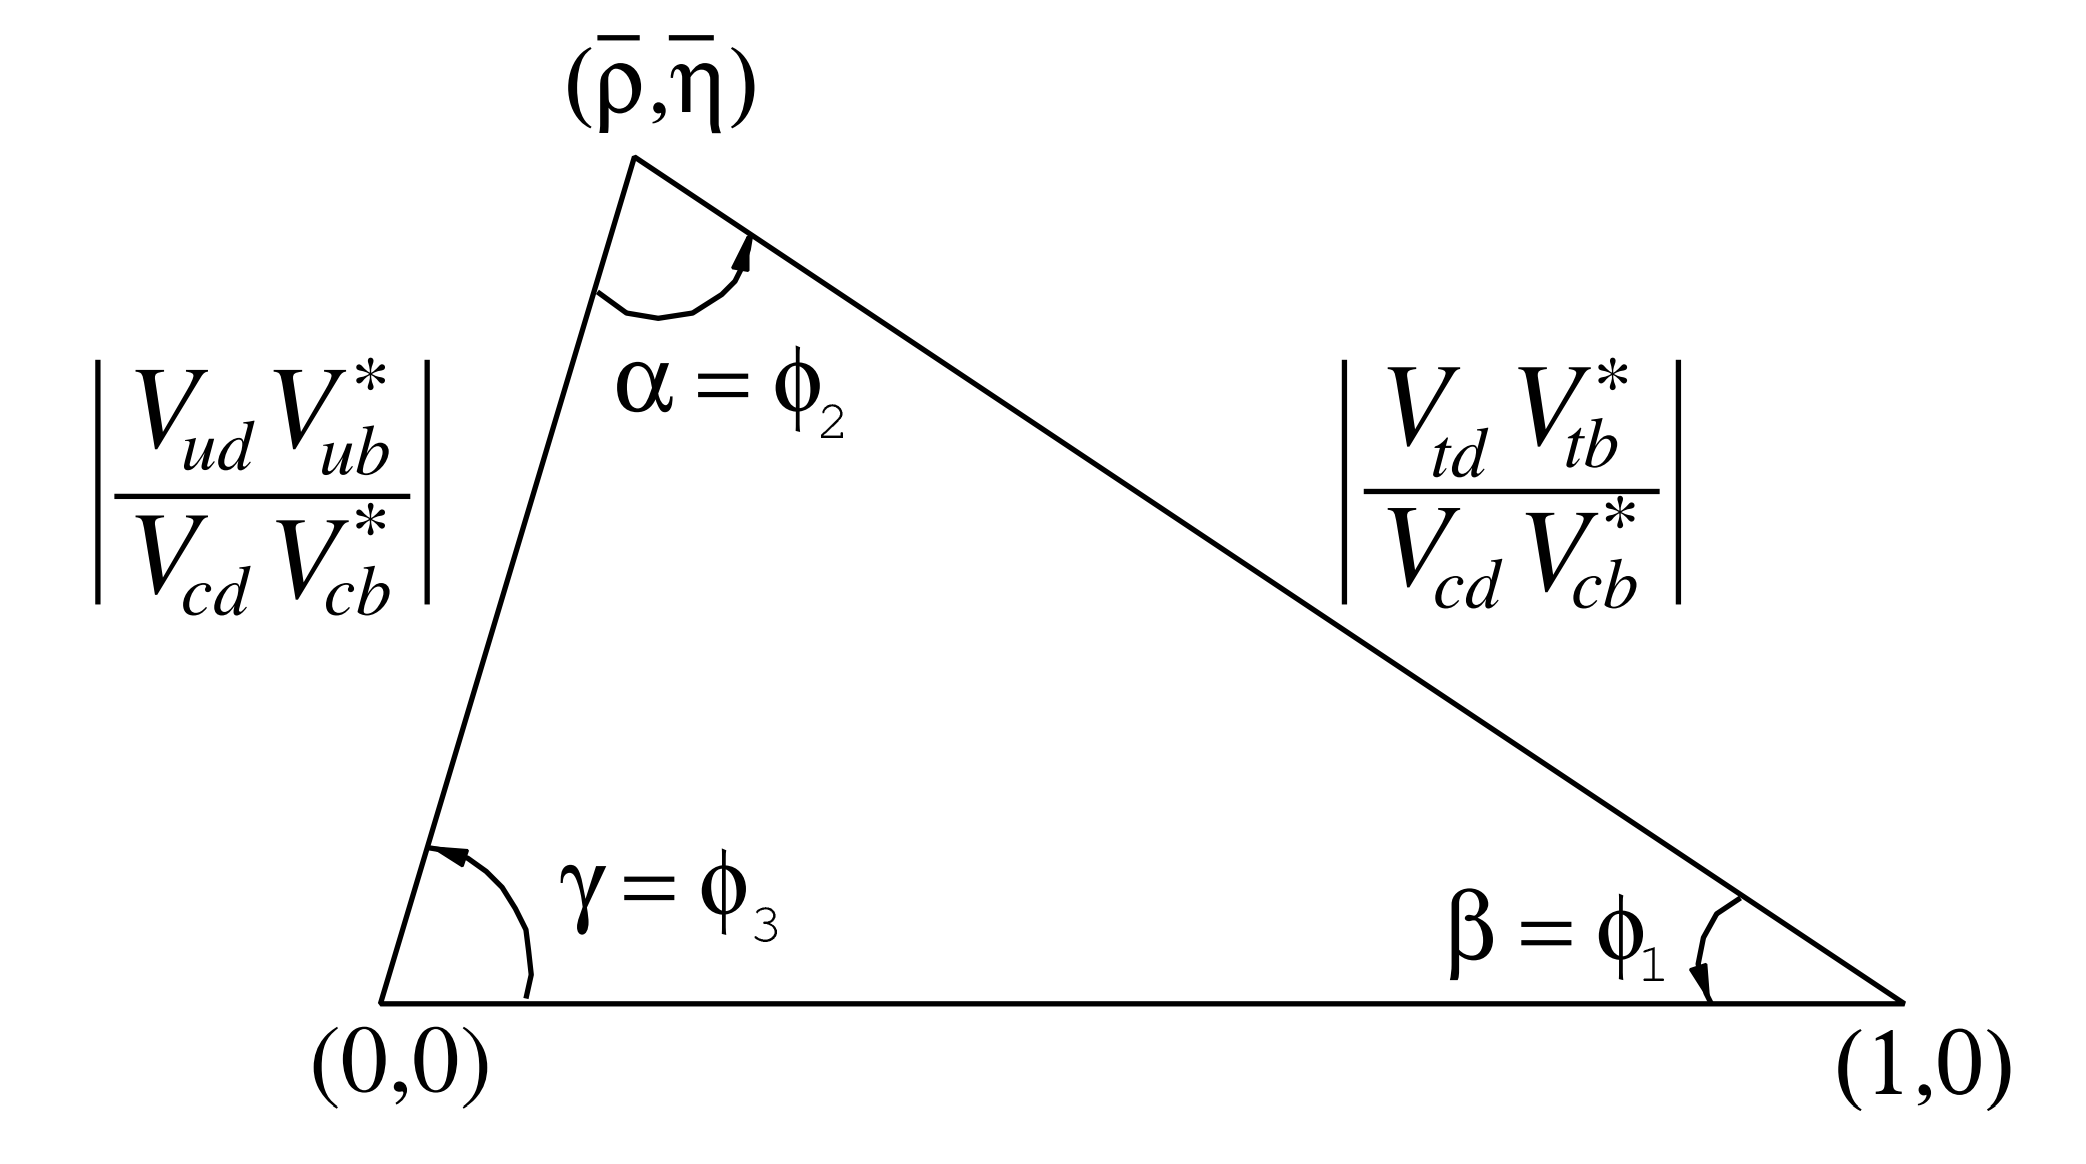
\includegraphics[width=0.7\columnwidth]{figures/theory/UT_definition.png}
    \caption{Definition of the lengths and sides of the Unitarity Triangle. Reproduced from the \emph{CKM Quark-Mixing Matrix} review of the PDG~\cite{PDG2020}.}
    \label{fig:UT_definition}
\end{figure}

\begin{figure}[tb]
    \centering
    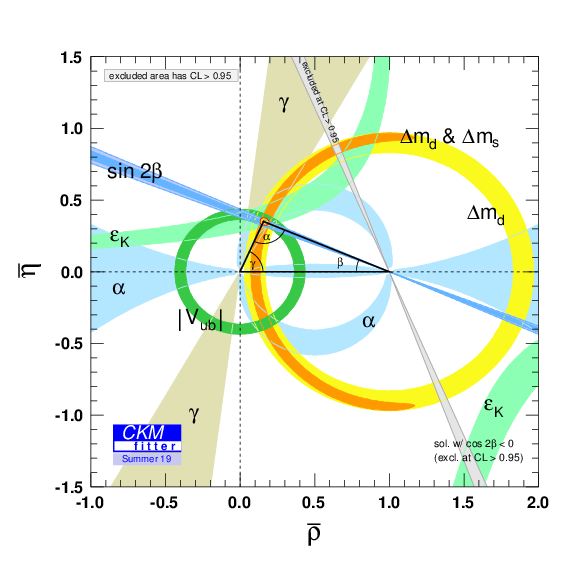
\includegraphics[width=0.7\columnwidth]{figures/theory/rhoeta_large.png}
    \caption{Current constraints on the Unitarity Triangle parameters as determined by the CKMFitter group for the EPS 2019 conference~\cite{CKMfitter2015}.}
    \label{fig:UT_constraints}
\end{figure}

Over-constraining the unitarity triangle by making separate measurements of all sides and angles, in as many different decay channels as possible, is an important and non-trivial test of the SM. The current experimental constraints are in agreement with the SM predictions, as visualised in Fig.~\ref{fig:UT_constraints}. 
The topic of the thesis is a measurement of the CKM angle
\begin{align}\label{eq:gamma_definition}
    \gamma \equiv \mathrm{arg} (-V_{ud}^{\phantom{*}}V_{ub}^*/V_{cd}^{\phantom{*}}V_{cb}^*)
    = \mathrm{arg} (-V_{cb}^{\phantom{*}}V_{cd}^*/V_{ub}^{\phantom{*}}V_{ud}^*).
\end{align}
From the Wolfenstein parameterisation in Eq.~\eqref{eq:CKM_Wolf}, it is can be seen that $\gamma$ equals the fundamental \CP-violating phase $\delta_\CP$ to $\mathcal O(\lambda^4)$. The angle $\gamma$ is unique among the CKM parameters, in that it can be easily measured in tree-level processes, without significant theoretical uncertainty from lattice QCD calculations~\cite{brodUltimateTheoreticalError2014}. Since $\gamma$ is (essentially) an input parameter in the SM, it is not possible to calculate a theoretical expectation that measurements can be compared to. However, tree-level processes are generally considered unlikely to be affected by Beyond-Standard-Model (BSM) effects. Therefore direct measurements of $\gamma$ can be considered a SM benchmark, to be compared with constraints based on measurements of other CKM elements that are measured in loop-level processes, and thus are more likely to be affected by BSM effects~\cite{blankeEmergingDeltaAnomaly2019}. These constraints are obtained in global fits, based on measurements of all CKM elements except $\gamma$, in which the unitarity of the CKM matrix is assumed to hold true. In practice, $\gamma$ is predominantly constrained by the value of $\beta$ and the elements defining the length of the side of the unitarity triangle opposite $\gamma$; the measurement of both rely on neutral \B mixing processes. If BSM physics effects enter the mixing loop, but is not accounted for in the global fit, it can result in the value of $\gamma$ that is determined in the global fit being different to the one obtained in direct measurements.
%This is illustrated with the two plots in Fig.~\ref{fig:ckm_matrix}. 
The current, worldwide combination of direct measurements published by the CKMFitter group is $\gamma = (72.1^{+5.4}_{-5.7})^\circ $, to be compared with the estimate from a global fit (without any $\gamma$ measurements) of $\gamma = (65.66^{+0.90}_{-2.65})^\circ $~\cite{CKMfitter2015}. 
Other world averages exist~\cite{HFLAV,UTfit-UT}, but the overall picture is the same: the ability to constrain BSM physics is currently limited by the uncertainty of the direct measurements. Hence further precision measurements of $\gamma$ are highly motivated. The precision is driven by time-integrated measurements of direct \CP-violation in $\Bpm\to\D\Kpm$ decays; such a measurement is the topic of this thesis and the theory behind is treated in detail in the following section. It is also possible to measure $\gamma$ in time-dependent mixing analyses of $\Bs\to\Dsmp\Kpm$, $\Bz\to\Dmp\pipm$, and related decays, by measuring \CP violation in interference between mixing and decay. These modes are expected to provide measurements with a precision of a few degrees in the future~\cite{lhcbcollaborationPhysicsCaseLHCb2019}.

% subsection the_ckm_matrix (end)




\subsection{\texorpdfstring{Measuring $\gamma$ in tree level decays}{Measuring gamma in tree level decays}} % (fold)
\label{sub:_measuring_gamma_in_tree_level_decays}

\begin{figure}[t]
    \centering
        \begin{subfigure}[t]{0.39\textwidth}
        \hspace{0.7cm}
        \begin{tikzpicture}[node distance=1cm and 1cm]
        \coordinate[label=left:$b$] (e1);
        \coordinate[right=of e1] (aux1);
        \coordinate[right=of aux1] (aux2);
        \coordinate[above=of aux2] (aux3);
        \coordinate[right=of aux2,label=right:$c$] (e2);
        \coordinate[right=of aux3] (e3);
        \coordinate[below=of e1] (e4);
        \coordinate[below=of e2] (e5);
        
        %
        \draw[particle] (e1) -- (aux1);
        \draw[longparticle] (3,-0.7) node[right]{$\bar u$} -- (0,-0.7) node[left]{$\bar u$} ;
        \draw[particle] (aux1) node[below]{$V_{cb}$} -- (e2);
        \draw[boson] (aux1) -- (2,1.05);
        \draw[particle] (3,0.7) node[right]{$\bar u$} -- (2,1.05) node[above]{$V_{us}^*$};
        \draw[particle] (2,1.05) -- (3,1.4) node[right]{$s$};

        
\end{tikzpicture}
        \caption{}
        \end{subfigure}
        \begin{subfigure}[t]{0.39\textwidth}
        \hspace{0.7cm}
        \begin{tikzpicture}[node distance=1cm and 1cm]
        \coordinate[] (e1);
        \coordinate[right=of e1] (aux1);
        \coordinate[right=of aux1] (aux2);
        \coordinate[below=of aux2] (aux3);
        \coordinate[right=of aux2] (e2);
        \coordinate[right=of aux3] (e3);
        \coordinate[below=of e1] (e4);
        \coordinate[below=of e2] (e5);
        
        %
        \draw[particle] (e1) node[left]{$b$} -- (aux1);
        \draw[longparticle] (3,-2.1) node[right]{$\bar u$} -- (0,-2.1) node[left]{$\bar u$};
        \draw[particle] (aux1) node[above]{$V_{ub}$}-- (e2) node[right]{$u$};
        \draw[boson] (aux1) -- (2,-1.05);
        \draw[particle] (2,-1.05) node[below]{$V_{cs}^*$} -- (3,-1.4) node[right]{$s$};
        \draw[particle] (3,-0.7) node[right]{$\bar c$} -- (2,-1.05);

        
\end{tikzpicture}
        \caption{}
        \end{subfigure}
        \caption{Tree level Feynman diagrams describing (a) ${\Bm\rightarrow \Dz \Km}$ and (b) ${\Bm\rightarrow \Dzb \Km}$ decays. The electro-weak phase difference between the two decays is $\Delta\phi = 
\text{arg}\left( {V_{cb}V_{us}^*}/{V_{ub}V_{cs}^*} \right)\simeq\gamma$.}
        \label{fig:feynman_diagrams}
    
\end{figure}

The phase $\gamma$ can be measured in tree-level processes with interference between $b\to c s \bar u$ and $b\to \bar c s u$ transitions. The canonical example, also the subject of this thesis, is based on measurements sensitive to interference between the $\Bpm\to\Dz\Kpm$ and $\Bpm\to\Dzb\Kpm$ decay amplitudes. As illustrated in Fig.~\ref{fig:feynman_diagrams} for the case of \Bm decays, the electro-weak phase difference between the two decays is $\Delta\phi = 
\text{arg}\left( {V_{cb}^{\phantom{*}}V_{us}^*}/{V_{ub}^{\phantom{*}}V_{cs}^*} \right)$. While $\Delta\phi$ is not identical to the definition of $\gamma$ in Eq.~\eqref{eq:gamma_definition}, the ratio of the involved CKM matrix elements is~\cite{grossmanEffectsBarMixing2014}
\begin{align}
-\frac{V_{cd}^*/V_{ud}^*}{V_{us}^*/V_{cs}^*} 
&= - \frac{
-\lambda [1-\frac{\lambda^4}{2}A^2(1-2(\rho-i\eta))](1-\frac{\lambda^2}{2}-\frac{\lambda^4}{8}(1+4A^2))
}
{\lambda(1-\frac{\lambda^2}{2}-\frac{\lambda^4}{4})} \notag \\
&= 1 - \lambda^4 A^2  (1 - 2(\rho -i\eta)) + \mathcal O(\lambda^5). 
\end{align}
The ratio equals unity to $\mathcal O(\lambda^4)\simeq 2.6\times 10^{-3}$, and thus $\Delta\phi\simeq\gamma$ is a good approximation within current experimental uncertainties. For the remainder of this thesis the approximation will be used without further comment. The diagrams in Fig.~\ref{fig:feynman_diagrams} describe the leading order contributions to the two amplitudes
\begin{subequations}\label{eq:B_amplitudes}
\begin{align}
\begin{split}    
    A[\Bm\to\Dz\Km] &\equiv A_B \\
    A[\Bm\to\Dzb\Km] &\equiv \bar A_B  \equiv r_B A_B e^{i(\delta_B - \gamma)},
\end{split}
\end{align}
where the last equality introduces two new parameters: the amplitude magnitude ratio $r_B\equiv |\bar A_B |/|A_B|$, and $\delta_B$, the strong-phase difference between the decay amplitudes.  Since all \CP-violation is attributed to the electro-weak phase in the SM, the \CP-conjugate decay amplitudes are~\cite{gronauDeterminingWeakPhase1991}
\begin{align}
\begin{split}    
    A[\Bp\to\Dzb\Kp] &= A_B \\
    A[\Bp\to\Dz\Kp]  &= \bar A_B = r_B A_B e^{i(\delta_B + \gamma)}.
\end{split}
\end{align}
\end{subequations}
In an experimental setting, the \Dz and \Dzb mesons are reconstructed in some final state, $f$, or its \CP-conjugate state, $\bar f$. In analogy with the \Bpm decays, the \D decay amplitude can be related\footnote{In this convention $\delta_D$ is thus phase of the suppressed \D-decay amplitude minus the phase of the favoured \D-decay amplitude. This is the opposite convention to that used in the \lhcb measurements with the ADS technique, but aligns with the phase definition used in the literature on $\gamma$ measurements in $\D\to\KS\pip\pim$ decays.} 
\begin{align}
\begin{split}\label{eq:D_amplitudes}
    A[\Dz\to f] &= A[\Dzb\to \bar f] = A_D \\ 
    A[\Dzb \to f] &= A[\Dz \to \bar f] = r_D A_D e^{i\delta_D}.
\end{split}
\end{align}
where the assumption has been made that \CP violation in the \D decays is negligible, and $\delta_D$ denotes a \CP-conserving strong-phase difference. While \CP-violation in \D decays has recently been measured~\cite{LHCb-PAPER-2019-006}, the size of the effect is small and it is considered negligible in this thesis. Based on Eqs.~\ref{eq:B_amplitudes}~and~\eqref{eq:D_amplitudes}, the decay rates of \Bp and \Bm mesons into the possible final states can be seen to satisfy 
\begin{subequations}\label{eq:rate_equations}
\begin{align}
    \Gamma(\Bm \to \D(\to f)\Km) & \propto 
    1 + r_D^2 r_B^2 + 2 r_B r_D \cos\left[\delta_B + \delta_D - \gamma\right], \label{eq:rate_Bm_f}\\
    \Gamma(\Bp \to \D(\to \bar f)\Kp) & \propto 
    1 + r_D^2 r_B^2 + 2 r_B r_D \cos\left[\delta_B + \delta_D + \gamma\right], \label{eq:rate_Bp_fbar}\\
    \Gamma(\Bm \to \D(\to \bar f)\Km) & \propto
    r_D^2 + \phantom{1}r_B^2 + 2 r_B r_D \cos\left[\delta_B - \delta_D - \gamma\right], \label{eq:rate_Bm_fbar}\\
    \Gamma(\Bp \to \D(\to f)\Kp) & \propto
    r_D^2 + \phantom{1}r_B^2 + 2 r_B r_D \cos\left[\delta_B - \delta_D + \gamma\right]. \label{eq:rate_Bp_f} 
\end{align}
\end{subequations}
The processes in Eqs.~\eqref{eq:rate_Bm_f}~and~\eqref{eq:rate_Bp_fbar} are \CP-conjugate and it is clear how, in the general case where $\delta_B+\delta_D\neq 0$,  a non-zero value of $\gamma$ leads to \CP violation in the form of differing decay rates. The same is true for the processes in Eqs.~\eqref{eq:rate_Bm_fbar}~and~\eqref{eq:rate_Bp_f}. Depending on the choice of \D final state, these expressions can be used to relate $\gamma$ to various observables that are experimentally accessible. This thesis concerns the choice $f=\KS\pip\pim$ or $f=\KS\Kp\Km$, where the terms related to the \D decay all have a non-trivial variation over the phase space of the decay. However, it is useful to first analyse the simpler case where $f$ is a two-body state. 

The simplest case is when $f$ is chosen to be a \CP eigenstate, so that $f=\pm\bar f$ and the rate equations~of~\eqref{eq:rate_Bm_f}--\eqref{eq:rate_Bp_f} simplify, because $r_D=1$ and $\delta_D\in\{0,\pi\}$. Measurements of $\gamma$ in such decay modes are denoted GLW measurements, after  Gronau, London, and Wyler who described the approach in the early 90ies~\cite{gronauDeterminingWeakPhase1991,gronauHowDetermineAll1991}. Experimentally it is preferable to measure yield ratios rather than absolute rates, and the observables of interest are thus the \CP asymmetry
\begin{subequations}\label{eq:GLW_observables}
\begin{align}
\begin{split}
    A_{\CP=\pm1} &= \frac{\Gamma[\Bm\to D_{\CP}\Km] - \Gamma[\Bp\to D_{\CP}\Kp]}{\Gamma[\Bm\to D_{\CP}\Km] + \Gamma[\Bp\to D_{\CP}\Kp]} \\
    &= \frac{\pm r_B \sin \delta_B \sin \gamma}{1 + r_B^2 \pm 2 r_B \cos \delta_B \cos \gamma},
\end{split}
\end{align}
as well as the ratio
\begin{align}
\begin{split}
    R_{\CP=\pm 1} &= 2\frac{\Gamma[\Bm\to D_{\CP}\Km] + \Gamma[\Bp\to D_{\CP}\Kp]}{\Gamma[\Bm\to \Dz\Km] + \Gamma[\Bp\to \Dzb\Kp]} \\
    &=  1 + r_B^2 \pm 2 r_B \cos \delta_B \cos \gamma.
\end{split}
\end{align}
\end{subequations}
In practice, $A_{\CP}$ and $R_{\CP}$ are obtained from measured yield ratios that are corrected with appropriate branching fractions. A measurement of $A_{\CP}$ and $R_{\CP}$ alone is not sufficient to determine the underlying physics parameters $(\gamma, r_B, \delta_B)$: even if $r_B$ was to be known exactly, the measurements only constrain the products $\cos \delta_B \cos \gamma$ and $\sin \delta_B \sin \gamma$ and will always allow four solutions for $(\gamma, \delta_B)$. 
%When combined with additional measurements that constrain $r_B$, measurements of $A_{\CP}$ and $R_{\CP}$ put quite stringent constraints on $\delta_B$ and $\gamma$, albeit with multiple, ambiguous solutions. For a given $\delta_B$ two different solutions exist for $\gamma$, and furthermore the equations are invariant under the exchange $\delta_B \leftrightarrow \gamma$, as well as the simultaneous transformation $(\gamma, \delta_B) \to (\gamma + \pi, \delta_B + \pi)$. Typical constraints on $(\gamma, r_B, \delta_B)$ for a measured set of GLW observables are illustrated in Fig.~\ref{fig:typical_GLW_constraints}, for observables corresponding to $(\gamma, r_B, \delta_B) = (75^\circ, 0.1, 130^\circ)$, which is fairly representative of the current, experimental average.\footnote{A full interpretation of $A_{\CP}$ and $R_{\CP}$ in terms of the underlying physics parameters also needs to take secondary effects, such as \D-mixing, into account. Such effects are ignored in this exposition, where the point is simply to illustrate the fundamental principles of the measurement strategy.} 
One way to break the ambiguity, first noted in the original paper~\cite{gronauDeterminingWeakPhase1991}, is to make further measurements in additional \B decays, such as the $\Bpm\to\Dstar\Kpm$ or $\Bz\to\D\Kstarz$ modes. These decays can also be described with the  formalism derived above, but will not share the same ambiguous solutions because the $r_B$ and  $\delta_B$ values are unique to a given \B decay. Another method is to analyse \D decay final states that are not \CP eigenstates.

A few years after the GLW method was proposed, Atwood, Dunietz, and Soni analysed an alternative choice of \D final states: a simultaneous analysis of a Cabibbo-favoured (CF) decay $\Dz\to f$ and the doubly-Cabibbo-suppressed (DCS) decay $\Dz\to \bar f$ into the \CP conjugate final state~\cite{atwoodEnhancedCPViolation1997,atwoodImprovedMethodsObserving2001}. Their suggested method is named the ADS method after the authors. The classical example is to take $f=\Km\pip$ and $\bar f = \pim\Kp$. The relative suppression means that the $r_D$ of Eq.~\eqref{eq:rate_equations} is small, typically of the same order of magnitude as $r_B$, and thus the \CP asymmetry of the suppressed decay is $\mathcal O(1)$:
\begin{subequations}\label{eq:ADS_observables}
\begin{align}
\begin{split}\label{eq:ADS_asym}
    A_{ADS(\bar f)} &= \frac{\Gamma[\Bm\to D(\to\bar f)\Km] - \Gamma[\Bp\to D(\to f)\Kp]}{\Gamma[\Bm\to D(\to\bar f)\Km] + \Gamma[\Bp\to D(\to f)\Kp]} \\
    &= \frac{r_Dr_B \sin (\delta_B - \delta_D) \sin \gamma}{r_D^2 + r_B^2 + 2 r_Dr_B \cos (\delta_B - \delta_D) \cos \gamma}.
\end{split}
\end{align}
The large \CP asymmetry is a prime feature of the ADS method. However, the suppressed-to-favoured yield ratio is also sensitive to the physics parameters of interest:
\begin{align}
\begin{split}
    R_{ADS(\bar f)} &= \frac{\Gamma[\Bm\to D(\to\bar f)\Km] + \Gamma[\Bp\to D(\to f)\Kp]}{\Gamma[\Bm\to D(\to f)\Km] + \Gamma[\Bp\to D(\to \bar f)\Kp]} \\
    &= \frac{r_B^2 + r_D^2 + 2 r_Dr_B \cos (\delta_B - \delta_D) \cos \gamma}{1 + r_D^2 r_B^2 + 2 r_Dr_B \cos (\delta_B + \delta_D) \cos \gamma}.
\end{split}
\end{align}
\end{subequations}
The interpretation of $A_{ADS}$ and $R_{ADS}$ in terms of $(\gamma, r_B, \delta_B)$ requires knowledge of the $r_D$ and $\delta_D$ parameters, but these can be measured independently~\cite{HFLAV}. In general, the constraints from a single set of ADS observables suffer from ambiguities similar to those in the GLW case. However, unlike the GLW case, each \D decay mode provides an independent set of constraints, because the parameters related to the \D decay vary. 

The discussion of this section has centred on the classical case of $\Bpm\to D\Kpm$ decays with a two-body \D final state. With minor modifications the techniques have been used to make measurements sensitive to $\gamma$ in \Bz decays, with \B decay final states including excited \D mesons or kaons, and in \BtoDpi decays (summaries of the measurements made by the \B factories and \lhcb can be found in Refs.~\cite{BelleCombo,BabarCombo,LHCb-PAPER-2016-032,LHCb-CONF-2018-002}). The $\Bpm\to D \pipm$ decay is also \CP-violating, although the effect is much smaller than in the $\Bpm\to D\Kpm$ decay because $r_B^{\D\pi}\simeq 0.005$~\cite{rDpi}, whereas $r_B^{\D K}\simeq 0.1$. Furthermore, it is possible to use multi-body \D final states. However, in some cases, a better precision can then be obtained by exploiting phase-space dependent decay rates. This is the topic of the next section.


% subsection _measuring_gamma_in_tree_level_decays (end)

\section{\texorpdfstring{Measuring $\gamma$ using multi-body D final states}{Measuring gamma using multi-body D final states}} % (fold)
\label{sec:gamma_with_multibody_d_final_states}


In multi-body \D decays, the $r_D$ and $\delta_D$ parameters of the fundamental decay rates in Eq.~\eqref{eq:rate_equations} vary over the phase space of the \D decay. This section describes a model-independent approach to measure $\gamma$ in $\B\to\D(\to\KS\pip\pim)h^\pm$ decays by exploiting this variation, where $h^\pm$ denotes a kaon or a pion. The theory is identical for $\D\to\Ks\Kp\Km$ decays, and similar ideas have been proposed for the $\D\to\Kp\pim\pim\pip$~\cite{evansImprovedSensitivityCKM2020}, $\D\to\KS\pip\pim\piz$~\cite{CLEOKSpipipi0}, and $\D\to2\pip2\pim$ modes~\cite{harnewModelindependentDeterminationStrong2018}. First, however, the formalism for describing amplitudes of multi-body decays is briefly reviewed.


\subsection{Dalitz plots and the phase space of multi-body decays} % (fold)
\label{sub:the_phase_space_of_multibody_decays_and_dalitz_plots}

In general, the phase space of the $n$-body decay $P\to p_1 + p_2 + ... + p_n$ consists of $n$ four momenta, with a total of $4n$ components. The requirement that each of the final state particles is on-shell provides $n$ constraints on these components, and energy-momentum conservation removes a further 4 degrees of freedom. If the original particle $P$ is s \emph{scalar}, the decay is isotropic, which removes an additional 3 degrees of freedom, leaving the total number of degrees of freedom at $3n-7$. For the specific case of three-body decays, the available phase space can thus be parameterised with only two parameters. A practical and often used choice is the invariant masses
\begin{align}\label{eq:dalitz_coords}
    s_{12} &= m^2(p_1p_2) = (p_1^\mu+p_2^\mu)^2, & s_{13} &= m^2(p_1p_3) = (p_1^\mu+p_3^\mu)^2.
\end{align}
The choice of particle pairs is arbitrary, and the coordinates easily related
\begin{align}
    m^2_P + m^2_{p_1} + m^2_{p_2} + m^2_{p_3} = m^2(p_1p_2) + m^2(p_1p_3) + m^2(p_2p_3).
\end{align}
A scatter plot of $(s_{12}, s_{13})$ values for a sample of particle decays is denoted a Dalitz plot~\cite{dalitzCXIIAnalysisTmeson1953}. It has the very useful feature that the presence of (narrow) resonances in the decay leads to visible bands in the scatter plot. Figure~\ref{fig:Dalitz_plot} illustrates how the limits of the Dalitz plot are defined by kinematic constraints, and shows an example of a Dalitz plot for $\Dz\to\KS\pip\pim$ decays in which the $K^*(892)^\pm$ and $\rho(770)$ resonances are clearly visible. 
%The plot shows the sample of $\Bp\to\D\pip$ decays used to make the measurement described in Chapter~\ref{ch:5-GGSZ-measurement} and thus the \D meson is in a superposition of \Dz and \Dzb states (as detailed in the following section). 

\begin{figure}[tb]
    \centering
    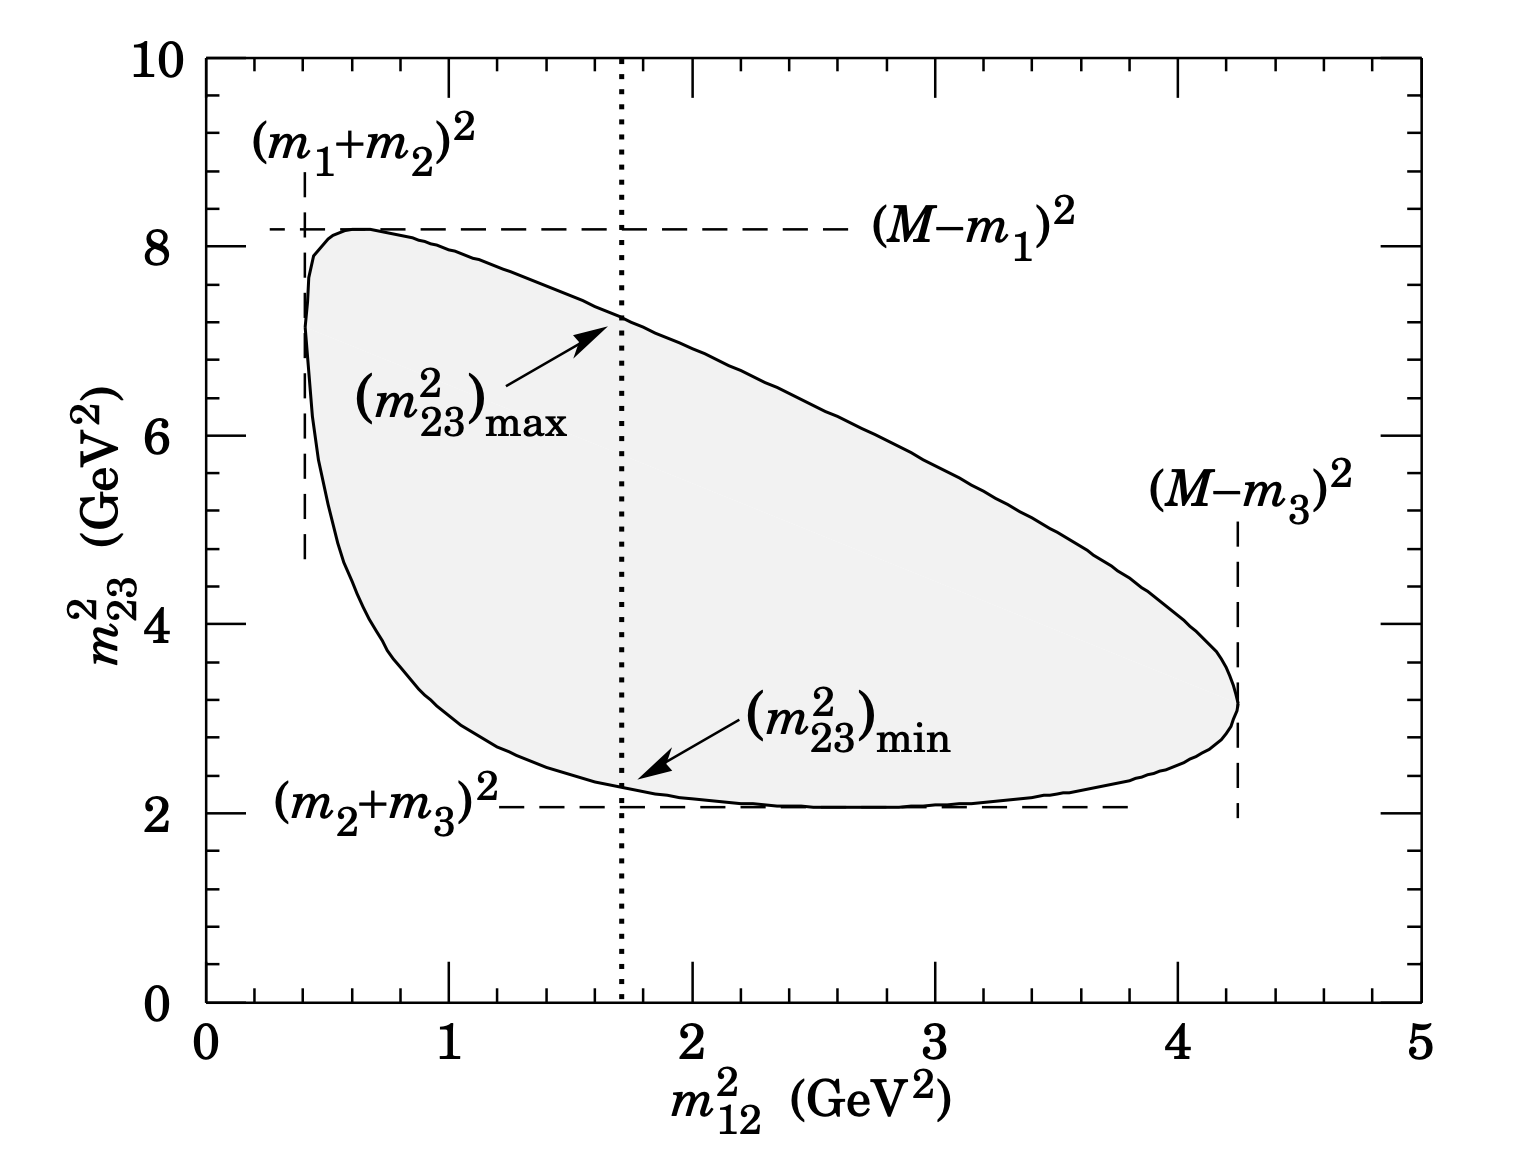
\includegraphics[height=5.5cm,valign=t]{figures/theory/Dalitz_definitions.png}
    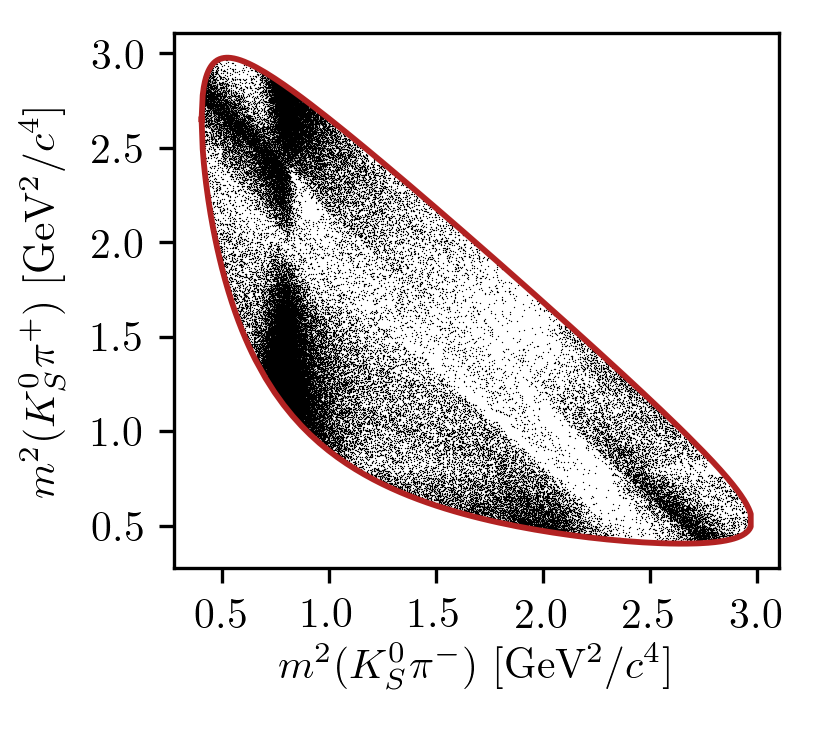
\includegraphics[height=6cm,valign=t]{figures/theory/single_DP_Pi_PiPi_LLandDD_minus.png}
    \caption{(Left) Schematic of a Dalitz plot and the limits of the kinematically allowed phase space. The dotted line illustrates how the possible values of $m^2_{23}=s_{23}$ are restricted to an interval for a given value of $m^2_{12}=s_{12}$. Reproduced from the \emph{Kinematics} review of the PDG~\cite{PDG2020}. (Right) Example of a Dalitz plot for $\Dz\to\KS\pip\pim$ decays in an \lhcb sample of flavour-tagged \Dz decays.}
    \label{fig:Dalitz_plot}
\end{figure}

In terms of the coordinates of Eq.~\eqref{eq:dalitz_coords} the differential decay rate is given by
\begin{align}
    \text d \Gamma = \frac{1}{32(2\pi)^3 m^3_P} |\mathcal M|^2 \,\text d s_{12} \text d s_{13},
\end{align}
where $\mathcal M$ is the QFT matrix element, or total decay amplitude, corresponding to the decay. In general, it is not possible to calculate $\mathcal M$ from first principles. Instead, the experimental analysis of multi-body decays typically rely on an amplitudes model defined with an empirically well motivated form, in which a number of free parameters must be determined experimentally. The simplest case is that of an \emph{isobar} model, where it is assumed that the full decay can be decomposed into consecutive two-body decays of the form $P \to R_{ij} (\to p_i + p_j) p_k$. Thus, $\mathcal M$ is expressed as a non-resonant constant amplitude term, $k_{NR}$, plus a sum of resonance terms
\begin{align}\label{eq:amplitude}
    \mathcal M (s_{12}, s_{13}) = k_{NR} + \sum_r k_r \mathcal M^r(s_{12}, s_{13}).
\end{align}
The exact form of the $\mathcal M^r$ function depends on the resonance in question. An overview is given in the PDG review on resonances and references therein~\cite{PDG2020}. The isobar formalism breaks down when resonances in the decay are not well separated. In this case, models of the form in Eq.~\eqref{eq:amplitude} can still be employed, if the contribution from overlapping resonances are collected in a single term. An example of such a model, is the amplitude model for $\Dz\to\KS\pip\pim$ decays developed by the Belle collaboration for a measurement of the CKM angle $\beta$ in 2018~\cite{Belle2018}. In this model, individual terms are included for $\Dz\to\Kstar(\to\KS\pi^\pm)\pimp$ decays, whereas the $\pi\pi$ and $K\pi$  $S$-wave contributions are modelled with the so-called $K$-matrix- and LASS formalisms~\cite{chungPartialWaveAnalysis1995,astonStudyPiScattering1988}. The amplitude and phase of $\mathcal M$ as predicted by this model are shown in Fig.~\ref{fig:amplitude_models}.

\begin{figure}[tb]
    \centering
    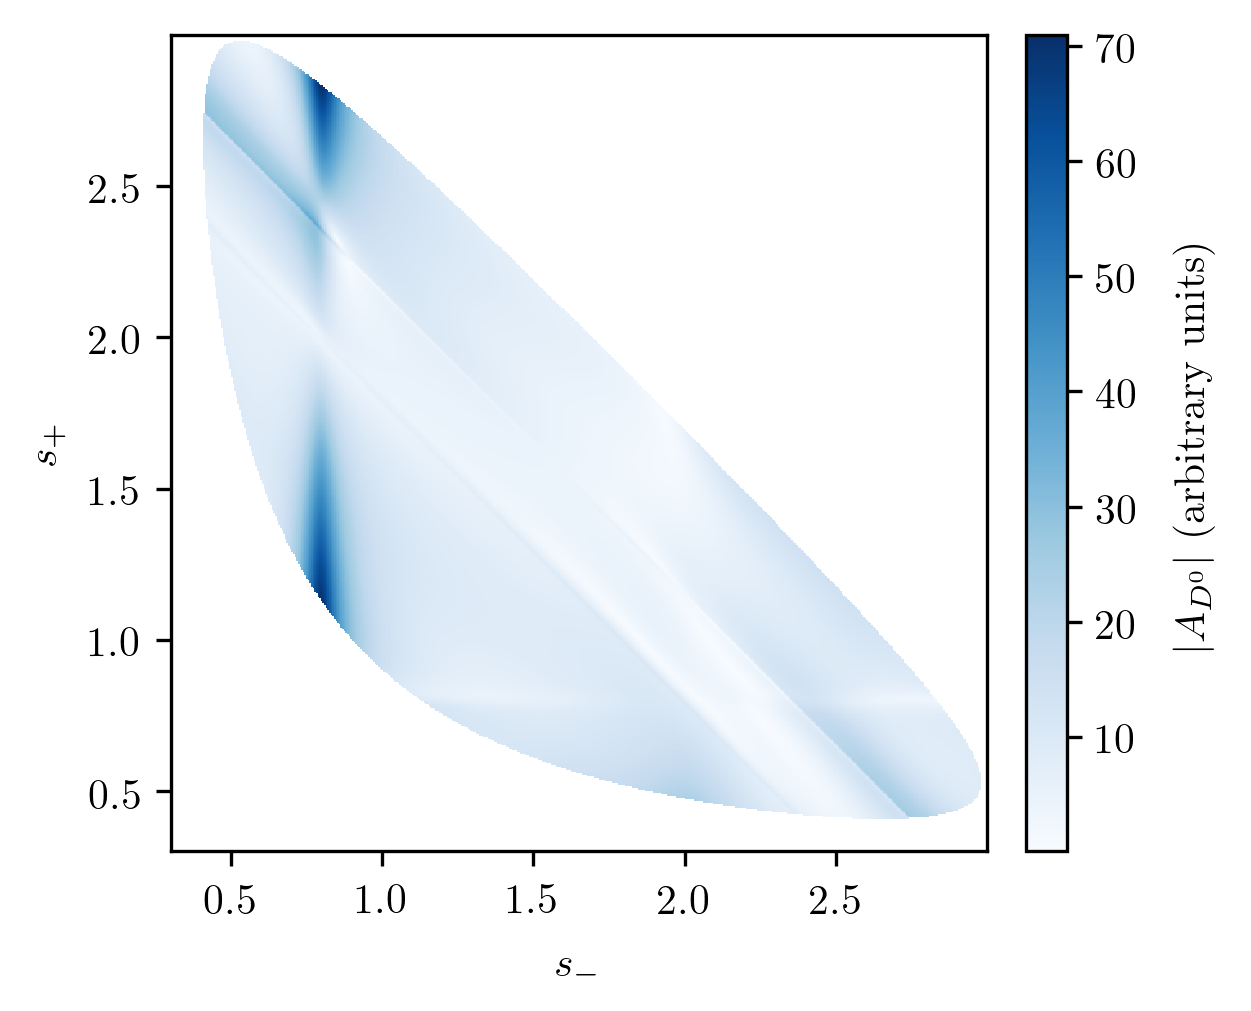
\includegraphics[width=0.48\columnwidth]{figures/theory/ampD.png}
    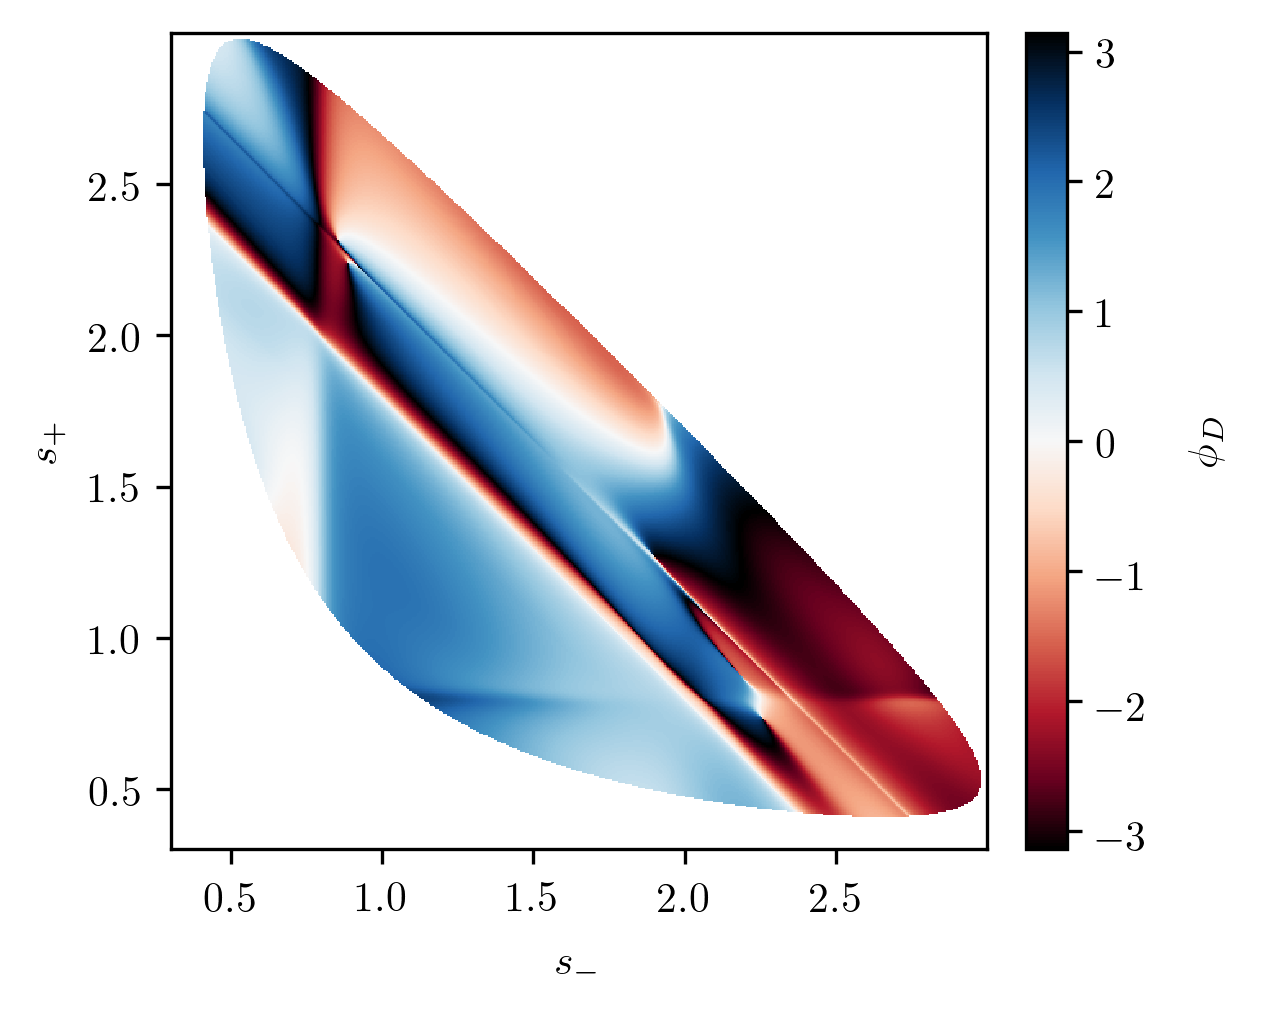
\includegraphics[width=0.48\columnwidth]{figures/theory/phiD.png}
    \caption{The (left) magnitude and (right) phase of the \DtoKspipi amplitude in the Belle 2018 model~\cite{Belle2018}.}
    \label{fig:amplitude_models}
\end{figure}
% subsection the_phase_space_of_multibody_decays_and_dalitz_plots (end)


\subsection{\texorpdfstring{The BPGGSZ method to measure $\gamma$}{The BPGGSZ method to measure gamma}} % (fold)
\label{sub:the_ggsz_method_to_measure_gamma}

% subsection the_ggsz_method_to_measure_gamma (end)
The non-trivial phase-space dependence of the $\D\to\KS\pip\pim$ decay amplitude can be exploited to measure $\gamma$ with $\Bpm\to \D\Kpm$ or $\Bpm\to \D\pipm$ decays. This approach was proposed independently by Bondar~and~Poluektov~\cite{BONDARGGSZ,BELLE2004} within the Belle collaboration, and by Giri, Grossman, Soffer, and Zupan~\cite{giriDeterminingGammaUsing2003}. It takes the commonly used acronym BPGGSZ after all these authors.\footnote{The "B" and "P" are a recent addition to the BPGGSZ acronym, in recognition of the role played by Bondar and Poluektov in the development of the method. For a history of the origins of the approach, see Ref.~\cite{ceccucciOriginsMethodDetermine2020}.} For this specific decay \sm and \sp are used to described the Dalitz coordinates $m^2(\KS\pim)$ and $m^2(\KS\pip)$, respectively, and the \D decay amplitude is a function of these coordinates
\begin{align}\label{eq:ADDb_definition}
\ADorDbS (\smpLong)= A(\DorDbar^0\to K^0_\text{S} \pi^+\pi^-).
\end{align}
To a good approximation the \KS meson is a \CP eigenstate, meaning that the $\KS\pip\pim$ state is self-conjugate. Assuming this approximation to be exact, and that \CP violation in the \D decay is negligible, the \D decay amplitudes satisfy the symmetry relation
\begin{align}\label{eq:KS_symmetry}
     \ADbS(\sm, \sp)=\ADS(\sp, \sm).
 \end{align} 
 The impact of the \KS meson \emph{not} being an exact \CP eigenstate is treated in detail in Chapter~\ref{ch:4-KS-CPV}. In order to simplify equations, the short-hand notation 
 \begin{align}
     (s_{-+})&=(s_-,s_+), &(s_{+-})&=(s_+,s_-)
 \end{align} will be employed for the remainder of the thesis, so that the relation in Eq.~\eqref{eq:KS_symmetry} can be expressed as $\ADbS(\smp)=\ADS(\spm)$. Thus, the rate equations of Eq.~\eqref{eq:rate_equations} for the $\D\to\KS\pip\pim$ decay mode are
 \begin{subequations}\label{eq:Gamma_Bminus}
\begin{align} 
    \rm {d} \Gamma^-(\smp) &\propto |\cASm|^2 = |\AB|^2|\AKS|^2 \notag \\
    &\qquad\times\left[|\ADS(\smp)|^2 + \rB^2 |\ADS(\spm)|^2 + 2\rB |\ADS(\smp)||\ADS(\spm)|\right .
    \notag \\
    &\quad\qquad \left. \times \left(\cos[\delta_D(\smp)]\cos[\dB-\g]+\sin[\delta_D(\smp)]\sin[\dB-\g]\right)\right], \\
    \rm {d} \Gamma^+(\smp) &\propto |\cASp|^2 = |\AB|^2|\AKS|^2 \notag \\
    &\qquad\times\left[|\ADS(\spm)|^2 + \rB^2 |\ADS(\smp)|^2 + 2\rB |\ADS(\smp)||\ADS(\spm)|\right .
    \notag \\
    &\quad\qquad \left. \times \left(\cos[\delta_D(\smp)]\cos[\dB+\g]-\sin[\delta_D(\smp)]\sin[\dB+\g]\right)\right].
\end{align}
\end{subequations}
Here, $A_\KS$ is the decay amplitude for the $\KS\to\pip\pim$ decay, the strong phase of the \D decay enters via 
\begin{align}
    {\delta_\D(\smp) = \phi_D(\smp) - \phi_D(\spm) = - \delta_D(\spm)},
\end{align} where $\phi_D(\smp)$ denotes the complex phase of the $\ADS(\smp)$ amplitude, and a standard trigonometric relation have been employed to factorise the terms depending on the complex phases of the \B and \D decays. It can be seen that in the case where $\gamma=0$ the \Bp and \Bm decay rates are symmetric if the Dalitz coordinates are exchanged: $\Gamma^+(\sm, \sp)=\Gamma^-(\sp, \sm)$. The presence of \CP violation in the \B decay breaks the symmetry. Therefore it is possible to measure \g (and the nuisance parameters \rB and \dB) from the phase-space distribution of $\Bpm\to\D(\to\KS \pi^+ \pi^-)h^\pm$ decays, given knowledge of $\ADS(\smp)$.

A series of measurements of \g have been made that use amplitude models of the \D decay \cite{BABAR2005,BABAR2008,BABAR2010, BELLE2004,BELLE2006,BELLE2010,LHCb-PAPER-2014-017,LHCb-PAPER-2016-007}. However, 
a model-independent approach was proposed in the original GGSZ paper~\cite{giriDeterminingGammaUsing2003}, and developed further by Bondar and Poluektov~\cite{bondarFeasibilityStudyModelindependent2006,bondarUseQuantumcorrelatedD02008}. It relies on binning phase-space, in which case the necessary information on the \D decay amplitude can be summarised in a small set of coefficients that can be measured in a separate experiment. That is the approach followed in this thesis, and has been used previously by the Belle~\cite{BELLEMODIND} and \lhcb collaborations~\cite{LHCb-PAPER-2012-027,LHCb-PAPER-2014-041,LHCb-PAPER-2018-017}. It is described in detail in the following section.

Such a model-independent approach is favourable for two reasons. Firstly, estimating the systematic uncertainty related to the choice of parameterisation in an amplitude model is non-trivial. The BPGGSZ method relies heavily on knowledge of $\delta_D(\sm, \sp)$, yet the amplitude model parameters are determined in samples of flavour tagged \Dz and \Dzb decays, where only the magnitude of the amplitude is probed directly. Model-related uncertainties are determined by varying the model parameters within uncertainties, as well as repeating the analysis with alternative models where, for example, the included set of resonance contributions are changed, or alternative parameterisations are employed for some contributions. This is a somewhat subjective procedure, best exemplified by the fact that the \babar and \belle collaborations assigned very different uncertainties on their legacy BPGGSZ measurements of $\gamma$. The \babar collaboration assigned a model-related uncertainty on $\gamma$ of $3^\circ$~\cite{BABAR2010}, much smaller than the $8.9^\circ$ assigned in the \belle paper~\cite{BELLE2010}. The authors of the latter paper observe that the main uncertainty contribution is precisely due the imperfect knowledge of the phase of the amplitude, even in the case where a model perfectly describes the data. In the model-independent approach described below, this uncertainty is avoided in exchange for a statistically dominated measurement uncertainty that is trivial to determine. 
Secondly, in the precision era it is favourable that any experiment is easy to reinterpret in  extensions of the SM. This is non-trivial for an experiment that relies on determining a set parameters in a specific model, in which the parameters are only indirectly related to physically observable quantities. On the contrary, it is non-problematic for for an experiment that measures a small set of well-defined, model-independent physical observables. The model-independent approach described below does sacrifice some statistical performance due to the necessity of binning phase space: the statistical uncertainties on $\gamma$ are 10--20\,\% larger than in unbinned, model-dependent measurements~\cite{bondarUseQuantumcorrelatedD02008}. However, a slightly reduced statistical performance is preferable to a dominating, model-dependent systematic uncertainty when $\gamma$ is to serve as a high-precision SM benchmark; this motivates the approach followed in the thesis.

An alternative model-independent approach has recently been proposed by Poluektov~\cite{poluektovUnbinnedModelindependentMeasurements2018} where the externally measured input on the \D-decay phase are Fourier expansion coefficients, and which therefore avoids binning phase space. The approach may have the potential to improve the obtainable precision in the future, but this has yet to be demonstrated in an experimental setting.


\subsection{A model-independent approach} % (fold)
\label{sub:a_model_independent_approach}


The phase-space distribution can be analysed in a model-independent way, if the $\D$-decay phase space is split into regions, or bins, and the $\B$ decay yield in each bin determined experimentally. A measurement of $\gamma$ using this approach is the main topic of the thesis. This section describes the fundamental principle, whereas the details pertaining to the exact experimental approach are delegated to Section~\ref{sec:strategy_for_lhcb_measurement}. 

\begin{figure}[tb]
     \centering
     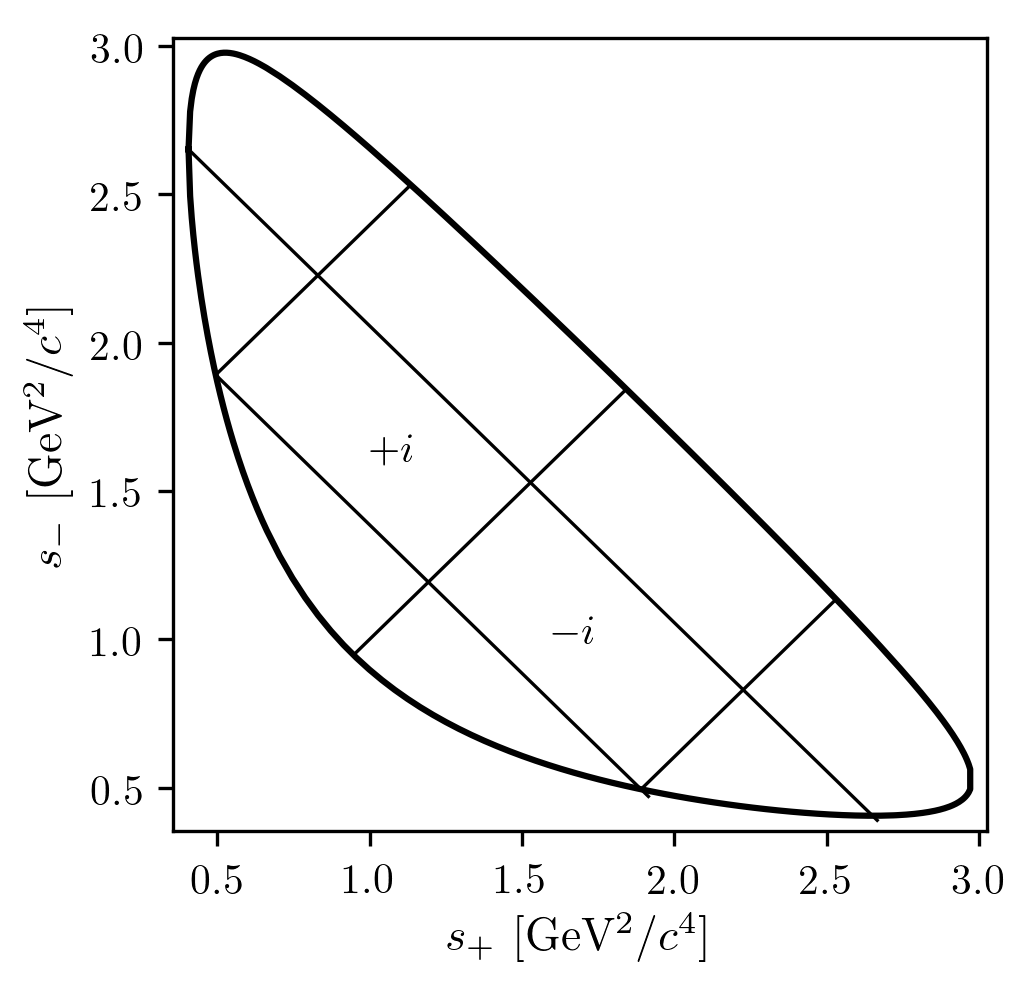
\includegraphics[width=0.55\columnwidth]{figures/theory/binnings/binning_example.png}
     \caption{Illustration of the binning principle used in BPGGSZ measurements: the bins are symmetric around the $m^2(\KS\pip)=m^2(\KS\pim)$ diagonal, and numbered so that opposite bins have the same number, except with opposite sign.}
     \label{fig:GGSZ_bin_principle}
 \end{figure} 

The amplitude symmetry of Eq.~\eqref{eq:KS_symmetry} is exploited by defining $2\mathcal N$ bins to be symmetric symmetric around the $\sm=\sp$ diagonal of the Dalitz plot, numbered $i=-\mathcal N$ to $\mathcal N$ (omitting zero) such that if the point $(\sm, \sp)$ is in bin $i$, then $(\sp, \sm)$ is in bin $-i$, and by convention $i>0$ for bins where $s_- >s_+$. The principle is illustrated in Fig.~\ref{fig:GGSZ_bin_principle}, but the binning schemes used in actual measurements are more complicated. The decay rates in Eq.~\eqref{eq:Gamma_Bminus} can be integrated over such bins, and give the bin yields
\begin{align}
\begin{split}    \label{eq:base_GGSZ_yields}
    N^-_i &\propto h^- \left[\Ki + \rB^2\Kmi + 2\sqrt{\Ki\Kmi}\left(\ci\xm+\si\ym\right)\right], \\
    N^+_i &\propto h^+ \left[\Kmi + \rB^2\Ki + 2\sqrt{\Ki\Kmi}\left(\ci\xp-\si\yp\right)\right],
\end{split}
\end{align}
where the parameters describing the \B decay have been expressed in terms of the observables
\begin{align}
    \xpm &= \rB \cos (\dB \pm \g), & \ypm &= \rB \sin (\dB \pm \g),
\end{align}
 and a number of phase-space integrated quantities related to the \D-decay have been introduced. The $K_i$ parameters denote the fractional yield of a flavour-tagged \Dz decaying into bin $i$, defined as
\begin{align}\label{eq:base_ki}
    K_i &= \frac{1}{N_K}\int_i\text{d}s^2 |\ADS(\smp)|^2, &
    N_K &=\int\text{d}s^2 |\ADS(\smp)|^2,
\end{align}
where $\int_i \text d s^2$ denotes integration over bin $i$ of the Dalitz plot. The \ci and \si denote the amplitude-weighted average of $\cos \delta_D(\smp)$ and $\sin \delta_D(\smp)$ over bin $i$
\begin{align}\label{eq:ci_si}
\begin{split}
    \ci &= \frac
    {\int_i \text{d}s^2 |\ADS(\smp)||\ADS(\spm)|\cos[\delta_D(\smp)]}
    {\sqrt{\int_i \text{d}s^2 |\ADS(\smp)|^2}\sqrt{\int_i \text{d}s^2 |\ADS(\spm)|^2}}, \\
    \si &= \frac
    {\int_i \text{d}s^2 |\ADS(\smp)||\ADS(\spm)|\sin[\delta_D(\smp)]}
    {\sqrt{\int_i \text{d}s^2 |\ADS(\smp)|^2}\sqrt{\int_i \text{d}s^2 |\ADS(\spm)|^2}}.
\end{split}
\end{align}
By the symmetry properties of $\delta_D(\smp)$ these parameters satisfy ${c_i=c_{-i}}$ and ${s_i=-s_{-i}}$. The normalisation constants $h^+$ and $h^-$ are identical in the ideal case, but it is convenient to define them separately for practical reasons: depending on the experimental setup, there may be overall production and detection asymmetries that affect the total signal yields. If an experimental analysis measures the \CP observables $(\xpm, \ypm)$ and the normalisations $h^\pm$ separately, based on the expressions in Eq.~\eqref{eq:base_GGSZ_yields}, the analysis is insensitive to these effects, because they are absorbed into the normalisation constants (as long as they are constant over the \D-decay phase space). This comes at the cost that the information on \xpm and \ypm from the overall yield asymmetry is lost, but Section~\ref{sub:relation_to_glw_and_ads_measurements} will show the loss in precision to be minimal.

Thus, for a set of 2$\mathcal N$ bins, the bin yields of Eqs.~\eqref{eq:base_GGSZ_yields} provide $4\mathcal N$ constraints on a total of $4\mathcal N+5$  parameters: $(h^\pm, K_i, c_i, s_i, x_\pm, y_\pm)$.\footnote{There are $2\mathcal N$ different $K_i$ parameters but only $2\mathcal N -1$ of them are independent, as they are constrained to sum to unity by definition.} However, the $K_i$, $c_i$, and $s_i$ parameters relate only to the \D decay, and can thus, in principle, be measured in independent experiments. With such external inputs, a measurement of the $\Bpm\to D(\to\KS\pip\pim)h^\pm$ yields in a set of bins can be used to constrain \xpm and \ypm, and thereby $(\gamma, r_B, \delta_B)$. The measurement presented in this thesis determines the $K_i$ parameters directly, but uses externally measured values of \ci and \si as input, as measured in quantum correlated \D decays by the CLEO~\cite{CLEOCISI} and BESIII~\cite{BESCISI,BESCISIKSKK} collaborations. Because these measurements are the foundation of the approach, they are described in some detail in the following section. In the future, it is possible that the \ci and \si parameters may be measured in charm-mixing measurements~\cite{thomasModelindependentOverlineDMixing2012}.




\subsection{Measuring strong-phase inputs at charm factories} % (fold)
\label{sub:measuring_strong_phase_inputs_at_charm_factories}

The strong-phase parameters $c_i$ and $s_i$ have been measured by the CLEO and BESIII collaborations using quantum correlated \Dz\Dzb pairs from decays of the $\psi(3770)$ resonance state, itself produced in $e^+e^-$ collisions at the resonance energy. The $\psi(3770)$ has quantum-number $C=-1$, which is conserved in the strong decay into two \D mesons, and thus the two \D mesons are produced in an anti-symmetric wave function. By observing the decay of one \D meson into a specific final state, say a \CP eigenstate, the quantum state of the other \D meson can be determined. The measurement is based on decays where both \D decays are reconstructed, one in the $\KS\pip\pim$ final state, the other in one of several different tag categories. The main principles are outlined below, but most experimental considerations and implementation details are left out for the sake of brevity.

The simplest case is when one \D meson decays into a final state that uniquely tags the flavour, such as $\Dzb\to\Kp e^-\bar\nu_e$. In that case, the \D meson decaying to $\KS\pip\pim$ is known to be in the \Dz state and the decay rate is simply determined by $\ADS: \Gamma(\smp)\propto |\ADS(\smp)|^2$. This allows for a measurement of the $K_i$ parameters.

If one \D meson is reconstructed in a \CP-even state, eg. $\Kp\Km$, or a \CP-odd state, eg. $\KS\piz$, the \D meson decaying to $\KS\pip\pim$ is known to be in a state of opposite \CP. Thus, for a tag-decay of $\CP=\pm1$ the decay rate has the form
\begin{subequations}
\label{eq:CP_cisi}
\begin{align}
    \Gamma_{\CP=\pm1} \propto \left| \ADS(\smp) \mp \ADS(\spm)\right|^2
\end{align}
and the bin yields will be given by
\begin{align}
    M_i^\pm \propto K_i + K_{-i} \mp 2 \sqrt{K_i K_{-i}}c_i.
\end{align}
\end{subequations}
Thus a simultaneous analysis of flavour and \CP tagged decays allow for a determination of the $K_i$ and \ci parameter sets.

Finally, the case where both \D mesons, for now denoted \D and $\D'$, decay into the $\KS\pi\pi$ final state can be considered. The total amplitudes have contributions from the case where \D is in the \Dz state and $\D'$ is in the \Dzb state, as well as the opposite flavour assignment. Thus the decay rate satisfies
\begin{subequations}\label{eq:Kspipi_cisi}
\begin{align}
    \Gamma_{\CP=\pm1} \propto \left| \ADS(\smp)\ADS(\spm') + \ADS(\spm)\ADS(\smp')\right|^2
\end{align}
where \smp denotes the Dalitz-plot coordinates of the \D meson, and $\smp'$ those of the $\D'$ meson. Defining $M_{ij}$ to be the yield of decays where the \D decay is in bin $i$ and the $\D'$ in bin $j$, the bin yields satisfy
\begin{align}
    M_{ij} \propto K_iK_{-j} + K_jK_{-i} - 2\sqrt{K_iK_{-i}K_jK_{-j}}\left(c_ic_j + s_is_j\right).
\end{align}
\end{subequations}
Thus, analysing these decays in addition to the \CP and flavour tagged decays provide information on all of $K_i$, \ci, and \si. Note, however, that Eqs.~\eqref{eq:CP_cisi} and \eqref{eq:Kspipi_cisi} are invariant under the transformation $\delta_D\to-\delta_D$. In practice, the analysis is extended in a number of ways to enhance the statistics: using "flavour-tag" states that are not exact flavour tags, such as $\Km\pip$, using self-conjugate multi-body \D-decay final states that are not exact \CP eigenstates, such as $\pip\pim\piz$, and using the \KL\pip\pim final state as well. However, the main principles are the same as described above.

The measurements of \ci and \si are made for a range of different binning schemes. It was noted already in Ref.~\cite{bondarUseQuantumcorrelatedD02008} that a rectangular binning scheme, such as the example in Fig.~\ref{fig:GGSZ_bin_principle}, does not provide the optimal sensitivity to $\gamma$. It will always be the case that some statistical sensitivity is lost in a binned analysed, as compared to an unbinned, model-dependent analysis; however, the degree to which this is the case depends on the choice of binning. A better sensitivity can be obtained if the bins are defined such that $\delta_\D$ is approximately constant over a given bin, by defining bin $i$ out of $\mathcal N$ via the condition
\begin{align} \label{eq:equal_binning_definition}
    \text{bin}_i = \left\{ (s_-, s_+)\quad  | \quad 2\pi (i-3/2)/\mathcal N \,<\, \delta_D(\sm, \sp) \,<\, 2\pi \times (i-1/2)/\mathcal N  \right\}.
\end{align}
In practice, the binning scheme is defined by splitting the \D-decay phase-space into quadratic \emph{micro bins} with a width of 0.0054 $(\gevcc)^2$ and assigning a bin number to each micro bin via the condition in \eqref{eq:equal_binning_definition} as evaluated in an amplitude model of choice. The obtained binning scheme when using an amplitude model developed by the \babar collaboration in 2008~\cite{BABAR2008} is shown in Fig.~\ref{fig:kspipi_bins_equal}. In Ref~\cite{bondarUseQuantumcorrelatedD02008} it was also shown that the binning can be even further optimised for sensitivity. The suggested figure of merit is
\begin{align}
    Q^2 = \frac
    {\sum_i \left(\frac{1}{\sqrt{N_i^{\B}} }\frac{\text d N_i^{\B}}{\text d x} \right)^2 + \left(\frac{1}{\sqrt{N_i^{\B}}} \frac{\text d N_i ^{\B}}{\text d y} \right)^2}
    {\int \text d s^2 \left[\left(\frac{1}{|\Gamma^{\B}(\smp)|}\frac{ \text d |\Gamma^{\B}(\smp)|^2 }{ \text d x}\right)^2 + \left(\frac{1}{|\Gamma^{\B}(\smp)|}\frac{ \text d |\Gamma^{\B}(\smp)|^2 }{ \text d y}\right)^2 \right]}
\end{align}
which quantifies the statistical sensitivity for a given binning, relative to the one achievable in an unbinned analysis. The CLEO collaboration defined an \emph{optimal} binning scheme by an iterative procedure where, starting from the equal binning scheme, a micro-bin is randomly reassigned new bin numbers in each step, and a step accepted if $Q^2$ increases. The optimisation is done for the case where $x=y=0$ and thus $Q^2$ simplifies to $Q^2_{x=y=0}=\sum_i N_i^{x=y=0}(c_i^2+s_i^2)/N_{total}^{x=y=0})$. The resulting binning scheme is shown in Fig.~\ref{fig:kspipi_bins_opt}. An additional binning scheme is defined, denoted the \emph{modified optimal} scheme and shown in Fig.~\ref{fig:kspipi_bins_modopt}, where the $Q^2$ figure of merit is modified to take into account the presence of backgrounds~\cite{CLEOCISI}. The modified optimal binning scheme has proven beneficial to use in measurements with small signal yields~\cite{LHCb-PAPER-2016-006}, but is not employed in the present thesis. 

Both the CLEO~\cite{CLEOCISI} and BESIII~\cite{BESCISI} collaborations have measured the values of \ci and \si for the equal, optimal, and modified optimal binning schemes. The results are also shown in Fig.~\ref{fig:kspipi_bins}, where they are  compared to the expectation from the latest amplitude model~\cite{Belle2018}. The measurements presented in this thesis are based on a combination of the BESIII and CLEO results for the optimal binning scheme, made by the BESIII collaboration~\cite{BESCISI} and tabulated in Table~\ref{tab:cisi}. 

\begin{figure}[p]
    \centering
    \begin{subfigure}{\columnwidth}
        \centering
        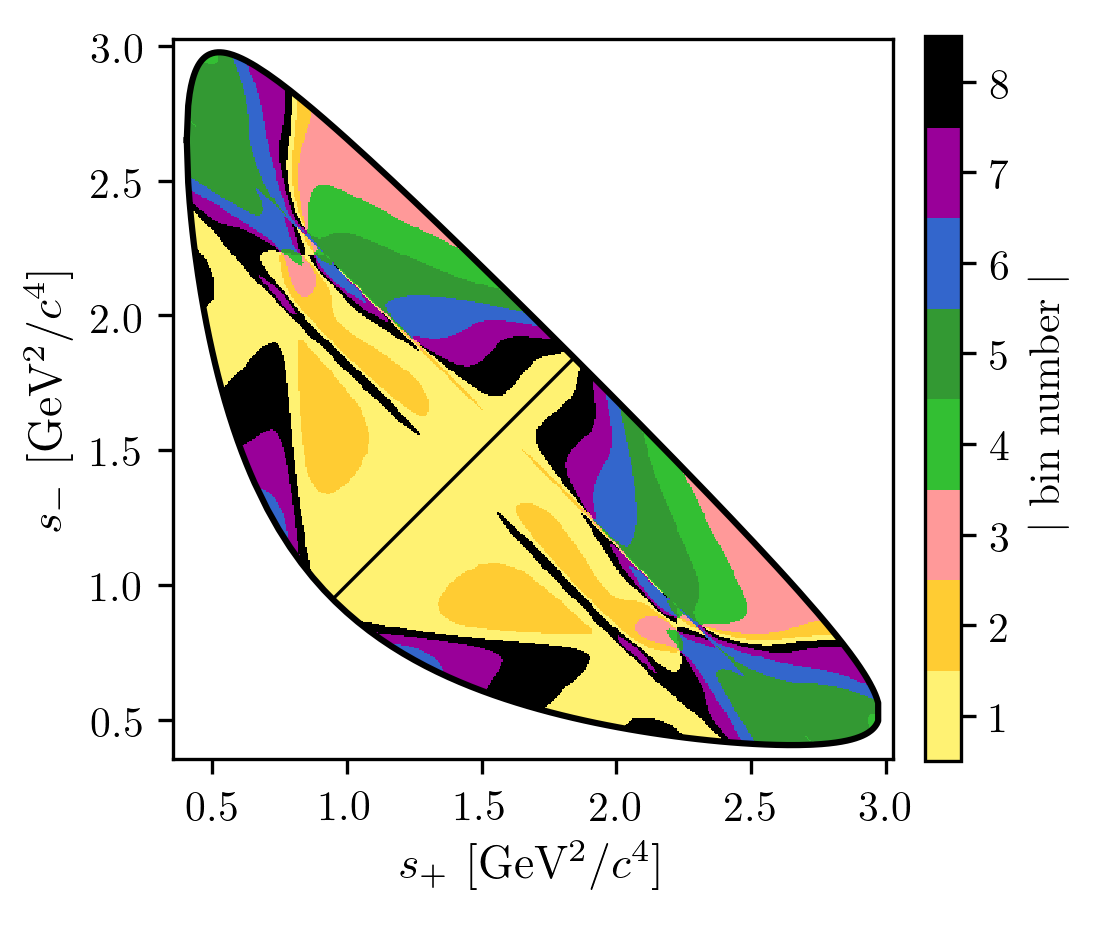
\includegraphics[height=5cm]{figures/theory/binnings/KsPiPi_equal.png}
        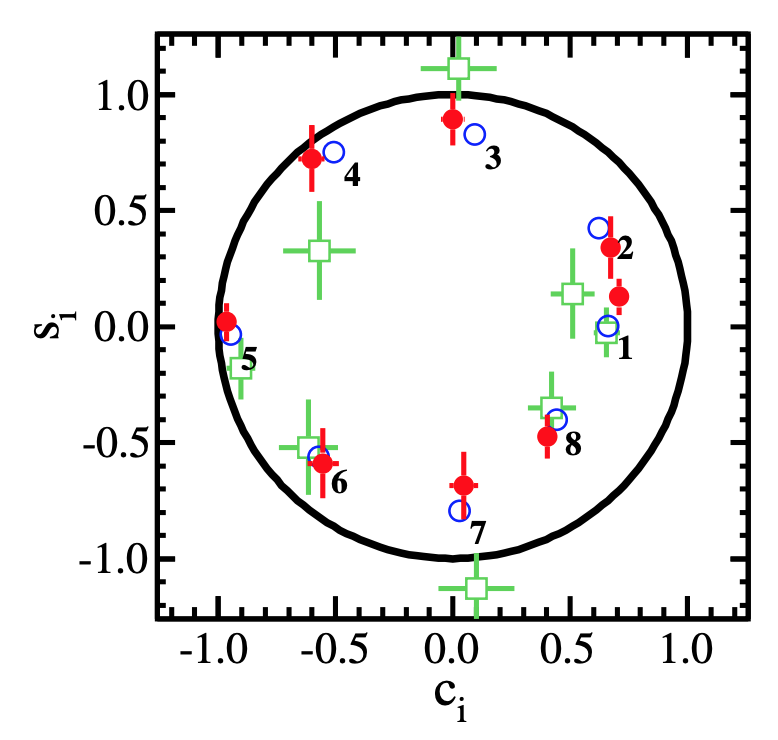
\includegraphics[height=5cm]{figures/theory/cisi_equal.png}
        \caption{}
        \label{fig:kspipi_bins_equal}
    \end{subfigure}
    \begin{subfigure}{\columnwidth}
        \centering
        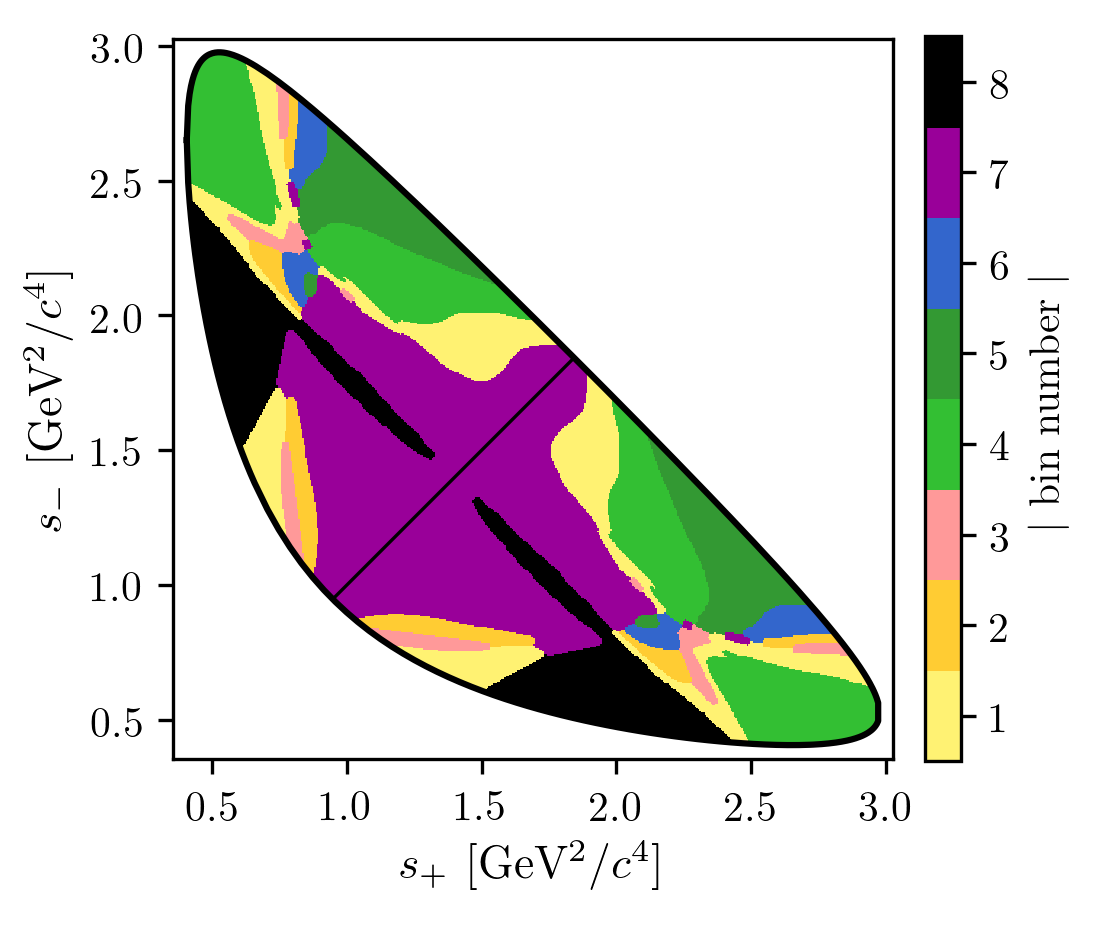
\includegraphics[height=5cm]{figures/theory/binnings/KsPiPi_optimal.png}
        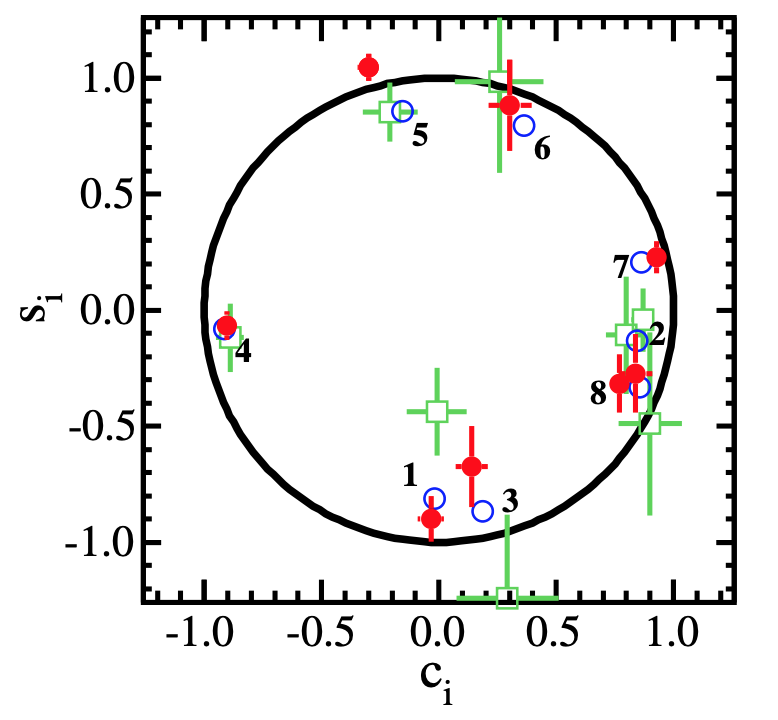
\includegraphics[height=5cm]{figures/theory/cisi_optimal.png}
        \caption{}
        \label{fig:kspipi_bins_opt}
    \end{subfigure}
    \begin{subfigure}{\columnwidth}
        \centering
        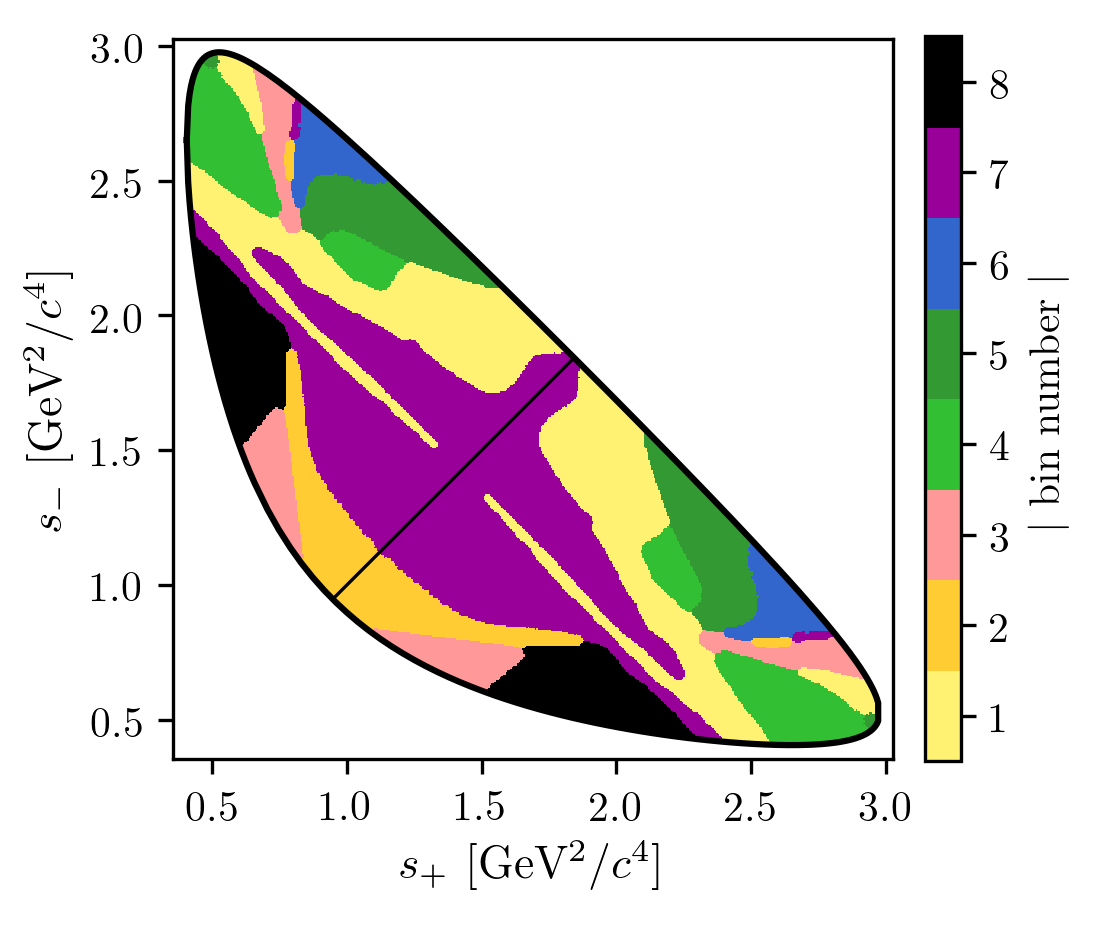
\includegraphics[height=5cm]{figures/theory/binnings/KsPiPi_mod_optimal.png}
        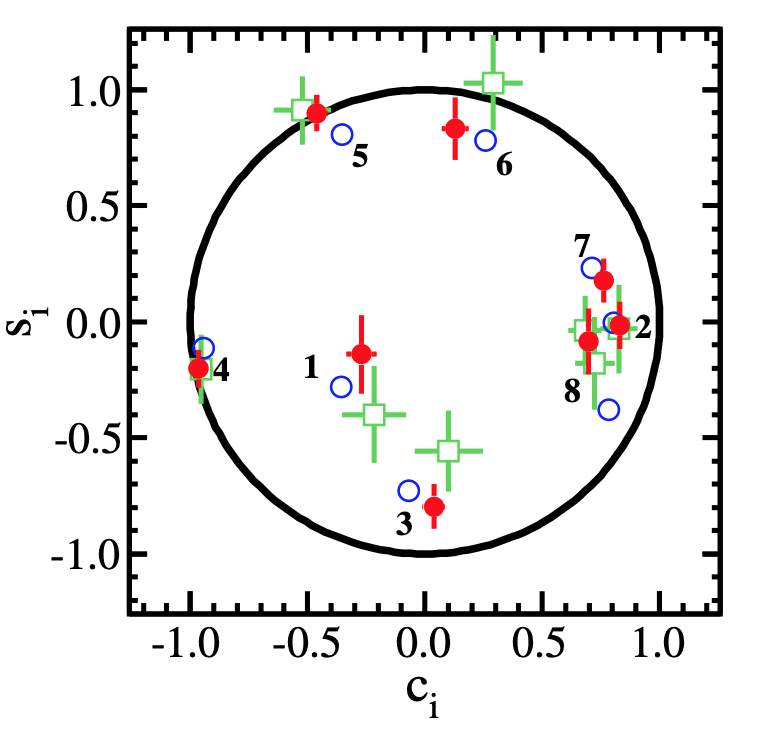
\includegraphics[height=5cm]{figures/theory/cisi_modified_optimal.png}
        \caption{}
        \label{fig:kspipi_bins_modopt}
    \end{subfigure}
    \caption{The (left) binning schemes and (right) measured values of $(\ci,\si)$ for the (a) equal, (b) optimal, and (c) modified optimal binning schemes for \DtoKspipi decays. The plots of the measured values are taken from Ref.~\cite{BESCISI} and show the results obtained by (red) BESIII, (green) CLEO, and (blue) the model expectation using the model from Ref.~\cite{Belle2018}.
    The measurement featured in this thesis uses the optimal binning scheme. Due to a different sign convention for the bin numbers, the \si values shown in the \besiii figures have the opposite sign to those defined in the text.}
    \label{fig:kspipi_bins}
\end{figure}

\begin{table}
    \centering
    \caption{The experimentally measured \ci and \si values used in the thesis. The \DtoKspipi values are the combined values from the BESIII and CLEO measurements published by BESIII~\cite{BESCISI}. The \DtoKsKK values are measured by CLEO~\cite{CLEOCISI}.
    \label{tab:cisi}
    }
    \begin{tabular}{ccc}
    \toprule
    \multicolumn{3}{c}{Optimal binning scheme: $\DtoKspipi$} \\
    \midrule
    Bin $i$ & $c_i$ & $s_i$  \\
    \midrule
% autogenerated with thesis_notebooks/02_Theory/PrintCiSiForTable.ipynb
1 & $           -0.037  \pm   0.049$ & $\phantom{-} 0.829  \pm   0.097$  \\
2 & $\phantom{-} 0.837  \pm   0.067$ & $\phantom{-} 0.286  \pm   0.152$  \\
3 & $\phantom{-} 0.147  \pm   0.066$ & $\phantom{-} 0.786  \pm   0.154$  \\
4 & $           -0.905  \pm   0.021$ & $\phantom{-} 0.079  \pm   0.059$  \\
5 & $           -0.291  \pm   0.041$ & $           -1.022  \pm   0.062$  \\
6 & $\phantom{-} 0.272  \pm   0.082$ & $           -0.977  \pm   0.176$  \\
7 & $\phantom{-} 0.918  \pm   0.017$ & $           -0.184  \pm   0.065$  \\
8 & $\phantom{-} 0.773  \pm   0.033$ & $\phantom{-} 0.277  \pm   0.118$  \\
    \midrule \\
    \midrule
    \multicolumn{3}{c}{2-bins binning scheme: $\DtoKskk$} \\
    \midrule
    Bin $i$ & $c_i$ & $s_i$  \\
    \midrule
% autogenerated with thesis_notebooks/02_Theory/PrintCiSiForTable.ipynb
1 & $\phantom{-} 0.818  \pm   0.107$ & $           -0.445  \pm   0.215$  \\
2 & $           -0.746  \pm   0.083$ & $           -0.229  \pm   0.220$  \\

    \bottomrule
    \end{tabular}
\end{table}

While the \emph{definition} and \emph{optimisation} of these binning schemes depend on knowledge of $\ADS(\sm, \sp)$ via an amplitude model, it is important to note that no model information is needed when the binning schemes are used in the subsequent measurements of strong-phases\footnote{With the exception of minimal model-dependence introduced when the $\KL\pip\pim$ final state is employed to constrain the \si parameters by the \D-factories~\cite{CLEOCISI,BESCISI,BESCISIKSKK}, the impact of which is well under control.} or \CP-observables. Therefore the measurements will not be biased by any modelling imperfections, although the obtained precision might be lower than expected. 





The preceding discussion has been focusing on the \DtoKspipi channel, however the \DtoKsKK channel can be analysed completely analogously. The \besiii and CLEO collaborations have measured \ci and \si values for this mode as well, in three binning schemes~\cite{CLEOCISI,BESCISIKSKK}. These are all equal-phase binning schemes, with 2, 3, and 4 bins, respectively, shown in Fig.~\ref{fig:kskk_bins}. The \DtoKsKK decay amplitude is almost completely dominated by two \Kp\Km resonances, the \CP-odd $\phi(1020)$ and the \CP-even  $a_0(980)$, and this means that very little gain in sensitivity can be made by altering the equal-phase binning schemes~\cite{CLEOCISI}. The measured \ci and \si values are shown in Fig.~\ref{fig:kskk_bins}, and tabulated in Table~\ref{tab:cisi}, for the 2-bins scheme, which is used in this thesis. 

The strong-phase measurements are dominated by statistical uncertainties for both the \DtoKspp and \DtoKskk decay channels. The current \besiii measurements are based on a data set corresponding to an integrated luminosity of 2.9\invfb; the \besiii collaboration is planning to continue to collect data at the $\psi(3770)$ resonance energy corresponding to an additional 17\invfb during 2021 and 2022~\cite{BESTimescale}, and therefore significantly improved measurements can be made in the near future.

\begin{figure}[p]
    \centering
    \begin{subfigure}{\columnwidth}
        \centering
        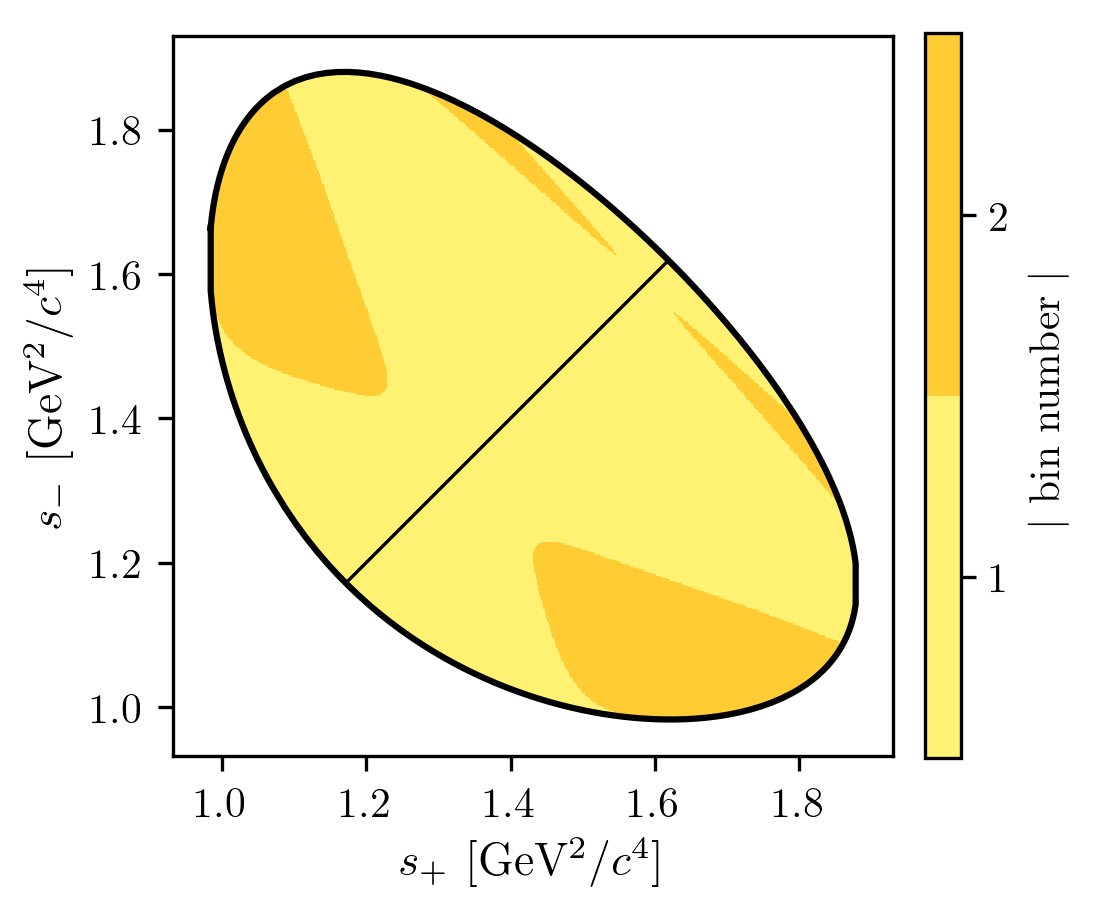
\includegraphics[height=5cm,valign=t]{figures/theory/binnings/KsKK_2bins.png}
        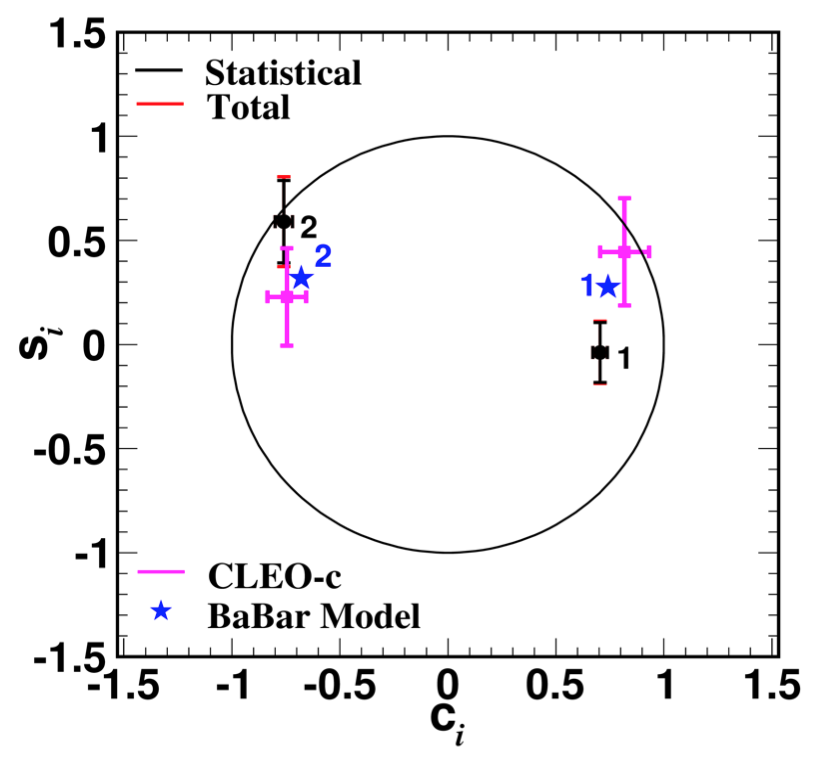
\includegraphics[height=4.8cm,valign=t]{figures/theory/bes_kskk_2bins.png}
        \caption{}
        \label{fig:kskk_bins_2}
    \end{subfigure}
    \begin{subfigure}{\columnwidth}
        \centering
        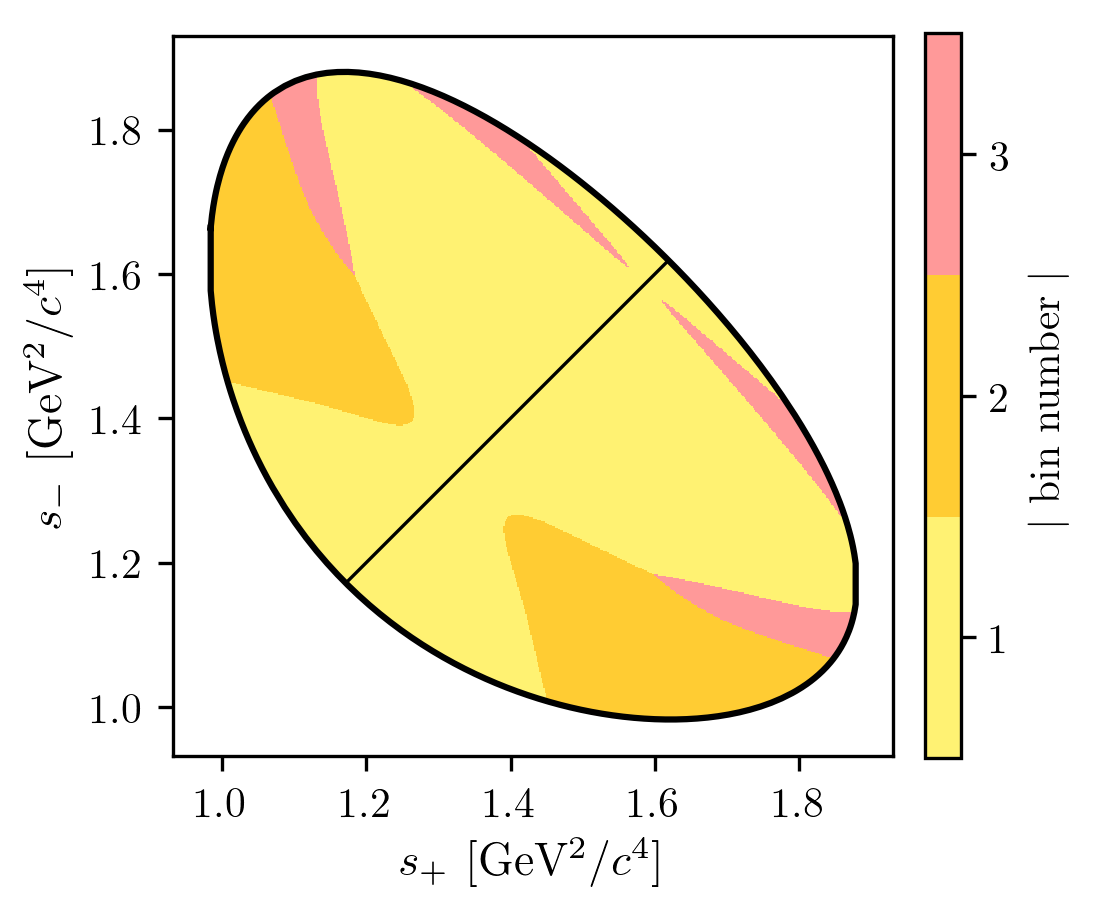
\includegraphics[height=5cm,valign=t]{figures/theory/binnings/KsKK_3bins.png}
        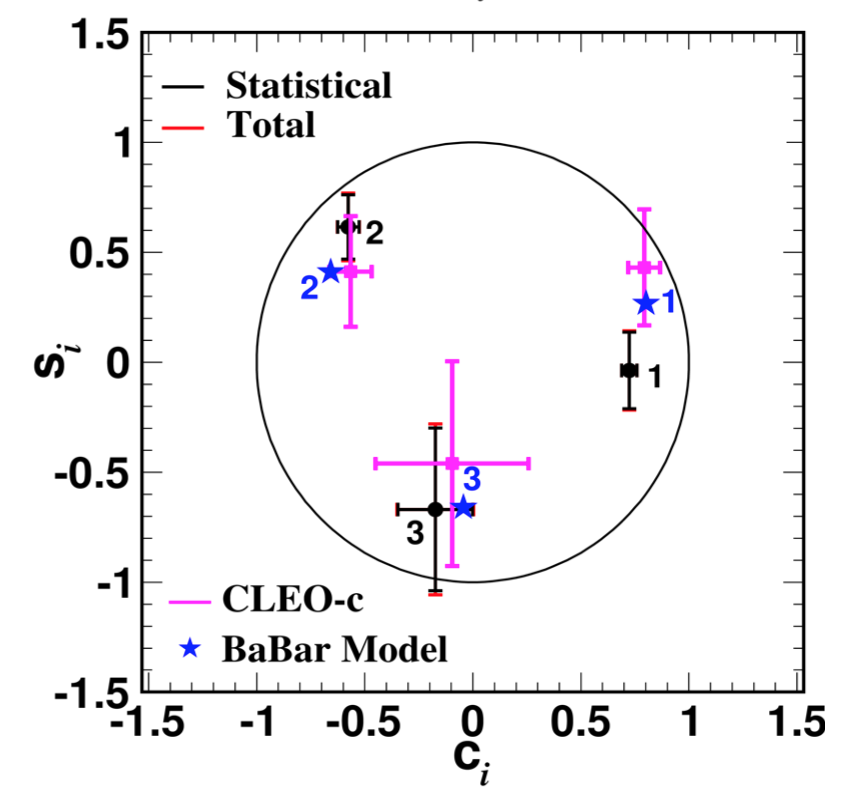
\includegraphics[height=4.8cm,valign=t]{figures/theory/bes_kskk_3bins.png}
        \caption{}
        \label{fig:kskk_bins_3}
    \end{subfigure}
    \begin{subfigure}{\columnwidth}
        \centering
        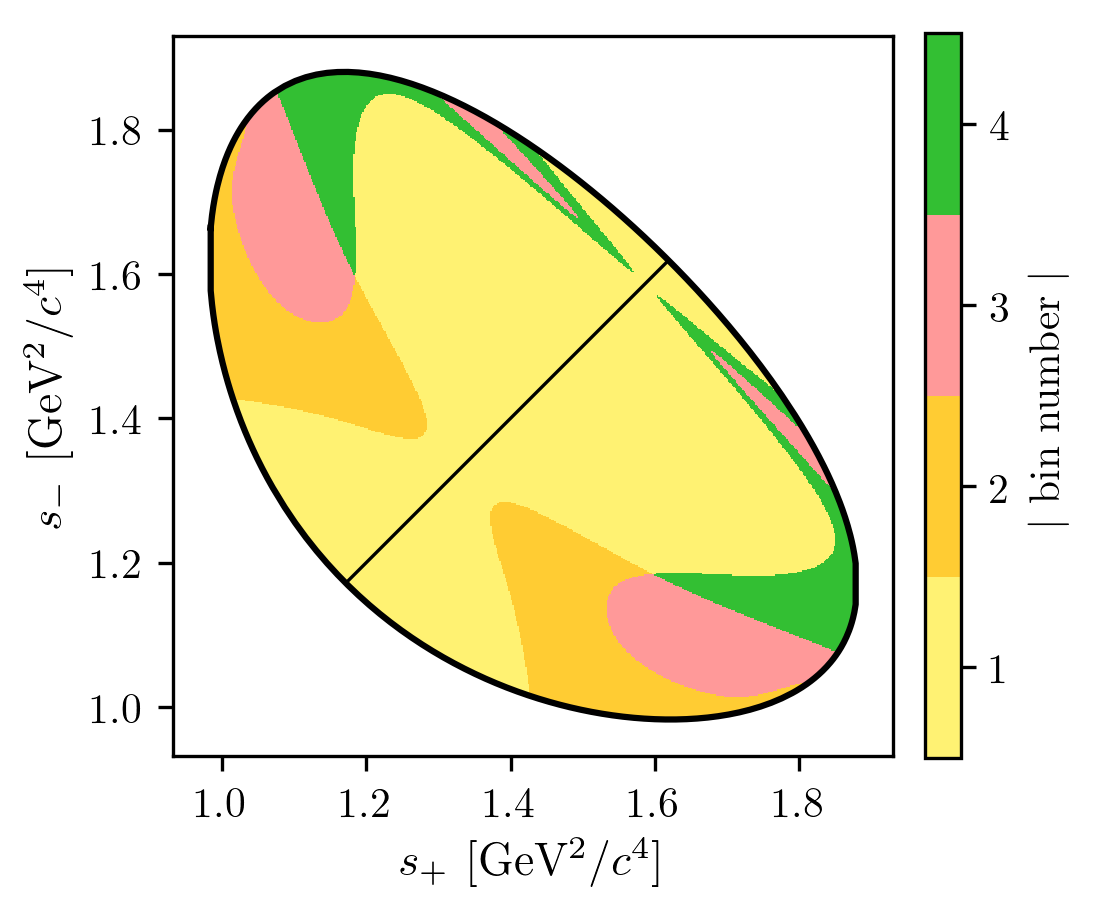
\includegraphics[height=5cm,valign=t]{figures/theory/binnings/KsKK_4bins.png}
        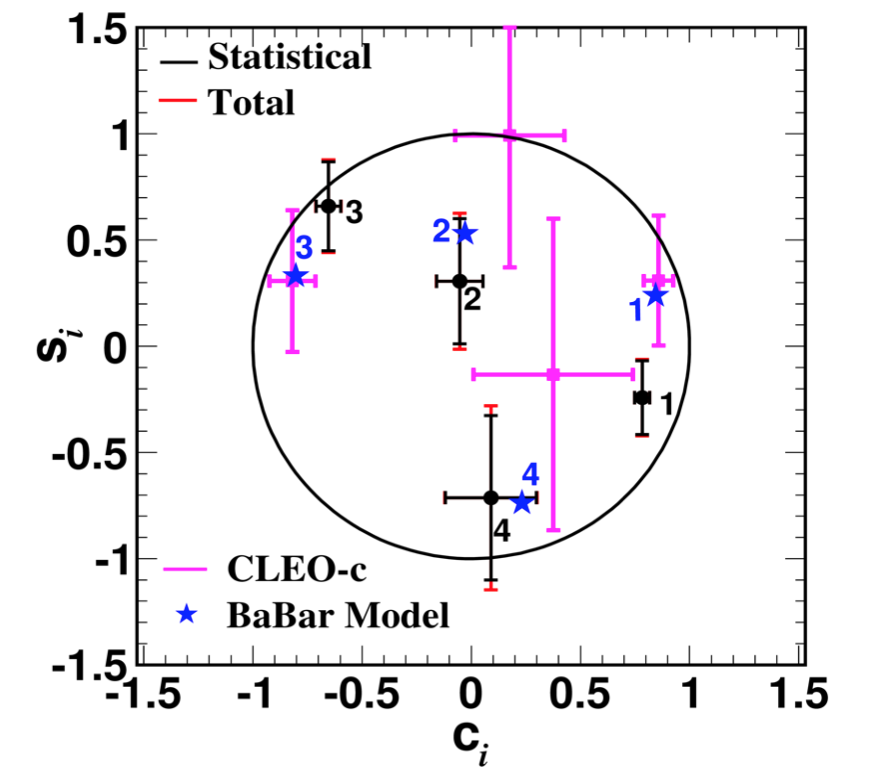
\includegraphics[height=4.8cm,valign=t]{figures/theory/bes_kskk_4bins.png}
        \caption{}
        \label{fig:kskk_bins_4}
    \end{subfigure}
    \caption{The (left) binning schemes and (right) measured values of $(\ci,\si)$ for the (a) 2-, (b) 3-, and (c) 4-bins binning schemes for \DtoKsKK decays. The plots of the measured values are taken from Ref.~\cite{BESCISIKSKK} and show the (error bars) results obtained by (black) BESIII, (pink) CLEO, and (blue) the model expectation using the model from Ref.~\cite{BABAR2010}.
    The measurement featured in this thesis uses the 2-bins scheme. Due to a different sign convention for the bin numbers, the \si values shown in the \besiii figures have the opposite sign to those defined in the text.}
    \label{fig:kskk_bins}
\end{figure}

% \begin{figure}[tb]
%     \centering
%     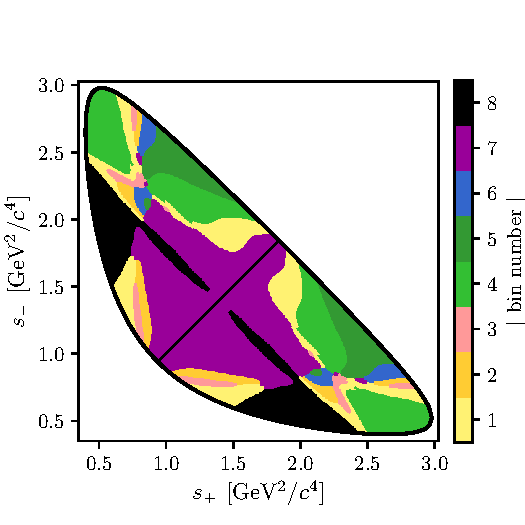
\includegraphics{figures/binning.pdf}
%     \caption{The \emph{optimal binning scheme} of the $\D\to\KS\pip\pim$ phase space~\cite{CLEOCISI}.}
%     \label{fig:optimal_binning_scheme}
% \end{figure}



% subsection a_model_independent_approach (end)

\subsection{Global CP asymmetry and the relation to GLW and ADS measurements} % (fold)
\label{sub:relation_to_glw_and_ads_measurements}



The introduction of separate normalisation factors $h^+$ and $h^-$ in Eq.~\eqref{eq:base_GGSZ_yields} hides the fact that information on $\gamma$ (in principle) can be obtained from the asymmetry in phase-space-integrated \Bp and \Bm yields. In the ideal case where $h^-=h^+$ the total yield asymmetry is 
\begin{align}\begin{split}\label{eq:A_GGSZ_global}
    A_{BPGGSZ} &= \frac{\sum_{i=-\mathcal N}^{\mathcal N} N^-_- - N^+_i}{\sum_{i=-\mathcal N}^{\mathcal N} N^-i- + N^+_i}
    = \frac{ \sum_{i=-\mathcal N}^{\mathcal N} \sqrt{K_iK_{-i}}c_i (x_- - x_+)}{1 + r_B^2 +2 \sum_{i=-\mathcal N}^{\mathcal N} \sqrt{K_iK_{-i}}c_i (x_- + x_+)} \\
    &=\frac{2 \sum_{i=1}^{\mathcal N} \sqrt{K_iK_{-i}}c_i (x_- - x_+)}{1 + r_B^2 +4 \sum_{i=1}^{\mathcal N} \sqrt{K_iK_{-i}}c_i (x_- + x_+) },
\end{split}\end{align}
using that $\sum_{i=-\mathcal N}^{\mathcal N} \sqrt{K_iK_{-i}}s_i=0$ by definition. The size of the asymmetry is governed by the factor $2\sum_{i=1}^{\mathcal N} \sqrt{K_iK_{-i}}c_i$, which is small for ${\D\to\KS\pip\pim}$ and ${\D\to\KS\Kp\Km}$ decays. The underlying reason is that $\delta_D(\sm, \sp)$ varies significantly across phase-space for these decays, as evident by the spread in the values of $c_i$ in Table~\ref{tab:cisi}, which reduces the \emph{average} of the asymmetry-generating \Dz--\Dzb interference term to being close to zero. The value of $2\sum_{i=1}^{\mathcal N} \sqrt{K_iK_{-i}}c_i$ is closely related to the \CP content of the final state in question: for a self-conjugate \CP even (odd) final state the \Dz and \Dzb decay amplitudes satisfy
\begin{align}
    {A_\Dz(\sm, \sp)=\varpm A_\Dzb(\sm, \sp)=\varpm A_\Dz(\sp, \sm)},
\end{align}
 meaning that $K_i=K_{-i}$ and $c_i=\pm1$; thus $2\sum_{i=1}^{\mathcal N} \sqrt{K_iK_{-i}}c_i= \varpm 1$. This motivates the definition of the \CP-even fraction of the decay
\begin{align}\label{eq:Fplus_global}
    \mathcal F_+ \equiv \frac{1}{2}\left(1 + 2\sum_{i=1}^{\mathcal N} \sqrt{K_i K_{-i}}c_i\right),
\end{align}
equivalent to the definition in Ref.~\cite{nayakFirstDeterminationCP2015} for the case $\mathcal N=1$.  With $\mathcal F_+$ in hand, the asymmetry in Eq.~\eqref{eq:A_GGSZ_global} can be rewritten
\begin{align}
    A_{BPGGSZ} &= \frac{(2\mathcal F_+-1) r_B \sin \delta_B \sin \gamma}{1 + r_B^2 (2\mathcal F_+-1) 2 r_B \cos \delta_B \cos \gamma},
\end{align}
which is the usual form used in quasi-GLW measurements~\cite{nayakFirstDeterminationCP2015,maldeFirstDeterminationCP2015}. The value of $\mathcal F_+$ is independent of the number and shape of bins in a given binning scheme, as long as the bin definitions follow the symmetry principles outlined in Section~\ref{sub:a_model_independent_approach}. 
For ${\D\to\KS\pip\pim}$ and $\DtoKskk$ decays the values of $\mathcal F_+$ are
\begin{align}
\begin{split}
    \mathcal F_+(\KS\pip\pim) = 57\,\% \\
    \mathcal F_+(\KS\Kp\Km) = 51\,\%
\end{split}
\end{align}
as evaluated with the Belle 2018 model~\cite{Belle2018} for ${\D\to\KS\pip\pim}$ decays and the BaBar 2010 model~\cite{BABAR2010} for $\D\to\KS\Kp\Km$ decays. In \BtoDK decays $r_B^{DK}\sim 0.1$, and the predicted global asymmetries are thus approximately 1--2\,\%, which is not resolvable with the current experimental yields. As shown in Chapter~\ref{ch:4-KS-CPV}, \CP violation in the \KS sector leads to asymmetries of a similar size, further complicating the use of global asymmetries to constrain \xpm and \ypm. Thus these modes are ill-suited for quasi-GLW measurements, and ignoring global asymmetries leads to a negligible loss of information on $\gamma$ in a BPGGSZ measurement. The reverse is true for a well-suited quasi-GLW mode, such as $\D\to\pip\pim\piz$: if $\mathcal F_+$ is close to either zero or unity, it means that $(c_i, s_i)$ will be close to $(\pm1, 0)$ in all bins for \emph{any} given binning scheme, and the set of bins will provide almost identical constraints on \xpm and \ypm. Thus, the binning of phase space leads to no significant gain in precision compared to a global analysis.


Indeed, a crucial quality of the BPGGSZ method, is that exactly because each bin-pair provides independent constraints on \xpm and \ypm, the method provides a single solution for $(\gamma, r_B, \delta_B)$ that does not suffer the ambiguities of the ADS and GLW approaches. In order to illustrate this further, it is useful to make one more comparison of the model-independent BPGGSZ formalism to the ADS and GLW formalisms. In a \CP symmetric world, the \Bp yield in bin $+i$ would equal the \Bm yield in bin $-i$. Therefore the relevant \CP asymmetry for a given Dalitz bin is
\begin{align}
\begin{split}\label{eq:Ai_definition}
        A_{BPGGSZ}^i &\equiv \frac{N^-_i - N^+_{-i}}{N^-_i + N^+_{-i}} \\
    &= \frac{\sqrt{K_i K_{-i}}(c_i(\xm-\xp)+s_i(\ym-\yp))}{K_i+r_B^2K_{-i} + 2 \sqrt{K_i K_{-i}}(c_i(\xm+\xp)+s_i(\ym+\yp))}.
\end{split}
\end{align}
This expression is identical to the ADS asymmetry in Eq.~\eqref{eq:ADS_asym} if the effective \D-decay parameters $r_D^i$ and $\delta_D^i$ are defined via
\begin{align}
    \kappa_i\cos\delta_D^i \equiv c_i \qquad, \qquad \kappa_i\sin \delta_D^i \equiv s_i \qquad, \qquad r_D^i \equiv \sqrt{K_i/K_{-i}},
\end{align}
and a coherence factor, $\kappa$, is included in the interference terms of the ADS expression, as is standard for multi-body \D decays~\cite{gronauImprovingBoundsGamma2003}. These parameters allow us to classify a given pair of bins with number $\pm i$ as either \emph{GLW-like}, if $ \delta_D^i$ is close to $0$ or $\pi$ and $r_D^i$  is close to unity, or \emph{ADS-like} if $r_D^i \ll 1$. The \CP-even fraction of the \D-decay can also be defined for a given bin-pair:
\begin{align}
\begin{split}
    \mathcal F_{+}^i = \mathcal F_+^{-i} &\equiv \frac{1}{2}\left(1 + 2c_i \frac{\sqrt{K_i K_{-i}}}{K_i + K_{-i}}\right) = \frac{1}{2}\left(1 + 2c_i \frac{r_D^i}{1+{r_D^i}^2}\right).
\end{split}
\end{align}
A GLW-even-like bin pair will have $\mathcal F_{+}^i\simeq 1$ and a GLW-odd-like bin pair will have $\mathcal F_{+}^i\simeq 0$.

Table~\ref{tab:bin_categories} summarises a classification of the bins for the optimal $\DtoKspipi$ binning scheme and the 2-bins ${\DtoKskk}$ binning scheme following these principles. Two bin pairs are classified as \emph{Odd-even}; in these bins, $r_D^i$ is not particularly small but $\mathcal F_+^i$ is close to 0.5. The name refers to the that fact that for these bins $A_{BPGGSZ}^i$, as defined in Eq~\eqref{eq:Ai_definition}, will be positive and $A_{BPGGSZ}^{-i}$ negative (or vice versa). The fact that multiple bin types appear for both the \DtoKspipi and \DtoKsKK modes underline that each mode benefits from being analysed in the BPGGSZ formalism. 

\begin{table}
    \centering
    \caption{Classification of the bins used in model-independent GGSZ measurements, in terms of whether the interplay between the \Dz and \Dzb amplitudes in the bin resemble typical GLW or ADS behaviour. The parameters are calculated using the 2018~Belle~model~\cite{} for \DtoKspipi decays and the 2010~BaBar~model~\cite{} for \DtoKsKK decays.
    \label{tab:bin_categories}
    }
    \begin{tabular}{cccccc}
    \toprule
    \multicolumn{5}{c}{Optimal binning scheme: $\DtoKspipi$} \\
    \midrule
    Bin $i$ & $\hat r_D$ & $\hat \delta_D$ & $\mathcal F_+$ & $\kappa$ & Bin type \\
    \midrule
% autogenerated with thesis_notebooks/02_Theory/BinCategories.ipynb
    1 & $0.473$ & $    91.9^\circ$ & $48.97\,\%$ & 0.81 & Odd-even \\
    2 & $0.164$ & $    11.1^\circ$ & $63.38\,\%$ & 0.85 & ADS-like \\
    3 & $0.157$ & $    79.4^\circ$ & $52.50\,\%$ & 0.89 & ADS-like \\
    4 & $0.768$ & $   175.3^\circ$ & $5.85\,\%$ & 0.92 & GLW-odd-like \\
    5 & $0.759$ & $   -99.9^\circ$ & $42.84\,\%$ & 0.87 & Odd-even \\
    6 & $0.223$ & $   -64.5^\circ$ & $57.92\,\%$ & 0.87 & ADS-like \\
    7 & $0.651$ & $   -13.3^\circ$ & $89.44\,\%$ & 0.89 & GLW-even-like \\
    8 & $1.745$ & $    21.0^\circ$ & $87.08\,\%$ & 0.92 & GLW-even-like \\
    \midrule \\
    \midrule
    \multicolumn{5}{c}{2-bins binning scheme: $\DtoKskk$} \\
    \midrule
    Bin $i$ & $\hat r_D$ & $\hat \delta_D$ & $\mathcal F_+$ & $\kappa$ & Bin type \\
    \midrule
    % autogenerated with thesis_notebooks/02_Theory/BinCategories.ipynb
    1 & $0.816$ & $    19.8^\circ$ & $86.14\,\%$ & 0.78 & GLW-even-like \\
    2 & $0.775$ & $   154.5^\circ$ & $16.23\,\%$ & 0.77 & GLW-odd-like \\

    \bottomrule
    \end{tabular}
\end{table}

% subsection relation_to_glw_and_ads_measurements (end)




\section{Strategy for the LHCb measurement} % (fold)
\label{sec:strategy_for_lhcb_measurement}

The main topic of the thesis is a model-independent BPGGSZ measurement using $\BtoDK$ and $\BtoDpi$ decays, with two \D final states $\KS\pip\pim$ and $\KS\Kp\Km$. The measurement is based on the data collected by the \lhcb experiment, described in detail in next chapter, during Run~1~and~2 of the Large Hadron Collider. The optimal binning scheme is used for the ${\DtoKspipi}$ mode, with the combined strong-phase inputs from the BESIII~\cite{BESCISI} and CLEO~\cite{CLEOCISI} collaborations published in Ref.~\cite{BESCISI}. For the \DtoKsKK channel, the 2-bins scheme is used, again using a combination~\cite{BESCISIKSKK} of measurements from the CLEO~\cite{CLEOCISI} and \besiii~\cite{BESCISIKSKK} collaborations. The details of the analysis are presented in Chapter~\ref{ch:5-GGSZ-measurement}, but the overall strategy, and a few extensions of the formalism from the previous sections, are given here.

It is the first time that $\gamma$ is measured in \BtoDpi decays with the BPGGSZ method at \lhcb (although it has been used as a control channel in previous measurements with \BtoDK decays~\cite{LHCb-PAPER-2012-027,LHCb-PAPER-2014-041,LHCb-PAPER-2018-017}). The promotion of \BtoDpi to a signal channel has two benefits. First of all, there is a small degree of \CP violation in \BtoDpi decays, and therefore a measurement of \CP observables in \BtoDpi decays does provide some further information on $\gamma$. However, the latest \lhcb combinations have generally \emph{not} included this information, because the currently measured \BtoDpi observables allow for two solutions for $(r_B^{\D\pi}, \delta_B^{\D\pi})$~\cite{LHCb-PAPER-2016-032}. One of these is almost certainly non-physical, and the presence of both makes the statistical interpretation of the results on $\gamma$ highly non-trivial. The multiple solutions arise because the constraints on the \BtoDpi parameters come from ADS/GLW measurements. As described in Section~\ref{sec:constraints_on_gamma}, the situation is resolved by the measurement presented in the thesis, and therefore \BtoDpi measurements can be included without incurring such problems in the future. However, the \BtoDpi channel constrains $\gamma$ much less than the \BtoDK channel, and therefore the impact on the overall precision is small. The second, more significant, benefit from the promotion of \BtoDpi to a signal channel, is that the analysis avoids a significant systematic uncertainty due \lhcb acceptance effects that was present in earlier analyses. This is described further below.

\begin{figure}[tbp]
    \centering
    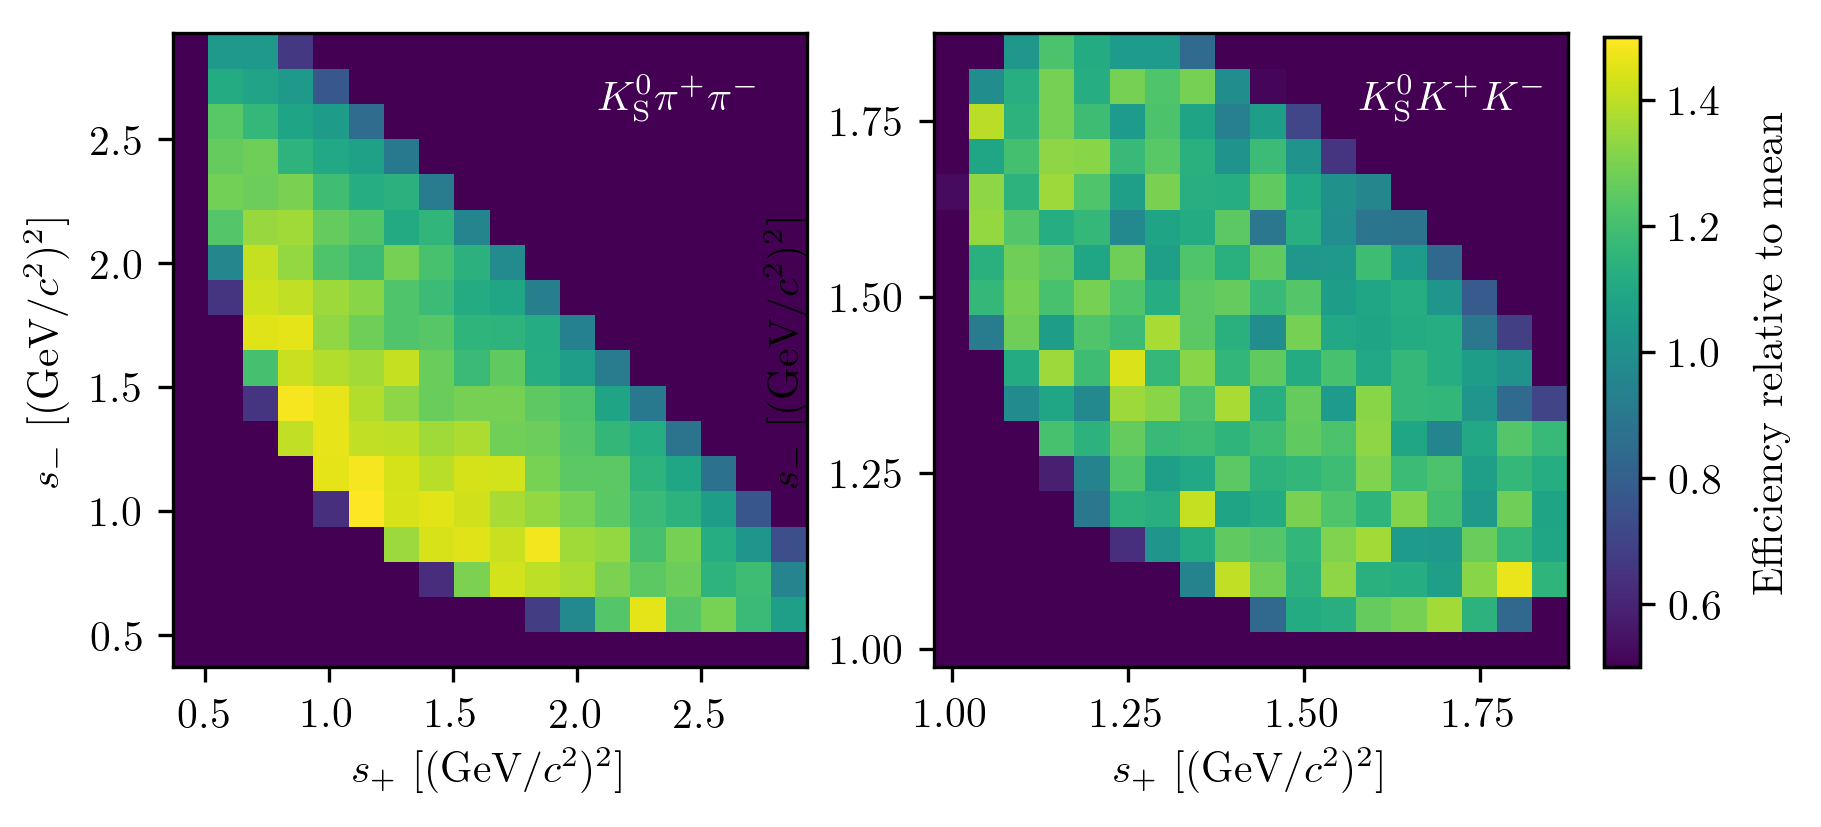
\includegraphics[width=\columnwidth]{figures/analysis/DP_thesis_profile_PiPi_and_KK_KK.png}
    \caption{The \lhcb acceptance in simulated \BtoDK decays where (left) ${\DtoKspipi}$ and (right) ${\DtoKsKK}$.}
    \label{fig:DP_profile}
\end{figure}

Due to the geometry of the \lhcb detector, the signal reconstruction efficiency for $\Bpm\to\D(\to\KS h^+h^-)h'^\pm$ decays varies significantly across the \D-decay phase space. This is clearly visible in Fig.~\ref{fig:DP_profile}, where examples of the acceptance profile for  $\Bpm\to\D(\to\KS h^+h^-)\Kpm$ decays in \lhcb simulation are shown, and the acceptance is seen to vary $\pm50\,\%$ relative to the average over the allowed phase space. The main feature, especially visible for \DtoKspipi decays, is a falling acceptance along the diagonal of the Dalitz plot, which is caused by the fact that a non-significant fraction of \KS mesons escape the \lhcb tracking region before decaying, and that there is a correlation between $m^2(h^+h^-)$ and the \KS momentum in the \lhcb frame. The non-uniform acceptance results in yield equations that differ slightly from those derived in the preceding sections. Denoting the efficiency profile as $\eta(\sm, \sp)$, the expressions in Eq.~\eqref{eq:base_GGSZ_yields} are modified to
\begin{align}
\begin{split}    \label{eq:lhcb_GGSZ_yields}
    N^-_i = h^\Bm \left[\Fi + \rB^2\Fmi + 2\sqrt{\Fi\Fmi}\left(\ci'\xm+\si'\ym\right)\right], \\
    N^+_i = h^\Bp \left[\Fmi + \rB^2\Fi + 2\sqrt{\Fi\Fmi}\left(\ci'\xp-\si'\yp\right)\right],
\end{split}
\end{align}
where the phase-space integrated quantities now include the efficiency profile
\begin{align}\label{eq:Fi_def}
    F_i &= \frac{1}{N_F}\int_i\text{d}s^2 \,\eta(\smp)|\ADS(\smp)|^2, &
    N_F &=\int\text{d}s^2 \,\eta(\smp)|\ADS(\smp)|^2,
\end{align}
\begin{align}\label{eq:ci_si_with_eff}
\begin{split}
    \ci' &= \frac
    {\int_i \text{d}s^2 \,\eta(\smp)|\ADS(\smp)||\ADS(\spm)|\cos[\delta_D(\smp)]}
    {\sqrt{\int_i \text{d}s^2 \,\eta(\smp)|\ADS(\smp)|^2}\sqrt{\int_i \text{d}s^2 \,\eta(\smp)|\ADS(\spm)|^2}},
\end{split}
\end{align}
with an analogous definition of $\si'$. At leading order, the strong-phase parameters are unaffected by the non-uniform efficiency, and, in addition, the bin definitions favour bins for which $\cos[\delta_D(\smp)]$ and $\sin[\delta_D(\smp)]$ are approximately constant across each bin.  Therefore, the  \ci and \si values reported by the charm factories are used directly in the measurement. The impact on the obtained central values is negligible, as described in detail in Section~\ref{sec:systematic_uncertainties} where a systematic uncertainty is assigned. 

The \Fi and $K_i$ parameters \emph{are} significantly different, because the experimental acceptance profile in \lhcb is significantly non-uniform.  Given external inputs for the strong-phase parameters, it is possible to fit the \Fi parameters \emph{and} $\xpm$ and $\ypm$ simultaneously in a fit to the \lhcb \BtoDK data set, in which case the obtained \Fi parameters incorporate the correct acceptance profile correction by construction. However, the obtainable precision for the \CP observables measured by this procedure is suboptimal. As an alternative, the first \lhcb measurement~\cite{LHCb-PAPER-2012-027} determined acceptance-related yield corrections based on model predictions of \Ki, adjusted using the relative acceptance between bins determined in \BtoDpi decays (assuming \CP symmetry and that the \Ki were correctly predicted by the model). 
%Since the \Fi parameters relate to the \D decay, they can effectively be obtained in the \BtoDpi sample  and used in the \BtoDK channel. 
However, there is \CP violation present in the \BtoDpi decays, which led to a dominant systematic uncertainty. Later \lhcb measurements~\cite{LHCb-PAPER-2014-041,LHCb-PAPER-2018-017} instead relied on flavour tagged \D mesons from $\Bzb\to\Dstarp(\to \Dz \pip)\mu^- \bar \nu_\mu X$ decays to obtain \Fi, where no \CP violation is possible. However, due to necessarily different triggering paths and selections, the acceptance profile is not exactly identical between semi-leptonic decays and the \BtoDh decays of interest. An efficiency correction based on (very large) samples of simulated decays was therefore applied to obtain the correct \Fi, and in this case,  the uncertainty related to the correction constituted the largest systematic uncertainty on the measurement.

Both sources of systematic uncertainty can be avoided by making a simultaneous analysis of \BtoDK and \BtoDpi decays, where \CP-violating observables are measured in \emph{both} channels and the \Fi parameters are shared. It is a reasonable assumption that $F_i^{DK}=F_i^{D\pi}$ to a very good approximation, given the similar kinematics of the decays. The assumption is confirmed using simulated decays in Section~\ref{sub:efficiency_profile_over_the_dalitz_plot}, for the candidate selection used in the measurement of the thesis. Effectively, the \Fi are determined in the high statistics \BtoDpi channel, but with no systematic effect from \CP-violation in that channel, since the \CP-violation is incorporated in the yield description. 

At the start of the work that lead to this thesis, it was not clear to what degree the measured \CP-violating observables in \BtoDpi decays were affected by \CP violation in the neutral kaon sector. The potential bias had been shown to be $\sim1^\circ$ in the \BtoDK channel, a negligible effect given the past precision, but to scale with $1/r_B$~\cite{grossmanEffectsBarMixing2014} suggesting potentially large biases in the \BtoDpi channel where $r_B$ is $\sim20$ times smaller. However, the dedicated analysis presented in Chapter~\ref{ch:4-KS-CPV} has proved the effect to be an order of magnitude smaller in BPGGSZ measurements than suggested in Ref~\cite{grossmanEffectsBarMixing2014}, and the simultaneous measurement is indeed viable. 

The measurement is performed by making extended maximum-likelihood fits to the $m_B$ spectra of $\B\to\D(\to\KS h^+h^-)h'^\pm$ candidates split by charge and Dalitz bin. The \BtoDK signal yields are parameterised using the expressions in Eq.~\eqref{eq:lhcb_GGSZ_yields} directly, and the fit therefore determines values for \xpmdk and \ypmdk. The Cartesian \CP-violating observables \xpm and \ypm are employed because they lead to better statistical behaviour than fits to data where the underlying parameters $(\gamma, r_B^{DK}, \delta_B^{DK})$ are determined directly, at the cost of introducing a fourth degree of freedom. With the addition of the \BtoDpi mode as a true signal channel, two new underlying parameters are introduced, $r_B^{\D\pi}$ and $\delta_B^{\D\pi}$. There is a choice to be made, in terms of how to define the observables that are measured. One is to introduce an additional set of four observables, $(x_-^{D\pi}, y_-^{D\pi}, x_+^{D\pi}, y_+^{D\pi})$, that are analogous to the \BtoDK parameters. As an alternative, it is possible to introduce only two Cartesian parameters~\cite{Tico:2018qmg,JordiXi2}, by defining
\begin{subequations}
\begin{align}
    \xi^{\D\pi} = \left(\frac{r_B^{\D\pi}}{r_B^{DK}}\right)\exp [i (\delta_B^{\D\pi}-\delta_B^{DK})]
\end{align}
and letting
\begin{align}
    \xxidpi &= \Re [\xi^{\D\pi}] & \yxidpi &= \Im [\xi^{\D\pi}].
\end{align}
\end{subequations}
In terms of these parameters, the usual Cartesian \xpm and \ypm are given by
\begin{align}\label{eq:xy_from_xi}
    x_\pm^{\D\pi} &= x_\xi^{\D\pi}x_\pm^{DK} - y_\xi^{\D\pi}y_\pm^{DK}, 
    & y_\pm^{\D\pi} &= x_\xi^{\D\pi}y_\pm^{DK} + y_\xi^{\D\pi}x_\pm^{DK}.
\end{align} 
Using this expression, the \BtoDpi yields can also be defined via Eq.~\eqref{eq:lhcb_GGSZ_yields} in the maximum-likelihood fit. Note that $\xi$ does not depend on $\gamma$: all information on \CP asymmetries in both the \BtoDK and \BtoDpi channels is encoded in \xpmdk and \ypmdk. In the thesis, the latter parameterisation is chosen, because it allows for a stable fit for all six $x$ and $y$ parameters and the shared \Fi; the choice is described in much greater detail in Section~\ref{sub:fit_setup}. 

The combined analysis of \BtoDK and \BtoDpi decays presents a significant step forward, because it solves the problem of obtaining \Fi parameters for the appropriate acceptance profile in a manner that avoids leading systematic uncertainties, and almost all reliance on simulation. This is of great importance, if the large data samples that will be collected by \lhcb in the future are to be exploited to their full potential.


% subsection measuring_strong_phase_inputs_at_charm_factories (end)


% subsection extending_the_method_to_multiple_decay_channels (end)

% section the_ggsz_method(end)

% section cp_violation_in_the_standard_model (end)
% \begin{savequote}[8cm]
% Alles Gescheite ist schon gedacht worden.\\
% Man muss nur versuchen, es noch einmal zu denken.

% All intelligent thoughts have already been thought;\\
% what is necessary is only to try to think them again.
%   \qauthor{--- Johann Wolfgang von Goethe \cite{von_goethe_wilhelm_1829}}
% \end{savequote}

\chapter{The \lhcb experiment}
\label{ch:3-detector}


The \lhcb experiment is one of the four large experiments at the Large Hadron Collider (LHC), the World's most powerful accelerator, able to accelerate protons to record centre-of-mass energies of $\sqrt{s}=13\tev$ in a 27\km long tunnel underneath Geneva. The \lhcb experiment is specifically designed to study the large number of particles containing $b$ or $c$ quarks produced in such collisions, which has led to a number of design decisions that make the \lhcb unique among the \lhcb experiments. The \lhcb is not a solid-angle detector like the other three LHC experiments, CMS, ATLAS, and ALICE, but a single-arm spectrometer, instrumented in the forward region where the majority of $b\bar b$ pairs are produced. During data-taking the experiment is operated at a lower instantaneous luminosity than the other experiments, leading to far fewer $pp$ interactions. This, in combination with a vertex detector located extremely close to the interaction point, allows for excellent resolution in the reconstruction of primary and secondary vertex locations, crucial to many of the central measurements of the experiment. Finally, dedicated particle-identification detectors allow for very efficient separation of hadron species, absolutely crucial to isolate a number important signal decays (including the \BtoDK decay studied in the thesis). Each of these features is described in much greater detail in the sections below.



During operation of the LHC, bunches of about $\mathcal O(10^{11})$ protons are accelerated to the desired centre-of-mass energy in a series of linear and circular accelerators, the final one being the LHC itself. This is illustrated in Fig.~\ref{fig:CERN_accerators}. The bunches remain in the LHC for the duration of a \emph{fill}, typically about 12 hours, where they are made to collide at four distinct locations, the collision points, each home to one of the big experiments. The collisions occur with a frequency of up to 40\,MHz. A fill ends when the beams are dumped, typically because the average number of protons in the bunches has become too low, after which the whole process begins again.

\begin{figure}[tb]
    \centering
    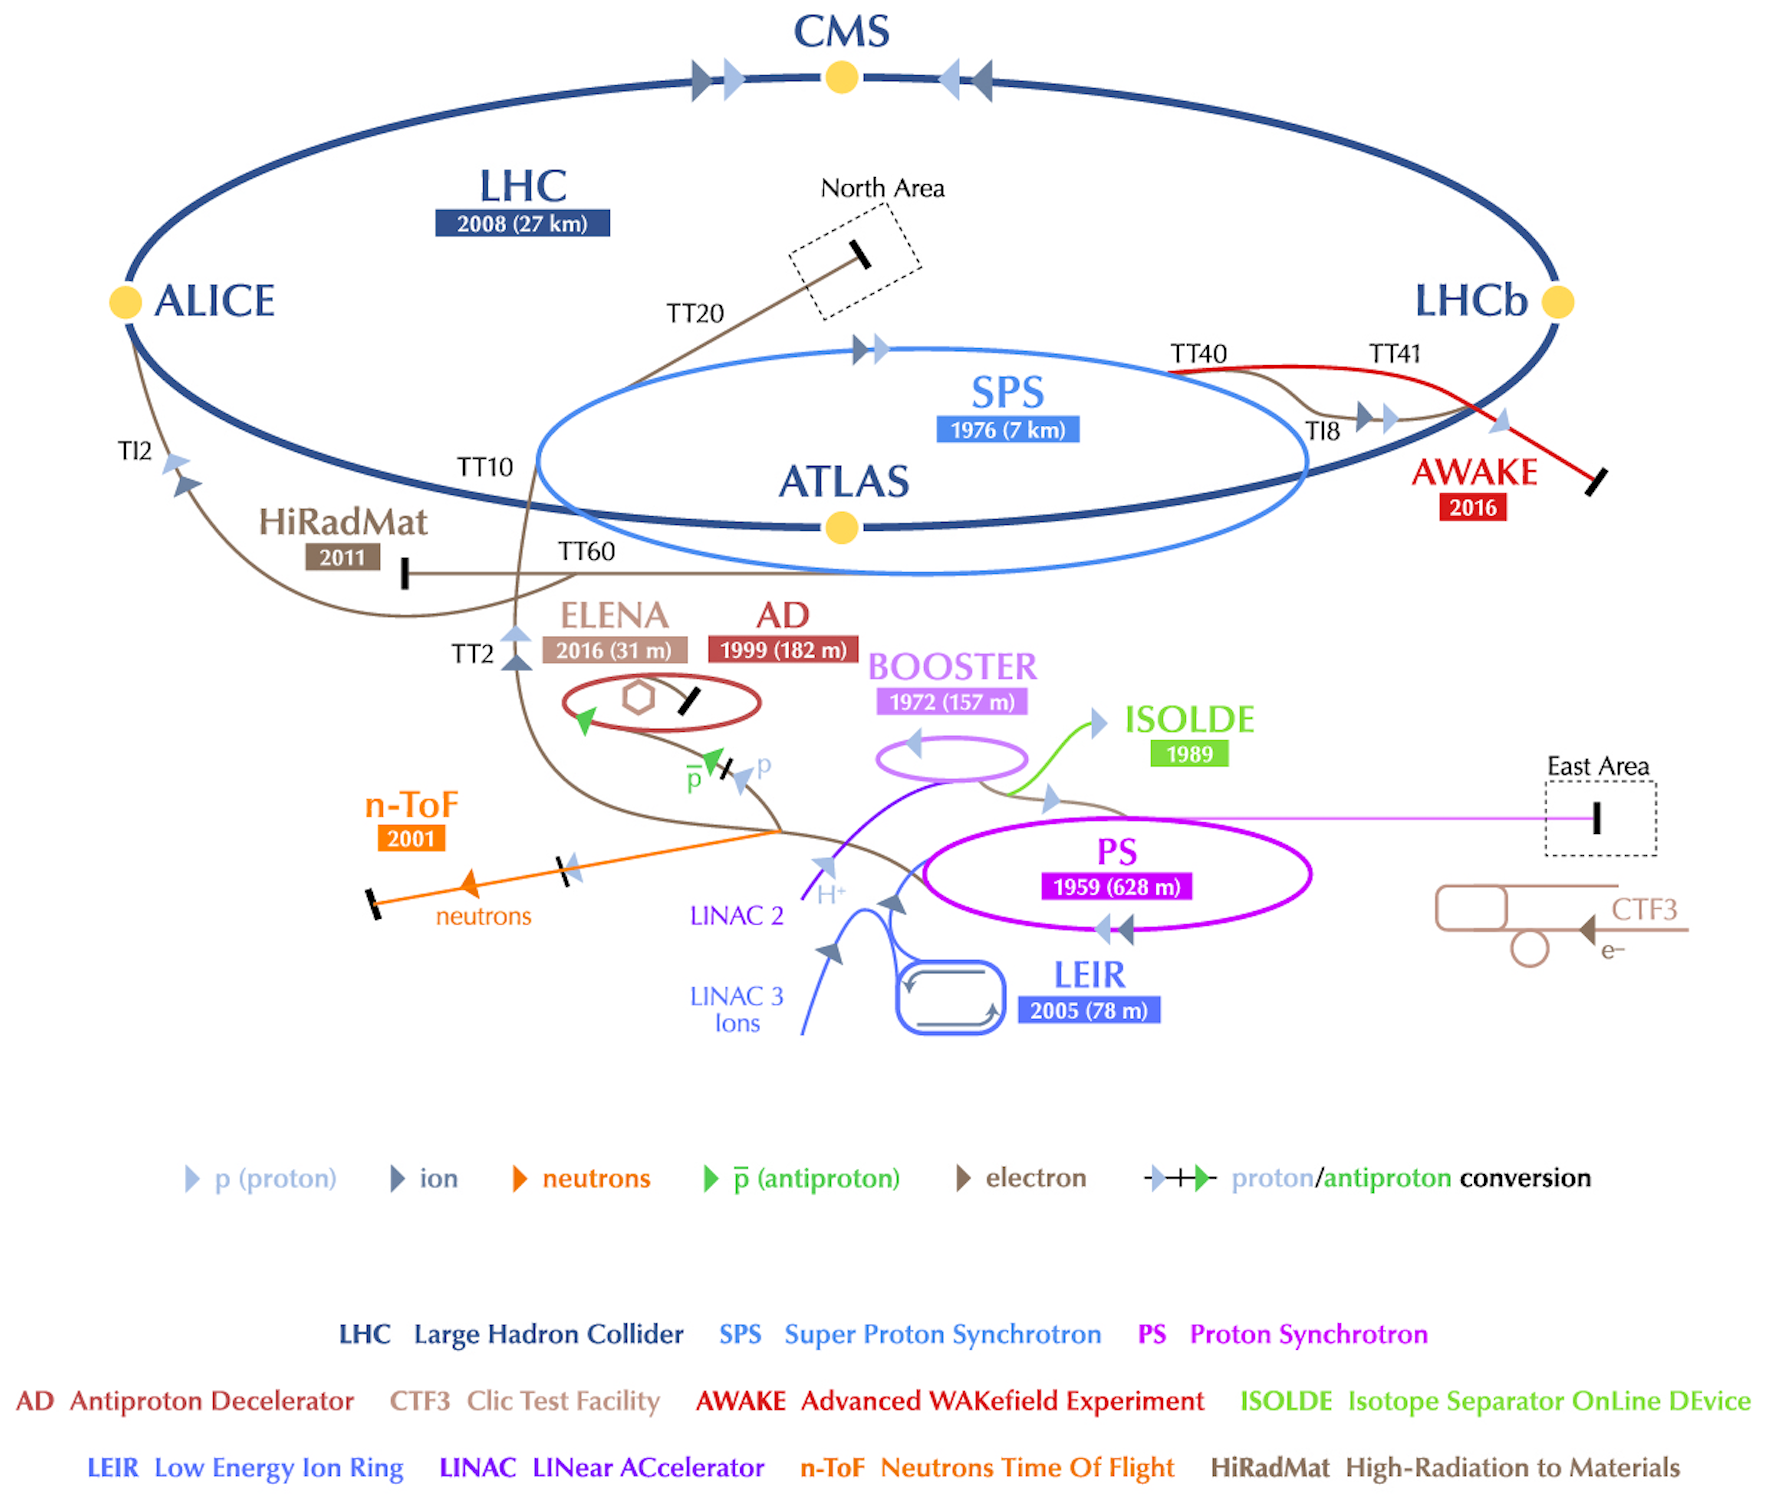
\includegraphics[width=0.9\columnwidth]{figures/detector/CERN_complex.png}
    \caption{The CERN accelerator complex, including the length and construction year for a number of accelerators, not all of which are used in $pp$ operations. During $pp$ operation, the proton acceleration chain is: LINAC 2 \to BOOSTER \to \PS \to SPS \to LHC.  The figure is reproduced from Ref.~\cite{CERNcomplex}.}
    \label{fig:CERN_accerators}
\end{figure}

The LHC has been providing $pp$ collisions during two periods so far: Run~1 during 2011 and 2012, where the centre-of mass energies were $\sqrt{s}=7\tev$ and $8\tev$ respectively, and Run~2 from 2015 to 2018, where $\sqrt{s}=13\tev$. The instantaneous luminosity at the \lhcb collision point has been $4\times 10^{32} \cm^{-2} \,\mathrm s^{-1}$, and has allowed for the collection of data set corresponding to a total of 3\invfb during Run~1 and 6\invfb during Run~2. The full data set forms the basis of the thesis. This instantaneous luminosity is significantly lower than at other collision points, for example the peak instantaneous luminosity in the ATLAS detector was about $20\times 10^{33}\cm^{-2}\,\mathrm s^{-1}$ in 2018~\cite{ATLAS-CONF-2019-021}, about 50 times higher than in \lhcb. The lower luminosity is necessary to limit the number of $pp$ interactions per bunch crossing to an average of about 1--1.6, necessary for a vertex reconstruction with the required precision. It is achieved by colliding the proton beams with a traverse off-set at the \lhcb collision point. This has the added benefit that the offset can be continuously adjusted during a fill of the LHC, and thus all data can be taken at the same instantaneous luminosity, allowing for simpler trigger configuration, and simpler subsequent analysis because the detector occupancy is constant. The lower luminosity, of course, comes with the downside that the collected data sample is smaller.

\begin{figure}[tb]
    \centering
    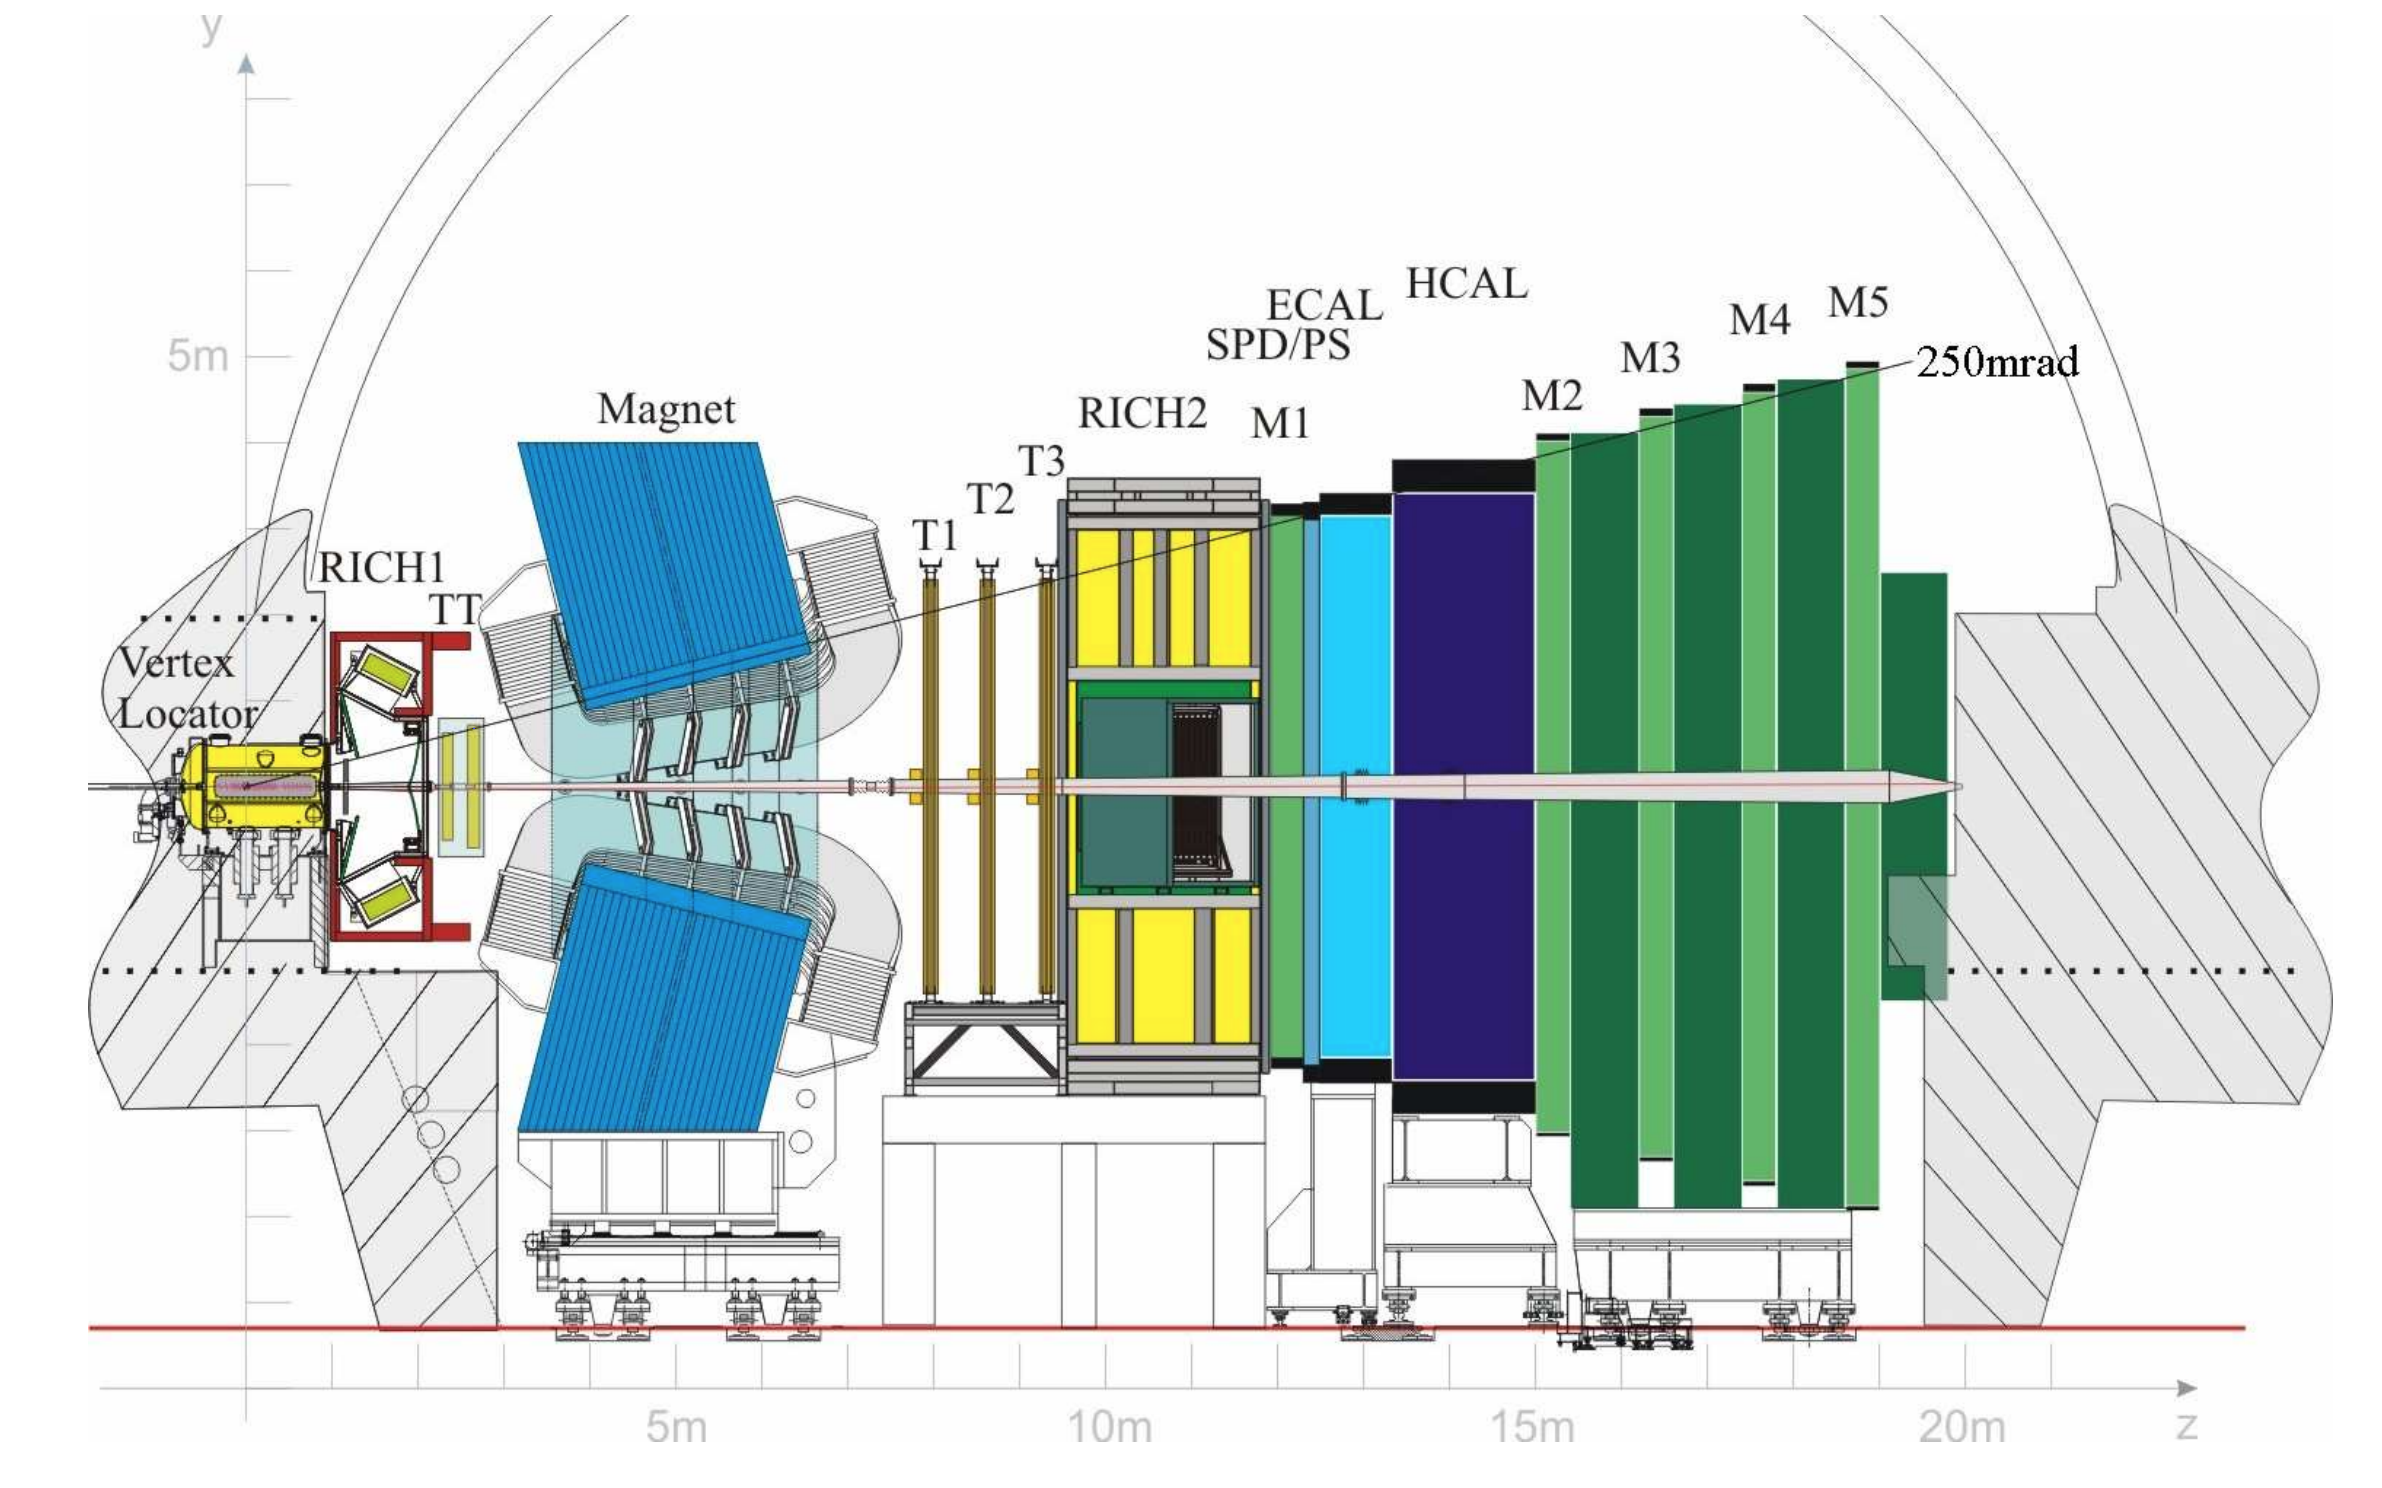
\includegraphics[width=\columnwidth]{figures/detector/LHCb_detector.png}
    \caption{Overview of the \lhcb detector reproduced from Ref.~\cite{LHCb-detector,CERN-LHCC-2003-030}. The individual sub detectors are described in detail in the chapter.}
    \label{fig:lhcb_detector}
\end{figure}



\section{The LHCb subdetectors} % (fold)
\label{sec:subdetectors}

\begin{figure}[tbp]
    \centering
    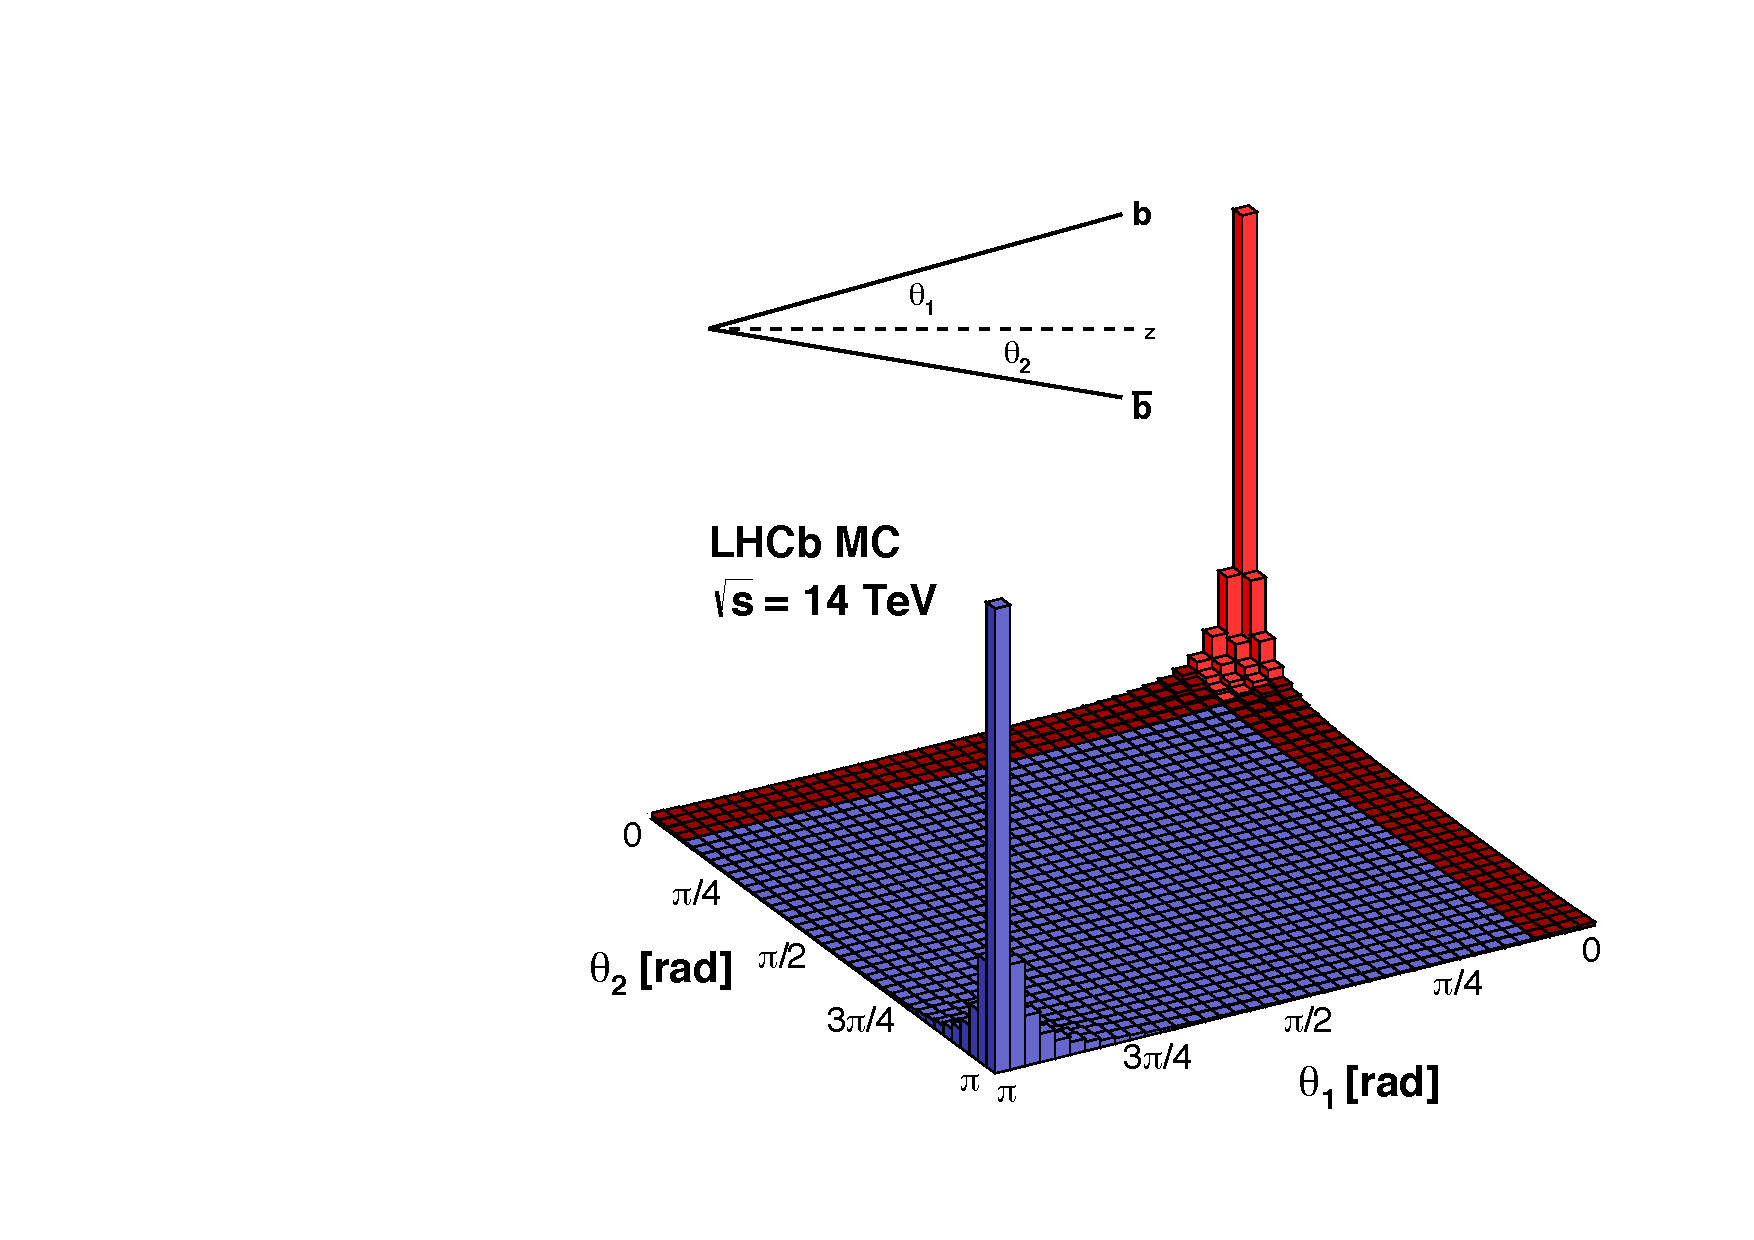
\includegraphics[width=0.8\columnwidth]{figures/detector/bbangles.pdf}
    \caption{Production cross section of $b\bar b$ pairs at a centre-of-mass energy of $\sqrt s = 14\tev$, as a function of $\theta_1$ and $\theta_2$, the angle of the $b$ and $\bar b$ quark, respectively, with respect to the beam axis $z$. The \lhcb acceptance is marked in red. The cross-section looks very similar for $\sqrt s = 7,\; 8\tev$. The figure is taken from Ref.~\cite{bbangles}.}
    \label{fig:bb_angles}
\end{figure}

The \lhcb detector, shown in Fig.~\ref{fig:lhcb_detector},  is able to detect particles in the forward region $\eta\in[2, 5]$, corresponding to an angle $\theta$ with respect to the beam line between 15 and $300/250$\,mrad in the horizontal/vertical direction. As illustrated in Fig.~\ref{fig:bb_angles}, the $b\bar b$ production cross section is very large within the \lhcb acceptance: even though the acceptance covers less than 2\,\% of the solid angle,  24\,\% of all $b\bar b$ pairs created at $\sqrt{s}=14\tev$ are within the acceptance. The detector is described with a coordinate system, where the $z$-axis is along the beam line and the $x$ $(y)$ axis is in the horizontal (vertical) directions normal to the beam line. The origin is at the collision point. The experiment consists of a number of sub detectors, located in the region from around the interaction point, and up to a distance of $z=20\,$m along the beam line (in the following, the direction from the interaction point towards the sub detectors is denoted \emph{downstream}, and the opposite direction \emph{upstream}). This section describes each of them in detail.
 
\subsection{The VELO} % (fold)
\label{sub:the_velo}
The VErtex LOcator (VELO)~\cite{VELO-TDR} is a silicon detector located immediately around the collision point, used to provide precise measurements of the particle track coordinates in the interaction region. These are used to reconstruct the production and decay vertices of beauty and charm hadrons with a very high accuracy, allowing for an accurate reconstruction of their life times, and for efficient background rejection. The ability to distinguish tracks originating in secondary vertices also plays a crucial role in efficient triggering, as described further below.

The detector consists of 21 VELO stations positioned along the beam line as illustrated in Fig.~\ref{fig:VELO_stations}. Each station consists of two \emph{modules}, mounted on each side of the beam line; each module, in turn, consists of two silicon strip detectors,  where the strips are oriented to provide a measurement of $r$, the radial distance from the beam line, and  $\phi$, the azimuthal angle, respectively. This is illustrated in Fig.~\ref{fig:VELO_sensors}. The strip pitch varies between 40 and $100\,\mu$m depending on the distance from the beam line.  The stations are positioned such that all tracks that are within the acceptance region of the downstream detectors and originate at the interaction point are guaranteed to intersect 3 detector segments. During operation, the segments are located only 8\mm from the beam; this is achieved by mounting them on a moving frame that can be retracted during beam commissioning to avoid radiation damage. The detectors are kept in a vacuum, shielded from the beam vacuum by a $0.3\mm$ thick \emph{RF foil} made of aluminium that also serves to screen the detector from electric fields induced by the proton beam. The silicon sensors were kept at an operating temperature of about -7\,C$^\circ$, achieved with a liquid-CO$_2$ cooling system.

\begin{figure}[tbp]
    \centering
    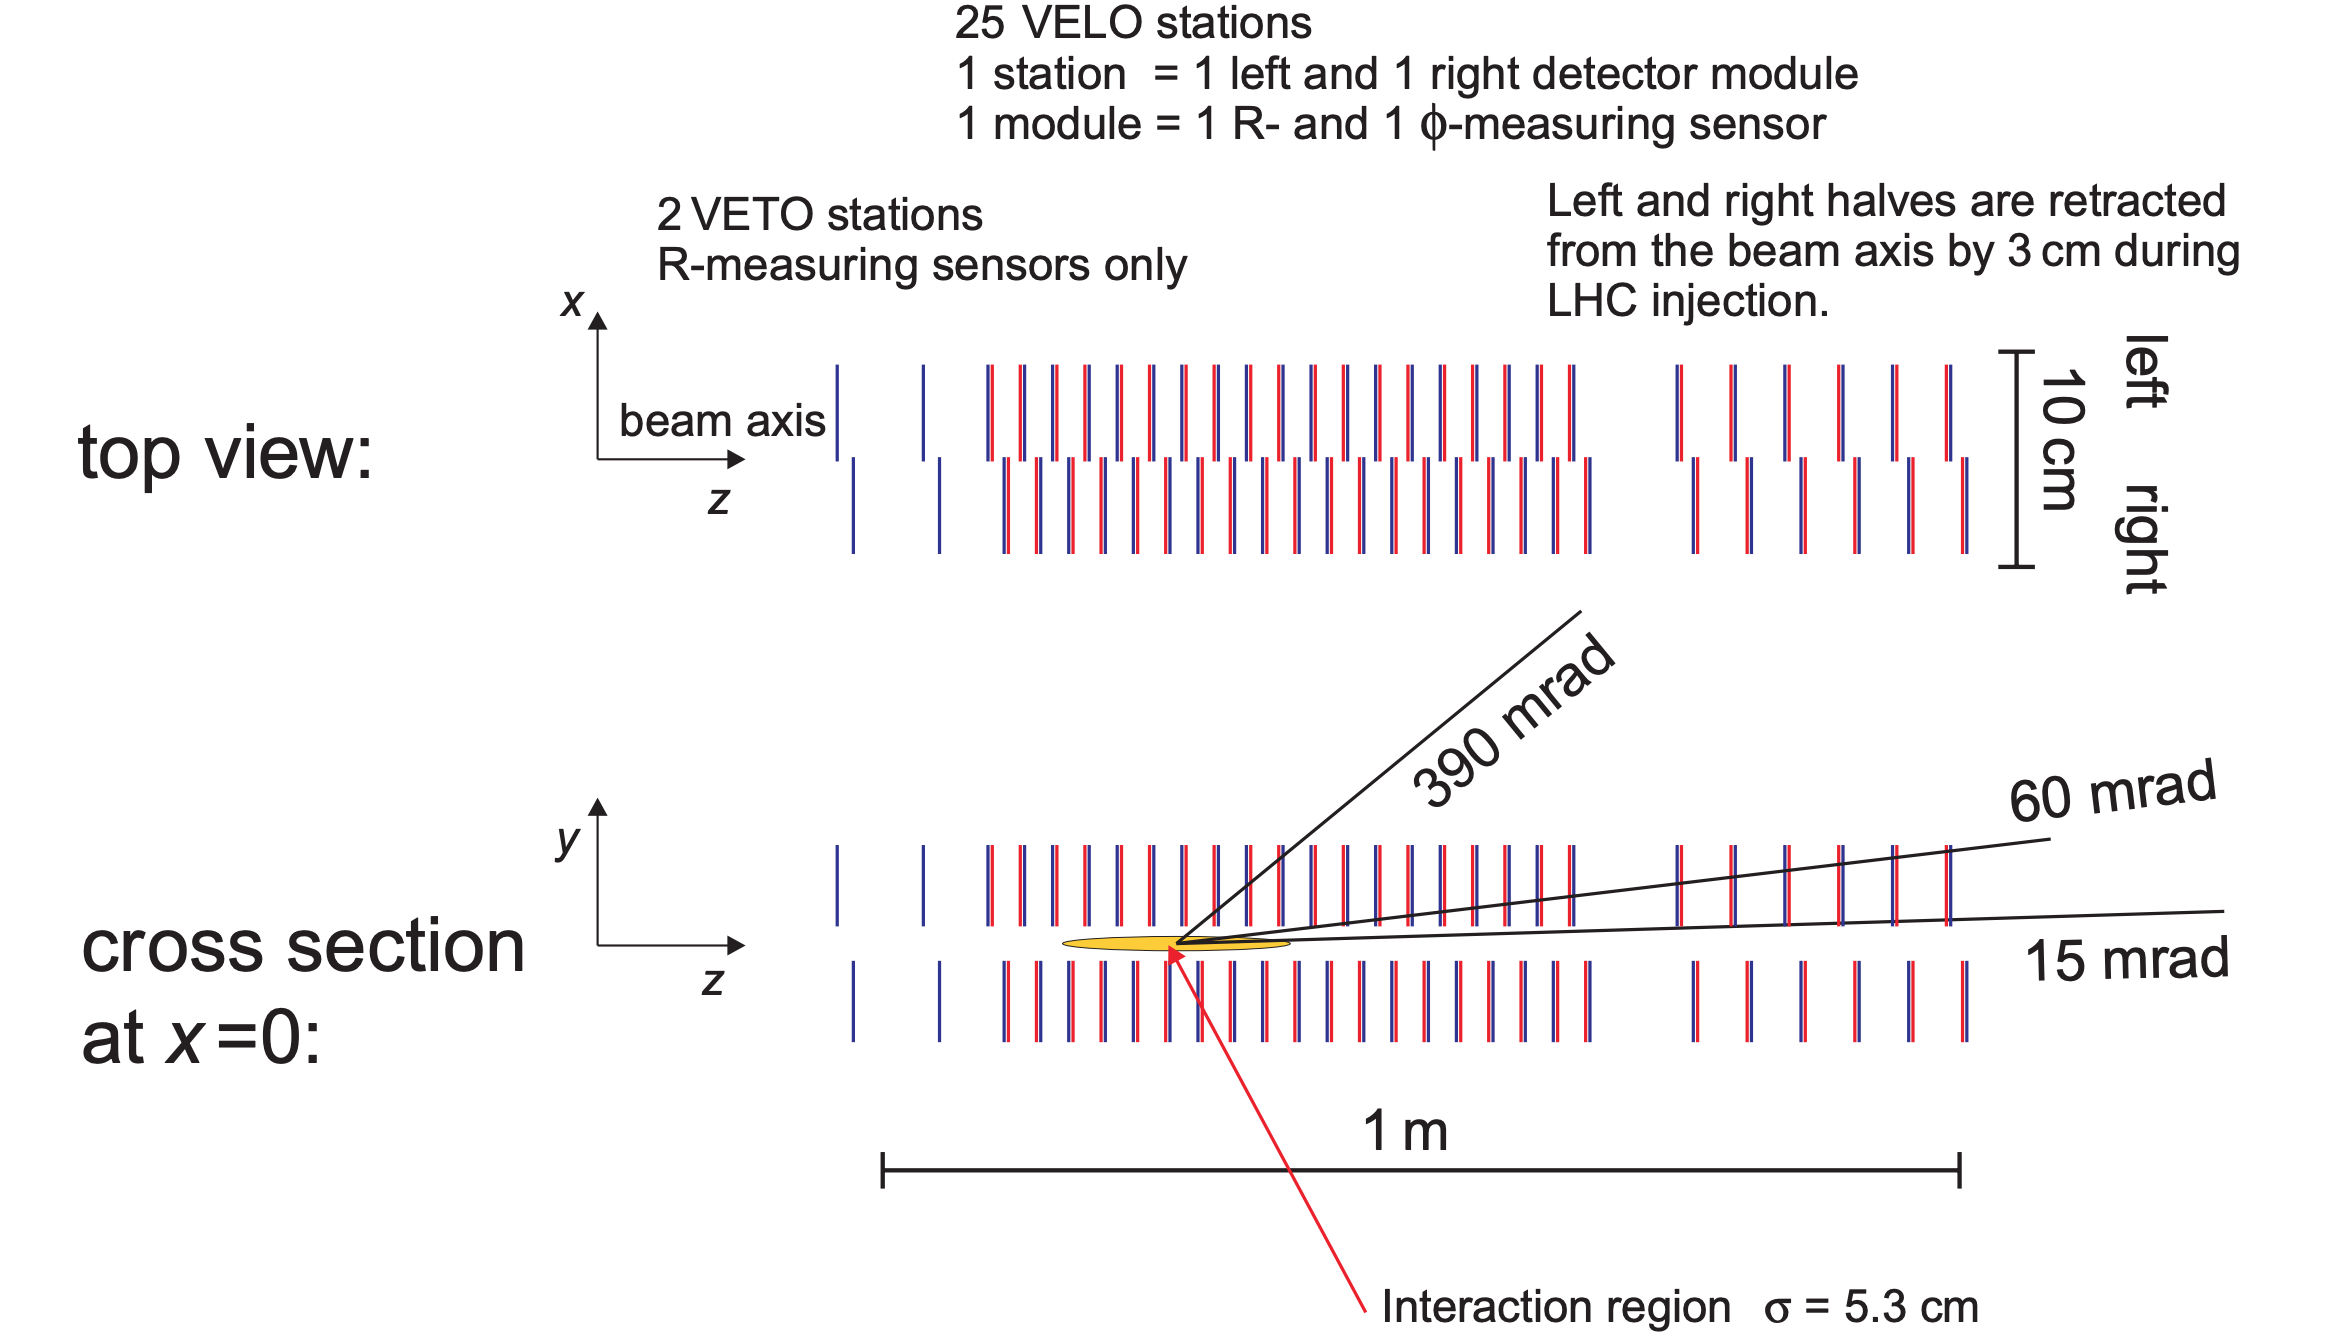
\includegraphics[width=0.95\columnwidth]{figures/detector/VELO_stations.png}
    \caption{Overview of the arrangement of VELO stations from the VELO Technical Design Report (TDR)~\cite{VELO-TDR}. The actual detector includes 21 stations instead of 25, but the overall design is identical~\cite{VELO-Performance}.}
    \label{fig:VELO_stations}
\end{figure}

\begin{figure}[tb]
    \centering
    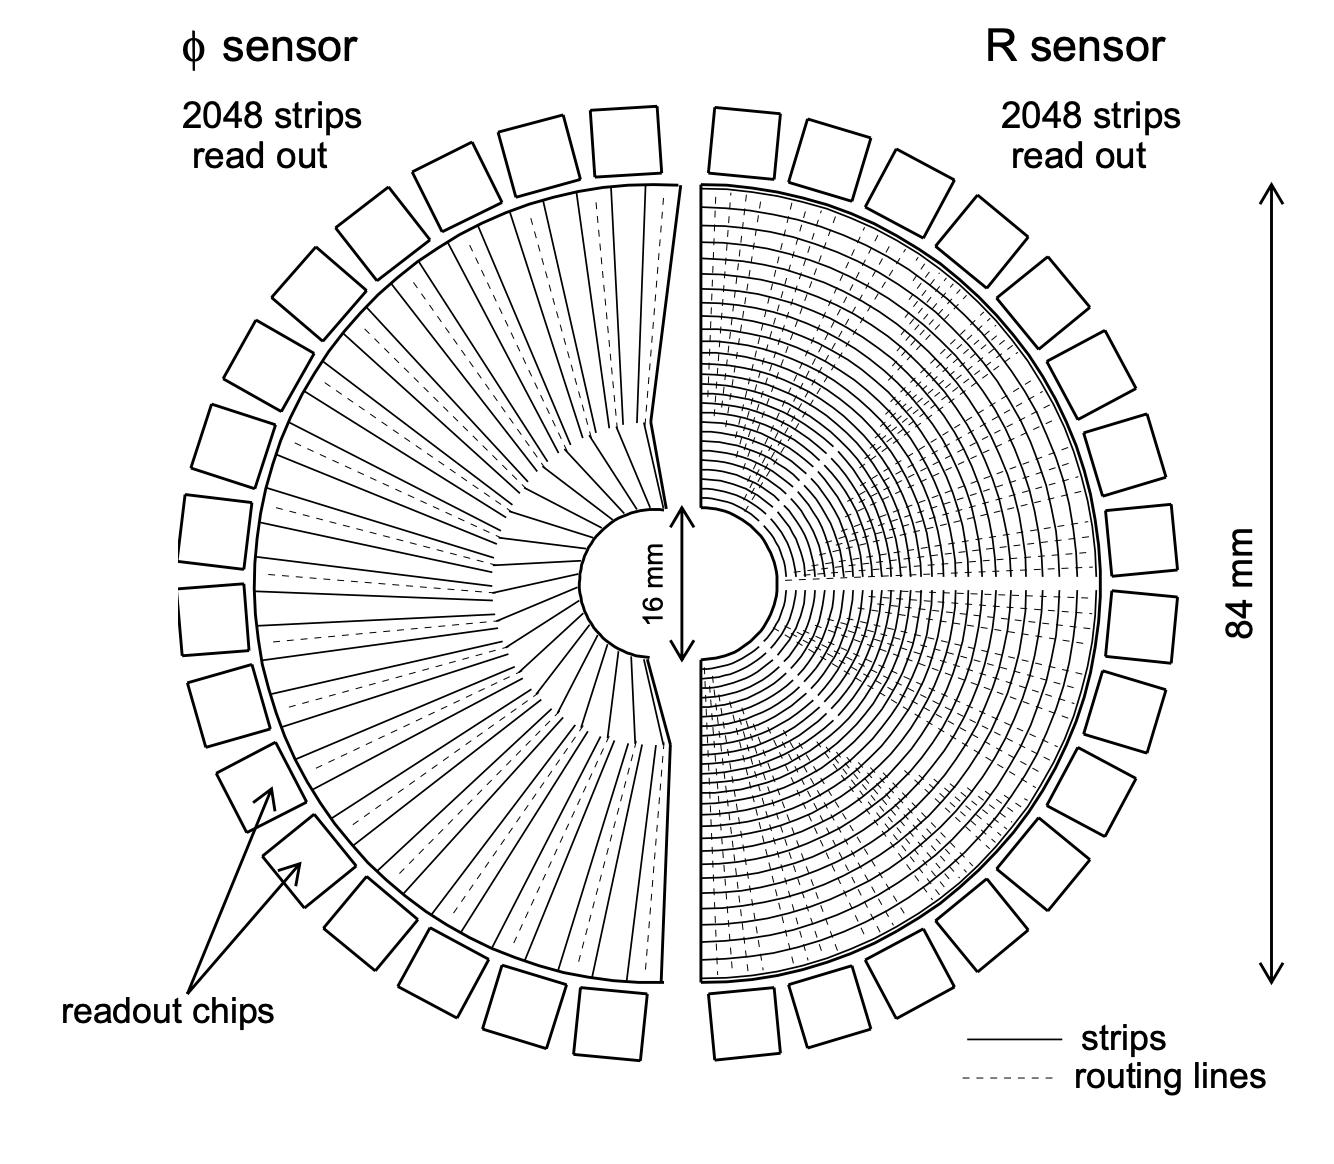
\includegraphics[width=0.55\columnwidth]{figures/detector/VELO_sensors.png}
    \caption{Illustration of the silicon strip layout in the VELO modules designed to measure (left) the azimuthal angle, $\phi$, of a track, and (right) the radial distance from the beam, $r$. Reproduced from Ref.~\cite{VELO-TDR}.}
    \label{fig:VELO_sensors}
\end{figure}

The primary vertex (PV) resolution of the VELO is typically $\sim $10\mum in the $x$ and $y$ directions and $\sim$50\mum in the $z$ direction, improving with the number of tracks originating at the PV, and deteriorating with the overall number of PVs~\cite{VELO-Performance}. The typical uncertainty on the decay length of a \B meson is about $230\mum$, compared to a typical decay length$~O(10)\mm$. The resolution of the \emph{impact parameter}, IP, of a track is well-described by the formula $\sigma_\mathrm{IP}=(15+29/[p_T/(\gev/c)])\mum$. This parameter excellently distinguished particles produced in secondary decays, from those produced in the primary interaction (for which the IP would be zero, were it not for the experimental resolution).
% subsection the_velo (end)

\subsection{Magnet and tracking stations} % (fold)
\label{sub:magnet_and_tracking_stations}

The \lhcb experiments uses a warm (non-superconducting) dipole magnet to measure the momentum of charged particles, by providing a maximum magnetic field strength of approximate $1\T$ and a total bending power of about $4\,$T\,m over the region where $z\in[2.5, 8]\m$. The magnetic field has been measured to a relative precision of about $4\times 10^{-4}$ and is uniform within a percent within the tracking volume. The profile of the magnetic field along the $z$-axis is shown in Fig.~\ref{fig:track_types} on page~\pageref{fig:track_types}, where the track types within \lhcb are defined. The magnet can provide a magnetic field in either vertical direction; over the span of a year of  data taking approximately equal amounts of data are collected with the magnet in the "Up" and "Down" configurations; this leads to a number of charge-asymmetry effects to cancel, significantly reducing potential systematic uncertainties. 

The tracking system consists of the VELO, and four other tracking stations: the Tracker Turicencis (TT) upstream of the magnet, and the tracking stations 1--3 (T1, T2, T3) downstream of the magnet. The downstream tracking stations each consist of an Inner Tracker (IT) based on silicon strips, and an Outer Tracker (OT) that employs drift tubes. 

\begin{figure}[tb]
    \centering
    \begin{subfigure}{0.55\columnwidth}
        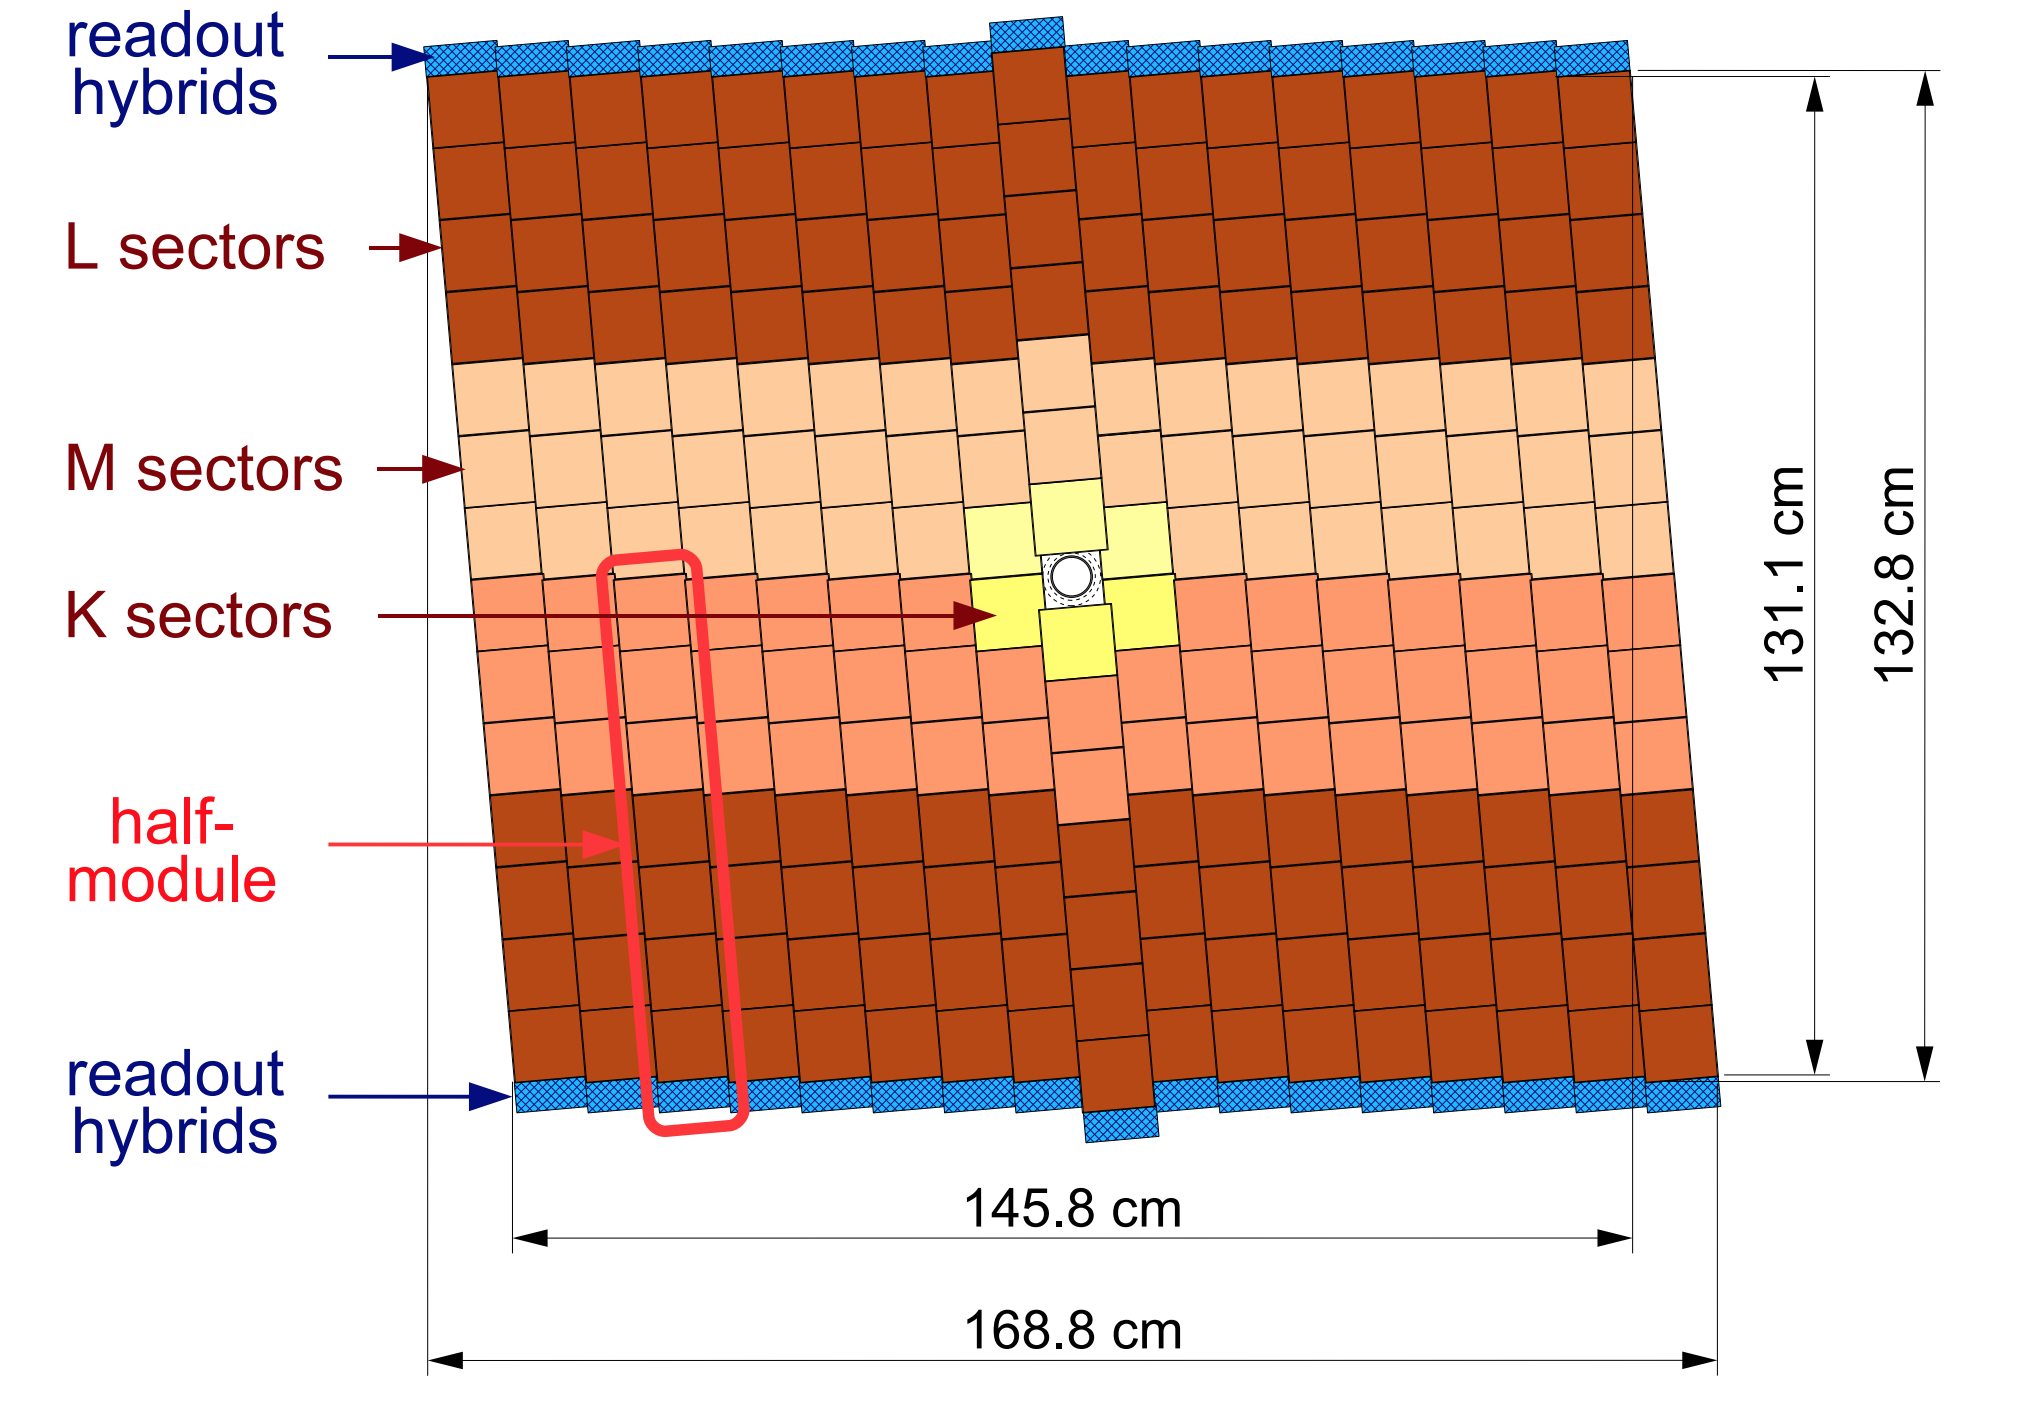
\includegraphics[width=\columnwidth]{figures/detector/TT_station.png}
        \caption{\label{fig:TT_station}}
    \end{subfigure}
    \begin{subfigure}{0.42\columnwidth}
        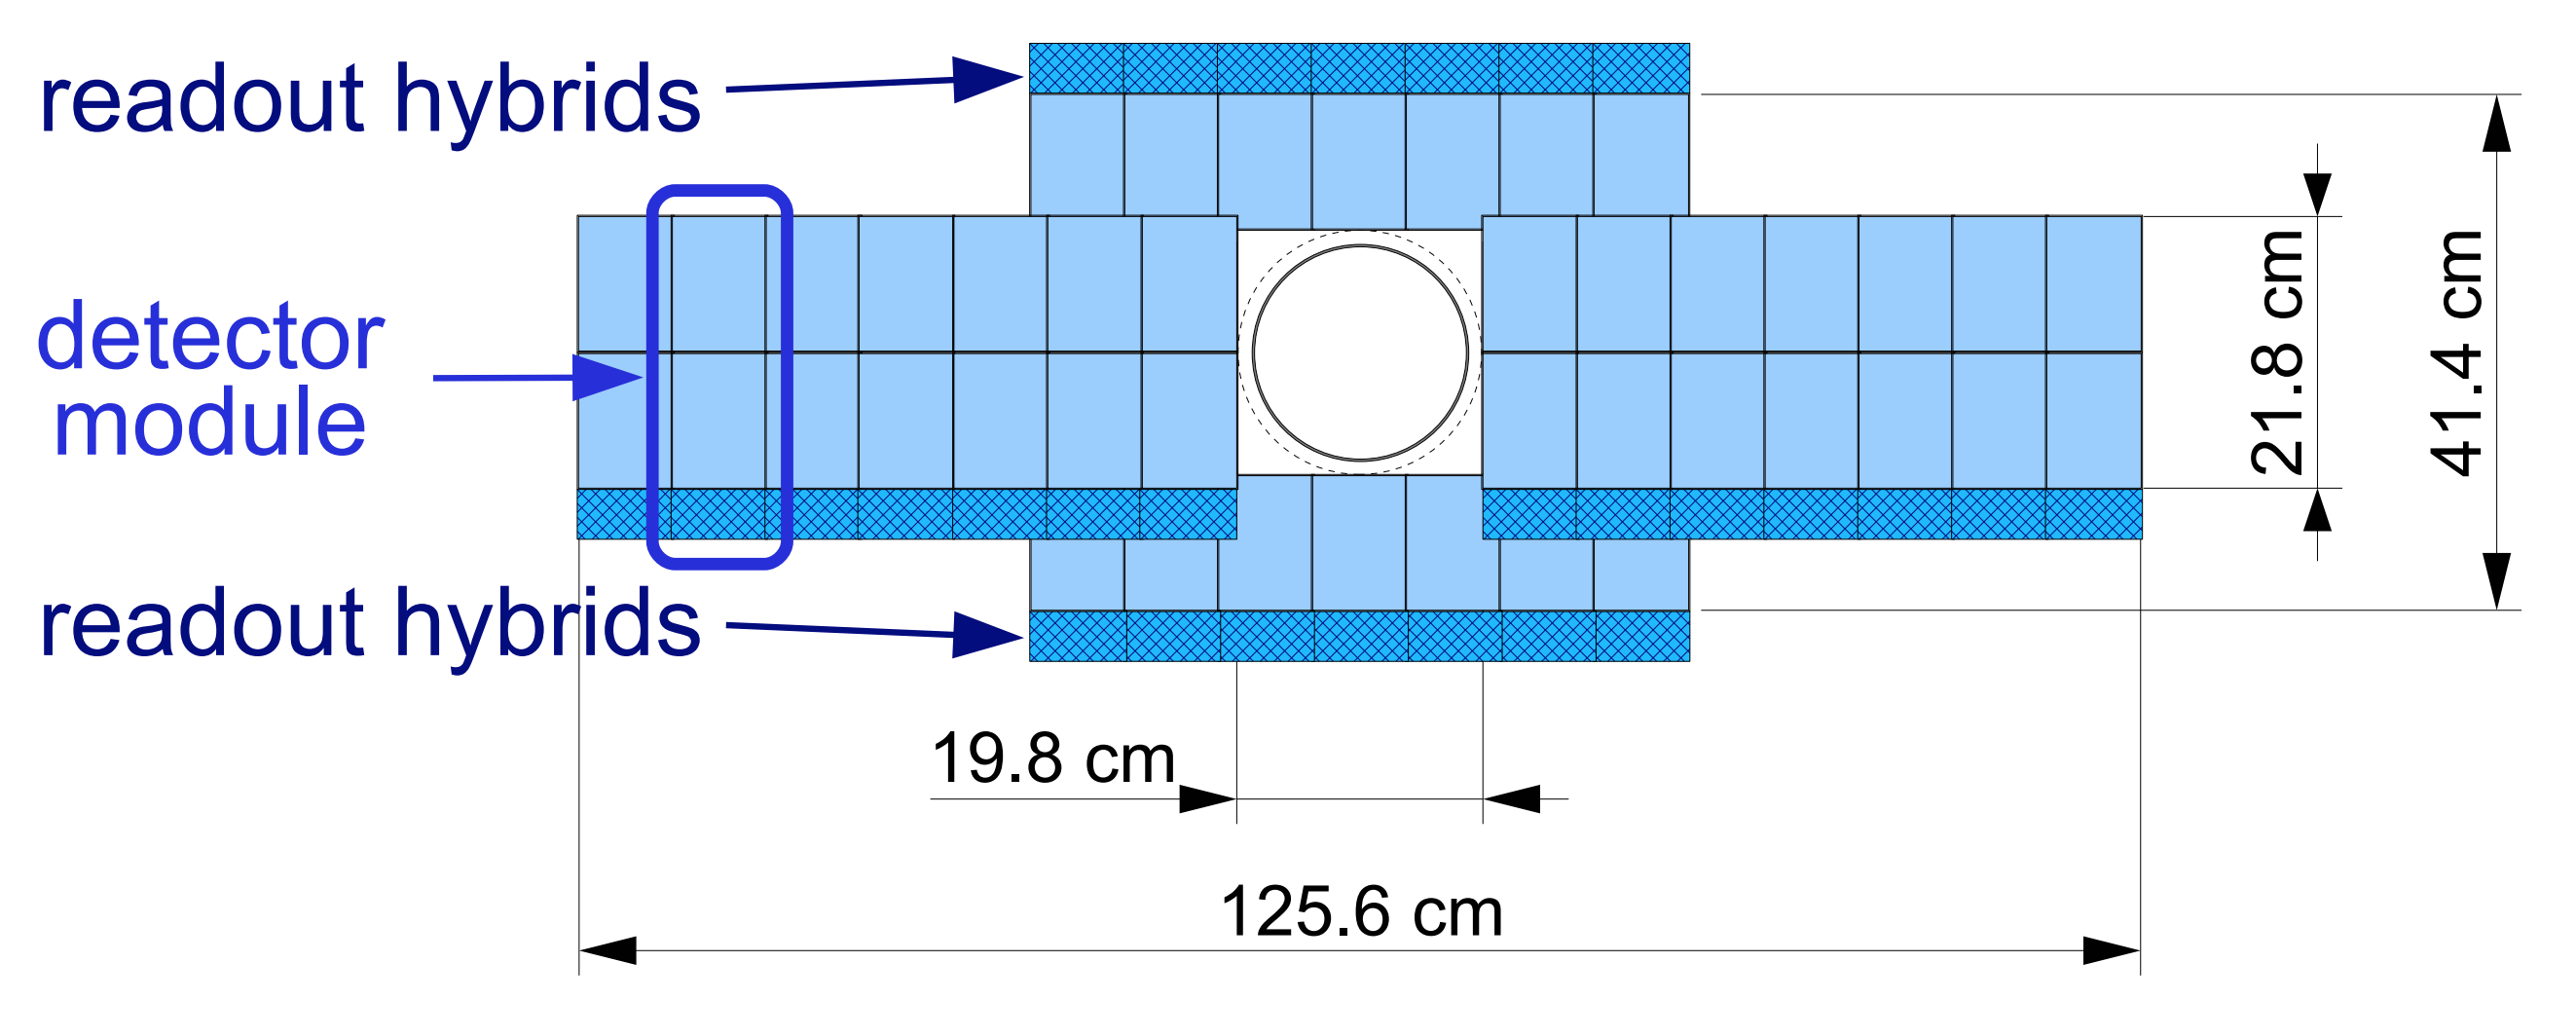
\includegraphics[width=\columnwidth]{figures/detector/IT_station.png}
        \caption{\label{fig:IT_station}}
    \end{subfigure}
    \caption{Overview of (a) a $v$-layer module of the IT and (b) and $x$-layer module of the IT. Reproduced from Ref.~\cite{LHCb-detector}}
    \label{fig:TT_IT_stations}
\end{figure}

Both the TT and IT are based on silicon strip detectors with a pitch of about $200\mum$; they were developed as a single project and are collectively known as the Silicon Tracker (ST). The TT  is a 140\cm wide and 130\cm tall planar tracking station, covering the whole \lhcb acceptance. It is shown in Fig.~\ref{fig:TT_station}. At each of the T1--T3 stations,  the IT consist of four modules, arranged around the beam pipe as illustrated in Fig.~\ref{fig:IT_station}. They do now cover the full \lhcb acceptance, only the very-forward region where the number of tracks is largest. Each TT or IT module comprises of four layers of silicon strips, where the central two layers are rotated $\pm5^\circ$ with respect to the first and last layer (an $x$-$u$-$v$-$x$ geometry). The ST has a spatial resolution for a given track of approximately 50\mum, chosen because the overall momentum resolution is then dominated by multiple-scattering effects for almost all momenta.

\begin{figure}[tb]
    \centering
    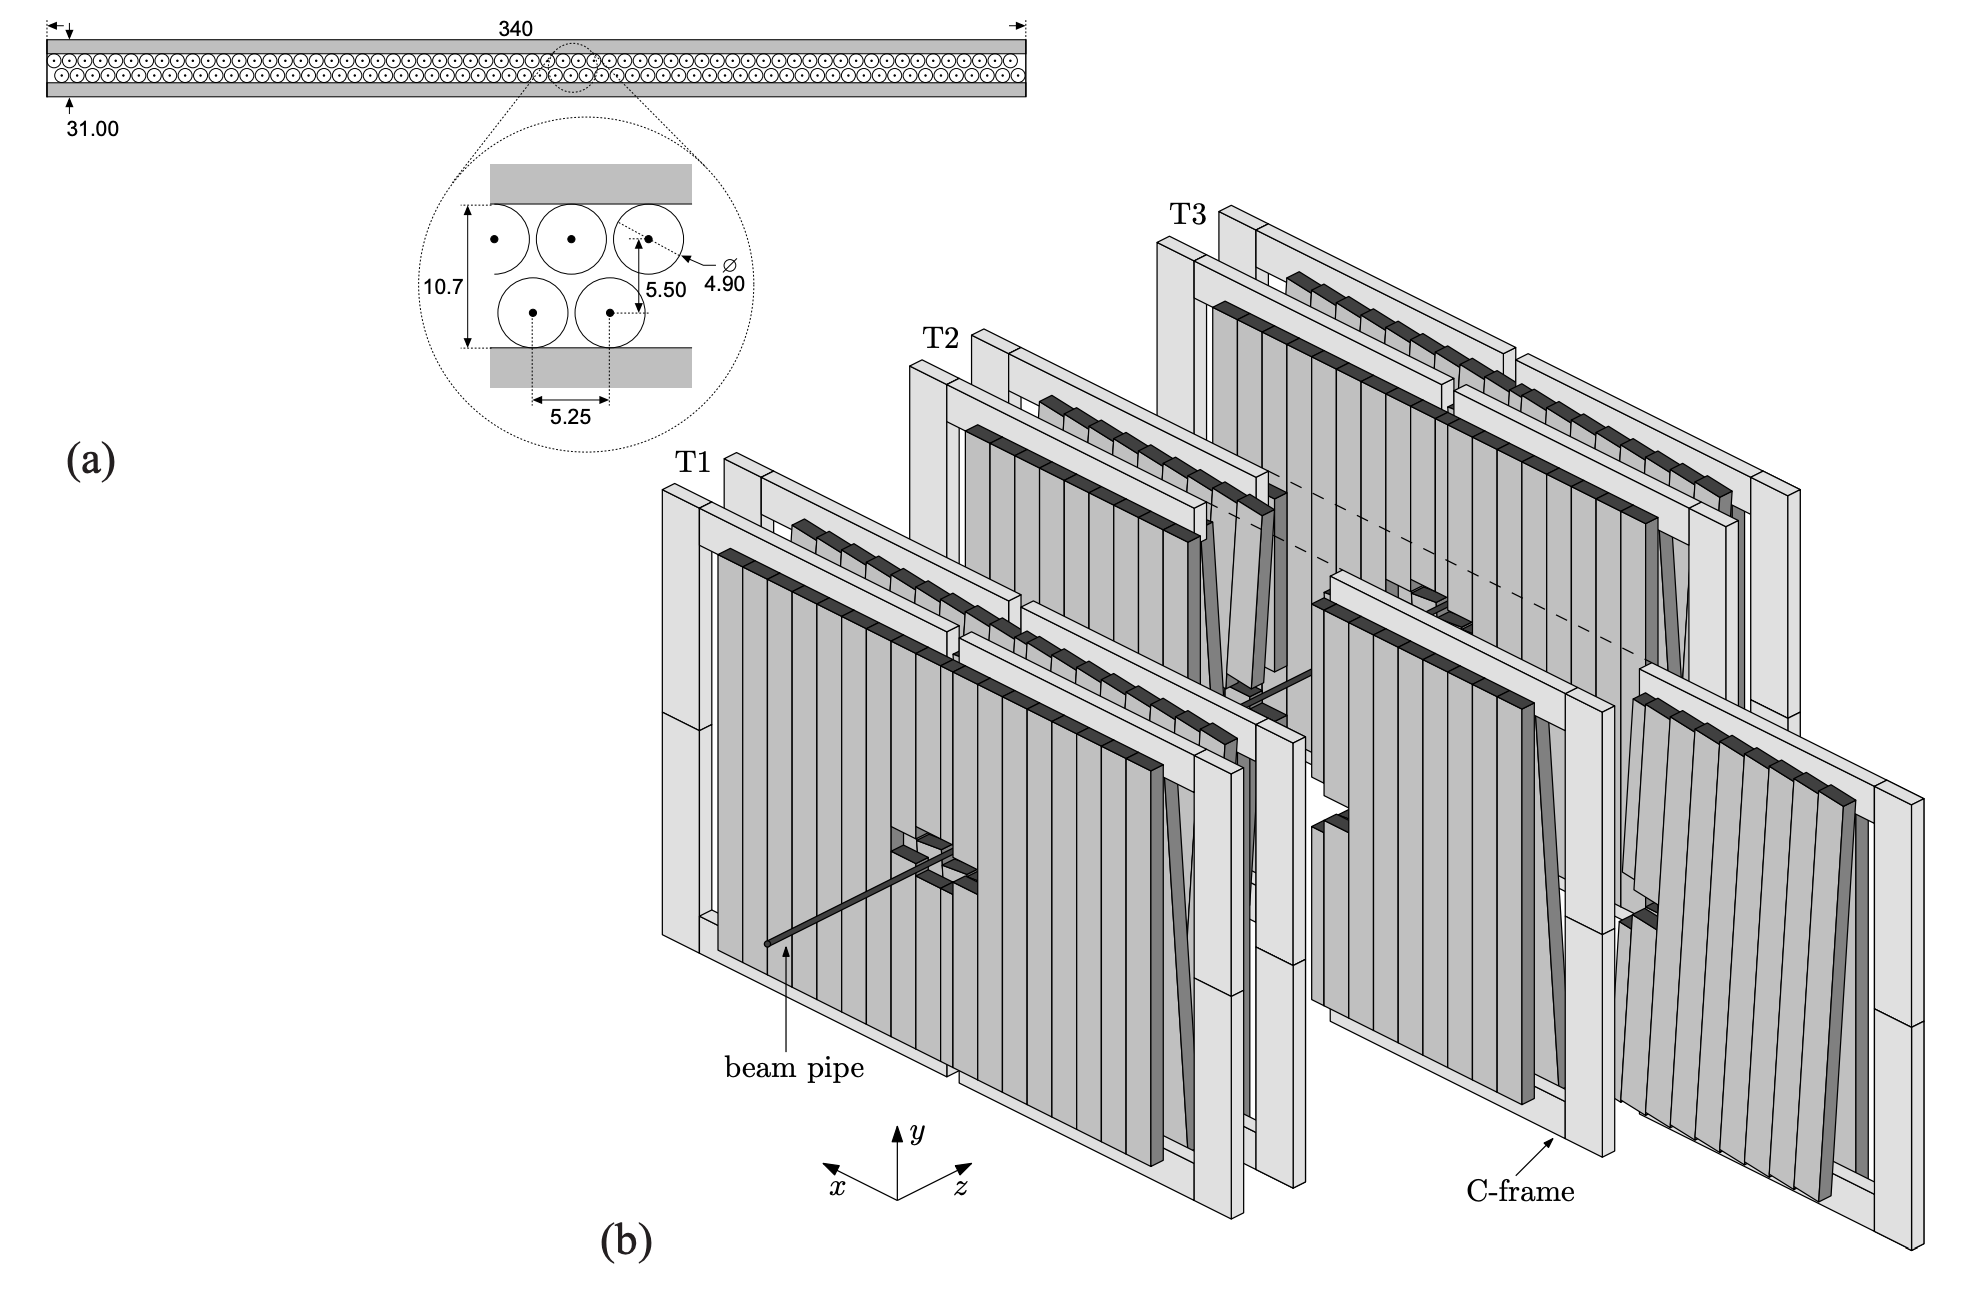
\includegraphics[width=\columnwidth]{figures/detector/OT_stations.png}
    \caption{(a) Cross section of an OT module. (b) Arrangement of the OT modules in tracking stations. Reproduced from Ref.~\cite{OT-Performance}.}
    \label{fig:OT_station}
\end{figure}

At the T1--T3 stations, the OT covers the part of the overall acceptance of 300 (250)\,mrad in the horizontal bending (vertical non-bending) plane that is not covered by the IT. The OT consists of arrays of gas-tight drift tubes with inner diameters of 4.9\mm. The OT is shown illustrated in Fig.~\ref{fig:OT_station}. An Ar/CO$_2$/O$_2$ (70/28.5/1.5) gas mixture is used to fill the tubes that ensures a drift time below 50\ns and a drift coordinate resolution of 200\mum. The use of a drift-chamber detector is necessary, because it was not economically feasible to instrument the whole \lhcb acceptance with silicon strip detectors in T1--T3. The condition that the OT occupancy should not be above 10\,\% in typical run conditions determined the boundary between the IT and the OT. 

\begin{figure}[tb]
    \centering
    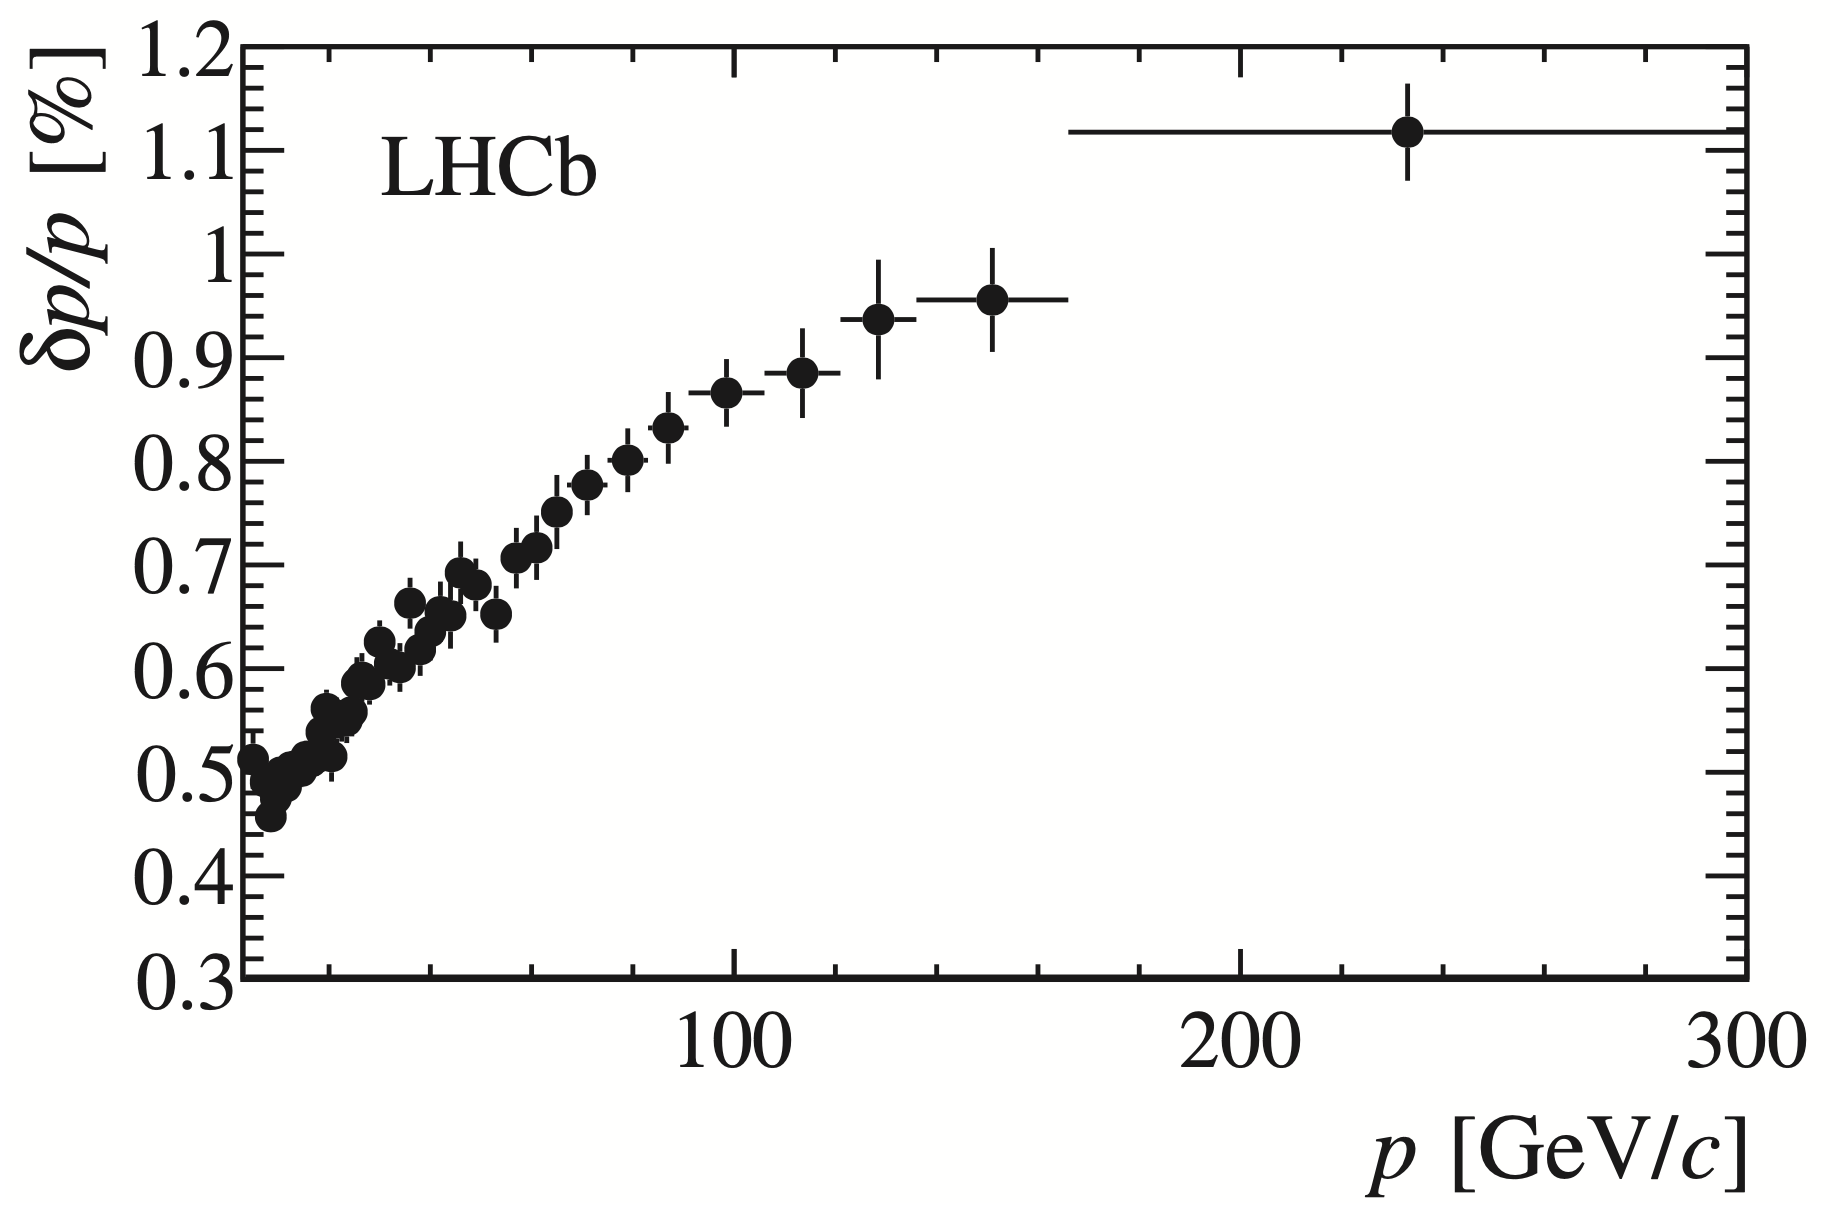
\includegraphics[width=0.55\columnwidth]{figures/detector/momentum_resolution.png}
    \caption{Relative uncertainty on the momentum of charged tracks (specifically long tracks, cf. the definitions in Section~\ref{sec:reconstruction}) in the \lhcb detector, determined via the mass resolution obtained in $J/\psi\to\mup\mu^-$ decays in Run~1 data. Reproduced from Ref.~\cite{LHCb-Performance}}
    \label{fig:momentum_resolution}
\end{figure}

The overall relative momentum resolution achieved for most charged tracks in \lhcb is less than a percent, as illustrated in Fig.~\ref{fig:momentum_resolution}, where it has been determined from a fit to the mass peak in $J/\psi\to\mup\mu^-$ decays in Run~1 data. 

% subsection magnet_and_tracking_stations (end) 

\subsection{The RICH detectors} % (fold)
\label{sub:the_rich}

\begin{figure}[tb]
    \centering
    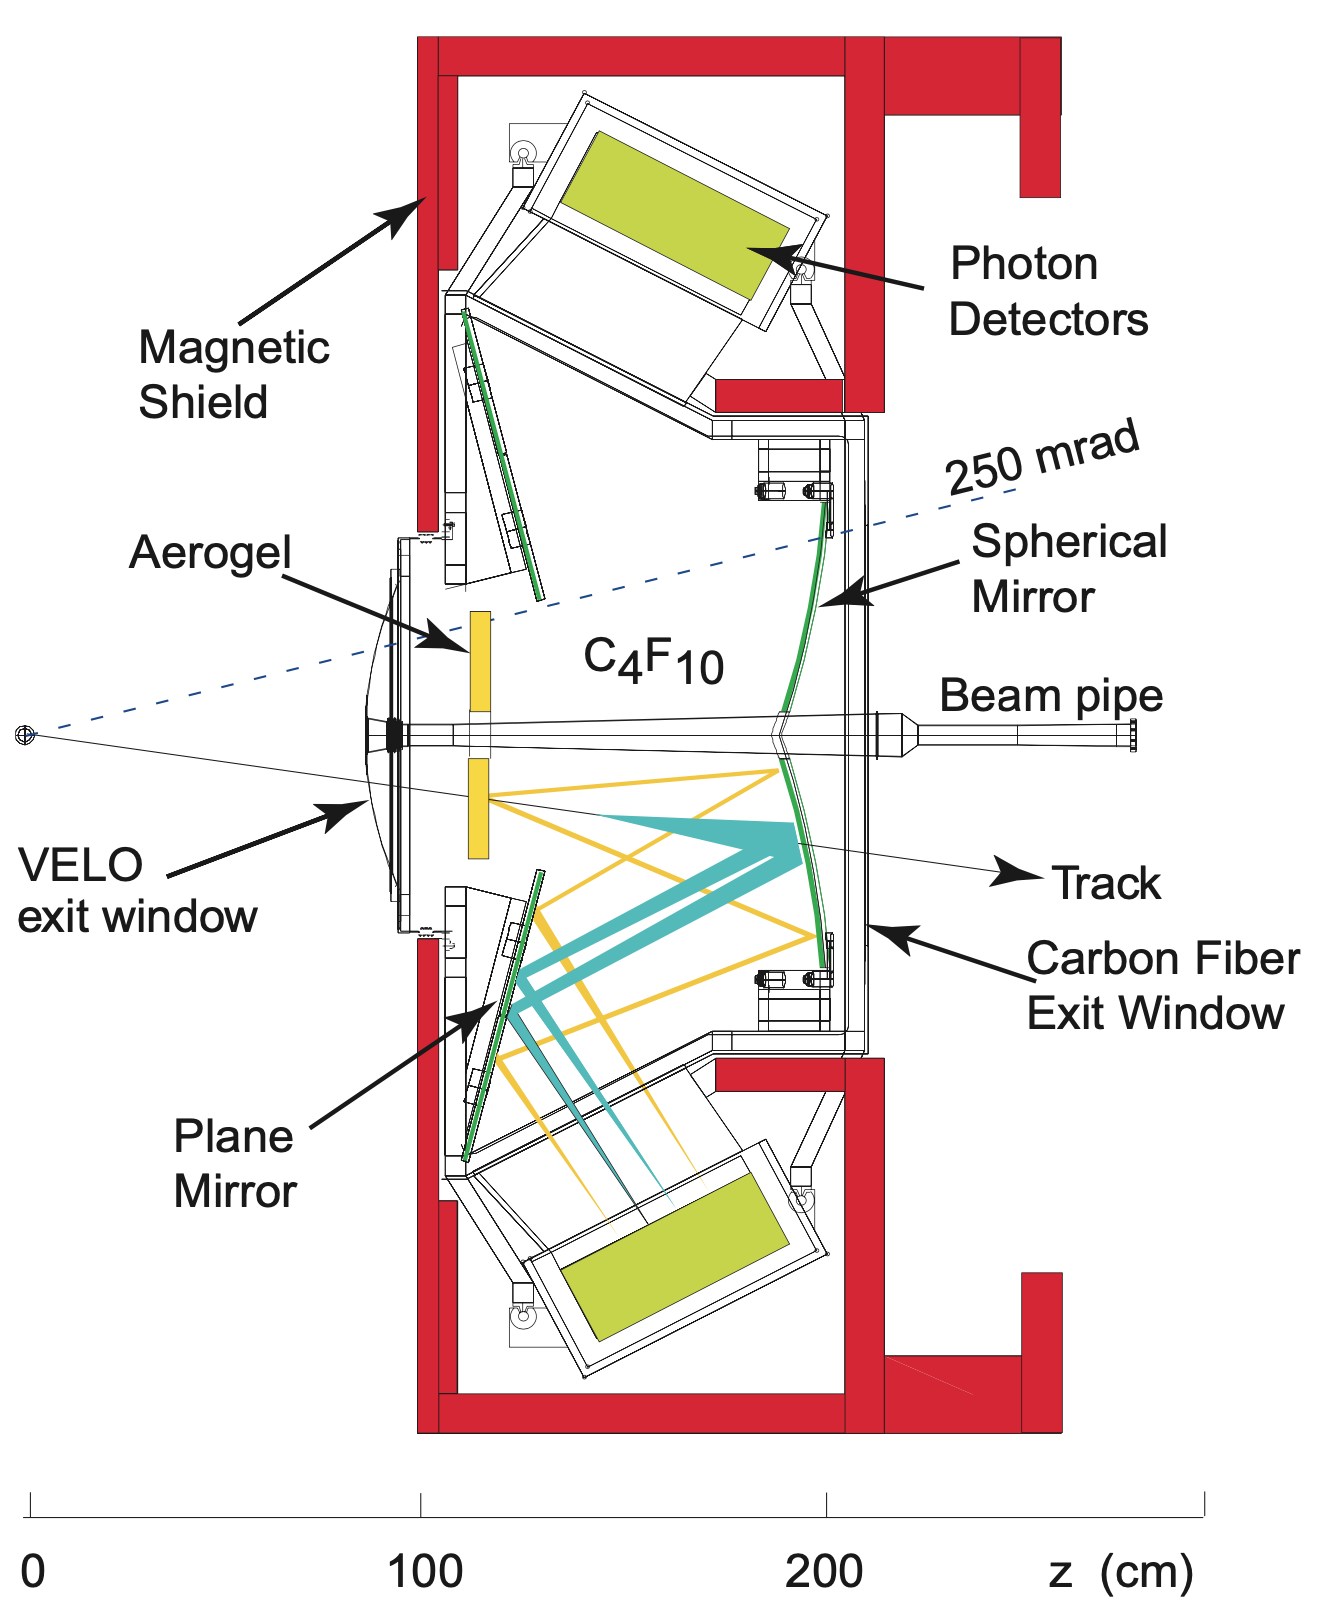
\includegraphics[width=0.45\columnwidth]{figures/detector/RICH1.png}
    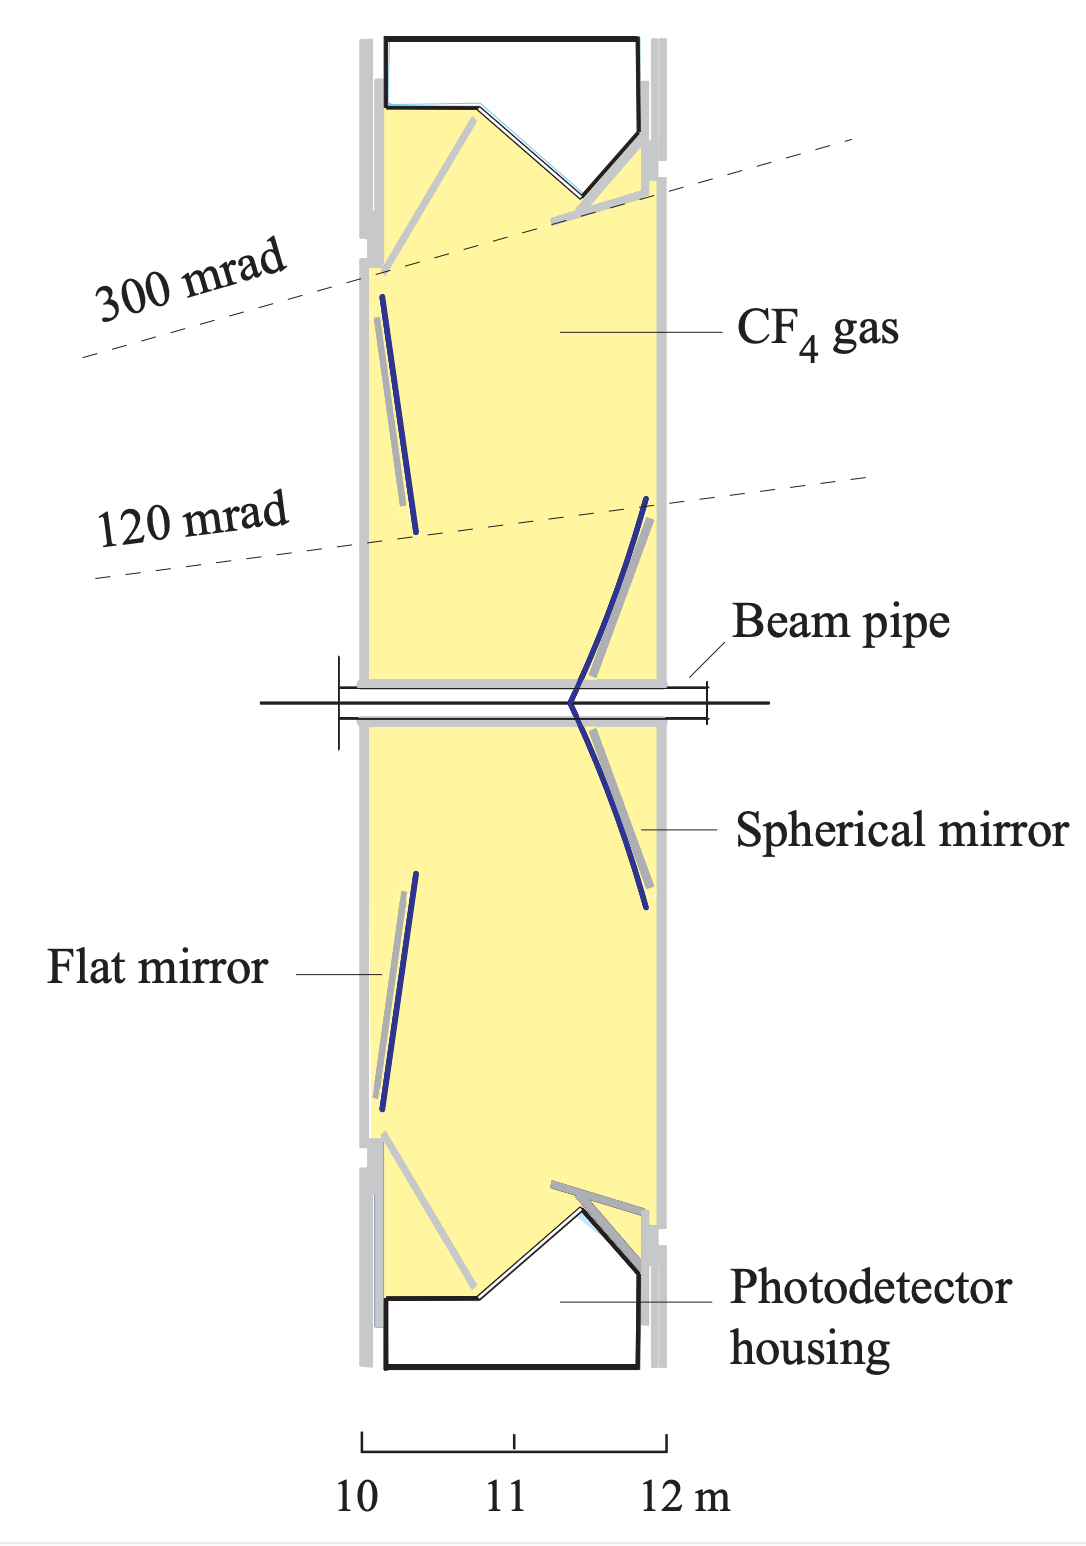
\includegraphics[width=0.4\columnwidth]{figures/detector/RICH2.png}
    \caption{Overview of (left) the Rich 1 and (right) the RICH 2 detectors. Reproduced from Ref.~\cite{LHCb-detector,RICH-TDR}.}
    \label{fig:RICHes}
\end{figure}

Two Ring Imaging CHerenkov detectors (RICH) provide crucial information for particle identification (PID) in \lhcb, in particular the ability to separate pions and kaons that is absolutely essential for the measurement presented in the thesis. The RICH 1 detector is located upstream of the magnet, in between the VELO and the TT tracking station. It is designed to provide PID capability for tracks in the momentum range $p\in[1-60]\gevc$ using a $\mathrm{C_4F_{10}}$ radiator, and covers the full \lhcb acceptance. During Run~1 the RICH 1 detector also included an Aerogel radiator designed to provide PID for very low momentum particles; however, it was removed before Run~2 because it did not meet the performance requirements during Run~1~\cite{RICH-Performance,RICH-Performance-2}. The RICH 2 detector is located downstream of the T1--T3 tracking stations. It is designed to provide PID capabilities for higher momentum tracks in the range $p\in[15-100]\gevc$ using a $\mathrm{CF_4}$ radiator. It only covers the very forward region where $|\theta| < 120$\,\mrad ($100$\,mrad) in the horizontal (vertical) directions, as high momentum particles are produced in that region. In both RICH detectors, mirrors are used to reflect the Cherenkov photons to arrays of Hybrid Photon Detectors (HPDs) located outside the \lhcb acceptance. The optics are designed such that photons originating from a given track form rings in the HPD arrays, where the radius is determined by the Cherenkov angle $\theta_c$. The detectors are illustrated in Fig.~\ref{fig:RICHes}.

\begin{figure}[tb]
    \centering
    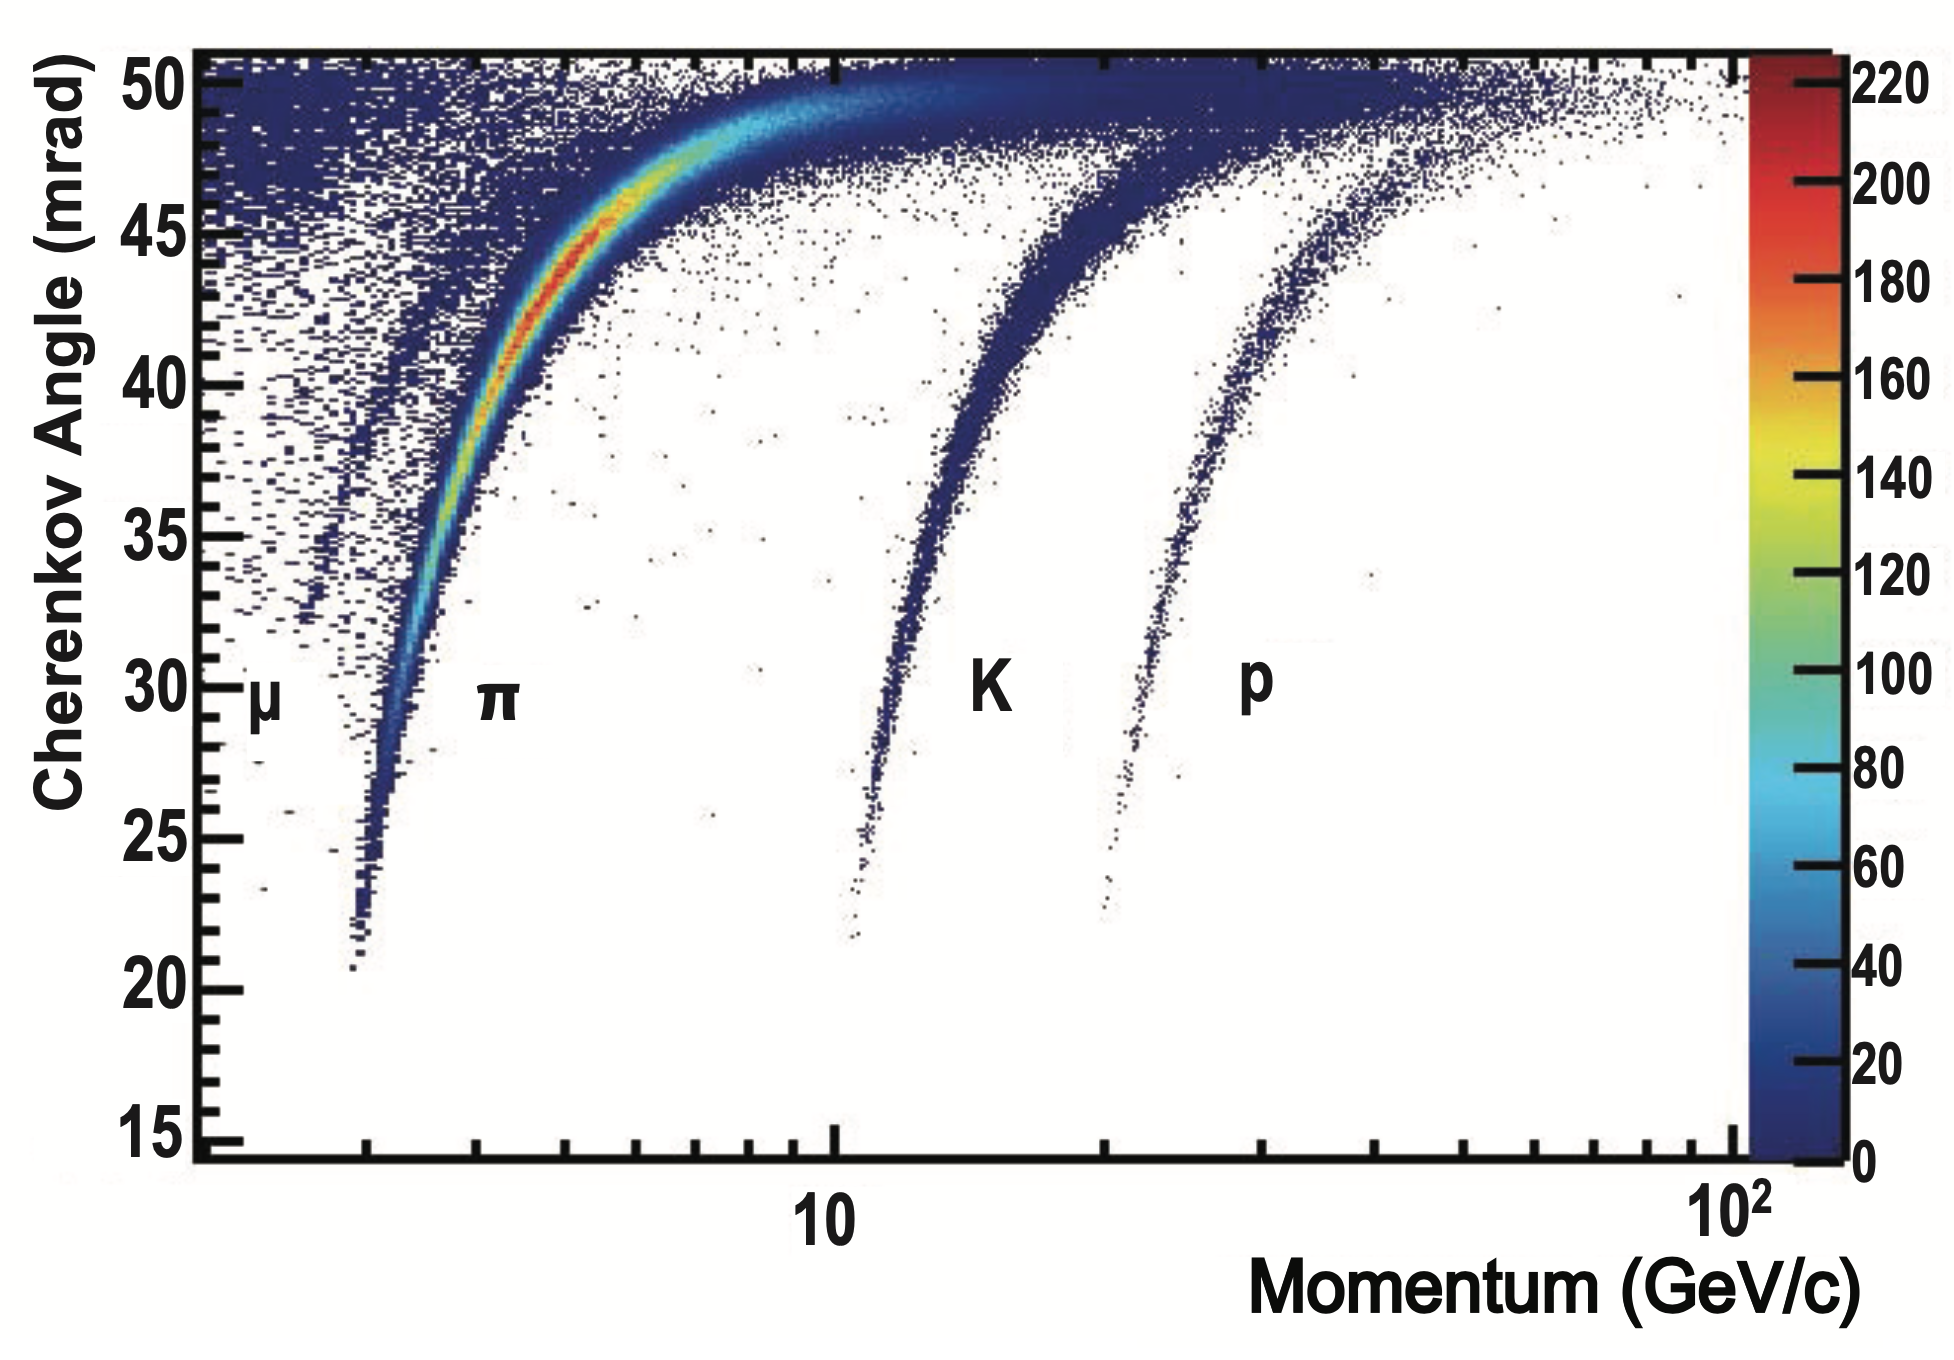
\includegraphics[width=0.55\columnwidth]{figures/detector/RICH_single_track.png}
    \caption{Cherenkov angle for isolated tracks in the RICH 1 radiator as a function of track momentum. Reproduced from Ref.~\cite{RICH-Performance}.}
    \label{fig:RICH_tracks}
\end{figure}

The resolution on $\theta_c$ can be measured by fitting the obtained $\theta_c$ distribution in high momentum tracks, where the Cherenkov angle is saturated. It is found to be $1.618 \pm 0.002$\,mrad for RICH 1 and $0.68 \pm 0.02$\,mrad for RICH 2 in Run~1 data~\cite{RICH-Performance}, and was essentially unchanged in Run~2~\cite{RICH-Performance-2}. Figure~\ref{fig:RICH_tracks} shows the relation between track momentum and $\theta_c$ in RICH 1 for \emph{isolated tracks} in Run~1 data; these are tracks where the Cherenkov ring does not overlap with any other Cherenkov rings. The bands for each hadron species are clearly visible, and it can be seen that the RICH detector also provide some ability to distinguish muons. The definition of the PID variables used in analysis is discussed in Section~\ref{sub:particle_identification}, along with the achieved PID performance.
% subsection the_rich (end)

\subsection{Calorimeters} % (fold)
\label{sub:calorimeters}

The calorimeter system of the \lhcb detector has four components. Ordered from the interaction point, these are the Scintillating Pad Detector (SPD), Pre-Shower (PS), an Electromagnetic CALorimeter (ECAL), and a Hadron CALorimeter (HCAL). Information from the calorimeters also provide identification of electrons, photons, and hadrons, and measurements of their energies and positions, and also plays a crucial role in the triggering, as described below. In all four cases, light is produced in organic scintillators and transmitted to Photo Multiplier Tubes (PMTs) via optical fibres~\cite{LHCb-detector}.

\begin{figure}[tb]
    \centering
    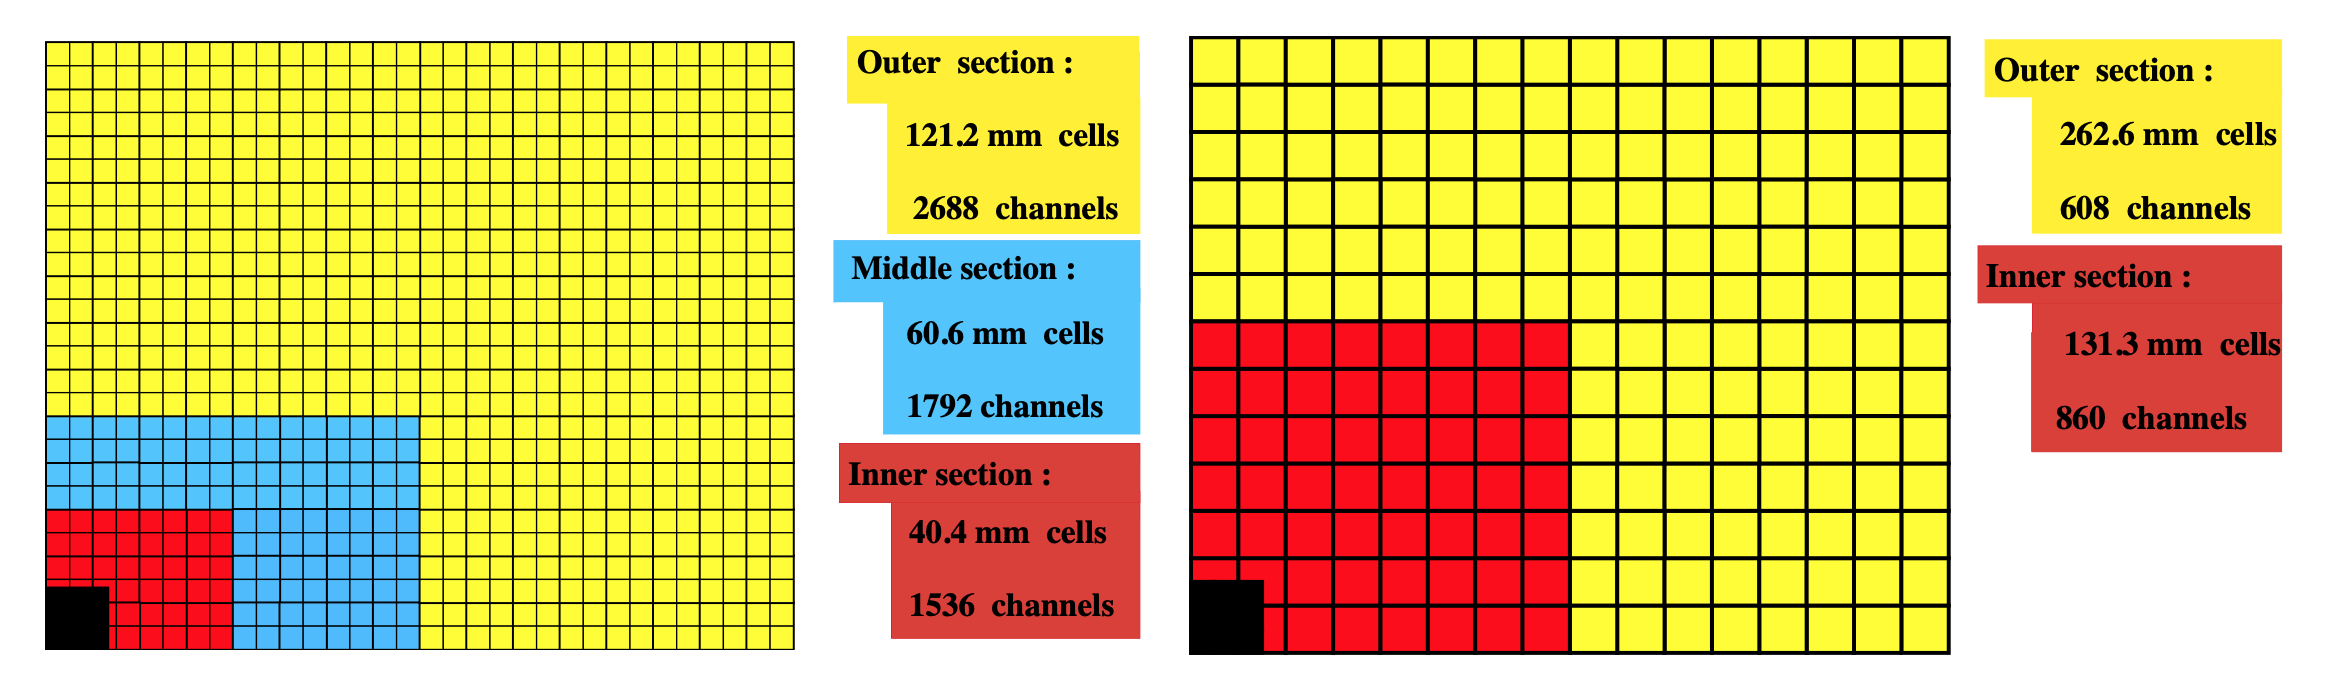
\includegraphics[width=0.9\columnwidth]{figures/detector/cell_modules.png}
    \caption{Illustration of the calorimeter cell size of (left) the ECAL and (right) the HCAL. Reproduced from Ref.~\cite{CAL-TDR}.}
    \label{fig:cal_cells}
\end{figure}

The SPD and PS detectors consist of almost identical planes of rectangular scintillator pads, with a 15\mm this lead absorber located in between. The presence of the SPD before the first absorption allows for the separation photons and charged particles using trigger information alone, because only electronic showers formed by the latter will deposit energy in the SPD. The PS allows for the separation of pion and electron tracks, as only the latter deposit significant energy in the thin lead layer. The cell divisions of the detectors closely follow that of the ECAL, shown in Fig.~\ref{fig:cal_cells}, to allow for the matching of energy deposits.

\begin{figure}[tb]
    \centering
    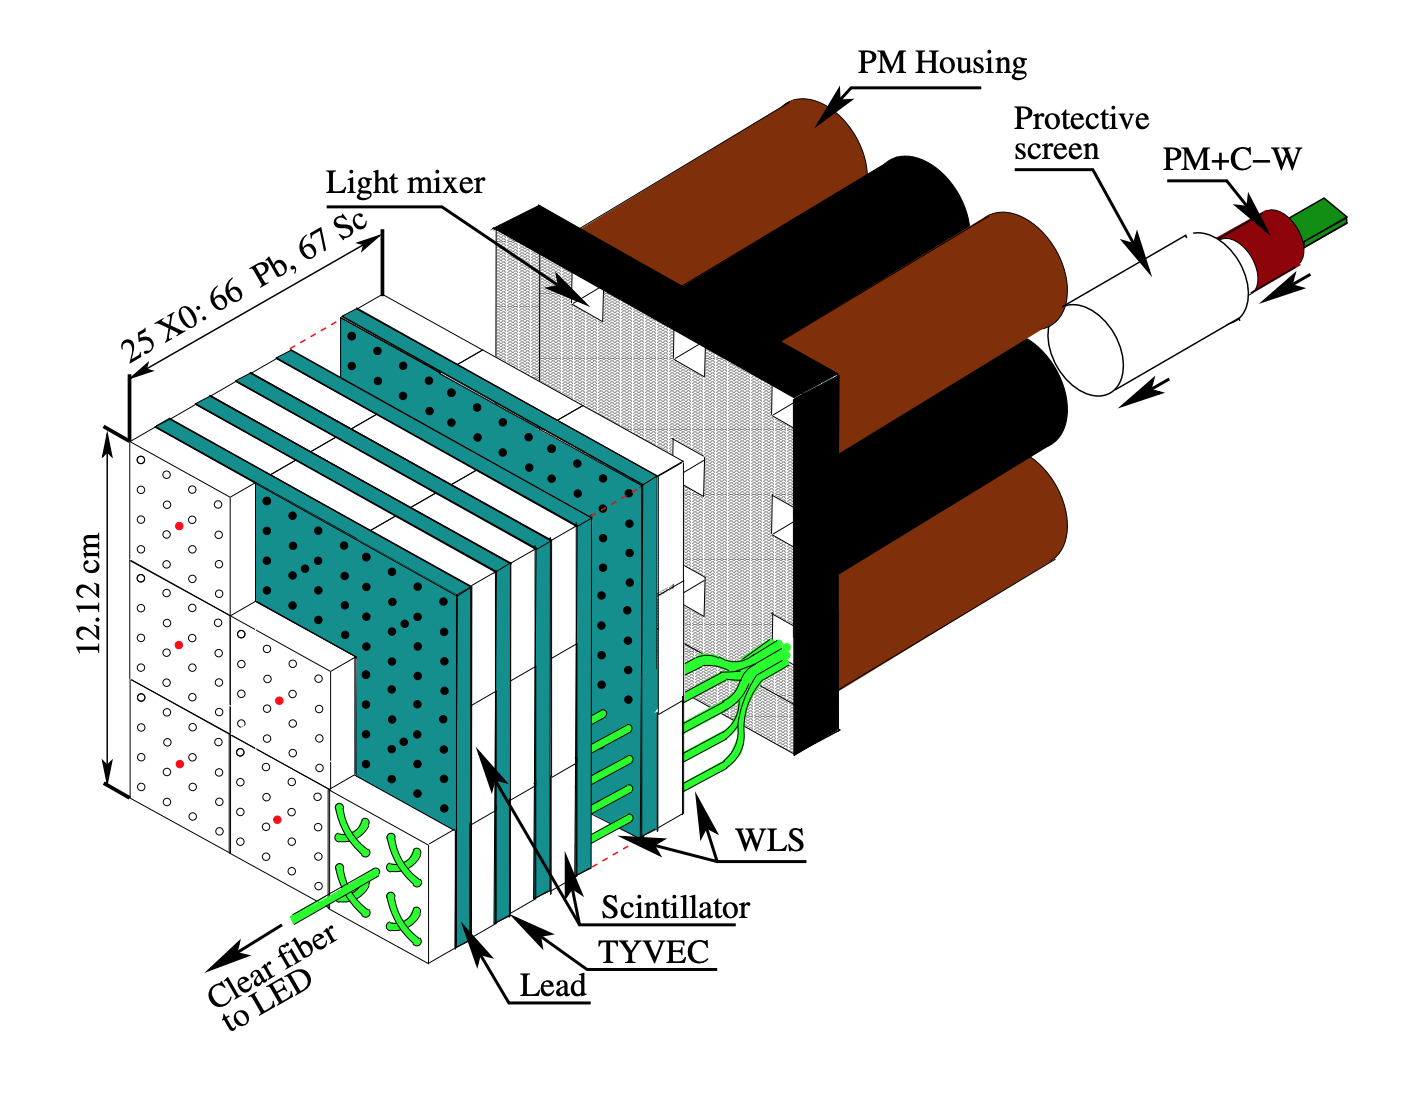
\includegraphics[width=0.55\columnwidth]{figures/detector/ECAL_module.png}
    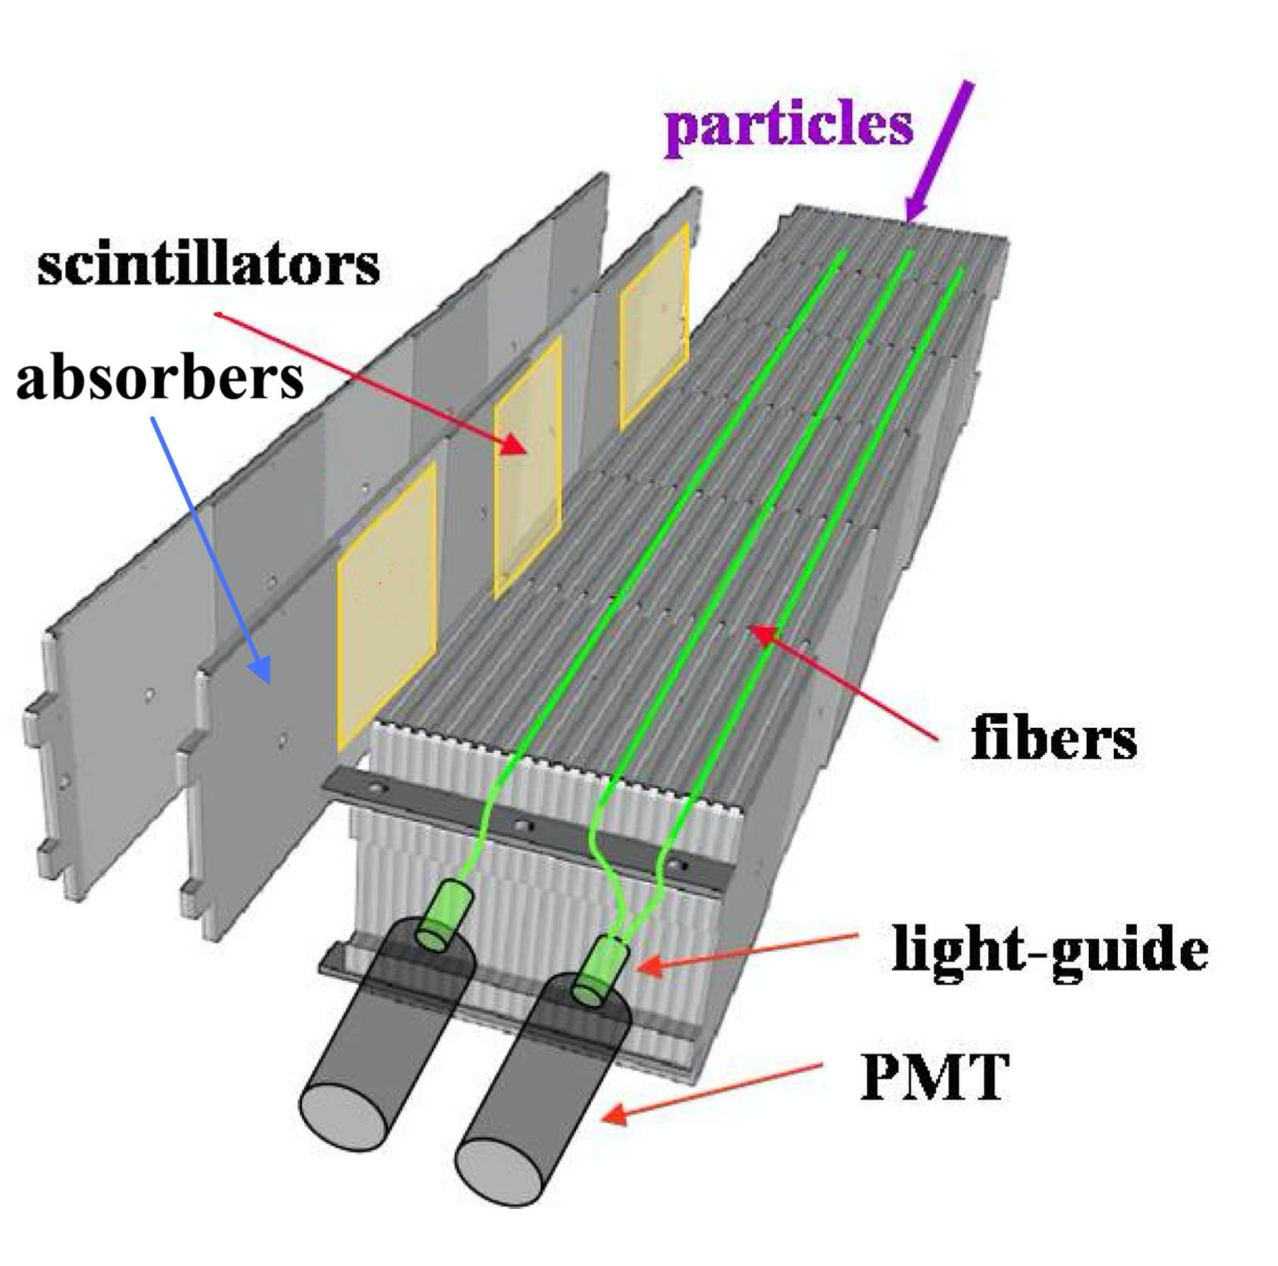
\includegraphics[width=0.40\columnwidth]{figures/detector/HCAL_module.png}
    \caption{Illustration of (left) an ECAL and (right) a HCAL module. Reproduced from Ref.~\cite{ECALpaper,LHCb-Performance}.}
    \label{fig:ECAL_HCAL_modules}
\end{figure}

The ECAL has a Shashlik structure, with 66 layers consisting of 2\mm of lead absorber and 4\mm of scintillator; an example of a calorimeter module is shown in Fig.~\ref{fig:ECAL_HCAL_modules}. Accurate energy measurements require that the full electronic shower is contained in the ECAL, which is achieved since the structure extends for 25 radiation lengths. The scintillators are divided into cells that allow for the determination of the location and shape of energy deposits; the cell dimensions vary as a function of radial distance from the beam pipe as shown in Fig.~\ref{fig:cal_cells}, to take into account the varying occupancy. The resolution of the ECAL has been measured to be $\Delta E/E \simeq (9/\sqrt{E} \bigoplus 0.8)\,\%$ ($E$ in \gevcc)~\cite{LHCb-detector}.

The HCAL is located downstream of the ECAL, designed to measure the energy of charged hadrons (which leave relatively little energy in the ECAL). It is constructed with layers of 1\cm iron absorbers inter-spaced with scintillators, oriented \emph{along} the beam direction, such that a typical track will traverse 16\mm of iron per 4\mm of scintillator~\cite{CAL-TDR}. As for the ECAL, the cell size varies as a function of distance to the beam line, as shown in Fig.~\ref{fig:cal_cells}. An example of a module is shown in Fig.~\ref{fig:ECAL_HCAL_modules}.  The energy resolution required for efficient triggering is moderate; therefore,  the HCAL only has a length of 5.6 interaction lenghts and can measure the hadron energies at a resolution of $\Delta E/E\simeq \simeq (69/\sqrt{E} \bigoplus 9)\,\%$ ($E$ in \gevcc)~\cite{LHCb-detector}.

% subsection calorimeters (end)

\subsection{Muon detectors} % (fold)
\label{sub:muon_detectors}

\begin{figure}[tb]
    \centering
\begin{subfigure}{0.45\columnwidth}
    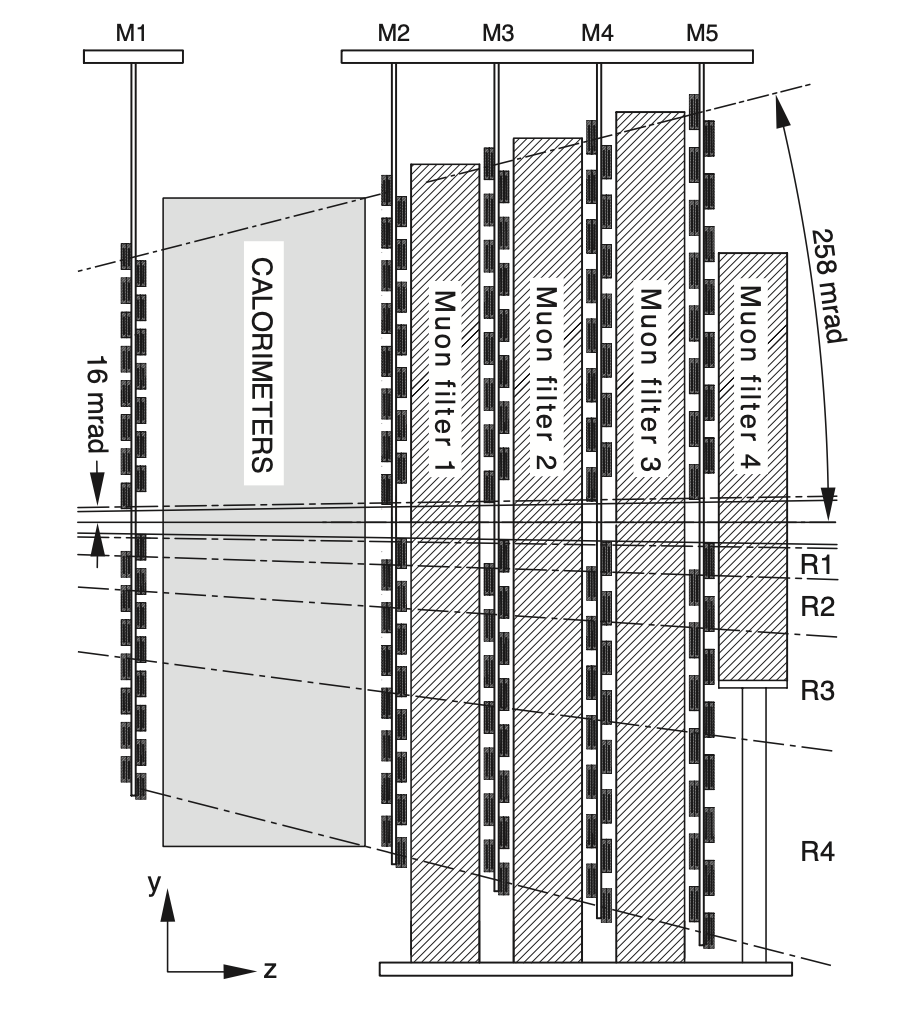
\includegraphics[width=\columnwidth]{figures/detector/muon_stations.png}
    \caption{}
    \label{fig:muon_stations}
\end{subfigure}
\begin{subfigure}{0.45\columnwidth}
    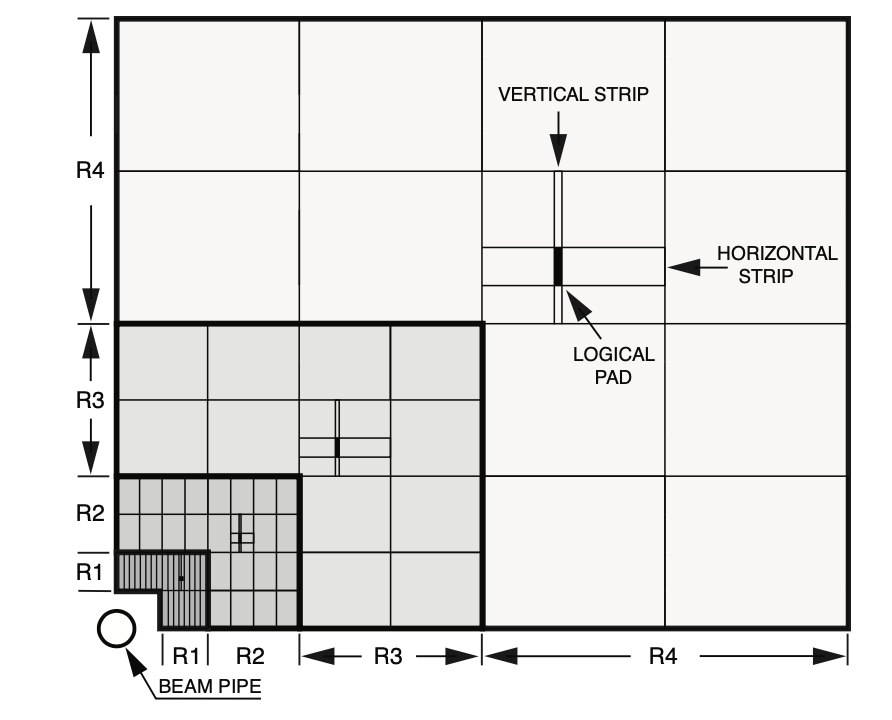
\includegraphics[width=\columnwidth]{figures/detector/muon_pad.png}
    \caption{}
    \label{fig:muon_pad}
\end{subfigure}
    \caption{Illustration of (a) the location of the muon stations along the $z$-axis of the experiment, and (b) the geometry of the logical pads of the M3 muon station. Reproduced from Ref.~\cite{LHCb-Performance}.}
\end{figure}

Muon identification and triggering is crucial for a range of high-profile \lhcb measurements, such as lepton-universality tests or measurements of  $B^0_{(s)}\to\mup \mu^-$ decays. In the thesis, muon identification plays a role in suppressing a number of backgrounds. The \lhcb muon system consists of 5 tracking stations, M1--M5, covering the full \lhcb acceptance. M1 is located upstream of the ECAL, whereas M2--M5 are located downstream of the HCAL and inter-spaced with 80\cm thick ion absorbers in order to select penetrating muons. This is illustrated in Fig.~\ref{fig:muon_stations}. The detectors are multiwire proportional chambers (MWPC), organised into logical pads, the dimensions of which define the $(x, y)$ resolution of the measured spatial points. As for the calorimeters, the size of the pads vary as a function of the radial distance from the beam pipe, as illustrated in Fig.~\ref{fig:muon_pad}. The resolution is significantly better in the bending plane ($x$) than in the non-bending plane ($y$). The resolution is also significantly better in the M1--3 stations than in M4 and M5, which are mostly used to identify penetrating tracks. The muon system can independently measure the $p_T$ of a muon to within 20\,\%, which allows for efficient triggering.

% subsection muon_detectors (end)

% section subdetectors (end)

\section{Reconstruction} % (fold)
\label{sec:reconstruction}

This section describes the reconstruction algorithms that fit the detector hits in the tracking stations to form track candidates, as well as the algorithms used to identify the types of the particles that formed these tracks.

% section reconstruction (end)

\subsection{Track reconstruction} % (fold)
\label{sub:track_reconstruction}

\begin{figure}[tb]
    \centering
    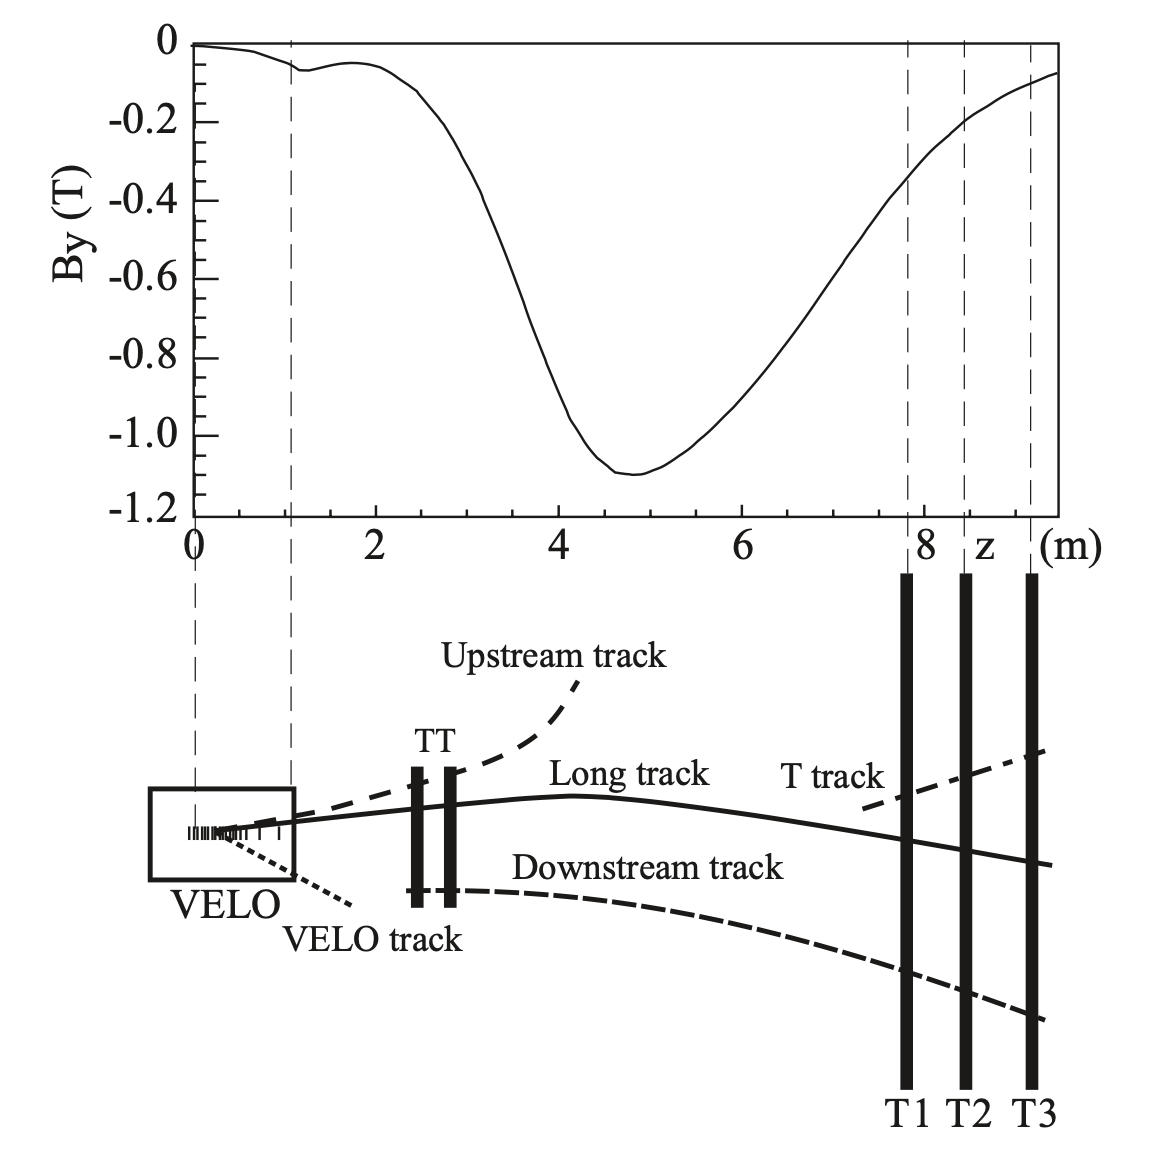
\includegraphics[width=0.75\columnwidth]{figures/detector/track_types.png}
    \caption{Definition of track types within the \lhcb detector, depending on which set of tracking detectors the track intersects. The profile of the magnetic field  is also shown. Reproduced from Ref.~\cite{LHCb-Performance}.}
    \label{fig:track_types}
\end{figure}

The \lhcb experiments operates with a number of different particle track types, depending on which sub detectors a track intersects; these are summarised in Fig.~\ref{fig:track_types}. The two track types that are important for this thesis are \emph{long} tracks, which have hits in the VELO and the TT and T1--T3 tracking stations, and \emph{downstream} tracks that only have hits in the TT and T1--3 tracking stations. The analysis depends on both track types because a number of \KS mesons produced in the signal decay leave the VELO before they decay into the $\pip\pim$ final state that is reconstructed; hence these pions necessarily form downstream tracks.

The first step is to form track candidates from hits in the VELO (VELO tracks) and T1--3 stations (T tracks) separately; because the magnetic field is low in the tracking detectors, these tracks are fairly straight. Long tracks are formed using two separate search strategies: in one, \emph{forward tracking}~\cite{VELO-Forward}, VELO tracks are used as seeds and matched with hits in the TT and T1--3 tracking stations by extrapolation. These are combined to form long tracks that are required to pass a set of quality conditions. An alternative approach, \emph{track matching}~\cite{VELO-Match,VELO-Match2}, matches VELO and T tracks by extrapolating both through the bending region, and deciding if they below together; finally TT hits are added. The union of tracks found via both approaches is saved, where only the track candidate with the best fit quality is kept in the case where a track appears twice. Downstream tracks are formed based on T tracks as seeds, matched with hits in the TT detector in a search region obtained by extrapolation of the seed~\cite{Downstream}. Finally, each track is reprocessed using a Kalman filter that takes into account multiple scattering and corrects for energy loss due to ionisation~\cite{fruhwirthApplicationKalmanFiltering1987,VanTilburg:885750}.

\begin{figure}[tb]
    \centering
    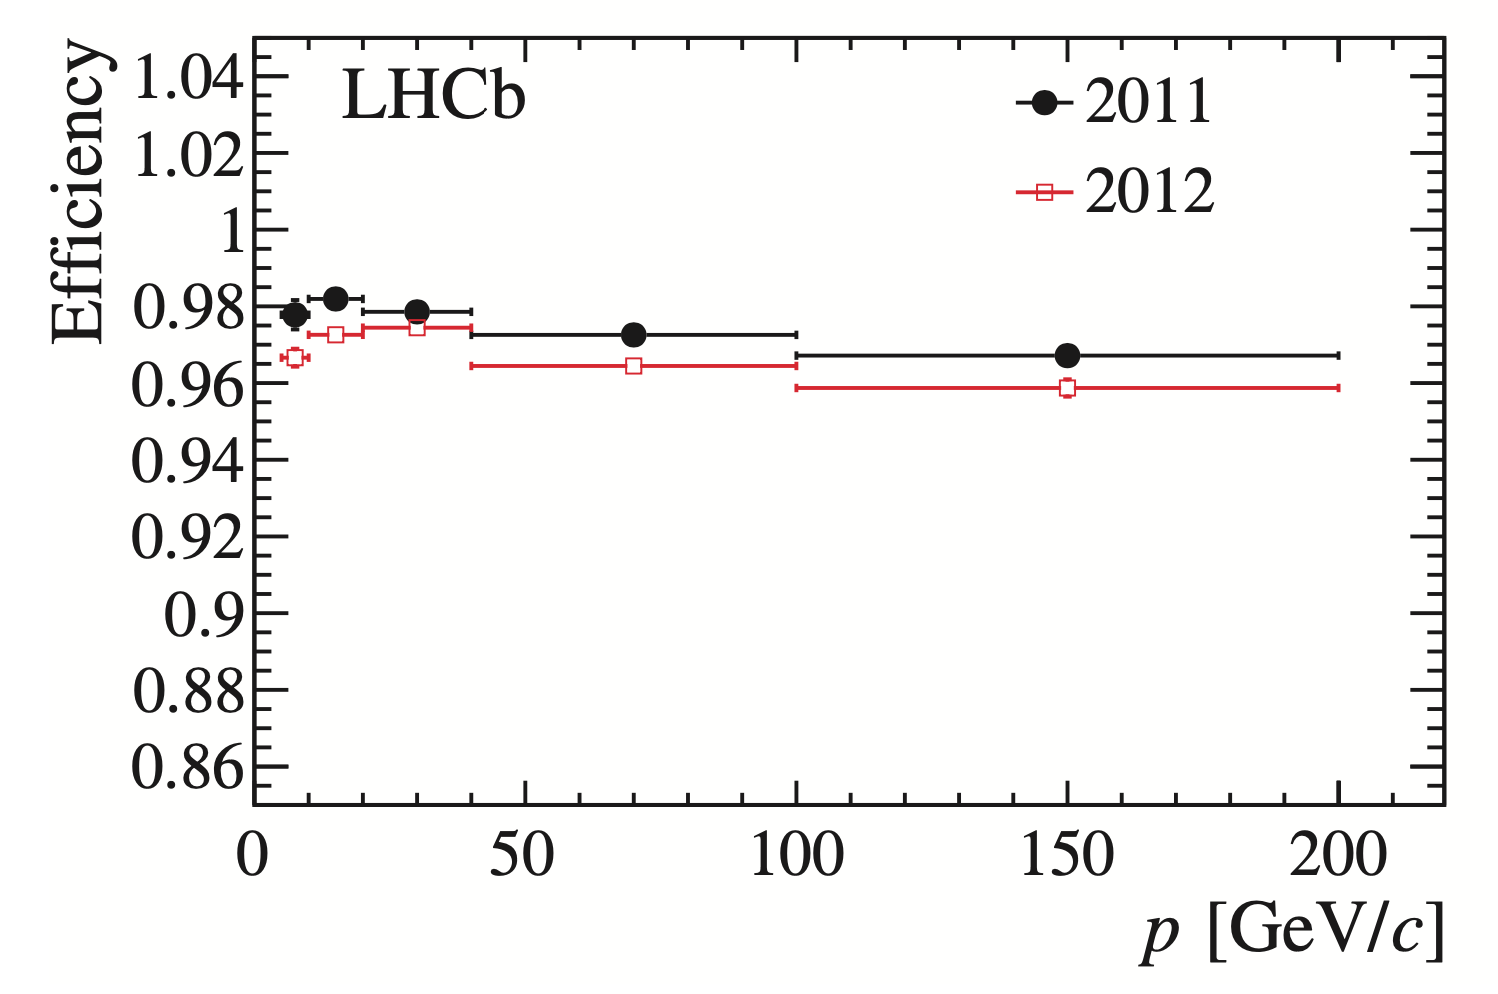
\includegraphics[width=0.45\columnwidth]{figures/detector/track_eff_p.png}
    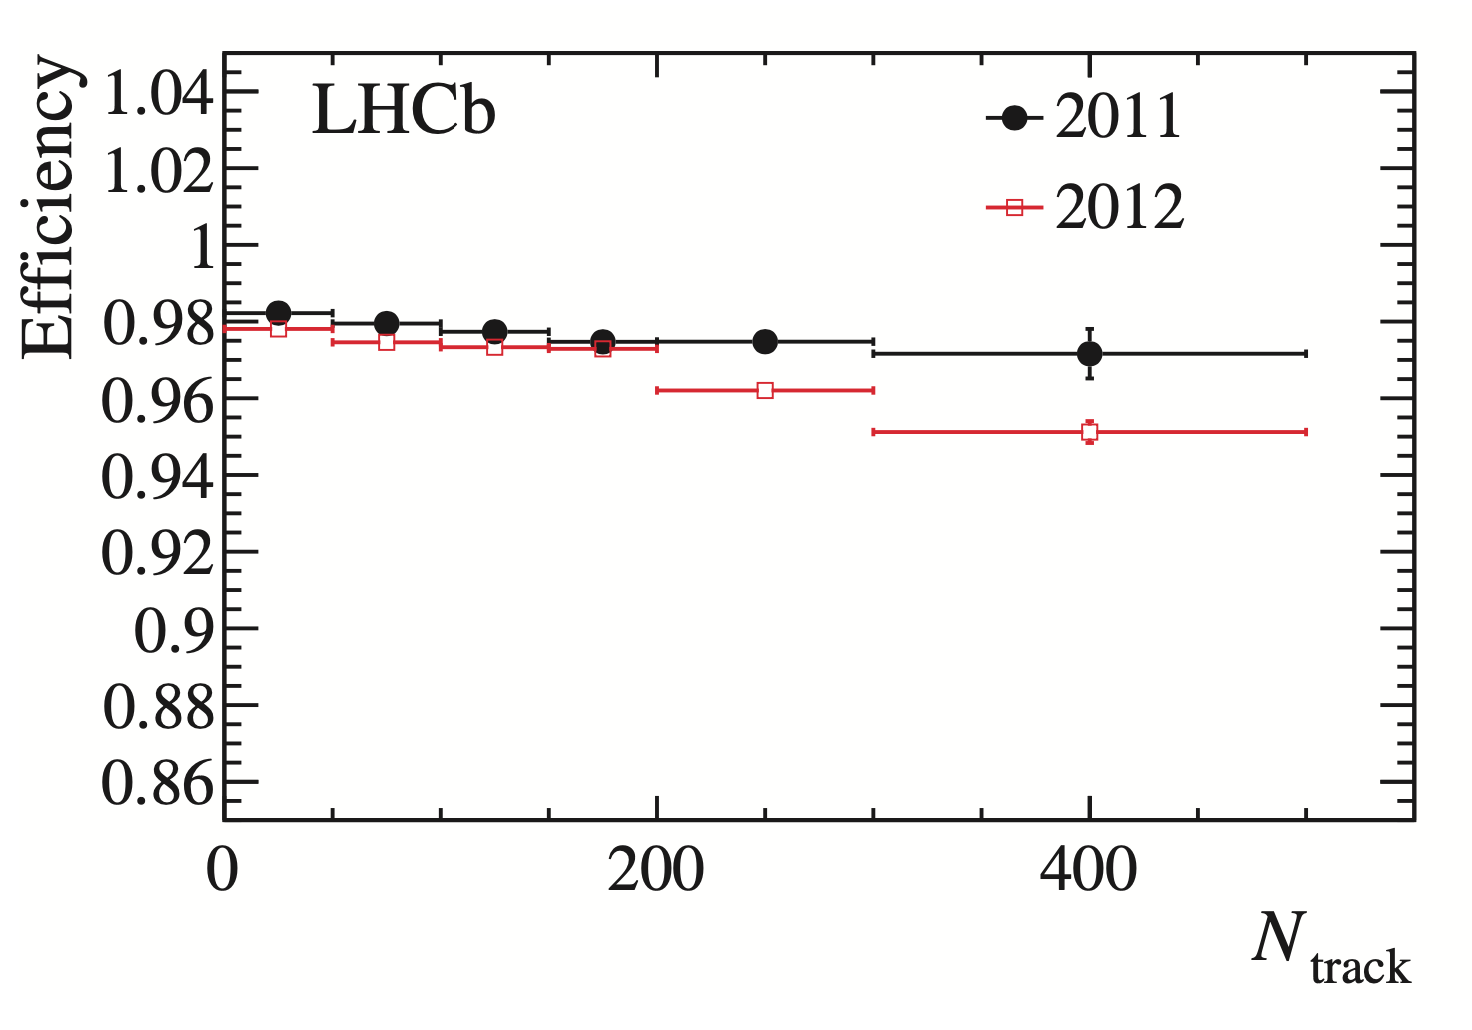
\includegraphics[width=0.45\columnwidth]{figures/detector/track_eff_N.png}
    \caption{The long track reconstruction efficiency as a function of (left) track momentum and (right) the number of charged tracks in the event. The figure is reproduced from Ref.~\cite{LHCb-Performance}.}
    \label{fig:track_eff}
\end{figure}

Many of the interesting signal decay channels of \lhcb have 4--6 charged final state tracks, and therefore it is crucial to have a single-track reconstruction efficiency close to 100\,\%. The single-track reconstruction efficiency is shown in Fig.~\ref{fig:track_eff} as a function of track momentum and the number of tracks in an \emph{event} (an \emph{event} denotes a $pp$ collision and all the particles produced therein and in subsequent decays). The efficiencies have been obtained in data, using a tag-and-probe method in $J/\psi\to\mup\mu^-$ decays~\cite{TrackEff}. One muon, the \emph{tag}, is fully reconstructed, while the other, the \emph{probe} is only partially reconstructed, allowing for the $J/\psi$ invariant mass to be reconstructed with reasonable resolution. If the partially reconstructed probe track is matched to a full long track, the track is classified as efficient.
Similar efficiencies have been achieved in Run~2.




\subsection{Particle identification} % (fold)
\label{sub:particle_identification}
The information from the RICH detectors, the calorimeters, and the muon system is generally combined, for optimal identification of charged tracks as electrons, muons, pions, kaons, or protons. Photons and neutral pions are identified using the ECAL, but play no role in the thesis, and will not be discussed further.

\begin{figure}[tb]
    \centering
    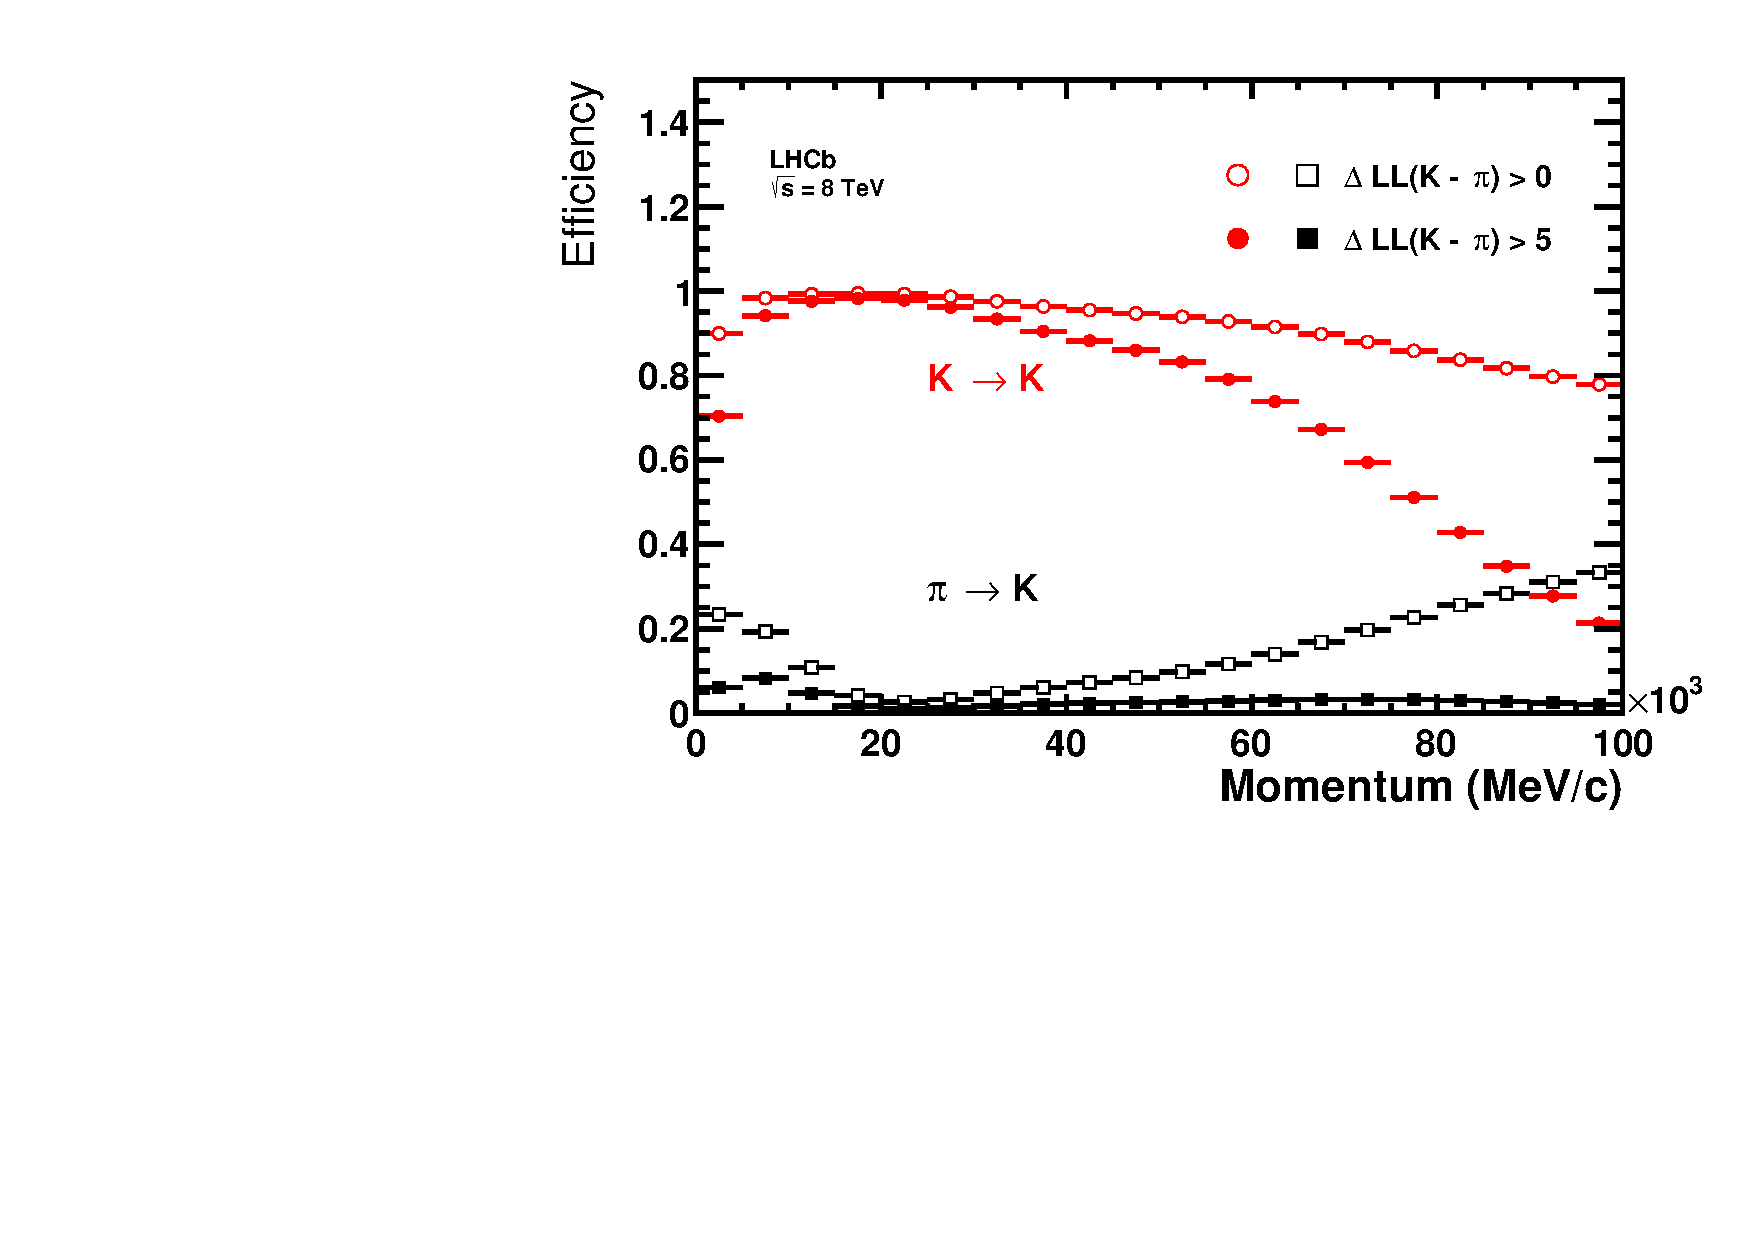
\includegraphics[width=0.45\columnwidth]{figures/detector/PIDK_Run1.pdf}
    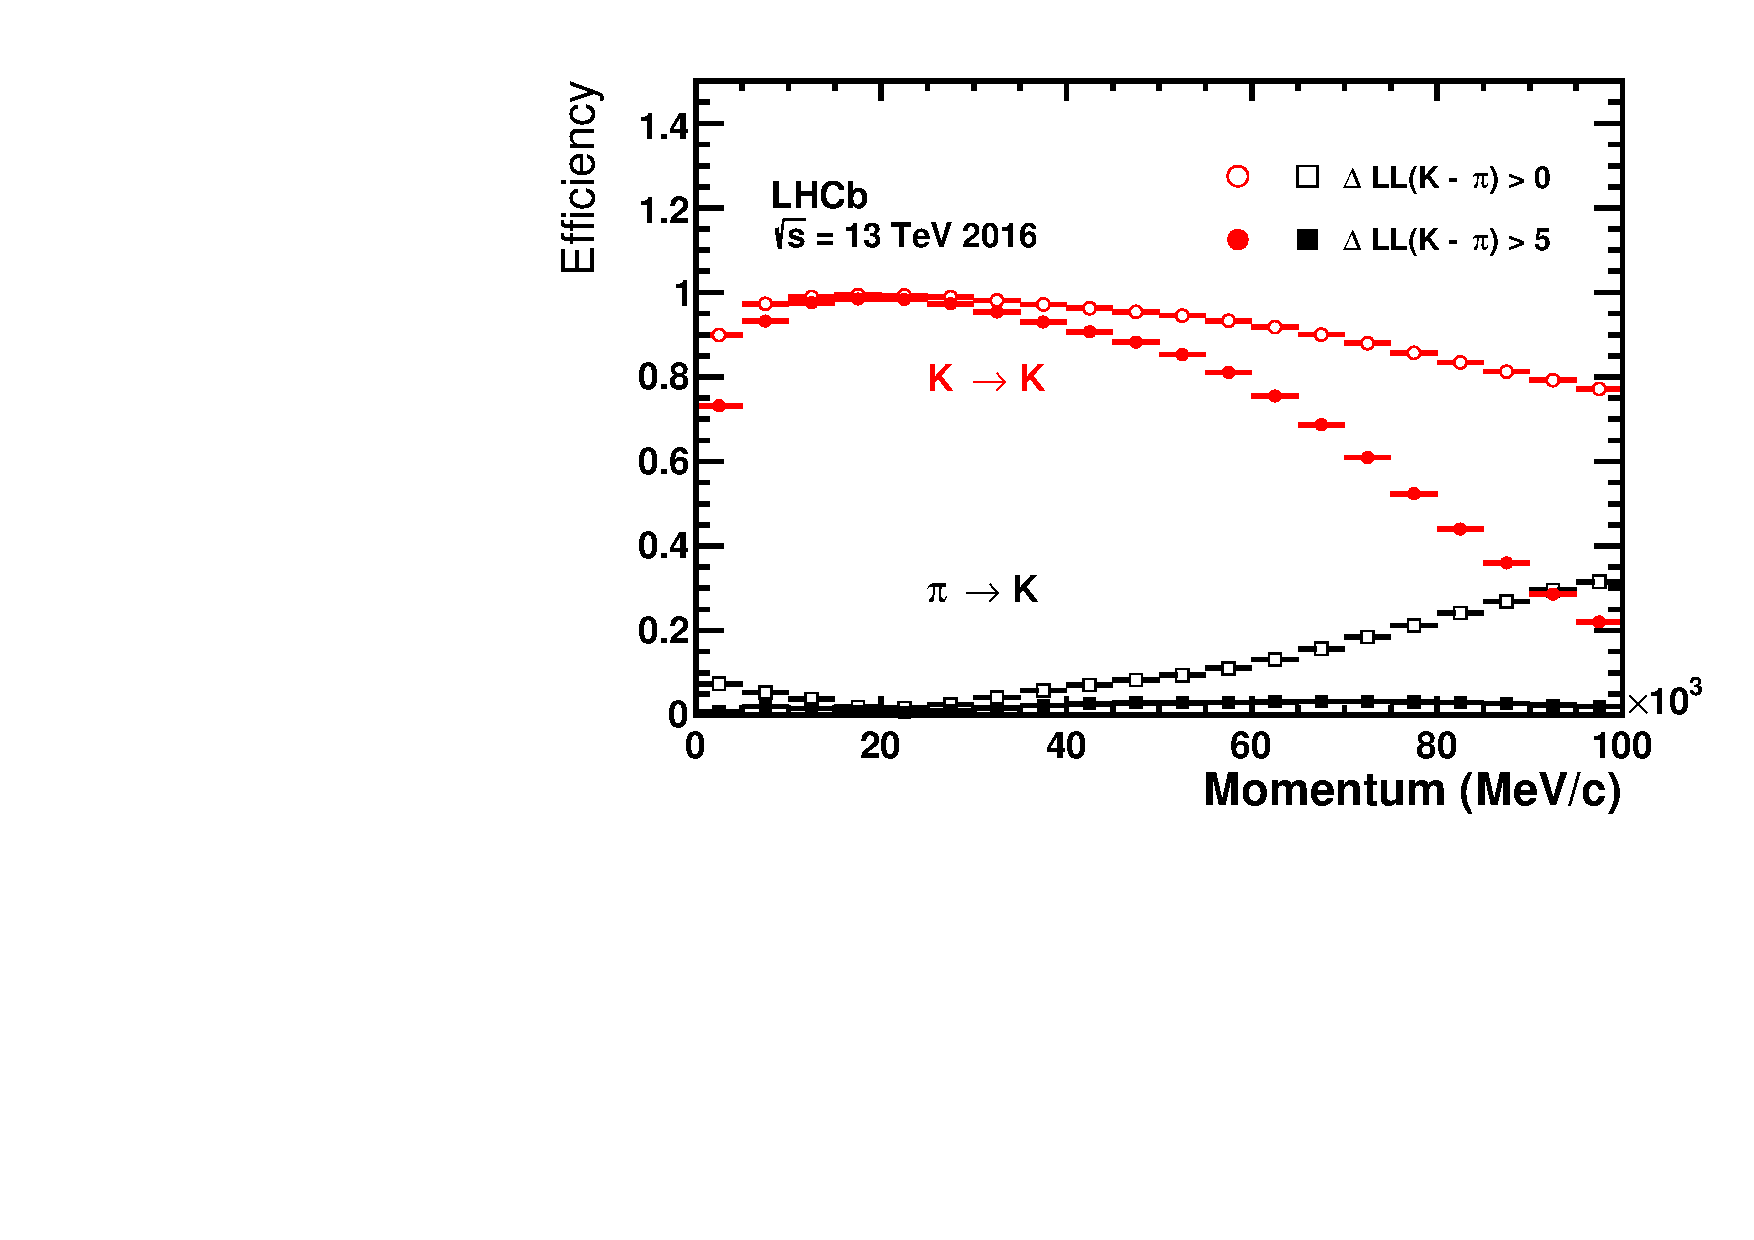
\includegraphics[width=0.45\columnwidth]{figures/detector/PIDK_Run2.pdf}
    \caption{The probability to correctly identify a kaon/misidentify a pion as a kaon given two different requirements on $\Delta LL(K)$, as a function of track momentum in (left) Run~1 data from 2012 and (right) Run~2 data from 2016. Reproduced from Ref.~\cite{PIDplots}.}
    \label{fig:PID_performance}
\end{figure}

The ability to separate \BtoDK and \BtoDpi decays is essential to the measurement presented in this thesis. In \lhcb, hadron separation is achieved via information from the RICH detectors, using a likelihood method where the observed pattern of hit pixels in the photo detectors is compared to the expected pattern, given all reconstructed tracks in an event under a given set of particle hypothesis. The likelihood is maximised by varying the particle hypotheses for each track being an electron, muon, pion, kaon, or proton~\cite{Forty:684714}.  It is necessary to consider all tracks of an event simultaneously because the Cherenkov rings of different tracks overlap. For each track, the maximum log likelihood of a particle hypothesis, say that the track is a kaon, relative to the hypothesis that it is a pion
\begin{align}\label{eq:DLL}
    \Delta\text{LL}_{\text{track}_i}^\text{RICH}(K) =  \ln \mathcal L_\text{max}^\text{RICH}(\text{pattern}|\text{track}_i = K)\ - \ln \mathcal L_\text{max}^\text{RICH}(\text{pattern}|\text{track}_i = \pi),
\end{align}
is saved to inform PID decisions. In the case of pion-kaon separation, this variable alone is enough to achieve good separation power; in the remainder of the thesis it is denoted \texttt{PIDK}. The PID performance for pion-kaon separation has been measured in calibration data, following a procedure described in Section~\ref{sub:efficiency_of_the_pid_requirements}, and is illustrated in Fig.~\ref{fig:PID_performance}.

\begin{figure}[tb]
    \centering
    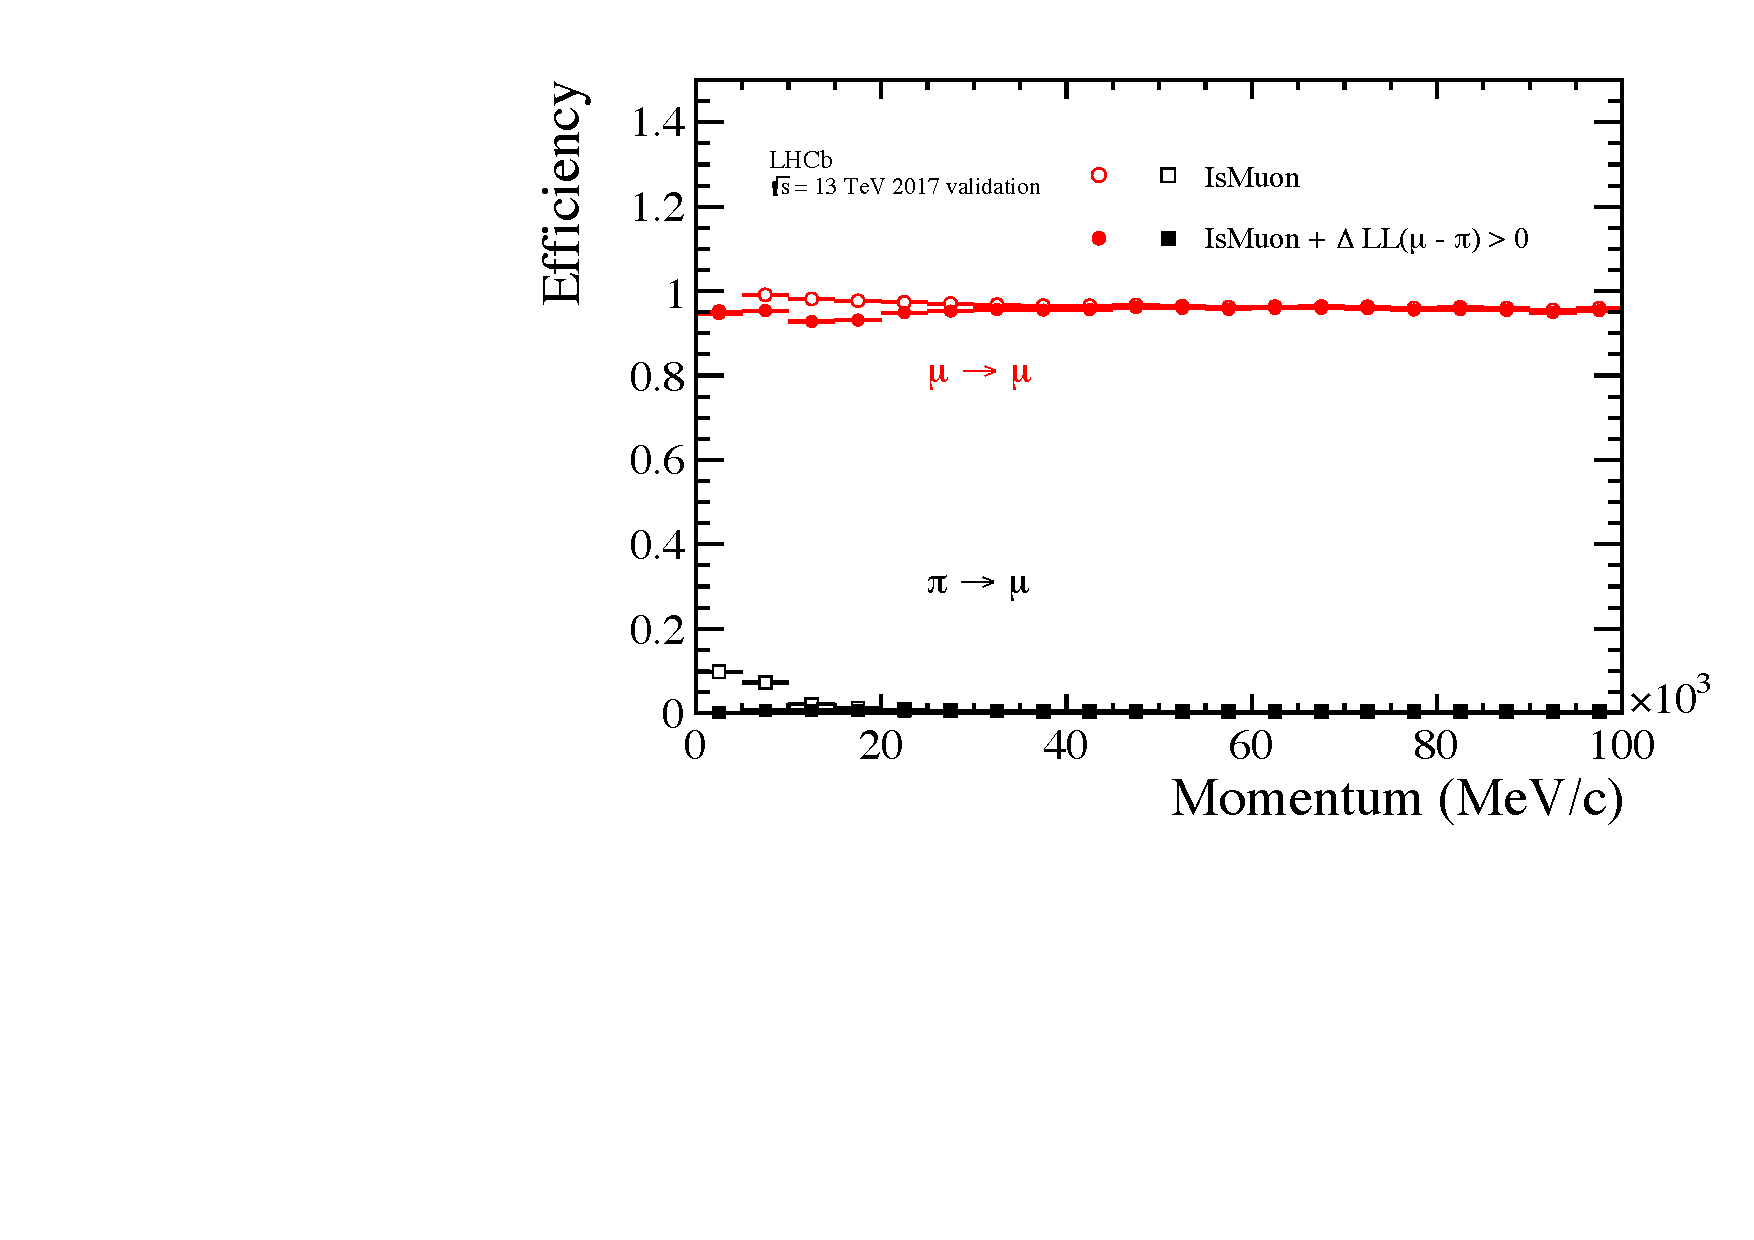
\includegraphics[width=0.60\columnwidth]{figures/detector/PIDmu_Run2.pdf}
    \caption{The probability to correctly identify a muon/misidentify a pion as a muon given requirements on either \texttt{isMuon} or $\Delta LL(\mu)$, as a function of track momentum in Run~2 data from 2017. Reproduced from Ref.~\cite{PIDplots}.}
    \label{fig:PIDmu_performance}
\end{figure}

Muons are identified by extrapolating tracks to the muon stations to define fields-of-interest (FOI). A track is considered as a muon candidate when a minimum number of stations (2--4 depending on the track momentum) have hits in the corresponding FOI~\cite{MuonPID,MuonPID2}. This information is encoded in a variable denoted \texttt{isMuon} throughout the thesis. Additional information, such as a comparison of the slopes of the track in the main tracker and the muon stations, and the average track-hit distance in the FOI is used to form a $\Delta \text{LL}^\text{muon}(\mu)$ variable analogous to the one defined in Eq.~\eqref{eq:DLL} for the RICH detectors; it can be combined with $\Delta \text{LL}^\text{RICH}(\mu)$ to form a PID variable that takes information from both detectors into account, denoted \texttt{PIDmu}. The performance of the muon PID variables is shown in Fig.~\ref{fig:PIDmu_performance} as obtained in data. It can be seen that requiring $\texttt{isMuon=0}$ rejects muon tracks efficiently at all momenta; this is used in the analysis to veto a number of semi-leptonic backgrounds.

In similar manner, a potential semi-leptonic background with electrons is also vetoed in the analysis presented in the thesis. In \lhcb, electron PID is mainly based on the balance between deposited energy and track momentum in the ECAL~\cite{ElectronPID}. This information is combined with information on photon deposits from brehmstrahlung, and energy deposits in the PS and HCAL, as well as information from the RICH and muon detectors, to form yet another $\Delta\text{LL}$ variable, denoted \texttt{PIDe}. As an example of the obtainable performance, an average electron selection effiency of $(91.9\pm1.3$\,\% was achieved in displaced $J/\psi\to e^+e^-$ decays in Run~1, with a hadron misidentification rate of $(5.54\pm0.02)$\,\%~\cite{LHCb-Performance}.

% subsection particle_identification (end)

% section reconstruction (end)

\section{The LHCb trigger system} % (fold)
\label{sec:the_lhcb_triggerring_system}

\begin{figure}[tb]
    \centering
    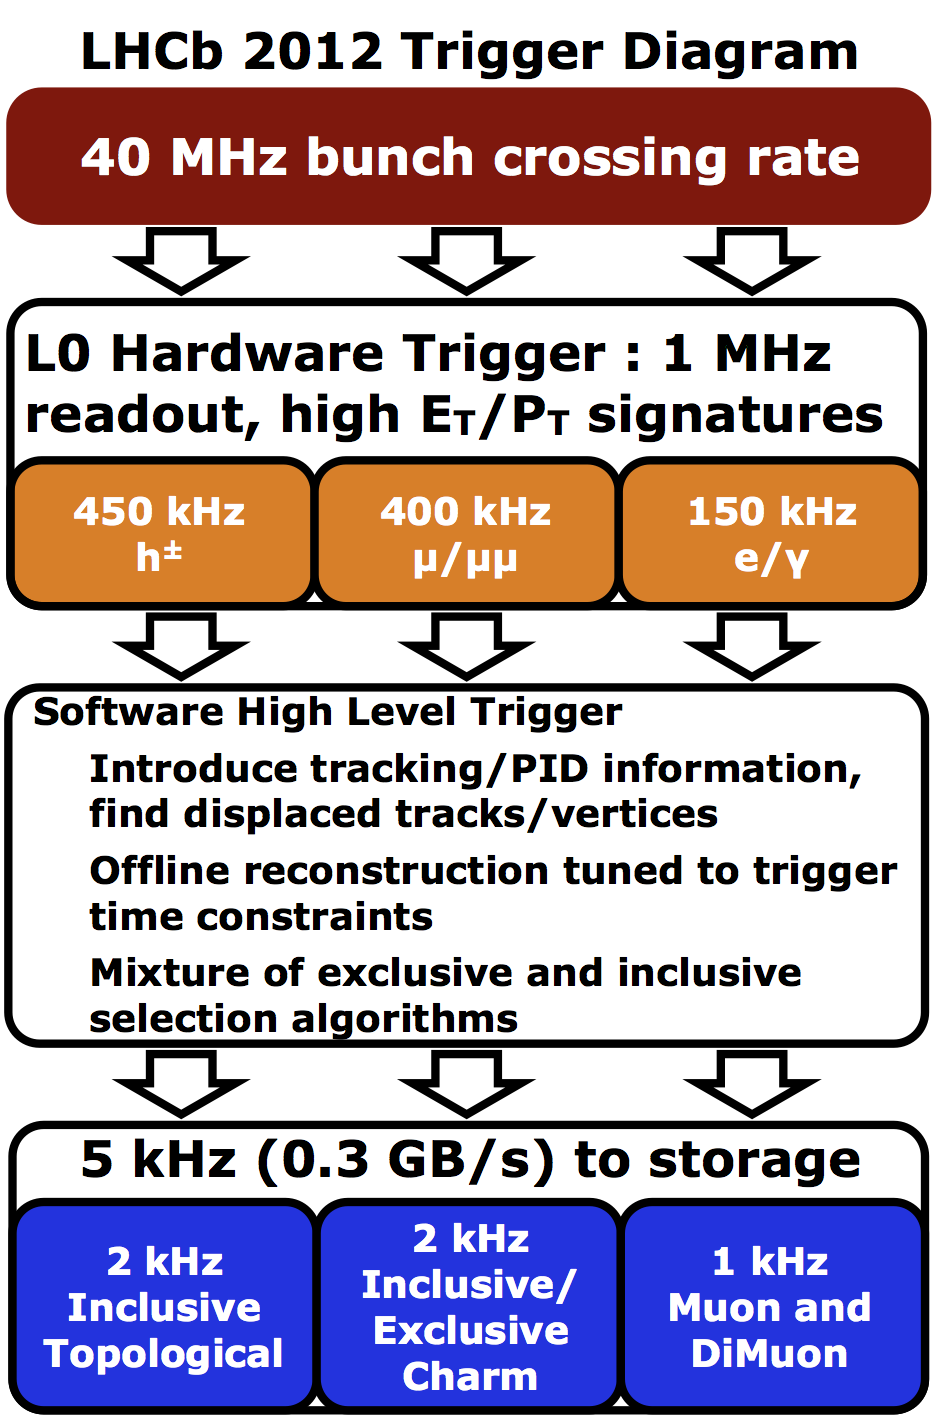
\includegraphics[width=0.45\columnwidth]{figures/detector/Trigger_Run1.png}\hspace{1cm}
    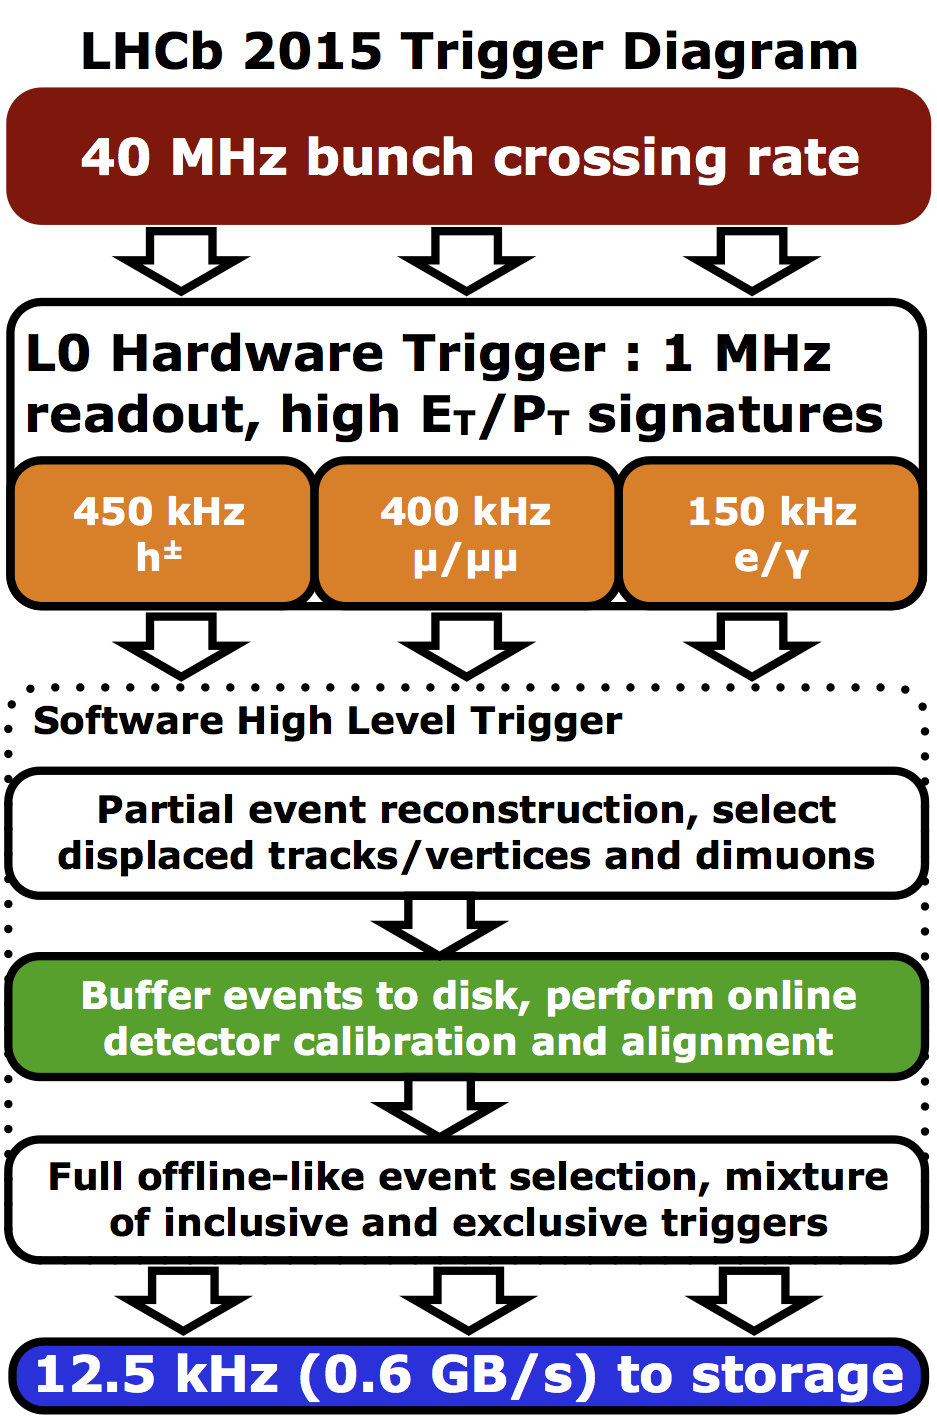
\includegraphics[width=0.45\columnwidth]{figures/detector/Trigger_Run2.png}
    \caption{Illustration of stages and event processing rates in the \lhcb trigger during (left) Run~1 and (right) Run~2. }
    \label{fig:trigger_stages}
\end{figure}

The collision rate in the LHC is up to 40\,MHz, with a visible inelastic collision rate in \lhcb of up to 30\,MHz. The \lhcb uses a multi-stage trigger to reduce rate with which events are stored to a manageable level (of eg. 12.5\,kHz during Run~2). The first stage consists of a hardware trigger that selects events with high transverse energy in the calorimeters, or hits in the muon detectors. This is followed by two software stages that rely on a reconstruction of tracks in the detector to select events that are likely to include interesting physics.  The overall trigger stages were identical in Run~1 and Run~2, however the throughput rate was upgrade significantly between the two data taking period, as was the quality of the reconstruction in the software trigger stages; in Run~2, the final software trigger decisions are in fact based on the full offline event reconstruction~\cite{Trigger-Performance2}.  The stages are illustrated in Fig.~\ref{fig:trigger_stages}, and described in detail in the following.

A further, offline processing and reconstruction step is applied to all events before they are made available to most \lhcb analyses, commonly denoted as the \emph{stripping} step. Although the stripping does not form part of the \lhcb trigger, it does constitute an additional, centralised filter on the data, and a description is included in Section~\ref{sub:offline_data_filtering_the_lhcb_stripping}.



\subsection{The level-0 hardware trigger} % (fold)
\label{sub:the_level_0_hardware_trigger}

The level-0 (L0) triggers that select physics events are based on the calorimeters and the muon system. 
The ECAL and HCAL are divided into clusters of $2\times2$ cells, for which the transverse energy is defined as
\begin{align}
    E_T=\sum_{j} E_j \sin \theta_j,
\end{align}
where $\theta_j$ is the angle of cell $j$ with respect to the beam axis and the average collision point. The trigger forms a \texttt{L0Hadron} candidate with the highest $E_T$ found in the HCAL, combined with the ECAL cluster in front of it if such a cluster is present. Photon and electron candidates are formed based on clusters in the ECAL, identified by the presence (lack) of hits in the SPD for an elentron (photon). The transverse energies of the candidates are compared to a fixed set of thresholds, and events where at least one candidate is above threshold are retained.

The muon trigger searches for straight line tracks in the muon stations, estimating the associated muon $p_T$ based on the track direction. An event is retained is either the largest muon $p_T$ is above a given threshold, or the product of the two highest muon $p_T$ values is above a different threshold.

High-multiplicity events take a long time to process in the subsequent software stage; therefore it is favourable for the overall retention rate of interesting physics decays to put a maximum limit on the event multiplicity at the L0 stage. This is achieved by requiring the number of hits in the SPD detector to be below a threshold value in most L0 lines.

% subsection the_level_0_hardware_trigger (end)

\subsection{High-level triggers} % (fold)
\label{sub:high_level_triggers}

The events that pass the L0 trigger are passed to a farm of multiprocessor computing node, the Event Filter Farm (EFF), tasked with bringing the rate down from approximately 1\,MHz to the $\mathcal O(1-10)$\,kHz rate that can be saved to disk. The EFF consisted of 900 (1700) nodes during Run~1 (Run~2). The software-based filtering proceeds in two stages: a first filter (HLT1) brings the rate down to approximately 40\,(110)\,kHz based on a limited reconstruction of the event,  after which a second stage  (HLT2) filters the events further based on a more complete reconstruction. Each step executes a number of different algorithms, each of which can allow an event to be accepted; these are denoted \emph{trigger lines.}

During both runs, the HLT1 performed a partial event reconstruction by building long tracks that satisfy a $p_T$ requirement using the forward tracking approach described in Section~\ref{sub:track_reconstruction}, and determining the location of PVs using VELO tracks. In both runs, the HLT1 included an inclusive trigger that selected a high $p_T$ track with significant displacement of all PVs (typical of a $b$ or $c$ decay). This line is denoted \texttt{HLT1TrackAllL0} in Run~1~\cite{Trigger-Performance}; for Run~2 the track requirements were reoptimised and it is denoted \texttt{Hlt1TrackMVA}. Further, an additional inclusive trigger was added that forms a two-prong vertex out of high $p_T$ tracks inconsistent with originating in a PV, and applies a multivariate classifier to determine if it is signal-like based on a number of track and vertex properties. This line is denoted \texttt{Hlt1TwoTrackMVA}~\cite{Trigger-Performance2}. These lines triggered all events included in the analysis of the thesis; other lines exist for selecting events that include muons, calibration data, low-multiplicity events, and a number of exclusive lines, for a total of approximately 20 lines during Run~2~\cite{Trigger-Performance2}.

Because the rate of events is reduced significantly by HLT1, the HLT2 decisions can be based in a more complete reconstruction of the event. Indeed, during Run~2 it was based on a complete, fully aligned reconstruction equivalent to the offline reconstruction. During Run~1 the HLT2 reconstruction only included long tracks and did exclude some low momentum tracks; this was a main motivation for the upgrade of the EFF during the shutdown period. The need for full alignment in HLT2 means that is could not be run fully online in Run~2; instead the output events were saved to disk in the EFF, and processed with some delay~\cite{Trigger-Performance2}. The analysis presented in the thesis is based on a number of inclusive "topological" trigger lines, based on combinations of 2, 3, or 4 tracks that satisfy fit quality requirements, have high $p_T$, are separated from the PVs, and have a distance-of-closes-approach below 0.2\mm. A multivariate classifier~\cite{gligorovEfficientReliableFast2013} is applied to each formed $n$-body object, to determine if the event should be accepted based on the track momenta, invariant mass, a corrected invariant mass that takes into account missing transverse momentum, distance of closest approach, and the impact parameter and separation with the associated PV. The resulting trigger lines were denoted \texttt{Hlt2Topo\{2, 3, 4\}BodyBBDT} during Run~1 and \texttt{Hlt2Topo\{2, 3, 4\}Body} during Run~2.  A large number of other HLT2 lines exist (more than 500 in Run~2), including a significant number of exclusive lines that aim to select specific decays and only save information on the signal decay, not the whole event. This was made possible by the full reconstruction within HLT2~\cite{Trigger-Performance2}, and have allowed for larger signal yields to be collected within the data storage limits.

% subsection high_level_triggers (end)

\subsection{Offline data filtering: the \lhcb stripping} % (fold)
\label{sub:offline_data_filtering_the_lhcb_stripping}

Events that are written to disk are processed with the full detector alignment and calibration. In a further, offline processing step denoted the \emph{stripping}, hundreds of different, dedicated reconstructions are performed; decay candidates for various signal decays are built and a number of requirements are made to reject backgrounds from random track combinations. For example, the $\Bpm\to\D(\to\KS h'^+h'^-)h^\pm$ candidates that are analysed in this thesis are built during the stripping stage, as described further in Section~\ref{sec:candidate_selection}. The stripping is a centralised computing task, executed on the Worldwide LHC Computing Grid~\cite{birdComputingLargeHadron2011a}, and allows the analysts to process much smaller data sets during their individual analysis. Because the stripping is based on data saved to offline storage it can be repeated; however, the processing of data collected during a year of data taking takes many weeks, so this does not happen often.

% subsection offline_data_filtering_the_lhcb_stripping (end)

% section the_lhcb_triggerring_system (end)



\section{Simulation} % (fold)
\label{sec:simulation}

A centralised \lhcb simulation is able to simulate $pp$ collisions with the proper conditions within \lhcb, subsequent secondary decays, and the detector response, and process it via the full \lhcb reconstruction. In this thesis, simulated decays are used to determine the reconstructed invariant-mass distribution of a number of decay modes, as well as a number of relative selection efficiencies. The $pp$ collisions are generated using \pythia~\cite{Sjostrand:2007gs,*Sjostrand:2006za} with a specific configuration specific to \lhcb~\cite{LHCb-PROC-2010-056}. The time-dependent evolution and decays of unstable particles are described by the \evtgen~\cite{EvtGen} package, designed specifically for \B physics. Final-state radiation is generated using \photos~\cite{Golonka:2005pn}. The interaction of the generated particles with the detector, and its response, are implemented using the \geant toolkit~\cite{Allison:2006ve, *Agostinelli:2002hh} as described in  Ref.~\cite{LHCb-PROC-2011-006}. 

The most significant computational cost of the simulation is due to the detector simulation. A single $pp$ collision produces $\mathcal O(100)$ tracks in the detector, out of which only a handful belong to the signal decay under study. Therefore, significant computation resources can be saved by reusing the detector simulation of non-signal tracks a number of times, while redecaying the signal particle, say a \Bp, each time. This approach is called ReDecay~\cite{LHCb-DP-2018-004}, and has been relatively widely adopted within \lhcb. ReDecay has been used to produce simulation samples corresponding to the conditions in 2017 and 2018 for this thesis. In some cases, the use of ReDecay necessitates special statistical treatment due the correlated detector occupancies between signal candidates, but for the analysis in this thesis the impact is negligible.

A number of sub-dominant backgrounds are investigated using the fast-simulation package \texttt{RapidSim}~\cite{cowanRapidSimApplicationFast2017}. This package can decay heavy $b$ and $c$ hadrons with kinematic distributions similar to those in \lhcb $pp$ collisions, or with user defined input distributions. The decays are typically evenly distributed over phase space, but can also be handled with \evtgen~\cite{EvtGen} to take involved spins and resonant structure into account. Furthermore, a smearing of the obtained momenta is implemented, based on the \lhcb resolution. 

% subsection rapidsim_a_fast_simulation_tool (end)RapidSim.

% section simulation (end)
% \begin{savequote}[8cm]
% Alles Gescheite ist schon gedacht worden.\\
% Man muss nur versuchen, es noch einmal zu denken.

% All intelligent thoughts have already been thought;\\
% what is necessary is only to try to think them again.
%   \qauthor{--- Johann Wolfgang von Goethe \cite{von_goethe_wilhelm_1829}}
% \end{savequote}

\chapter{\texorpdfstring{Neutral kaon \CP violation and material\\interaction in BPGGSZ measurements}{Neutral kaon CP violation and material interaction in BPGGSZ measurements}}
\label{ch:4-KS-CPV}

The presence of a \KS meson in the $\D\to\KS h^+h^-$ final states introduces a small bias in BPGGSZ measurements due to \CP-violation in the neutral kaon sector and asymmetries caused by the interaction between the neutral kaon and detector material. These fundamental physics effects are reviewed in Section~\ref{sec:cp_violation_and_material_interaction_of_neutral_kaons}, after which the chapter presents a detailed analysis of the impact on the \lhcb measurement that is the subject of the thesis,  as well as future $\gamma$ measurements with the Belle II experiment. 
Prior to this analysis, the only existing work on the the effect on $\gamma$ measurements suggested a small effect in \BtoDK measurements but potentially \emph{very} significant effects in measurements based on \BtoDpi decays~\cite{grossmanEffectsBarMixing2014}. However, as described in Section~\ref{sub:a_first_look_at_the_impact_on_gamma}, the analysis in Ref.~\cite{grossmanEffectsBarMixing2014} does not take into account the fundamental aspect of the BPGGSZ method: that it relies on the phase-space distribution of signal decays, not phase-space-integrated asymmetries. Furthermore, the earlier study only considers the \CP-violation effect, not material interaction. Therefore, a more detailed study was necessary before the \BtoDpi decay mode could reliably be promoted to a signal channel. The full analysis shows the impact on the $\gamma$ measurement in Chapter~\ref{ch:5-GGSZ-measurement} to be small, and allows for the assignment of an appropriate systematic uncertainty.



\section{CP violation and material interaction of neutral kaons} % (fold)
\label{sec:cp_violation_and_material_interaction_of_neutral_kaons}

A brief review of the general phenomenology of mixing and \CP violation in the neutral kaon system is useful, before analysing the impact on $\gamma$ measurements. The presentation in this section follows the PDG review of \emph{\CP violation in the quark section}~\cite{PDG2020}. The general theory considers any pair of neutral meson states $\ket \Mz$ and $\ket \Mzb$ related by \CP conjugation
\begin{subequations}
\begin{align}
     \CP \ket \Mz  &= e^{i\phi_M} \ket \Mzb     &
     \CP \ket \Mzb &= e^{-i\phi_M}\ket \Mz ,
 \end{align} 
 where $\phi_M$ is an arbitrary phase. In this thesis, the convention $\phi_M=0$ is chosen, so that
 \begin{align}\label{eq:CP_convention}
     \CP \ket \Mz  &= \ket \Mzb     &
     \CP \ket \Mzb &= \ket \Mz.
 \end{align}
 \end{subequations}
A meson state that starts as a general superposition of $\ket \Mz$ and $\ket \Mzb$ states
\begin{align}
\begin{split}
       \psi_M^0\equiv \psi_M(0) &= a(0)\ket \Mz + b(0)\ket \Mzb \\&\equiv \psi_{\Mz}^0 + \psi_{\Mzb}^0
    \end{split}
\end{align}
will, over time, evolve into a state that consists of a different superposition of $\ket \Mz$ and $\ket \Mzb$, as well as components for all possible states the meson system can decay into
\begin{align}
\begin{split}
     \psi_M(t) &= a(t)\ket \Mz + b(t)\ket \Mzb + \sum c_i(t) f_i \\&\equiv \psi_{\Mz}(t) + \psi_{\Mzb}(t) + \sum c_i(t) f_i.
\end{split}
 \end{align} 
 For time scales that are longer than the typical strong-interaction, the time evolution of the \Mz--\Mzb superposition can be described by a $2\times 2$ Hamiltonian
 \begin{align}
      \frac{\text d}{\text dt} \begin{pmatrix}\psi_{\Mz}(t)\\\psi_{\Mzb}(t)\end{pmatrix} = -i\mathcal H_0 \begin{pmatrix}\psi_{\Mz}(t)\\\psi_{\Mzb}(t)\end{pmatrix}
  \end{align} 
 that is \emph{non-Hermitian} (to allow for decay) but can be parameterised in terms of two Hermitian matrices $\mathcal M$ and $\Gamma_0$
 \begin{align}
     \mathcal H_0 = \mathcal M - \frac{i}{2}\Gamma_0.
 \end{align}
 The quantum states with well-defined (real) masses, $m_j$, and (real) decay widths, $\Gamma_j$, are the two eigenstates of $\mathcal H_0$ with eigenvalues $\lambda_j = m_j - \frac{i}{2}\Gamma_j$. The eigenstates (of course) evolve independently in time, so that
 \begin{align}\label{eq:vac_time_dep}
     \psi_j(t) &= e^{-i\lambda_{j}t} \psi_{j}^0 =  e^{-im_{j}t -\frac{\Gamma_{j}}{2}t}\psi_{j}^0.
 \end{align}
 The eigenstates are denoted $H$ and $L$  according to the size of $m_j$, the real part of the eigenvalues, such that $m_H > m_L$. 
 Assuming that $\mathcal H_0$ conserves $CPT$ the eigenstates have the general form
 \begin{align}
 \begin{split}\label{eq:general_pq_form}
     \ket {M_H} &\equiv p \ket\Mz - q \ket \Mzb \\
     \ket {M_L} &\equiv p \ket\Mz + q \ket \Mzb 
 \end{split}
 \end{align}
where $p$ and $q$ are complex numbers that satisfy $|q|^2+|p|^2=1$.
%\footnote{Since $\mathcal H_0$ is non-Hermitian, the eigenstates are not, generally, orthogonal.} 
With the convention in Eq.~\eqref{eq:CP_convention} it follows that \emph{if} $\mathcal H_0$ also conserves \CP, so that $\ket {M_H}$ and $\ket {M_L}$ are \CP eigenstates, then $p=\pm q$, where the sign depends on which of the heavy and the light meson states is \CP even, and which is \CP odd.



The eigenstates of the Hamiltonian governing the neutral kaon system are almost, but not exactly, equal to the \CP eigenstates
\begin{align}\label{eq:K_CP_states}
    \ket{K_1}   &= \frac{\ket \Kz + \ket \Kzb}{\sqrt{2}} &
    \ket{K_2}   &= \frac{\ket \Kz - \ket \Kzb}{\sqrt{2}},
\end{align}
which are \CP even and odd, respectively. This approximate equality leads to the most prominent feature of the neutral kaon system: the two eigenstates of $\mathcal H_0$ have lifetimes that differ by orders of magnitude. This is best understood by assuming, for a moment, that the states in Eq.~\eqref{eq:K_CP_states} \emph{do} equal the eigenstates with definite life times. The $K_1$ state can decay in the \CP even $\pip\pim$ and $\piz\piz$ modes, and does so almost 100\,\% of the time; these decay modes are not available to the $K_2$ (in the absence of direct \CP violation) which results in a much lower decay rate and a much longer life time. Therefore, the eigenstates in the kaon system are labelled the \emph{short-lived} kaon, \KS, which is almost \CP even, and the \emph{long-lived} kaon, \KL, which is almost \CP odd. The life times are~\cite{PDG2020}
\begin{align}
    \tau_\KS &= (8.954\pm0.004)\times10^{-11} \text s &
    \tau_\KL &= (5.116\pm0.021)\times10^{-8} \text s.
\end{align}
Experimentally, it is found that the \KS corresponds to the light eigenstate, but that the mass splitting~\cite{PDG2020}
\begin{align}
\begin{split}
    \Delta m = m_\KL-m_\KS &= (0.5289\pm0.0009)\times 10^{10} \,\hbar \text s^{-1}\\
    &\simeq 3.5\times 10^{-6} \ev
\end{split}
\end{align}
is tiny compared to the neutral kaon masses of $m_\KS=497.6\mevcc$~\cite{PDG2020}.

However, the discovery of $\KL\to\pi\pi$ decays by Kronin and Fitch in 1964 established that the \KS and \KL are \emph{not} exactly equal to the \CP eigenstates in Eq.~\eqref{eq:K_CP_states}, because the $\mathcal H_0$ relevant to the kaon system is \CP-violating. The \CP violation in the kaon sector is conventionally parameterised in terms of the complex parameters $\epsilon$ and $\epsilon'$, in terms of which
\begin{align}
    \frac{A(\KL\to\pip\pim)}{A(\KS\to\pip\pim)} &= \epsilon + \epsilon' &
    \frac{A(\KL\to\piz\piz)}{A(\KS\to\piz\piz)} &= \epsilon -2 \epsilon'. 
\end{align}
In these expressions $\epsilon$ denotes the contribution from \CP violation in mixing and $\epsilon'$ the contribution due to direct \CP violation in the decays.  The $\epsilon$ parameter has been measured to be~\cite{PDG2020}  
\begin{align}\label{eq:PDG_epsilon}
    |\epsilon|=(2.228\pm 0.011)\times 10^{-3}, \qquad \arg \epsilon = (43.52\pm 0.05)^\circ,
\end{align}
while the $\epsilon'$ parameter satisfies~\cite{PDG2020}
\begin{align}
  \text{Re}(\epsilon'/\epsilon)\simeq \epsilon'/\epsilon \simeq (1.66\pm0.23)\times 10^{-3}
\end{align}
Direct \CP violation is ignored for the remainder of the thesis, because $\epsilon'$ is measured to be three orders of magnitude smaller than $\epsilon$. In terms of the \CP eigenstates of Eq.~\eqref{eq:K_CP_states}, the mass eigenstates \KS and \KL are given by
\begin{align}
\begin{split}
    \ket{\KS}   &= \frac{\ket{K_1} + \epsilon \ket{K_2}}{\sqrt{ 1+|\epsilon|^2}} 
     \qquad= \frac{(1+\epsilon)\ket\Kz + (1-\epsilon)\ket\Kzb}{\sqrt{2(1+|\epsilon|^2)}} 
    \\
    \ket{\KL}   &= \frac{\ket{K_2} + \epsilon \ket{K_1}}{\sqrt{ 1+|\epsilon|^2}} 
     \qquad= \frac{(1+\epsilon)\ket\Kz - (1-\epsilon)\ket\Kzb}{\sqrt{2(1+|\epsilon|^2)}},
\end{split}
\end{align}
corresponding to the definition $p=(1+\epsilon)/\sqrt{2(1+|\epsilon|^2)}$ and $q=(1-\epsilon)/\sqrt{2(1+|\epsilon|^2)}$ in Eq.~\eqref{eq:general_pq_form}.



In an experimental setting, the time evolution of a neutral kaon state is affected by nuclear interactions with the detector. The interaction is governed by the strong force, and therefore sensitive to the \emph{flavour} of the kaon state; the interaction strength is thus different for \Kz and \Kzb mesons. This difference introduces a non-zero $\KS\leftrightarrow\KL$ transition amplitude for neutral kaons traversing a detector segment. This effect was predicted early in the history of kaon physics~\cite{paisNoteDecayAbsorption1955} and is commonly denoted \emph{kaon regeneration}. The effect can be described by including a material-interaction term in the Hamiltonian
that is diagonal in the $(\ket\Kz, \ket \Kzb)$ basis, so that the equation governing the time evolution is~\cite{goodRelationScatteringAbsorption1957,fetscherRegenerationArbitraryCoherent1996}
\begin{align}\label{eq:time_evol_K_with_mat}
      \frac{\text d}{\text dt} \begin{pmatrix}\psi_{\Kz}(t)\\\psi_{\Kzb}(t)\end{pmatrix} = -i\left[
      \mathcal H_0 + \begin{pmatrix}
          \chi & 0 \\ 0 & \bar \chi
      \end{pmatrix}
      \right]
      \begin{pmatrix}\psi_{\Kz}(t)\\\psi_{\Kzb}(t)\end{pmatrix}.
\end{align}
The complex parameters $\chi$ and $\bar\chi$ describe the material interaction of the \Kz and \Kzb flavour eigenstates and are related to their scattering cross section, as described further in Section~\ref{sub:detector_material_budget}. 
The solution of Eq.~\eqref{eq:time_evol_K_with_mat} for the time evolution in the \KS and \KL states is~\cite{fetscherRegenerationArbitraryCoherent1996}
\begin{align} 
\begin{split} \label{eq:mat_time_dep}
\psi_{\rm{S}}(t) &= e^{-i\Sigma t}\left( \psi^0_{\rm S}\cos \Omega t  
                + \frac{i}{2\Omega}\left(\Delta \lambda \psi^0_{\rm S} - \Delta \chi \psi^0_{\rm L}\right) \sin \Omega t \right) ,\\
\psi_{\rm{L}}(t) &= e^{-i\Sigma t}\left( \psi^0_{\rm L}\cos \Omega t  
                - \frac{i}{2\Omega}\left(\Delta \lambda \psi^0_{\rm L} + \Delta \chi \psi^0_{\rm S}\right) \sin \Omega t \right) ,
\end{split}
\end{align} in terms of the parameters
\begin{align} 
\begin{split}
 \label{eq:mat_param}
\Delta \chi &= \chi - \bar \chi, \\
\Delta \lambda &= \lambda_{\rm L} - \lambda_{\rm S} = (m_{\rm L} - m_{\rm S}) - \frac{i}{2}(\Gamma_{\rm L} - \Gamma_{\rm S}),
\\ 
 \Sigma & = \frac{1}{2}\left(\lambda_{\rm S} + \lambda_{\rm L} + \chi + \bar \chi\right), \\
 \Omega &= \frac{1}{2}\sqrt{\Delta \lambda^2 + \Delta \chi^2}.
\end{split}
\end{align}
In the vacuum limit where $\chi=\bar\chi=0$, the expressions in Eq.~\eqref{eq:vac_time_dep}~and~Eq.~\eqref{eq:mat_time_dep} are equal. 


\subsection{\texorpdfstring{A first look at the impact on $\gamma$ measurements}{A first look at the impact on gamma measurements}} % (fold)
\label{sub:a_first_look_at_the_impact_on_gamma}

% subsection a_first_look_at_the_impact_on_ (end)



The effects described above have an impact on measurements of \CP asymmetries in modes with a neutral kaon in the final state. This was analysed for the first time in relation to $\gamma$ measurements by Grossman and Savastio in 2014~\cite{grossmanEffectsBarMixing2014}. The authors point out two sources of corrections to be included:
\begin{itemize}
    \item the fact that \KS is not an exact \CP eigenstate can break potential symmetry relations employed in an analysis, and
    \item that when the neutral kaon is reconstructed in a $\pi\pi$ final state there will be contributions from both \KS and \KL decays.
\end{itemize}
The analysis in this chapter considers yet another effect, not treated by Grossman and Savastio, namely that
\begin{itemize}
  \item material interaction can emulate the effect of neutral kaon \CP violation, because it couples the almost-\CP-even \KS and the almost-\CP-odd \KL states.  
\end{itemize}
Due to the presence of $\KL\to\pi\pi$ decays, Grossman and Savastio point out that the relevant decay rates to consider in an experimental setting are of the form
\begin{align}\label{eq:Gamma_with_KL}
    \text{d} \Gamma(t) &\propto \left|\psi_\text{S}(t) + \epsilon \psi_\text{L}(t)\right|^2.
\end{align}
The time dependence of the decay rates considered in Chapter~\ref{ch:2-litreview} was left out because all terms shared a common time dependence. That is not the case in Eq.~\eqref{eq:Gamma_with_KL}, due to the very different decay rates of the \KS and \KL components of the kaon state. As a consequence, the time-integrated yields have the form
\begin{align}
  N \propto  \int \text d t \,\eta(t)\left|\psi_\text{S}(t) + \epsilon \psi_\text{L}(t)\right|^2,
\end{align}
where $\eta(t)$ is the time acceptance in a given experimental setting. Thus, the acceptance is crucial to model in order to correctly estimate the impact of kaon \CP-violation effects on a given measurement.

Considering BPGGSZ measurements, the main effect of neutral kaon \CP violation is a breakdown of the fundamental Dalitz-plot symmetry that is exploited in the derivation of the bin yield equations. Extending the amplitude definition of Eq.~\eqref{eq:ADDb_definition} to include \KL decays
\begin{align}\label{eq:ADDb_definition_with_KL}
\ADorDbSL (\smpLong)= A(\DorDbar^0\to K^0_\text{S(L)} \pi^+\pi^-),
\end{align}
the authors point out that \CP-violation in the \KS system means that the relation $\ADbS(\smp)=\ADS(\spm)$ is not exactly true; and in addition, there is now a dependence on \ADL(\smp) which satisfies a different approximate symmetry, namely ${\ADbL(\smp) \simeq -\ADL(\spm)}$. Grossman and Savastio describe these symmetry breaking effects in detail, but do not explicitly derive the corrections to the yield equations of Chapter~\ref{ch:2-litreview}, nor try to quantify the potential bias on $\gamma$ in a measurement based on the binned yields. Instead, they derive expressions for the bias in a measurement obtained from phase-space integrated \CP asymmetries. This is done for both GLW measurements that use $\D\to\KS X$ final states and for the \DtoKshh final states; however, for their quantitative estimate of $\Delta \gamma$ the authors make an approximation that corresponds to assuming that the \DtoKshh final state is a \CP eigenstate, making the two results identical. The authors find that in this case, assuming a uniform experimental acceptance for all kaon decay times, the asymmetry has the form\footnote{In fact the expression in Eq.~\eqref{eq:GS_asymmetry} is missing a term, as will be clear when an analogous expression is derived in detail in Section~\ref{sub:modification_of_the_bpggsz_yield_equations}.}
\begin{align}\label{eq:GS_asymmetry}
    A = \frac{2r_B\sin \gamma \sin \delta_B + 2 \Re [\epsilon]}{1+r_B^2-2r_B\cos \gamma \cos \delta_B},
\end{align}
If a measured value of $A$ is interpreted to obtain $\gamma$ without taking the $\epsilon$ term into account, it leads to a bias of
\begin{align}
    \Delta \gamma = -\frac{\Re [\epsilon]}{r_B \cos \gamma \sin \delta_B} + \mathcal O(|\epsilon|).
\end{align}
The scaling $\Delta\gamma\sim\mathcal O(r_B/|\epsilon|)$ is the main result of the analysis by Grossman and Savastio. For \BtoDK decays, where $r_B^{\DK}\simeq 0.1$ this suggests a bias at the percent level, which is negligible compared to current experimental uncertainties. However, in the \BtoDpi case, where $r_B^{\Dpi}\simeq 0.005$~\cite{rDpi}, their result suggests relative biases that are potentially of $\mathcal O (1)$.


The conclusions are lacking on two accounts, however. Firstly, as made clear in Section~\ref{sub:relation_to_glw_and_ads_measurements}, the \Kspipi and \KsKK states are \emph{far from} \CP eigenstates. From the asymmetry expression in that section, it is clear that the bias in a determination of $\gamma$ based on phase-space asymmetries will in fact scale as 
\begin{align}
  \Delta \gamma \sim \mathcal O \left(
  \frac{|\epsilon|}
  {(2\mathcal F_+ -1)r_B}
  \right),
\end{align} which suggests that Grossman and Savastio severely \emph{underestimated} the potential impact. This is described in detail in Section~\ref{sub:modification_of_the_bpggsz_yield_equations}. More importantly, the analysis of the phase-space integrated asymmetry is in fact \emph{irrelevant} to BPGGSZ measurements as they are currently performed: as described in Section~\ref{sub:relation_to_glw_and_ads_measurements}, the information from the global asymmetry is completely discarded. Therefore, it is necessary to analyse the effects of kaon \CP-violation on a full, binned analysis of \DtoKshh decays, which is done in detail in the following sections. While the aim is to extend the analysis of Grossman and Savastio, the treatment in the following sections is completely independent of that in Ref.~\cite{grossmanEffectsBarMixing2014}; instead taking inspiration from the discussion of $\Dz\to\KS\pip\pim$ and $\Dz\to\KL\pip\pim$ decay amplitudes in Ref.~\cite{CLEOCISI}.

\section{\texorpdfstring{Impact on BPGGSZ measurements of $\gamma$: \\principles}{Impact on BPGGSZ measurements of gamma: principles}}% (fold)
\label{sec:impact_on_}

The analysis of the impact on BPGGSZ measurements is carried out in two stages. This section treats the leading order effects analytically, and derives the overall order of magnitude of the expected bias in a general setting. Then Section~\ref{sec:impact_on_ggsz_measurements} presents a detailed numerical study of the expected effect in measurements with the \lhcb and Belle~II experiments specifically, because these will be crucial to constrain $\gamma$ during the coming decade~\cite{kouBelleIIPhysics2019,lhcbcollaborationPhysicsCaseLHCb2019}. 

\subsection{Modified symmetry relations} % (fold)
\label{sub:modified_symmetry_relations}

% subsection modified_symmetry_relations (end)

In order to derive the corrections to the asymmetry relation $\ADS(\smp)\simeq \ADbS(\spm)$, it it beneficial to express $A^\D_\text{S(L)}$ in terms of the amplitudes
\begin{align}
   A_{1/2}^{\scaleto{\DorDbar}{9pt}} = 
   A({\DorDbar}^0\to K^0_\text{1/2} \pi^+\pi^-),
\end{align}
 because these amplitudes satisfy the exact symmetries 
 $A_1^{\D}(\smp) = A_1^{\Db}(\spm)$
and
 $A_2^{\D}(\smp) = -A_2^{\Db}(\spm)$ \mccorrect{by definition}. This approach is different to that of Grossman and Savastio, but the final results are equivalent. 
 After the decay of a \Dz meson to a neutral kaon, the kaon state is
\begin{align}
\begin{split}
    \psi^0 &= A^\D_1 \ket {K_1} + A^\D_2\ket{K_2} \\
    &= N\left[(A^\D_1-\epsilon A^\D_2)\ket\KS
    + (A^\D_2-\epsilon A^\D_1)\ket\KL\right],
\end{split}
\end{align}
with the normalisation constant $N=\sqrt{1+|\epsilon|^2}/(1-\epsilon^2)$. Thus it can be seen that
\begin{align}
\begin{split}\label{eq:A12toKS}
    A^\D_\text{S}(\spm) &= N\left[(A^\D_1(\spm)-\epsilon A^\D_2(\spm))\right], \\
    A^\D_\text{L}(\spm) &= N\left[(A^\D_2(\spm)-\epsilon A^\D_1(\spm))\right],
\end{split}
\end{align}
with an analogous expression for the \Dzb decay amplitudes. Therefore, the  generalised relations between the \Dz and \Dzb amplitudes are
\begin{align}
\begin{split}\label{eq:DDbar_relations}
    \ADbS(\spm) &= \phantom{-}N[A^\Dbar_1(\spm)-\epsilon A^\Dbar_2(\spm)]
    \\
    &= \phantom{-}N[A^\D_1(\smp)+\epsilon A^\D_2(\smp)]  = \phantom{-}\ADS(\smp) + 2N\epsilon A^\D_2(\smp),
    \\
    \ADbL(\spm) &= \phantom{-}N [A^\Dbar_2(\spm)-\epsilon A^\Dbar_1(\spm) ]
    \\
    & = -N[A^\D_2(\smp)+\epsilon A^\D_1(\smp)] = -\ADL(\smp) - 2N\epsilon A^\D_1(\smp).
\end{split}
\end{align} 

\subsection{\texorpdfstring{Relationship between the \KS and \KL amplitudes}{Relationship between the KS and KL amplitudes}} % (fold)
\label{sub:relationship_between_the_ks_and_kl_amplitudes}

% subsection relationship_between_the_ks_and_kl_amplitudes (end)

The decay amplitude $A(\Dz\to\KS\pi^+\pi^-)$ has been carefully studied, and a number of amplitude models have been published~\cite{BABAR2005,BABAR2008,BABAR2010,BELLE2010,Belle2018}. No models have been published for $\Dz\to\KL \pi^+\pi^-$  decays. However, following an approach laid out by the CLEO collaboration~\cite{CLEOCISI}, the two amplitudes can be related. Again, this is most easily done by relating the  $A^\D_1(\smp)$ and $A^\D_2(\smp)$ amplitudes. In the isobar formalism, the decay amplitude \mccorrect{$A^\D_1(\smp)=A(\Dz\to K_1 \pi^+\pi^-)$} is expressed as a non-resonant constant amplitude plus a sum of resonances
\begin{align}\label{eq:amplitude}
    A(\Dz\to K_1 \pi^+\pi^-) = k_\mathrm{NR} + \sum_\mathrm{CF} k_i R^i(s_{K\pi^-}) + \sum_\mathrm{DCS} k_j R^j(s_{K\pi^+}) + \sum_{R_{\pi\pi}} k_k R^k(s_{\pi^+\pi-}).
\end{align}
The resonances are split into Cabibbo-favoured (CF) \Kstarm resonances, doubly Cabibbo-suppressed (DCS) \Kstarp resonances and $\pi\pi$ resonances.\footnote{In modern models, the $\pi\pi$ and $K\pi$ $S$-wave components are modelled via the $K$-matrix formalism and LASS parametrisations, respectively, instead of sums of individual resonances~\cite{Belle2018}. This does not alter the arguments below, as the $R$ functions of Eq.~\eqref{eq:amplitude} can equally well represent such terms.} The CF resonances couple to the \Kzb component of $K_1\,(\propto \Kz+\Kzb)$, and therefore the corresponding $k_i$ in the $K_2\,(\propto \Kz-\Kzb)$ amplitude will have a relative minus sign. The DCS resonances couple to the \Kz component of $K_1$, and so the corresponding $k_j$ in the $K_2$ amplitude will have a relative plus sign. For the $h^+h^-$ resonances, there will be a coupling to both the \Kz and \Kzb components, however the coupling to the \Kz component is expected to be suppressed with a Cabibbo suppression factor $r_ke^{i\delta_k}$, where $r_k\simeq\tan^2\theta_C \simeq 0.05$ is determined by the Cabibbo angle $\theta_C$ and $\delta_k$ can take any value.  Therefore, the $k_k$ for these resonances have a relative $-(1-2r_ke^{i\delta_k})$ factor in the $K_2$ amplitude. The same effect leads to the differences in decay rates between $\Dz\to\KS\piz$ and $\Dz\to\KL\piz$ decays~\cite{bigiInterferenceCabibboAllowed1995,cleocollaborationComparisonEnsuremathRightarrowK2008}. Thus, given a model of the form in Eq.~\eqref{eq:amplitude}, a model for the \mccorrect{$A^\D_2(\smp)=A(\Dz\to K_2 \pi^+\pi^-)$} amplitude will have the form
\begin{align}\label{eq:amplitude_2}
\begin{split}
    A(\Dz\to K_2 \pi^+\pi^-) = k_\mathrm{NR} + &\sum_\mathrm{CF} (-k_i) R^i(s_{K\pi^-}) + \sum_\mathrm{DCS} (+k_j) R^j(s_{K\pi^+}) \\
    &+ \sum_{R_{\pi\pi}} (-(1-2r_ke^{i\delta_k})k_k) R^k(s_{\pi^+\pi-}).
  \end{split}
\end{align}
An important consequence of these substitution rules is that
\begin{align}\label{eq:A1_A2_relation}
    A^\D_2(\smp) = -A^\D_1(\smp)+r_A \Delta A(\smp),
\end{align}
where $r_A\simeq\tan^2\theta_C $ and $\Delta A(\smp)\sim A^\D_1(\smp)$ are of the same order of magnitude (at least when averaged over the bins used in $\gamma$ measurements). 
This relation is sufficient to make the qualitative arguments of this section, while the full set of substitution rules above are used in the quantitative studies of Section~\ref{sec:impact_on_ggsz_measurements}.

% RELATE THIS TO THE \Dz -- \Dzb resonance-by-resonance relations made by Grossman and Savastio?

\subsection{Modification of the BPGGSZ yield equations} % (fold)
\label{sub:modification_of_the_bpggsz_yield_equations}




With suitable models to calculate \ADorDbSL (or \ADorDbonetwo) and knowledge of $\Delta\chi$ for the materials relevant to an experimental setting, the relations derived in the preceding sections can be employed to calculate the expected phase-space bin yields, $N^\pm_i$, including the effects of kaon \CP violation and material interaction. The decay rates have additional terms compared to those in Eq.~\eqref{eq:Gamma_Bminus}, because the \KL contribution must be taken into account
\begin{align}\label{eq:Gamma_with_KL_and_phsp}
    \text{d} \Gamma(t, \smp) &\propto \left|\psi_\text{S}(t, \smp) + \epsilon \psi_\text{L}(t, \smp)\right|^2,
\end{align}
where the time-dependence of $\psi_{\text{S/L}}(t, \smp)$ is governed by Eq.~\eqref{eq:mat_time_dep}, and the phase-space dependence is included in the state component, by defining $\psi_{\text{S/L}}^0$ in terms of $\ADorDbSL(\smp)$. For example, for the case of a $\Bm\to\D\Km$ decay, the definition is
\begin{align}
\begin{split}\label{eq:state_def}
  \psi_\text{S}^{0, \Bm}(\smp) &= \ADS(\smp) + r_B e^{i(\delta_B-\gamma)}\ADbS(\smp) \\
  &= A^\D_1(\smp) - \epsilon A^\D_2(\smp) + r_B e^{i(\delta_B-\gamma)}\left(A^\Db_1(\smp) - \epsilon A^\Db_2(\smp)\right) \\
  &= A^\D_1(\smp) - \epsilon A^\D_2(\smp) + r_B e^{i(\delta_B-\gamma)}\left(A^\D_1(\spm) + \epsilon A^\D_2(\spm)\right).
\end{split}
\end{align}
It is useful to look at the corrections to the BPGGSZ yield expressions in Eq.~\eqref{eq:base_GGSZ_yields} to lowest order in $\epsilon$ and $r_\chi=\frac{1}{2}\frac{\Delta \chi}{\Delta \lambda}$, the dimensionless parameter governing material interactions. For \lhcb and \belle II the average $|r_\chi|\simeq10^{-3}$, as detailed in the Section~\ref{sec:impact_on_ggsz_measurements}.  To first order in $r_\chi$, the time-dependent kaon states within a material, given in Eq.~\eqref{eq:mat_time_dep}, simplify to~\cite{fetscherRegenerationArbitraryCoherent1996}
\begin{align}
\begin{split}
        \psi_\text{S}(t, \spm) &= e^{-\frac{i}{2}(\chi + \bar \chi)t}e^{-i \lambda_{\rm S}t}\left( \psi^0_{\rm S}(\spm)
        -r_\chi\left(1-e^{-i\Delta\lambda t} \right)\psi^0_{\rm L}(\spm)\right), \\
    \psi_\text{L}(t, \spm) &= e^{-\frac{i}{2}(\chi + \bar \chi)t}e^{-i \lambda_{\rm L}t}\left( \psi^0_{\rm L}(\spm)  
        +r_\chi\left(1-e^{+i\Delta\lambda t}\right)\psi^0_{\rm S}(\spm)\right).
\end{split}
\end{align}
By inserting these expressions into Eq.~\eqref{eq:Gamma_with_KL_and_phsp} and employing the definition in Eq.~\eqref{eq:state_def} (and a similar definition for \Bp decays), the binned yields can be calculated by an integration over time and phase space. In the remainder of this section, it is assumed that the experimental time acceptance is $\eta(t)=1$ for all times and that $r_\chi$ is constant at all times; more realistic assumptions are introduced in Section~\ref{sec:impact_on_ggsz_measurements}. In this case, the binned yields are given by the expression
\begin{align}
\begin{split}\label{eq:final_yields}
    N^-_i&= h_B^{-'} \left( \hat K_{+i} + r_B^2\hat K_{-i} + 2 \sqrt{\hat K_{+i} \hat K_{-i}}(x_- \hat c_i + y_- \hat s_i)   + \mathcal O(r\epsilon) \right),
    \\
    N^+_i&= h_B^{+'} \left(\hat K_{-i} + r_B^2\hat K_{+i} + 2 \sqrt{\hat K_{+i} \hat K_{-i}}(x_+ \hat c_i - y_+ \hat s_i)   + \mathcal O(r\epsilon) \right),
        \end{split}
\end{align}
where a number of new parameters have been defined, and where $\mathcal O(r\epsilon)$ denotes terms of $\mathcal O(r_{A}\epsilon)$, $\mathcal O(r_{B}\epsilon)$, $ \mathcal O(r_{A}r_\chi)$,  and $ \mathcal O(r_{B}r_\chi)$. Since $r_B \sim r_A \sim 10^{-1}$ (in $\Bpm\to\D\Kpm$ decays) and $r_\chi\sim\epsilon \sim 10^{-3}$, these terms are all of the same order of magnitude. 

The new normalisation constants $h_B^{\pm'}=h_B^{\pm}(1+|\epsilon+r_\chi|^2\frac{\Gamma_\text{S}}{\Gamma_\text{L}}\mp\Delta h)$ are defined in terms of
\begin{align}
        \Delta h &= 2\Re[\epsilon+r_\chi] 
    -4\frac{\Gamma_\text{S}}{\Gamma_\text{L}+\Gamma_\text{S}}\frac{\Re[\epsilon+r_\chi] + \mu \Im[\epsilon+r_\chi] }
    {1+\mu^2}, &
    \mu = 2 \frac{m_\text{L}-m_\text{S}}{\Gamma_\text{L}+\Gamma_\text{S}}.
\end{align}
The $\hat K_i$ parameters are defined to be
\begin{align}\label{eq:hat_Ki}
\hat K_i &= \frac{1}{1+|\epsilon+r_\chi|^2\frac{\Gamma_\text{S}}{\Gamma_\text{L}}}\left(K_i^{(1)}+|\epsilon+r_\chi|^2\frac{\Gamma_\text{S}}{\Gamma_\text{L}}K_i^{(2)}\right),
\end{align}
in which the $K^{(1/2)}_i$ parameters are phase-space integrals, defined as in Eq.~\eqref{eq:base_ki} but for $A^\D_{1/2}$. To lowest order, the $\hat \Ki$ correspond to the fractional \Dz decay yield in each bin, as obtained in a measurement that averages \Dz and \Dzb decays, and assumes the $\ADbS(\smp)=\ADS(\spm)$ symmetry to be exact:
\begin{align}\label{eq:K_meas}
  K_i^\text{meas}\equiv \frac{{N^\D_i + N^\Dbar_{-i}}}{{\sum_j N^\D_j +N^\Dbar_{-j}}} = \hat K_i + \mathcal O(r\epsilon).
 \end{align}Here, $N^\D_i$ $(N^\Dbar_i)$ is the expected yield of flavour tagged \Dz (\Dzb) mesons into bin $i$ of the \D decay phase-space. 
%In fits of amplitude models where both flavour tagged \Dz and \Dzb decays are used to fit the $\D\to\KS\pip\pim$ amplitude, related via Eq.~\eqref{eq:KS_symmetry}, one will effectively fit an amplitude describing $N^\D_i+N^\Dbar_{-i}$, and therefore the arguments below, based on $\hat K_i$, will also hold for model-dependent measurements. 

In similar fashion, the parameters $(\hat c_i, \hat s_i)$ have been introduced to denote the \emph{measured} average strong-phases, which are expected to differ from $(\ci,\si)$ at $\mathcal O(\epsilon)$, since neutral kaon \CP violation is not taken into account in the measurements by \cleo and BESIII. Thus, any corrections arising if $(\hat \ci, \hat \si)$ and $(\ci, \si)$ are substituted in Eq.~\eqref{eq:final_yields} will appear in the $\mathcal O(r\epsilon)$ terms.



 
Two observations can be made from the expression in~\eqref{eq:final_yields}. The first is that the phase-space \emph{distribution} is only changed at $\mathcal O(r\epsilon)$ compared to the expression in Eq.~\eqref{eq:base_GGSZ_yields}, if the measured $\hat K_i$ are used in the experimental analysis. \footnote{This is equally true whether the $K_i$ are fitted in the signal channel along with \xpm and \ypm, as is the case in the measurement presented in the thesis, or if they are obtained in a control channel with flavour tagged \D decays, according to Eq.~\eqref{eq:K_meas}.} As the $\Dz-\Dzb$ interference term that provides sensitivity to $\gamma$ enters at order $\mathcal O(r_B)$, the impact on $\gamma$ measurements can be expected to be $\Delta\gamma/\gamma\sim \mathcal O(r\epsilon/r_B)$. For $\B\to\D K$ analyses, where $r_B\simeq0.1$, this is at the permille level, so the induced $\Delta\gamma$ bias can be expected to be smaller than $1^\circ$. Even in the case of \BtoDpi decays, this suggests biases that are maximally a few percent. This is the main result of the chapter, because it means that the effect of neutral kaon \CP violation and material interaction is small compared to the precision of the measurement that is the main subject of the thesis.

\begin{figure}[tb]
    \centering{}
    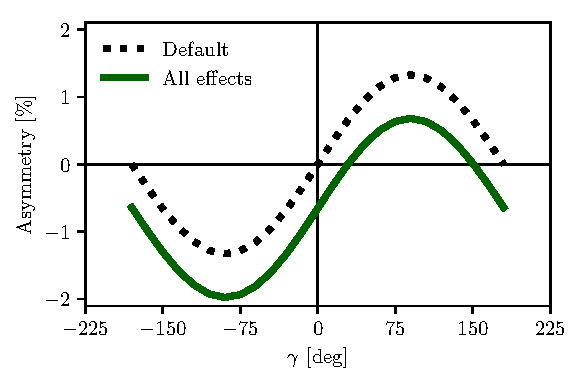
\includegraphics{figures/ks_chapter/paper_asym_for_gammas.pdf}
    \caption{The asymmetry $A_\text{total}$ as a function of $\gamma$ calculated to $O(\epsilon)$ using Eq.~\eqref{eq:global_asym}. The calculation is made for (black dotted line) the default case where $\Delta h = 0$ and (green) including neutral kaon \CP-violation and material interaction with $r_\chi=\epsilon$.}
    \label{fig:global_asym}
\end{figure}

The second observation relates to potential future measurements of $\gamma$, which may also include sensitivity from the total, phase-space-integrated yield asymmetry
\begin{align}\label{eq:global_asym}
    A_\text{total}=\frac{N^--N^+}{N^-+N^+} = 
    \frac{ 2(2\mathcal F_+ -1)r_B \sin \delta_B \sin \gamma +\Delta h}
    {1 + r_B^2+ 2(2\mathcal F_+ -1) r_B \cos \delta_B \cos \gamma} + \mathcal O(r\epsilon),
\end{align}
where the definition of $\mathcal F_+$ from Section~\ref{sub:relation_to_glw_and_ads_measurements} has been employed. In the limit $r_B\to 0$ the expression agrees with the result for the analogous asymmetry in $\Dpm\to\pipm\KS$ decays in Ref.~\cite{grossmanCPViolationKSv2012}, evaluated to $\mathcal O(\epsilon)$ for an infinite and uniform time-acceptance. As hinted at above, the fact that $\mathcal F_+\simeq 0.5$ means that the asymmetry due to $\gamma$ being non-zero is not $\mathcal O(r_B)$, but of approximately the same order of magnitude as the asymmetry due to \CP violation in the neutral kaon sector, governed by $\Delta h$. This is illustrated in Fig.~\ref{fig:global_asym}, where the expression in Eq.~\eqref{eq:global_asym} is plotted in the default case where $\Delta h=0$, as well as including neutral kaon \CP violation and material interaction effects.\footnote{The calculation uses the amplitude model in Ref.~\cite{Belle2018} to calculate \Ki and \ci,  and assumes $r_\chi=\epsilon$, with $\epsilon$ taking the value in Eq.~\eqref{eq:PDG_epsilon}.} The asymmetry changes significantly when including the latter effects. Therefore, measurements based only on the global asymmetry will suffer relative biases of tens of degrees, not a few degrees, if neutral kaon \CP violation and material interaction is not taken into account. 


% subsection impact_on_ (end)

% section detector_descriptions_for_lhcb_and_belle_ii (end)

\section{\texorpdfstring{Impact on BPGGSZ measurements of $\gamma$:\\LHCb and Belle II measurements}{Impact on BPGGSZ measurements of gamma: LHCb and Belle II measurements}} % (fold)
\label{sec:impact_on_ggsz_measurements}

The previous section has established that the bias due to neutral kaon \CP violation and material interaction is at the sub-percent level for measurements based on \BtoDK decays, and just a few percent in \BtoDpi decays. Thus, the effects only contribute a manageable systematic uncertainty in the measurement that is the subject of the thesis. However, the expected precision on $\gamma$ measurements will increase significantly in the coming decade, as both the \lhcb~\cite{lhcbcollaborationPhysicsCaseLHCb2019} and Belle II~\cite{kouBelleIIPhysics2019} collaborations expect to make BPGGSZ measurements that measure \g with a precision of 1--3$^\circ$. Therefore a deeper understanding of the expected bias for these specific experiments is important.

This section details a study, where the equations of the previous section are evaluated numerically to all orders in $\epsilon$, $r_B$, and $r_\chi$, and care is taken to realistically model the experiment-specific conditions. The scope of the original analysis, published in Ref.~\cite{KsCPV}, was a stand-alone paper that covers both \lhcb and Belle~II, and which therefore does not rely on full detector simulation. Instead the following approaches are taken to model the necessary input
\begin{itemize}
  \item the experimental time-acceptance is modelled based on the detector geometry and typical neutral kaon momentum spectrum
  \item the material interaction is included, using the material budget information available in the technical design reports on each experiment
  \item both the time-acceptance and material interaction depends on the neutral kaon momentum, for which realistic distributions are estimated using the \texttt{RapidSim} simulation package~\cite{cowanRapidSimApplicationFast2017}.
\end{itemize}
Each input is described in detail in the following sections. The study has been repeated to assign a systematic uncertainty to the \lhcb measurement in Chapter~\ref{ch:5-GGSZ-measurement}, with slight adjustments to match the exact fit setup and with the inputs above extracted from full \lhcb simulation. This is described further in Section~\ref{sub:the_impact_on_coupled_btodk_and_btodpi_measurements}.

\subsection{Detector geometries} % (fold)
\label{sub:detector_geometries}

The \lhcb geometry and sub detectors are described in details in Chapter~\ref{ch:3-detector}. In the \lhcb measurement discussed in Chapter~\ref{ch:5-GGSZ-measurement}, the \KS mesons are reconstructed in the $\pip\pim$ final state and two distinct categories of decay are considered, depending on where in the detector the \KS decay occurs. The categories have very different decay-time acceptance, and therefore  two scenarios are considered for \lhcb:  one in which the decay products of the \KS leave reconstructed tracks in both the silicon vertex detector and downstream tracking detectors (denoted \emph{long-long} or LL), and one in which the decay products of the \KS only leave tracks in the downstream tracking detectors (denoted \emph{down-down} or DD). 

\begin{figure}[tb]
  \centering
  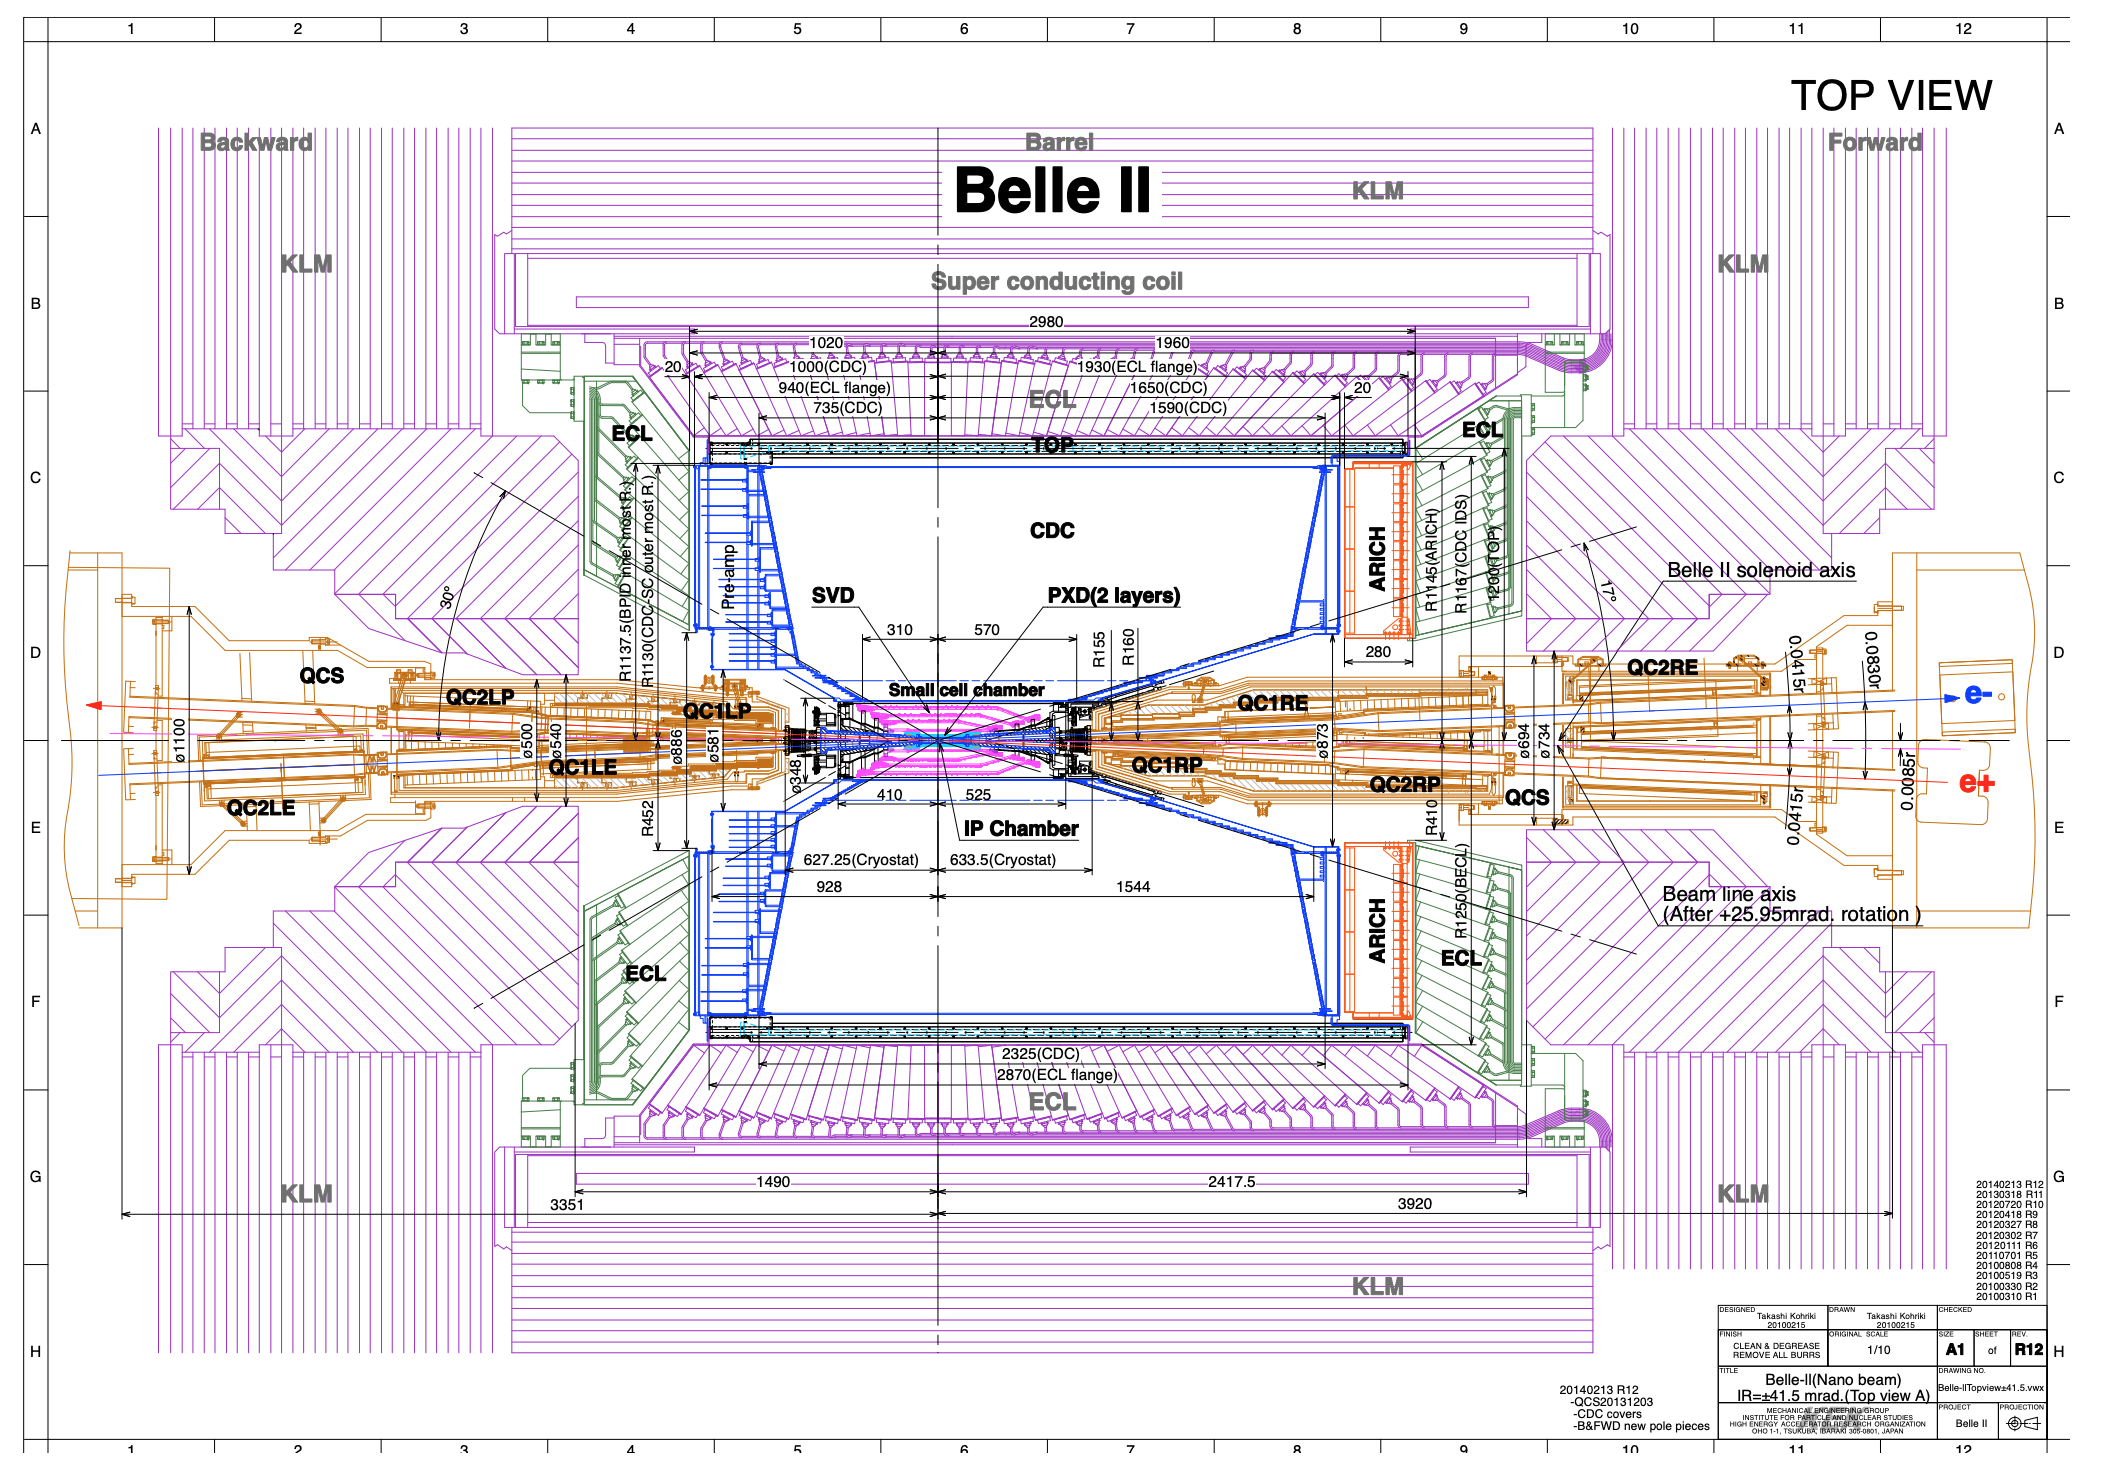
\includegraphics[width=0.95\columnwidth]{figures/ks_chapter/belledetector.png}
  \caption{Schematic of the Belle~II detector, reproduced from Ref.~\cite{kouBelleIIPhysics2019}.}
  \label{fig:belleII_detector}
\end{figure}

The Belle~II detector is a general purpose spectrometer, built to to collect data from asymmetric $e^+e^-$ collisions provided by the SuperKEKB accelerator in Japan~\cite{ohnishiAcceleratorDesignSuperKEKB2013}. A schematic of the detector is shown in Fig.~\ref{fig:belleII_detector}. The relevant sub detectors for the present study are the tracking detectors: a central silicon vertex detector, comprised of a total of six layers within 140\mm of the beam, and a large volume drift chamber with 56 wire layers, extending to a radius of 1130\mm~\cite{kouBelleIIPhysics2019}. 
A single scenario is considered for \belle II, because essentially all the \KS mesons produced in signal decays in Belle II decay within the tracking volume, with more than 90\,\% decaying in the vertex detector according to the studies described below. Thus, three scenarios are considered in total: LL \lhcb, DD \lhcb, and \belle II.

% subsection detector_geometries (end)

\subsection{Kaon momentum distributions} % (fold)
\label{sub:kaon_momentum_distributions}

The neutral kaon momentum distributions are obtained using \texttt{RapidSim}~\cite{cowanRapidSimApplicationFast2017}, a simple tool to generate MC samples. \texttt{RapidSim} has an inbuilt capability to generate decays of \B mesons with the kinematic distribution found in \lhcb collisions and falling in the \lhcb acceptance. However, the distributions need to be reweighted to take the kaon-decay-time acceptance into account. After being reweighted, the \texttt{RapidSim} momentum spectra are reasonably close to those found in samples of $\Bpm\to\D(\to\KS\pip\pim)\Kpm$ decays from full \lhcb simulation, as seen in Fig.~\ref{fig:rapidsim_momentum_comparison}


\begin{figure}[tbp]
    \centering
    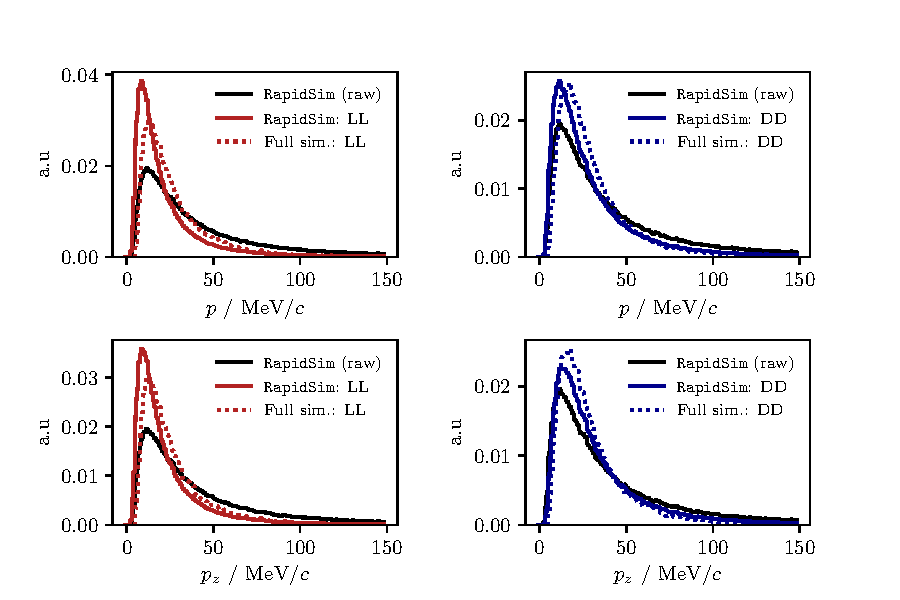
\includegraphics[width=0.98\columnwidth]{figures/analysis/systematics/momentum_distributions_rapidsim_vs_lhcb.pdf}
    \caption{Momentum spectra for the \KS meson in \lhcb, as generated using \texttt{RapidSim} (black lines) directly, as well as reweighed to match decay time acceptance in the (red) LL and (blue) DD data categories of \lhcb. The \lhcb spectra are compared with the spectra in fully simulated signal decays, for both the (dotted red lines) LL and (dotted blue lines) DD data categories.}
    \label{fig:rapidsim_momentum_comparison}
\end{figure}

At \belle II, the signal \B mesons stem from decays of $\Upsilon(4S)$ mesons  produced in asymmetric \text{electron-positron} collisions. This leads to substantially different decay kinematics in comparison to those found at \lhcb. The momentum distribution in \belle II is estimated by letting \texttt{RapidSim} decay \B mesons with a momentum of 1.50 \gevc along the $z$-axis, corresponding to the $\gamma\beta=0.28$ boost of the centre-of-mass system in \belle II when operated at the $\Upsilon(4S)$ resonance~\cite{kouBelleIIPhysics2019}. A perfect $4\pi$ angular acceptance is assumed.   It is not necessary to reweigh the Belle~II momentum spectrum to account for the kaon-decay-time acceptance because all produced \KS mesons decay in the tracking volume. 

The resulting momentum distributions for the three types of sample are shown in Fig.~\ref{fig:momentum}.




\begin{figure}[tbp]
    \centering
    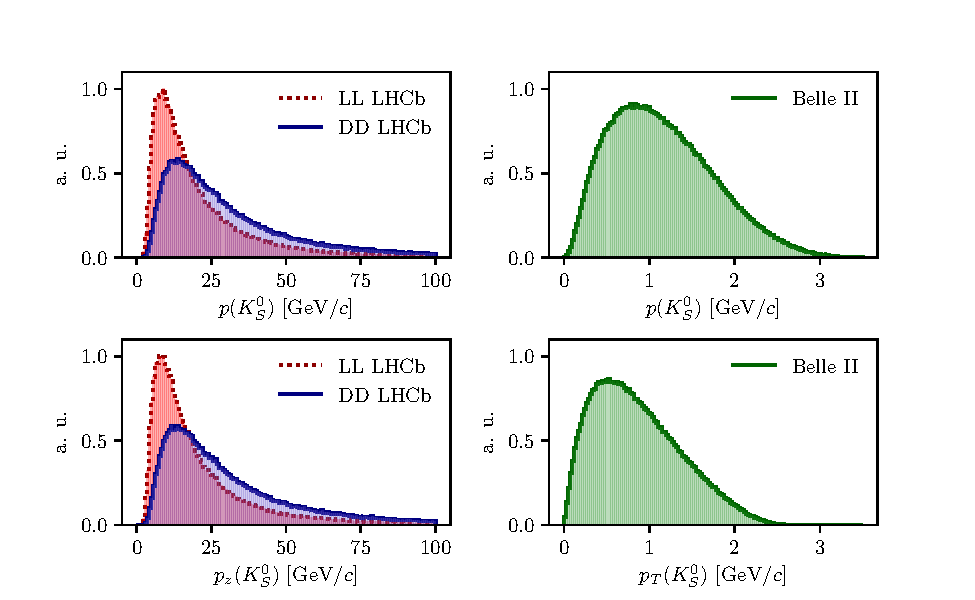
\includegraphics[width=0.98\columnwidth]{figures/ks_chapter/momentum_distributions.pdf}
    \caption{Momentum distributions for the \lhcb (red dotted line) LL and (blue) DD categories, as well as (green) \belle II, obtained using \texttt{RapidSim}.}
    \label{fig:momentum}
\end{figure}


% subsection kaon_momentum_distributions (end)

\subsection{Experimental time acceptance} % (fold)
\label{sub:experimental_time_acceptance}

In order to model the experimental time acceptance, the time-dependent decay rates are only integrated over a finite time interval $(\tau_1, \tau_2)$. The intervals are defined for each of the three experimental categories, by requiring that a neutral kaon, if produced at $x=y=z=0$ with momentum $p=(p_T, p_z)$, decays within the relevant part of the corresponding detector. For the LL \lhcb category, it is required that the kaon decays before reaching $z_{max}=280\mm$, corresponding to a decay where the decay products traverse at least 3 VELO segments (ignoring a number of widely spaced VELO segments placed at a distance of up to $z=750\mm$ from the interaction point)~\cite{CERN-LHCC-2003-030}. For the DD \lhcb category a decay at $z\in[280,2350]\mm$ is required, corresponding to decay between the LL cut-off and the first downstream tracking station~\cite{LHCb-2003-140}. 
%The decay-time distribution using these cutoff values are compared that found in full \lhcb simulation in Fig.~\ref{fig:dec_time_dist}. It is found to be reasonably good, especially in the DD category. In the LL category, the physical cut-off is less well-defined, because the $z$ position of the last VELO tracking segment a given track intersects depend on the angle with the beam line. In the studies used to assign a systematic uncertainty on the \lhcb measurement in Chapter~\ref{ch:5-GGSZ-measurement}, a better acceptance model was employed, defined with a soft turn-on based on full \lhcb simulation. The expected decay-time distribution assuming this acceptance function is also shown in Fig.~\ref{fig:dec_time_dist}.
The time acceptance has a significant impact for the \lhcb categories, where some 20\,\% of the kaons escape the tracking stations completely before decaying.

% \begin{figure}[tb]
%     \centering
%     \begin{subfigure}{\columnwidth}\centering
%         \includegraphics[width=0.8\columnwidth]{figures/ks_chapter/note_figs/lhcb_studies/1d_DD_time_acceptance_result.pdf}
%         \caption{}\label{fig:dec_time_dist_DD}
%     \end{subfigure}
%     \begin{subfigure}{\columnwidth}\centering
%         \includegraphics[width=0.8\columnwidth]{figures/ks_chapter/note_figs/lhcb_studies/1d_LL_time_acceptance_result.pdf}
%         \caption{}\label{fig:dec_time_dist_LL}
%     \end{subfigure}
%     \caption{Decay time distribution of simulated \lhcb signal decays in the (top) DD and (bottom) LL data categories, for four different, narrow $p_z(\KS)$ regions. The expected distributions given the time acceptance used in the simple studies  are overlaid.\label{fig:dec_time_dist}} 
% \end{figure}

For \belle II, it is assumed that the \KS reconstruction is similar to {}the \belle\ \KS reconstruction, which is based on a neural network and reconstructs \KS decays for which the decay product leave tracks in both the drift chamber and silicon vertex detectors, as well as decays that leave tracks in the drift chamber only~\cite{BelleKSPaper,BelleKSThesis}. Therefore, the \KS decay is required to be within $r_{max}=1130\mm$ of the beam axis, corresponding to a decay within the outer radius of the drift-chamber. In practice, most of the kaons already decay inside the silicon vertex detector, and requiring a decay before the outer radius of the drift chamber is essentially equivalent to having no time cut-off.



% subsection experimental_time_acceptance (end)

\subsection{Detector material budget} % (fold)
\label{sub:detector_material_budget}

The effect of the material interaction is governed by parameter $\Delta\chi$ of Eq.~\eqref{eq:mat_param}. The parameter varies along a given kaon path, as the kaon intersects detector components made of different materials. In these studies, the calculations are simplified by using a single average material parameter for each experimental scenario. The average material parameters can be estimated for a given experimental scenario by considering the type and length of material traversed by a kaon in the relevant sub-detector(s). The average value is estimated, by exploiting that $\Delta\chi$ is related to the forward scattering amplitude $f$ $(\bar f)$ of \Kz (\Kzb) mesons in a given material~\cite{goodRelationScatteringAbsorption1957,fetscherRegenerationArbitraryCoherent1996}
\begin{align}\label{eq:mat_delta_chi}
    \Delta \chi = - \frac{2\pi \mathcal{N}}{m_K}(f-\bar f) = - \frac{2\pi (N_A \rho/A)}{m_K}(f-\bar f),
\end{align}
where $\mathcal{N}=N_A\rho/A$ is the scattering centre density of the material, $m_K$ is the mass of the kaon state,  $A$ and $\rho$ are the nucleon number and density of the material, and $N_A$ is Avogadro's number.
Measurements made for a range of nuclei~\cite{Gsponer1979} show that in the momentum range $p_K\in [20, 140]\gevc$
\begin{align} \label{eq:f_p_dep}
    \left|\frac{f-\bar f}{p_K}\right| = 2.23 \frac{A^{0.758}} {p_K^{0.614} (\gevc)} \text{ mb}, \quad \arg [f - \bar f] = -\frac{\pi}{2}\left(2-0.614\right),
\end{align}
where the phase of $\Delta f$ is determined via a phase-power relation~\cite{Briere1995}. In the numerical studies presented here, Eq.~\eqref{eq:f_p_dep} is also used for the low momentum neutral kaons in the \belle II calculations, as a more detailed modelling of the low momentum $\Delta\chi$ based on Ref.~\cite{Ko2011} is found to yield very similar results. The scattering centre density $\mathcal{N}$ is approximated as being constant, equal to the average density along a neutral kaon path due to its intersection with different detector segments. This average is estimated using the simplifying assumption that the total detector material budget is due to silicon. In practice, $\mathcal{N}=N_A\rho/A$ is calculated using $A=28$ and $\rho = f^\text{Si}\rho^\text{Si}$, where $f^\text{Si}<1$ is the average fraction of a neutral kaon path length that is inside detector material, estimated via the known dimensions of the detector, the average nuclear interaction length seen by a track traversing it cf. the technical design reports~\cite{CERN-LHCC-2003-030,RICH-TDR}, and the nuclear interaction length of silicon $\lambda_I^\text{Si}=465.2\mm$~\cite{PDG2020}. 
The average value of $r_\chi=\frac{1}{2}\frac{\Delta\chi}{\Delta\lambda}$, which governs the size of the matter regeneration effect, can be calculated for the three considered experimental scenarios and satisfy $|r_\chi^\text{LL}|=2.7\times10^{-3}$, $|r_\chi^\text{DD}|=2.2\times10^{-3}$, and ${|r_\chi^\text{Belle II}|=1.0\times10^{-3}}$. 

The neutral kaon tracks in \lhcb generally pass through somewhere between zero (for a significant amount of the LL tracks) and a hundred (for some DD tracks) distinct detector segments. Therefore it is worth examining the degree to which using a single average $\Delta\chi$ value, obtained following the procedure outlined above, provides a reasonable description of the average material interaction. This can be done using full \lhcb simulation, where the kaon state for a simulated track can be evaluated at all times, by applying Eq.~\eqref{eq:mat_time_dep} iteratively for each detector segment the track traverses, using a $\Delta\chi$ value appropriate for that segment. 
%The results can then be compared to those obtained using a single average $\Delta\chi$. 
This is done in Fig.~\ref{fig:lhcb_asymmetry} for a simple observable: the yield asymmetry 
\begin{align}\label{eq:KKb_asymmetry_definition}
    A_{K^0} = \frac{|\psi_{\Kz}(t)|^2 - |\psi_\Kzb(t)|^2}{|\psi_{\Kz}(t)|^2 + |\psi_\Kzb(t)|^2},
\end{align}
where $\psi_{\Kz}(t)$ ($\psi_\Kzb(t)$) is the amplitude for an initial \Kz (\Kzb) to decay to two pions at time $t$. In this calculation, it is assumed that $\epsilon=0$ to isolate the material effect with no asymmetry contribution from the inherent \CP-violation in the neutral kaon sector. While the track-by-track asymmetries are found to differ significantly depending on the exact detector segments a track intersects, the average asymmetry is seen to evolve smoothly as a function of decay time, and in reasonable agreement with the asymmetry value that is calculated using the average $\Delta\chi$ values estimated above. 


\begin{figure}[tb]
    \centering
    \includegraphics[width=\columnwidth]{figures/analysis/systematics/compare_material_int_asym.pdf}
    \caption{The asymmetry in Eq.~\eqref{eq:KKb_asymmetry_definition} as a function of time for \KS tracks in samples of simulated (left) LL and (right) DD decays, using the full \lhcb simulation. The light blue area is the central 50 \% quantile of all tracks, the dark blue area is the 1$\sigma$ uncertainty band on the mean. The black lines show the result for a subset of individual, randomly sampled tracks. The red lines are calculated using the average $\Delta\chi$ values that are also used in the calculation of biases in BPGGSZ measurements.}
    \label{fig:lhcb_asymmetry}
\end{figure}



The \lhcb detector is undergoing a significant upgrade prior to the start of the LHC Run~3. However, the material budget and geometry of the relevant sub-detectors will be similar to the sub-detectors used during Run~1~and~2~\cite{VELOUpgradeTDR,PIDUpgradeTDR}. Hence the results of this study will be valid for measurements during the upgrade phases of \lhcb, even though the detector parameters presented in this section relate to the original \lhcb detector.

% subsection detector_material_budget (end)

\subsection{Calculation procedure} % (fold)
\label{sub:calculation_procedure}

The main idea in the bias study is to calculate the BPGGSZ bin yields including the full effect of neutral kaon \CP violation and material, fit them using the default equations of Chapter~\ref{ch:2-litreview}, and thereby obtain the bias $\Delta\gamma = \gamma - \gamma^0$ due to the kaon effects not being considered in the parameter extraction. For the purpose of Ref.~\cite{KsCPV}, a simple fit setup of a single \BtoDh mode is investigated, where the \Ki parameters are determined in a control channel with the relevant experimental acceptance. This setup is modified in the study used to assign a systematic uncertainty on the \lhcb measurement of Chapter~\ref{ch:5-GGSZ-measurement}, as described in Section~\ref{sub:the_impact_on_coupled_btodk_and_btodpi_measurements} below.


In practice, the amplitude model for $\Dz\to\KS\pip\pim$ decays in Ref.~\cite{Belle2018} is taken to represent the $A_1(\spm)$ amplitude. Then $A_2(\spm)$ is obtained as described in Section~\ref{sub:relationship_between_the_ks_and_kl_amplitudes}. In terms of $A_1$ and $A_2$, the amplitudes $\ADorDbSL(\spm)$ can be expressed and related via Eqs.~\eqref{eq:A12toKS}~and~\eqref{eq:DDbar_relations}, and the full signal decay amplitudes as a function of phase-space coordinates, time, and the material interaction parameter $\Delta\chi$ can be calculated for a given set of input parameters $(\gamma^0, r_B^0, \delta_B^0)$. The squared decay amplitudes are then integrated over phase space and the kaon decay times to obtained the binned signal yield.

The signal yields depend on the momentum via the time-acceptance parameters $\tau_1$ and $\tau_2$, and because the material interaction parameter $\Delta\chi$ is momentum dependent. Therefore, the yields are averaged over the \KS momentum distributions of \lhcb and \belle II. 


The parameters \xpm and \ypm are determined by a maximum likelihood fit to the calculated yields, after which the fit result and covariance matrix are interpreted in terms of the physics parameters $(\gamma, r_B, \delta_B)$ using another maximum likelihood fit~\cite{LHCb-PAPER-2016-032}. In the fits, the $K_i$ are obtained using the definition $K_i=K_i^\text{meas}=({N^\D_i + N^\Dbar_{-i}})/({\sum_j N^\D_j +N^\Dbar_{-j}})$, in terms of the expected yields $N^\D_i$ ($N^{\Dbar}_i$) of a flavour-tagged \Dz (\Dzb) decays in bin $i$ of the \D decay phase space, calculated as described above for $r_B^0=0$. This corresponds to experimentally measuring the $K_i$ in a control channel, and takes the effect of neutral kaon \CP violation and material interaction on $K_i$ measurements into account, as well the experimental time acceptance. The $(c_i, s_i)$ are calculated using $A_1(\spm)$ and the experimental time acceptance is taken into account in this calculation as well. 



% subsection calculation_procedure (end)




 











\subsection{Results} % (fold)
\label{sub:bias_results}


\begin{figure}[tbp]
    \centering
    \includegraphics{figures/ks_chapter/gamma_scan_Belle2018_50_g.pdf}
    \caption{The bias $\Delta \gamma$ as a function of input $\gamma_0$ for (left) the LL \lhcb category, (centre) the DD \lhcb category, and (right) \belle II. The bias is calculated due to (blue, dashed line) neutral kaon \CP violation alone, (red, dotted line) material interaction alone, and (green line) both effects. The shaded region shows the estimated $1\sigma$ uncertainty band.}
    \label{fig:compare_experiments}
\end{figure}


The obtained bias $\Delta\gamma$ is shown as a function of input $\gamma^0$ for the various experimental conditions in Fig.~\ref{fig:compare_experiments}. The calculations are made using $(r_B^0, \delta_B^0)=(0.1, 130^\circ)$, approximately equal to the physics parameters relevant for $\Bpm\to\D\Kpm$ decays~\cite{UTfit-UT,HFLAV}.  The bias does not vary significantly with $\gamma^0$ in the plotted range, which includes the world average value of direct $\gamma$ measurements as well as the values obtained in full unitarity-triangle fits~\cite{HFLAV,UTfit-UT,CKMfitter2015}. For all cases, the bias is found to be below $0.5^\circ$, corresponding to relative biases of about half a percent. Thus the biases are of $\mathcal O(r\epsilon /r_B)$ as expected, given the arguments of Section~\ref{sub:modification_of_the_bpggsz_yield_equations}. The contributions from the individual \KS CPV and material interaction effects are also shown. It is seen that the neutral kaon \CP violation and material interaction effects leads to approximately equal biases in all three cases. 

Given the decay-time acceptance and momentum distribution for each experimental category, the mean life time, $\langle\tau\rangle$, of the reconstructed kaons can be calculated. In terms of the \KS lifetime ${\tau_\KS=(0.895\pm0.004)\times10^{-11}\,}$s~\cite{PDG2020}, $\langle\tau_\text{LL}\rangle\simeq0.1\tau_\KS$ for the \lhcb LL category, $\langle\tau_\text{DD}\rangle\simeq0.8\tau_\KS$ for the \lhcb DD category, and at \belle II $\langle\tau_\text{Belle II}\rangle\simeq\tau_\KS$. The difference in average kaon lifetime is reflected in the observed biases, which are found to be larger in the samples with longer lived kaons. The very small effect in the LL category is to be expected because the \CP-violation effect due to \KS not being \CP-even is approximately cancelled by the \CP-violation effect arising from $\KS-\KL$ interference for kaons with decay times much smaller than $\tau_\KS$~\cite{grossmanCPViolationKSv2012}. 
%The time dependence of the bias effect means that it can potentially be beneficial to restrict a measurement to using short-lived \KS mesons in a future scenario, where the impact of \KS\ \CP violation is comparable to the statistical precision of the measurement. For example, the bias can reduced by 40\,\% in the \belle II scenario if only \KS mesons decaying within 8\cm of the beam axis are included in the measurement. This requirement only removes 20\,\% of the signal yield, and hence only increases the statistical uncertainty of the measurement by 10\,\%.

The uncertainty bands in Fig.~\ref{fig:compare_experiments} are calculated by repeating the study while varying some of the inputs. The model dependence of the predicted biases is probed by repeating the study using two other amplitude models as input for $A_1(\spm)$ and $A_2(\spm)$: the model published in Ref.~\cite{BELLE2010} and the model included in \sc{EvtGen}\normalfont~\cite{EvtGen}. 
%The use of different models change the predicted biases by up to $0.05^\circ$. W
When defining $A_2(\spm)$ in terms of $A_1(\spm)$, there is an uncertainty due to the unknown $(r_k, \delta_k)$ parameters used to describe the $\pi\pi$ resonance terms. This uncertainty is assessed by making the study with several different random realisations of the parameter set. 
%The phases $\delta_k$ are sampled uniformly in the interval $[0, 2\pi]$ while the $r_k$ are sampled from a normal distribution with $\mu=\tan^2\theta_C$ and $\sigma=\mu/2$. The uncertainty is about $0.05^\circ$ across the three experiments considered. 
The studies are repeated while varying the time acceptances and material densities with $\pm 10\,\%$. 
%The largest deviations in biases are found to be below $0.05^\circ$. The dependence on the handling of the momentum distribution is estimated by repeating the study using 10 and 20 quantiles to describe the momentum distributions at each point in phase space, instead of 5. The variation in the results is taken as the systematic uncertainty, and found to be below $0.01^\circ$ for all experiments. 
There is an additional uncertainty due to the use of simulation samples generated with \texttt{RapidSim} to describe the kaon momentum distribution, in lieu of full detector simulations. 

There is also an uncertainty from the use of $(\ci, \si)$ as calculated using $A_1(\spm)$. It is to be expected that the measured values $(\hat c_i, \hat s_i)$ from the \cleo collaboration differ by those calculated using $A_1^D(s_-,s_+)$ by terms of $\mathcal O(\epsilon)$ due to neutral kaon \CP violation, which is not taken into account in the measurement~\cite{CLEOCISI}. These corrections can be calculated via a procedure analogous to the one used to estimate the corrections on measurements of $\gamma$ in this paper. However, as these corrections are much smaller than the experimental uncertainties in the measurement, they have not been studied further.

%It is interesting to evaluate the bias obtained if the \Ki are calculated from $A_1(\spm)$, without any corrections due to neutral kaon \CP violation and material interaction. If this is done, while the full experimental time acceptance is taken into account, the biases only change by up to $0.01^\circ$, across the experiments. This is because the $O(\epsilon)$ corrections in Eq.~\eqref{eq:hat_Ki}, where the expected measured \Ki is given to lowest order in $\epsilon$ and $r_\chi$, only affect the overall normalisation. If the time acceptance \emph{is not} taken into account, biases of several degrees can occur, irrespective of the presence of neutral kaon \CP violation or material interaction effects. 


\begin{figure}[tbp]
    \centering
    \includegraphics{figures/ks_chapter/delta_scan_Belle2018_50_g.pdf}
    \caption{The bias $\Delta \gamma$ as a function of input $\delta_B$ for (left) the LL \lhcb category, (centre) the DD \lhcb category, and (right) \belle II. The bias is calculated for $\gamma=75^\circ$ and (green line) $r_B=0.005$, (blue, dashed line) $r_B=0.1$, and (red, dotted line) $r_B=0.25$. The shaded region shows the estimated $1\sigma$ uncertainty band.}
    \label{fig:delta_scan}
\end{figure}


For the purpose of this thesis, it is important to consider the bias in measurements that use \BtoDpi decays as well, and other \B decay modes can also be used in BPGGSZ measurements, such as $\Bpm\to\Dstar\Kpm$, $\Bpm\to\D\Kstarpm$, and $\Bz\to\D\Kstarz$. For the purpose of the study presented here, the main difference between the decay channels is that they have different values of $r_B$ and $\delta_B$. Figure~\ref{fig:delta_scan} shows $\Delta\gamma$ as a function of input $\delta_B^0$, for $\gamma^0=75^\circ$ and three different values of $r_B^0$. Aside from $r_B^0=0.1$, the results are shown for $r_B^0=0.005$, which corresponds to the expectation in $\Bpm\to\D\pipm$ decays~\cite{rDpi} and $r_B^0=0.25$, which corresponds to $\Bz\to\D\Kstarz$ decays~\cite{LHCb-CONF-2018-002}. The most notable feature is that the biases are significantly larger in the \BtoDpi case. This is expected: the $r^0_B$ dependent behaviour is governed by the relative importance of different $\mathcal O(r\epsilon)$ correction terms to the phase-space distribution. There are terms of both $\mathcal O(r_A\epsilon)$ and $\mathcal O(r_B\epsilon)$\footnote{There are similar terms of $\mathcal O(r_Ar_\chi)$ and $\mathcal O(r_Br_\chi)$, but as $\epsilon$ and $r_\chi$ are of the same order of magnitude, these terms can be treated completely analogously to the $\mathcal O(r_A\epsilon)$ and $\mathcal O(r_B\epsilon)$ terms, and have been left out of the discussion for brevity.}, which lead to expected biases of size $\mathcal O(r_A\epsilon/r_B)$ and $\mathcal O(r_B\epsilon/r_B)=\mathcal O(\epsilon)$, respectively, cf. the discussion of Section~\ref{sub:modification_of_the_bpggsz_yield_equations}. 
In the $\Bpm\to\D\pipm$ case, the $\mathcal O(r_A\epsilon)$ correction terms dominate because $r_A/r_B\simeq (0.05/0.005)=10$. This explains the relatively large bias, as $|r_A\epsilon/r_B^{D\pi}|\simeq 4\%$. The bias is seen to be up to {}$\pm1.5^\circ$, but only about $+0.2^\circ$ with the expected value of $\delta_B^{D\pi}\simeq300^\circ$~\cite{LHCb-PAPER-2016-032,rDpi}. These biases are \emph{much smaller} than the precision on $\gamma$ that is obtainable in a \BtoDpi analysis with current experimental yields, and do thus not pose a problem.
In the $r_B^0=0.1$ and $r_B^0=0.25$ cases the $\mathcal O(r_B\epsilon)$ correction terms dominate, and the biases are of $O(\epsilon)$, independent of the $r_B^0$ value. Therefore both cases have biases of similar size.



Further, it is clear that the biases depend on $\delta_B^0$ and that the oscillation period of the $\delta_B$ dependence is different between the $r^0_B=0.005$ case and the $r_B^0\in\{0.1, 0.25\}$ cases. It is to be expected that $\Delta\gamma$ oscillates as a function of $\delta^0_B$, because $\delta_B^0$ enters the yield equations via $\cos(\delta_B^0\pm\gamma)$ and $\sin(\delta_B^0\pm\gamma)$ terms.  As explained above, the $\mathcal O(r_A\epsilon)$ terms dominate the \BtoDpi bias, and these are independent of $\delta_B^0$. The $\mathcal O(r_B\epsilon)$ terms, however, are important for the bias corrections for larger $r_B$ values, and the terms include factors of $\cos(\delta_B^0\pm\gamma)$ and $\sin(\delta_B^0\pm\gamma)$. This explains the different bias dependence on $\delta^0_B$. 


While the input value of $\gamma^0=75^\circ$ was chosen for these studies, there is minimal variation in the results if another value of $\gamma^0$ in the range $[60^\circ, 85^\circ]$ is used.


\subsection{\texorpdfstring{Coupled \BtoDK and \BtoDpi measurements}
{Coupled B->DK and B->Dpi measurements}}% (fold)
\label{sub:the_impact_on_coupled_btodk_and_btodpi_measurements}

The studies presented above have been extended on two accounts in order to assign a systematic uncertainty to the \lhcb measurement presented in Chapter~\ref{ch:5-GGSZ-measurement}. Firstly, full \lhcb simulation has been used to obtain the momentum distributions, as well as to fit a better description of the decay-time acceptance and the reconstruction efficiency profile over the \D-decay phase space. Secondly, the fit setup is modified to correspond to the experimental approach described in Section~\ref{sec:strategy_for_lhcb_measurement} and Chapter~\ref{ch:5-GGSZ-measurement}: the signal yields are calculated for both the \BtoDK and \BtoDpi channels, and fitted in a combined fit to obtain $(\xpmdk, \ypmdk, \xxidpi, \yxidpi)$, where the \Fi parameters are allowed to float in the fit. The biases obtained for each observable are shown in Fig.~\ref{fig:LHCb_related_biases}, evaluated using the time-acceptance, momentum distribution, and material budget relevant for the DD category (since the effect in the LL category is much smaller). As will be clear in Chapter~\ref{ch:5-GGSZ-measurement}, these biases are all significantly smaller than the corresponding statistical uncertainties. Thus, the effects of neutral kaon \CP violation and material interactions contribute a manageable systematic uncertainty in current BPGGSZ measurements, even if the \BtoDpi channel is promoted to a signal channel.

\begin{figure}[tb]
  \centering
  \includegraphics[width=0.45\columnwidth]{figures/ks_chapter/delta_xy_dk.pdf}
  \includegraphics[width=0.45\columnwidth]{figures/ks_chapter/delta_xy_dpi.pdf}
  \caption{The bias on (left) the \BtoDK and (right) $\BtoDpi \;\CP$-violation observables in the \lhcb DD category, evaluated in bias studies with inputs based on full \lhcb simulation, calculated as a function of input $\gamma_0$. \mccorrect{Since the typical size of the $x_\pm^{DK}$ and $y_\pm^{DK}$ parameters is $~\sim0.1$, the relative biases on the observables are approximately $0.5\,\%$. Thus, the results are similar to the ones shown in} Fig.~\ref{fig:compare_experiments}.}
  \label{fig:LHCb_related_biases}
\end{figure}

As the statistical uncertainty becomes comparable with the bias effects described in this chapter, the systematic uncertainty should be assigned by a more accurate study, incorporating the traversed material on a track-by-track basis in full detector simulation. Such a detailed calculations can also be used to apply a bias correction if desired. 

% subsection the_impact_on_coupled_btodk_and_btodpi_measurements (end)

\section{Concluding remarks} % (fold)
\label{sec:concluding_remarks}

% subsection concluding_remarks (end)


The analysis presented in this chapter has shown the expected impact of neutral kaon \CP violation and material interaction on current BPGGSZ measurements to be small compared to the statistical uncertainties; first by simple order-of-magnitude estimates and then by a detailed calculation of the expected effect in \lhcb and Belle~II.



While the calculations were made for the case of \DtoKspipi decays, the BPGGSZ approach can of course also be applied in other \D-decay final states, such as ${\D\to\KS\Kp\Km}$ and $\D\to\KS\pip\pim\piz$. The biases on measurements of $\gamma$ based the \D decay phase-space distributions should be of similar size in these decay channels. The impact on $\gamma$ measurements based on the phase-space-integrated yield asymmetry can be expected to be tens of degrees for the $\D\to\KS\Kp\Km$ channel, where the yield asymmetry is expected to be around 2\,\%, for the reasons explained in Section~\ref{sub:modification_of_the_bpggsz_yield_equations}. The $\D\to\KS\pip\pim\piz$ decay, however, is dominantly \CP-odd~\cite{CLEOKSpipipi0}, and the bias in measurements based on the total asymmetry is therefore expected to be $\mathcal O(\epsilon/r_B)$, i.e. a few degrees~\cite{grossmanEffectsBarMixing2014}. More precise calculations of the biases would require a repeat of the study included here, with relevant amplitude models and binning schemes in place.



The chapter focuses on the model-independent, binned approach that is the subject of the thesis. However, the underlying mechanism that determines the scale of the bias, namely that the phase-space \emph{distribution} of signal decays is unaffected at $\mathcal O(\epsilon)$ and $\mathcal O(r_\chi)$, is independent on the exact measurement approach. Therefore it is expected that amplitude-model-based measurements and measurements made with new unbinned methods such as those in Ref~\cite{poluektovUnbinnedModelindependentMeasurements2018} will be similarly biased if kaon \CP violation and regeneration are not accounted for. 
% section impact_on_ggsz_measurements (end)

% section cp_violation_and_material_interaction_of_neutral_kaons (end)



% \begin{savequote}[8cm]
% Alles Gescheite ist schon gedacht worden.\\
% Man muss nur versuchen, es noch einmal zu denken.

% All intelligent thoughts have already been thought;\\
% what is necessary is only to try to think them again.
%   \qauthor{--- Johann Wolfgang von Goethe \cite{von_goethe_wilhelm_1829}}
% \end{savequote}

\chapter{\texorpdfstring{A GGSZ measurement with $\Bpm\to\D h^\pm$ decays}{A GGSZ measurement with B->Dh decays}}
\label{ch:5-GGSZ-measurement}

% \minitoc

First I will return to describing the overall strategy a bit, then one can proceed with the data analysis section

\section{Candidate selection} % (fold)
\label{sec:candidate_selection}

% section candidate_selection (end)

\section{Signal and background components} % (fold)
\label{sec:signal_and_background_components}

% section signal_and_background_components (end)

\section{Measurement of the CP-violation observables} % (fold)
\label{sec:measurement_of_the_cp_violation_observables}

% section measurement_of_the_cp_violation_observables (end)

\section{Systematic uncertainties} % (fold)
\label{sec:systematic_uncertainties}

% section systematic_uncertainties (end)

\section{\texorpdfstring{Obtained constraints on $\gamma$}{Obtained constraints on gamma}} % (fold)
\label{sec:constraints_on_gamma}

% section constraints_on_ (end)

% section cp_violation_and_material_interaction_of_neutral_kaons (end)



% \begin{savequote}[8cm]
% Alles Gescheite ist schon gedacht worden.\\
% Man muss nur versuchen, es noch einmal zu denken.

% All intelligent thoughts have already been thought;\\
% what is necessary is only to try to think them again.
%   \qauthor{--- Johann Wolfgang von Goethe \cite{von_goethe_wilhelm_1829}}
% \end{savequote}

\chapter{Summary and outlook}
\label{ch:6-conclusion}

The main result of the thesis is a measurement of the CKM angle $\gamma$ using \BtoDK and \BtoDpi decays, where \D denotes a superposition of the \Dz and \Dzb states that decays to one of the final states \Kspipi and \KsKK. Approximately 17,500 \BtoDK decays\footnote{This number includes the approximately 13.5\,\% of \BtoDK that are reconstructed as \BtoDpi decays in the analysis.} and 230,000 \BtoDpi decays are analysed, obtained from the $pp$ collision data set collected by the \lhcb experiment during Run~1~and~2 of the LHC. The total data set corresponds to an integrated luminosity of about 8.7\invfb collected at centre-of-mass energies of $\sqrt s =7$, $8$, and $13\tev$. The measurement relies on the phase-space distribution of signal decays, analysed using a model-independent method based on strong-phase measurements by the CLEO and BESIII collaborations; an approach known as the model-independent BPGGSZ method. The measured \CP-violation observables are defined
\begin{align}
    \xpmdk &= r_B^{DK} \cos (\delta_B^{DK} \pm \g), & \ypmdk &= r_B^{DK} \sin (\delta_B^{DK} \pm \g),
\end{align}
and measured to be
\begin{align}
\begin{split}
    x_-^{DK} & = (\phantom{-}5.68 \pm 0.96 \pm  0.20\pm 0.23) \times 10^{-2}, \\
    y_-^{DK} & = (\phantom{-}6.55 \pm 1.14 \pm  0.25\pm 0.35) \times 10^{-2}, \\
    x_+^{DK} & = (         - 9.30 \pm 0.98 \pm  0.24\pm 0.18) \times 10^{-2}, \\
    y_+^{DK} & = (         - 1.25 \pm 1.23 \pm  0.26\pm 0.28) \times 10^{-2},
\end{split}
\end{align}
where the first uncertainty is statistical, the second arises due to systematic effects in the measurement, and the third is the propagated uncertainty on the strong-phase inputs from the CLEO and BESIII measurements. In addition, two nuissance parameters relating to \BtoDpi decays are measured. These are defined
\begin{align}
    \xxidpi &= (r_B^{DK}/r_B^{D\pi}) \cos (\delta_B^{DK} - \delta_B^{D\pi}), & 
    \yxidpi &= (r_B^{DK}/r_B^{D\pi}) \sin (\delta_B^{DK} - \delta_B^{D\pi}),
\end{align}
and measured to be
\begin{align}
\begin{split}
    x_\xi^{D\pi} & = (         - 5.47 \pm 1.99 \pm  0.32\pm 0.14) \times 10^{-2}, \\
    y_\xi^{D\pi} & = (\phantom{-}0.71 \pm 2.33 \pm  0.54\pm 0.18) \times 10^{-2}. 
\end{split}
\end{align}
Due to the measurement approach, the information on $\gamma$ obtained from \BtoDpi decays is encoded in the $(\xpmdk, \ypmdk)$ parameters. The measured observables have been interpreted in terms of the underlying physics parameters, yielding the results
\begin{align}
\begin{split}\label{eq:phys_results}
    \gamma          &= (68.7^{+5.2}_{-5.1})^\circ, \\
    r_B^{DK}       &= 0.0904^{+0.0077}_{-0.0075}, \\
    \delta_B^{DK}  &= (118.3^{+5.5}_{-5.6})^\circ, \\
    r_B^{\D\pi}      &= 0.0050^{+0.0017}_{-0.0017}, \\
    \delta_B^{\D\pi} &= (291^{+24}_{-26})^\circ.
\end{split}
\end{align}
This is the most precise stand-alone measurement of $\gamma$ to date, with a precision comparable to that of all earlier measurements of $\gamma$ combined. The measured value agrees with the expectation from global fits of all CKM parameters. For example, the CKMFitter group obtains  $\gamma = (65.66^{+0.90}_{-2.65})^\circ $~\cite{CKMfitter2015} in a global fit that excludes direct $\gamma$ measurements, and the obtained values and uncertainties in other world averages are similar~\cite{HFLAV,UTfit-UT}.

The thesis presented the first  BPGGSZ measurement by the \lhcb collaboration to include \BtoDpi decays as a signal channel, and a series of feasibility studies that informed the analysis strategy has also been presented. While the impact on the $\gamma$ precision from \BtoDpi decays is limited, the new strategy significantly simplified the treatment of the non-uniform phase-space acceptance in \lhcb, and lead to a significant reduction of the systematic measurement uncertainty. This will become especially important in future measurements, where the precision will no longer be limited by the statistical uncertainty to the degree that it is now.

The thesis also presented a careful analysis of the impact of neutral kaon \CP violation and material interaction on $\gamma$ measurements based on the BPGGSZ method. This was a crucial step towards to the promotion of the \BtoDpi channel to a signal channel: existing literature estimated the potential bias to be $\mathcal O(1^\circ)$ in \BtoDK decays \emph{and to scale with} $1/r_B$. This suggested potentially large biases for a \BtoDpi analysis, since $r_B^{D\pi}\simeq0.005$ is twenty times smaller than $r_B^{DK}\simeq 0.1$. However, the thesis argues that the actual impact is an order of magnitude smaller, as long as the determination of the \CP-violation observables is based on the phase-space distribution of signal decays. This is demonstrated in a number of numerical studies that take the detector geometries of the \lhcb and Belle~II detectors into account; these studies are also used to assign a (reasonably small) systematic uncertainty on the measurement results discussed above.

\section{A look towards the future} % (fold)
\label{sec:a_look_towards_the_future}

% section a_look_towards_the_future (end)
% \minitoc

Precise measurements of $\gamma$ play an important role in the physics programmes of both the \lhcb and \belle~II experiments, and the next 10--15 years will see huge improvements in the obtainable precision. Given the results of Chapter~\ref{ch:5-GGSZ-measurement}, it is clear that \lhcb is well on course to reach, even surpass, the expected goal of determining $\gamma$ with a precision of $4^\circ$ using Run~1~and~2 data~\cite{LHCbUpgradeITDR}, when more analyses are performed with the full data set. In the longer run, \lhcb is expecting to reach a precision of $1^\circ$ in the combination of $\gamma$ measurements by the end of Run~4 of the LHC, and on improving that to $\sim 0.35^\circ$ in the planned (but not-yet approved or funded) Upgrade Phase II during the 2030'ies~\cite{lhcbcollaborationPhysicsCaseLHCb2019}, with the BPGGSZ mode continuing to be an important contributor the the obtainable precision. The mode plays an even more significant role in the Belle~II physics programme, being denoted the \emph{golden mode} in the physics programme~\cite{kouBelleIIPhysics2019}, due to a much higher \KS reconstruction efficiency in the experiment. When the planned data set corresponding to an integrated luminosity of 50\invab has been collected, the uncertainty on $\gamma$ from the combination of all Belle~II results is expected to be about $1.6^\circ$~\cite{kouBelleIIPhysics2019}; this is expected to happen in 2031 given the current schedule~\cite{BelleTimescale}.

The main reason for the impressive expected improvement in precision is that current $\gamma$ measurements are dominated by statistical uncertainties in all the major signal modes. This is expected to remain true for the BPGGSZ modes throughout the period described above. The current dominating systematic uncertainty on $\gamma$ is due to the uncertainty on the measured strong-phase inputs, currently contributing an uncertainty of about $\sim1^\circ$; a number that represents a significant improvement compared to earlier analyses, due to the recently published measurements by the BESIII collaboration~\cite{BESCISI,BESCISIKSKK}. These measurements are based on a data set corresponding to an integrated luminosity of 2.9\invfb. The BESIII collaboration is planning to take data corresponding to an additional 17\invfb at the $\psi(3770)$ resonance energy during 2021--22~\cite{BESTimescale}, which will allow for significantly improved measurements. Therefore, is not expected that the strong-phase inputs will be a limiting systematic uncertainty in model-independent BPGGSZ measurements for the current generation of experiments. 

It used to be the case that the dominating systematic uncertainty in \lhcb measurements of $\gamma$ with the BPGGSZ method was due to the non-trivial phase-space acceptance profile~\cite{LHCb-PAPER-2018-017}, contributing most of the $\sim2^\circ$ systematic uncertainty on $\gamma$ related to experimental effects. This would have been the largest systematic uncertainty in the measurement presented in the thesis, and would potentially become the dominating uncertainty during the first upgrade phase of \lhcb. However, as described in detail in the thesis, the uncertainty can be avoided altogether in a simultaneous analysis of \BtoDK and \BtoDpi decays, allowing for maximal use of the large data sets to be collected by the \lhcb experiment in the future.

With the results of this thesis, the world averages of $\gamma$ measurements will move closer to the value preferred by global fits. The Standard Model passes yet another test. As such, the question remains open: does the CKM picture hold up to the increasingly stringent scrutiny of the next decades, or will signs of new physics start to appear?



% section cp_violation_and_material_interaction_of_neutral_kaons (end)




%% APPENDICES %% 
% Starts lettered appendices, adds a heading in table of contents, and adds a
%    page that just says "Appendices" to signal the end of your main text.
\startappendices
% Add or remove any appendices you'd like here:

\chapter{Projections of the main fit to data}
\label{app:main_fit}


\chapter{Contributions for the LHCb collaboration} % (fold)
\label{cha:contribution_for_the_lhcb_collaboration}

Beyond the data analysis and phenomenology work that I have performed, I have made numerous other contributions to the LHCb experiment. I have undertaken shift work as a RICH piquet and as a Data Manager. For two years, I was the liaison between the PID-performance working group and the \emph{beauty-to-open-charm} (B2OC) physics working group, ensuring that relevant news and updates were communicated between the working groups. The exchange of this information is critical, since the PID calibration is updated regularly during data-taking,  and reprocessed in case that issues are found. Furthermore, liaisons from different physics working groups come together in the performance working group, and therefore I was able to showcase ideas or problems from elsewhere in the collaboration for the benefit of analysts in the B2OC working group. As a part of this role, I performed validation work calibration for data samples collected during Run~2.  

Preparations for Run 3 of the LHC are well under way. A major part of the \lhcb upgrade is the evolution of the trigger system.  With an average of seven $pp$ interactions per bunch crossing in the upgrade, an event is very likely to have either a $b\bar b$ or $c\bar c$ pair produced. However, the bandwidth for data to be stored to disk is limited. Therefore, the role of trigger becomes that of separating \emph{interesting} signal decays from other signal decays, rather than simply separating signal decays from background. This will be achieved by making the trigger entirely software-based, based on a readout of the whole detector in order to make even the first level of selections.  Furthermore, the second layer of the software trigger will perform the full, offline-quality reconstruction, but still need to be fast enough to process the data before the disk buffer is exceeded. During Run~2, most analyses were based on data selected via inclusive triggering, with the centralised stripping stage applied subsequently to select the signals of interest for specific analyses. In Run~3, the ambition is to run the equivalent of the stripping stage already in the second stage of the software trigger. This will allow for better selections in the trigger and for only saving information related to signal decays, rather than the full event information; both crucial points for optimising the signal rate given a limited band width. 

Amongst the working groups, B2OC is unique in having a single code module that handles a large number of decay channels (approx 800 in total) in the stripping stage. I took the role as \emph{migration coordinator}\footnote{Along with Alessandro Bertolin and Shunan Zhang.}, responsible for developing the equivalent functionality within the new trigger framework, to be run during the \lhcb upgrade. The motivation behind a centralised selection module is to exploit the similarities between many B2OC selections to stay within timing and bandwidth limitations; for example, candidates for specific $D$ decays are formed once and subsequently used in many different selections of $\B\to\D X$ decay candidates. This fundamental design choice was kept in the new B2OC module, but apart from that it was redesigned and written from scratch, in order to follow the functional programming paradigm of the new trigger frame work and to simultaneously allow authors of individual selections to make use of the centrally defined candidates for performance reasons, while providing optimal flexibility for making analysis-specific choices without impacting other selections. I took a leading role in the initial design and testing of the new B2OC module, and helped the first analysts implement analysis-specific selections within it.


% chapter contribution_for_the_lhcb_collaboration (end)



%%%%% REFERENCES
\clearpage
% \setboolean{inbibliography}{true}
\bibliographystyle{LHCb}
\bibliography{bib_files/references,bib_files/LHCb-PAPER,bib_files/DPhil}




\end{document}
